%%%%%%%%%%%%%%%%%%%%%%%%%%%%%%%%%%%%%%%
% DO NOT MODIFY FROM HERE ...
\documentclass[oneside]{ic_eee_thesis}
\geometry{margin=1in}
\usepackage{graphicx}
\usepackage{booktabs}
\usepackage{subcaption}
\usepackage{array}
\usepackage{tikz}
\usepackage{float}
\usepackage{placeins}
\usetikzlibrary{arrows.meta, automata, positioning, shapes, shapes.geometric, fit, trees, decorations.markings}
\usepackage{enumitem}
\usepackage{amsmath,amssymb}
\usepackage{siunitx}
\usepackage{listings}
\usepackage{xcolor}
\usepackage{caption}
\usepackage[most]{tcolorbox}
\usepackage{pgfplots}
\pgfplotsset{compat=1.18}
\usepgfplotslibrary{colormaps}
\usepackage{hyperref}
\usepackage{pgfgantt}
\usepackage[style=ieee,backend=biber,hyperref=auto]{biblatex}
\addbibresource{references.bib}
% ... TO HERE

\lstset{
  language=Verilog,
  basicstyle=\ttfamily\small,
  keywordstyle=\color{blue},
  commentstyle=\color{gray},
  numbers=left,
  numberstyle=\tiny,
  stepnumber=1,
  numbersep=5pt,
  frame=single,
  breaklines=true,
}

%%%%%%%%%%%%%%%% SETUP %%%%%%%%%%%%%%%%
%%%%%%%%%%%%%%%%%%%%%%%%%%%%%%%%%%%%%%%
\degree{MEng}
\title{Audio-Reactive FPGA Ray Marcher}
\subtitle{EEE/EIE Group Project — 2nd Year Summer Term 2026}
\author{
  V. Bossard CID: 02628329 \\[1mm]
  C. Sampson  CID: 02596094 \\[1mm]
  T. Palakumar CID: 02556047 \\[1mm]
  J. Kaza Venkata CID: 02564675 \\[1mm]
  S. Balaji Perumal CID: 02556062 \\[1mm]
  J. Cai CID: 02583740 \\[1mm]
}

\cid{00000000}
\supervisor{Ed Stott}
\submityear{2026}
\course{Electrical and Electronic Engineering}
\setboolean{list_of_figures}{false}
\setboolean{list_of_tables}{false}
\setboolean{acknowledgement}{true}
\setboolean{acronyms}{false}
\setboolean{edge_labels}{true}
\setboolean{double_spacing}{true}
\setboolean{final_thesis}{false}
%%%%%%%%%%%%% END SETUP %%%%%%%%%%%%%%%
%%%%%%%%%%%%%%%%%%%%%%%%%%%%%%%%%%%%%%%

\DeclareMathOperator{\diag}{diag}
\DeclareMathOperator{\vect}{vec}

\begin{document}
\preamble

% Chapter 1 — Introduction

\titlespacing*{\paragraph}{0pt}{0.4ex}{0.2ex}

\makeatletter
\titleformat{\chapter}[block]
  {\normalfont\huge\bfseries\color{ImperialBlue}}
  {\thechapter}{20pt}{\huge}
\titlespacing*{\chapter}{0pt}{-20pt}{15pt}
\makeatother

\chapter{Introduction}
\label{ch1}

\begin{spacing}{0.3}
\minitoc
\end{spacing}

\thesisspacing

\section{Project Overview}

The goal of this project was to design and implement a real-time 3D graphics
engine on the Xilinx PYNQ-Z1 SoC FPGA, using ray marching with signed
distance functions (SDFs), mounted inside a VR headset so that head orientation
controls the camera viewpoint live.

Ray marching was selected because it is embarrassingly parallel: each pixel's
colour is determined by tracing a single ray and evaluating an SDF at
successive steps. No pixel depends on any other, so every pixel can be computed
in a fully independent, deeply pipelined hardware path. By replacing the
marched vector coordinates with those of a canonical cell, space repetition is
enabled, allowing infinite psychedelic scenes and Mandel fractal sets in 3D.

\paragraph{Hardware accelerator: }
 The PL implements the rendering engine in SystemVerilog, built from a custom
27-bit floating-point library covering addition, subtraction, multiplication,
division, inverse square root, length, modulus, floor, and matrix--vector
products. Two independent \texttt{march\_core} instances run in parallel, each
fed by a round-robin pixel dispatcher. Completed pixels are burst to DDR3 via
AXI4, and an AXI VDMA IP outputs \(1024 \times 600\) pixels over HDMI at
74.25\,MHz. The system runs at 125\,MHz, achieving 18--40\,fps depending on
scene complexity. Camera and SDF parameters are transferred from the ARM
Cortex-A9 to the PL via an AXI-Lite register file at \texttt{0x43C00000}.

\paragraph{Software and user interface: }
 The PS runs Python on the PYNQ Linux stack. A graphical scene selector is
rendered into a VDMA framebuffer, allowing the user to choose from nine SDF
scenes via three push-buttons, triggering a runtime bitstream swap via PYNQ's
\texttt{Overlay} API.

\paragraph{IMU and VR headset: }
 An MPU-6050 IMU over I\textsuperscript{2}C provides pitch, roll, and yaw,
fused via a complementary filter to construct the camera lookat matrix each
frame.

\paragraph{Music reactivity: } 
 A 1024-point FFT is computed on loopback audio at 44.1\,kHz on the host PC.
Bass, mid, and treble energy bands, RMS, spectral centroid, and a beat
detection flag are streamed over TCP and written to AXI-Lite SDF parameter
registers, directly modulating geometry and camera path in real time.

\paragraph{Neural SDF (future work): }
A 4-layer MLP (3--32--32--32--1) in Q4.12 fixed-point was designed, with
\texttt{sdf\_nn.sv} and a trilinear interpolation cache implemented, but full
integration was not completed and is left as a future extension.

\paragraph{Scenes demonstrated: }
Nine SDF scenes are demonstrated: Scaffold, Sphere, Twisted Torus, Gyroid,
Hyperboloid, Octahedron, Star, Torus, and Mandelbox, all selectable at runtime.

% Team Roles and Responsibilities + Gantt Chart
% Requires in preamble: \usepackage{pgfgantt} \usepackage{booktabs} \usepackage{array}
% \input{team_roles}

\subsection{Team Roles and Responsibilities}
It was decided to split work between strengths of different members; EIE members would do the Vivado plumbing, debug, addressing of memory, AXI tooling and development of the hardware stack; and EEE members would focus on baseline RTL: Verilog modules, leaving Hardware Software Co Design to EIE students having done Information Processing.
It was decided to divide ownership of the system by subsystem, with each member
responsible for design and implementation of their area. Testing was done by other members to systematically cross verify work.
Extensive work has been deployed for code readability through comments on every module.
Table~\ref{tab:team_roles} gives a high-level summary; the subsections below
expand on each member's contribution.

{\renewcommand{\arraystretch}{2.0}
\begin{table}[h!]
\centering
\small
\caption{Team Roles and Responsibilities}
\label{tab:team_roles}
\begin{tabular}{>{\bfseries}l p{10.2cm}}
\toprule
\textbf{Member} & \textbf{Responsibilities} \\
\midrule
Charlie   & Software reference renderer (CPU and WebGL2 GPU ray marcher, React UI);
            HDMI proof-of-concept (BRAM, DDR, and DDR double-buffer variants);
            PS board controller (\texttt{ctrl.py}), AXI VDMA framebuffer writer, full block design plumbing, extensive hardware software co design debug,
            AXI camera registers IP packaging \\
Geralt    & Initial attempt at FFT in hardware, attempt to integrate software FFT. \\
Jai       & Ray generation hardware (\texttt{ray\_gen.sv}),
            AXI-Lite camera register file (\texttt{axi\_camera\_regs.sv}),
            FP arithmetic testbenches, 150\,MHz timing closure,
            Mandelbox Vivado project and implementation, 200\,MHz HDMI proof-of-concept, IMU control\\
Sakthivel & HDMI output subsystem for BRAM: framebuffer, scan-out controller,
            HDMI timing generator, test pattern generator, colour palette, iteration-to-RGB mapper. Testbenches for SDFs and Floating Point.
            Full development of 3D printed VR headset in SolidWorks.
            \\
Thanus    & Pixel dispatcher, feedback scheduler, framebuffer writer,
            FIFO; integration testbenches; neural SDF training pipeline
            (PyTorch MLP, Q4.12 weight export); SDF shape library;
            Mandelbox scene; audio parameter update \\
Vincent   & Full development 27-bit floating-point library (including hardware                     division and square root through Newton Raphson method, analogous to a                full FPU, modulo operation and matrix multiplication);
            \texttt{march\_core.sv}; scaffold SDF translation from GSLS language to Verilog
            AXI VDMA framebuffer writer; multi-core top-level; distance based coloring, fog, space repetition,
            Vivado block design (VDMA, AXI interconnect, GPIO, clock wizard) for UI bitstream;
            PYNQ Python UI, runtime bitstream switching;
            GLSL software reference scenes; 
            Full neural hardware stack, including a baking approaching and trilinear lerp as well as neural inference engine\\
\bottomrule
\end{tabular}
\end{table}
}

\noindent\textbf{Charlie: } Developed the software reference CPU/WebGL2 renderer and React user interface for visual validation. Led the top-level Vivado system integration, design of the AXI VDMA framework pipeline, multi-scene bitstream generation, and TCP/IP network audio data parsing.

\noindent\textbf{Geralt: } Hardware FFT Xilinx IP tooling, software FFT via numpy, attempt to FFT integration (done by Charlie).

\noindent\textbf{Jai: } Designed the pipelined ray generation unit (\texttt{ray\_gen.sv}), the AXI-Lite camera register interface (\texttt{axi\_camera\_regs.sv}), and floating-point testbenches. Integrated the Mandelbox signed distance function and achieved timing closure at 200\,MHz.

\noindent\textbf{Sakthivel: } Implemented the initial video scan-out infrastructure, test pattern generators, localized color/fog look-up tables, and pixel mapping logic (\texttt{framebuffer\_bram.sv}, \texttt{scan\_out.sv}, \texttt{hdmi\_timing.sv}). Directed the mechanical design and fabrication of the 3D-printed VR headset shell.

\noindent\textbf{Thanus: } Authored the multi-core resource scheduling infrastructure, including \texttt{pixel\_dispatch.sv}, ray-state tracking loops (\texttt{feedback\_ctrl.sv}), and interface collection blocks (\texttt{fb\_write.sv}), validating zero-duplicate pixel throughput. Trained the PyTorch neural implicit representation models and exported quantized network weight structures.

\noindent\textbf{Vincent: } Engineered the custom 27-bit floating-point operator library (16 modules), core execution state machines (\texttt{march\_core.sv}), scaffold logic, AXI VDMA framebuffer interfaces, and top-level structural RTL fabric. Programmed the Python PYNQ execution interface layer and custom GLSL shader prototyping modules.

% ── Gantt Chart ──────────────────────────────────────────────────────────────
\subsection{Project Timeline}

Figure~\ref{fig:gantt} shows the development timeline derived from the project
git history. The project ran from 26 May to 19 June 2026 (demo day).

\begin{figure}[h!]
\centering
\begin{ganttchart}[
    hgrid,
    vgrid={*{6}{draw=none}, dotted},
    x unit=0.48cm,
    y unit title=0.55cm,
    y unit chart=0.52cm,
    title height=1,
    bar height=0.55,
    group height=0.3,
    bar label font=\scriptsize,
    title label font=\scriptsize\bfseries,
    group label font=\scriptsize\bfseries,
    milestone label font=\scriptsize,
    bar/.append style={fill=blue!40},
    bar incomplete/.append style={fill=blue!15},
    milestone/.append style={fill=red!60, shape=diamond},
]{1}{25}
    \gantttitle{May}{6}
    \gantttitle{June}{19} \\
    \gantttitlelist{"26","27","28","29","30","31","1","2","3","4","5","6","7","8","9","10","11","12","13","14","15","16","17","18","19"}{1} \\

    \ganttgroup{Vincent}{1}{25} \\
    \ganttbar{SW_Raymarching}{1}{2} \\
    \ganttbar{FP library}{2}{5} \\
    \ganttbar{march\_core}{4}{6} \\
    \ganttbar{Top-level \& VDMA}{6}{12} \\
    \ganttbar{Fog, division, modulus}{15}{16} \\
    \ganttbar{audio\_sender.py}{16}{19} \\
    \ganttbar{UI \& bitstream switch}{17}{19} \\

    \ganttgroup{Thanus}{1}{19} \\
    \ganttbar{FIFO, dispatch, fb\_write}{1}{3} \\
    \ganttbar{Testbenches (all pass)}{3}{6} \\
    \ganttbar{Neural SDF training}{8}{11} \\
    \ganttbar{Mandelbox + audio upd.}{18}{19} \\

    \ganttgroup{Jai}{2}{19} \\
    \ganttbar{ray\_gen.sv}{2}{6} \\
    \ganttbar{AXI camera regs}{2}{6} \\
    \ganttbar{150\,MHz timing closure}{7}{10} \\
    \ganttbar{Mandelbox Vivado}{18}{19} \\

    \ganttgroup{Sakthivel}{1}{19} \\
    \ganttbar{HDMI timing \& scan-out}{1}{4} \\
    \ganttbar{Colour, palette, fog LUT}{3}{10} \\
    \ganttbar{Testbenches}{8}{12} \\
    \ganttbar{VR Headset design / testing}{12}{19} \\

    \ganttgroup{Geralt}{1}{19} \\
    \ganttbar{FFT IP Xilinx Tooling}{1}{9} \\
    \ganttbar{fft\_bridge.v}{9}{12} \\

    \ganttgroup{Charlie}{1}{19} \\
    \ganttbar{Software renderer}{1}{6} \\
    \ganttbar{HDMI PoC (BRAM/DDR)}{9}{18} \\
    \ganttbar{ctrl.py + handshake}{18}{19} \\
    \ganttbar{Music + camera integ.}{16}{18} \\

    \ganttmilestone{Integration}{12} \\
    \ganttmilestone{Demo}{25}
\end{ganttchart}
\caption{Development timeline, developed based on weekly reports. Diamonds indicate integration milestones. (days from 26 May 2026).}
\label{fig:gantt}
\end{figure}


% \input{ch1_requirements_methodology} at end of Chapter 1

\section{Objectives and Requirements}

The project brief set a baseline of functional and performance requirements.
Beyond these, it was decided to establish additional self-imposed objectives during
planning to give the system a clear purpose and demo quality.
Table~\ref{tab:requirements} maps each requirement to the design response and
whether it was met.

\begin{table}[h!]
\centering
\small
\caption{Project Requirements and Compliance}
\label{tab:requirements}
{\renewcommand{\arraystretch}{1.6}
\begin{tabular}{c p{4.6cm} p{4.6cm} c}
\toprule
\textbf{Ref} & \textbf{Requirement} & \textbf{Design response} & \textbf{Met?} \\
\midrule
R1  & Real-time visualisation of a mathematical function on the FPGA
    & Ray marching SDF scenes at 18--40\,fps over HDMI
    & \checkmark \\
R2  & Computationally intensive at required resolution and frame rate
    & $1024\times600$, 125\,MHz, up to 128 march iterations per pixel
    & \checkmark \\
R3  & Embarrassingly parallel computation
    & Each pixel traced independently; two parallel \texttt{march\_core} instances
    & \checkmark \\
R4  & PYNQ-Z1 with PL accelerator for inner-loop computation
    & All SDF evaluation and ray stepping in SystemVerilog on PL
    & \checkmark \\
R5  & Accelerator in Verilog or SystemVerilog
    & Full RTL in SystemVerilog; custom FP library, march core, top-level
    & \checkmark \\
R6  & PS--PL interface for parameter adjustment
    & AXI-Lite register file at \texttt{0x43C00000}; lookat matrix, SDF params
    & \checkmark \\
R7  & Number formats optimised for accuracy vs throughput
    & Custom 27-bit FP (1s, 8e, 18m); see Section~\ref{sec:fp}
    & \checkmark \\
R8  & Throughput exceeds optimised C/C++ CPU reference
    & $>$10$\times$ throughput; see Section~\ref{sec:bench}
    & \checkmark \\
R9  & UI to adjust visualisation parameters intuitively
    & On-HDMI graphical scene selector; IMU head-tracking; music reactivity
    & \checkmark \\
R10 & UI may use separate hardware to the visualisation computer
    & Host PC handles audio FFT and streams parameters over TCP
    & \checkmark \\
\midrule
\multicolumn{4}{l}{\textit{Self-imposed objectives}} \\
\midrule
O1  & Achieve $\geq$30\,fps on simple analytic SDF scenes
    & Scaffold, Sphere achieve $>$40\,fps at 125\,MHz dual-core
    & \checkmark \\
O2  & Support $\geq$5 distinct SDF scenes switchable at runtime
    & Nine scenes; runtime bitstream swap via PYNQ \texttt{Overlay} API
    & \checkmark \\
O3  & Integrate IMU for VR head-tracking control of camera
    & MPU-6050 over I$^2$C; complementary filter; lookat updated each frame
    & \checkmark \\
O4  & Music-reactive geometry driven by real-time audio FFT
    & 11 audio features streamed over TCP, mapped to SDF hardware parameters
    & \checkmark \\
O5  & Neural implicit SDF scene for AI-generated geometry
    & Hardware inference engine designed (Q4.12 MLP); not integrated in time
    & $\sim$ \\
O6  & Timing closure at 125\,MHz across all scenes
    & All analytic SDFs close at 125\,MHz; Mandelbox at 100\,MHz
    & $\sim$ \\
\bottomrule
\end{tabular}}
\end{table}

\noindent Two objectives were only partially met. O5 (neural SDF) had its hardware
inference engine (\texttt{sdf\_nn.sv}, \texttt{neuron\_layer.sv}) and a
trilinear interpolation baking architecture (for smoothing) implemented, but the interface between the
serialised MLP and the fixed-latency march pipeline was not completed within
the project timeline. This mismatch between a valid/ready handshake and the
pipeline's single-cycle-per-pixel assumption is left as future work. O6 was
met for all analytic scenes; the Mandelbox fractal required reducing the clock
to 100\,MHz due to the depth of its iterated fold logic exceeding the 8\,ns
timing budget at 125\,MHz.

\section{Understanding the Principle of Ray Marching}
\begin{figure}[h!]
\centering
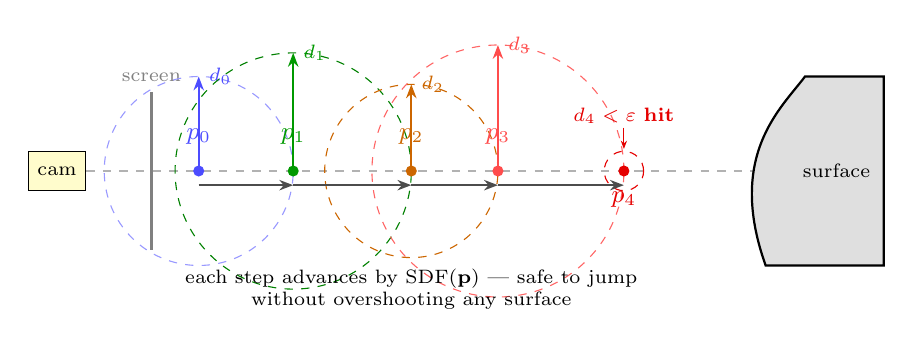
\begin{tikzpicture}[
  arr/.style={-{Stealth[length=5pt]}, thick},
  lbl/.style={font=\small},
]

%% Camera
\node[draw, fill=yellow!20, minimum width=0.7cm, minimum height=0.5cm,
      font=\scriptsize] (cam) at (0, 0) {cam};

%% Screen plane
\draw[thick, gray] (1.2, -1.0) -- (1.2, 1.0)
  node[above, font=\scriptsize, gray] {screen};

%% Ray direction
\draw[arr, dashed, gray!60] (cam.east) -- (10.5, 0);

%% Surface (implicit blob)
\draw[thick, fill=gray!25]
  (9.0, -1.2) .. controls (8.5,0.2) and (9.2,0.8) .. (9.5, 1.2)
  -- (10.5, 1.2) -- (10.5,-1.2) -- cycle;
\node[font=\scriptsize] at (9.9, 0) {surface};

%% March steps and SDF spheres
% step 0: origin of march (after screen)
\coordinate (p0) at (1.8, 0);
\def\ra{1.2}
\draw[blue!40, dashed] (p0) circle (\ra);
\fill[blue!70] (p0) circle (2pt);
\node[lbl, above=6pt, blue!70] at (p0) {$p_0$};
\draw[arr, blue!70] (p0) -- ++(0, \ra) node[right, font=\scriptsize]{$d_0$};

% step 1
\coordinate (p1) at (3.0, 0);
\def\rb{1.5}
\draw[green!50!black, dashed] (p1) circle (\rb);
\fill[green!60!black] (p1) circle (2pt);
\node[lbl, above=6pt, green!60!black] at (p1) {$p_1$};
\draw[arr, green!60!black] (p1) -- ++(0, \rb) node[right, font=\scriptsize]{$d_1$};

% step 2
\coordinate (p2) at (4.5, 0);
\def\rc{1.1}
\draw[orange!80!black, dashed] (p2) circle (\rc);
\fill[orange!80!black] (p2) circle (2pt);
\node[lbl, above=6pt, orange!80!black] at (p2) {$p_2$};
\draw[arr, orange!80!black] (p2) -- ++(0, \rc) node[right, font=\scriptsize]{$d_2$};

% step 3
\coordinate (p3) at (5.6, 0);
\def\rd{1.6}
\draw[red!60, dashed] (p3) circle (\rd);
\fill[red!70] (p3) circle (2pt);
\node[lbl, above=6pt, red!70] at (p3) {$p_3$};
\draw[arr, red!70] (p3) -- ++(0, \rd) node[right, font=\scriptsize]{$d_3$};

% step 4 (hit)
\coordinate (p4) at (7.2, 0);
\def\re{0.25}
\draw[red!90!black, dashed] (p4) circle (\re);
\fill[red!90!black] (p4) circle (2pt);
\node[lbl, below=4pt, red!90!black] at (p4) {$p_4$};
\node[font=\scriptsize, red!90!black] at (7.2, 0.7) {$d_4 < \varepsilon$\ \textbf{hit}};
\draw[-{Stealth[length=3pt]}, red!90!black] (7.2, 0.55) -- (7.2, 0.28);

%% step arrows along ray
\foreach \x/\nx in {1.8/3.0, 3.0/4.5, 4.5/5.6, 5.6/7.2} {
  \draw[arr, thick, black!70] (\x, -0.18) -- (\nx, -0.18);
}

%% annotation
\node[font=\scriptsize, align=center] at (4.5, -1.5)
  {each step advances by $\mathrm{SDF}(\mathbf{p})$ --- safe to jump\\
   without overshooting any surface};

\end{tikzpicture}
\label{fig:raymarching}
\end{figure}
Ray marching: the ray advances by the SDF value at each step.
The SDF gives the radius of an empty sphere centred at $\mathbf{p}$,
so stepping that distance is guaranteed not to cross any surface.
Iteration stops when $\mathrm{SDF}(\mathbf{p}) < \varepsilon$ (hit) or
the step count exceeds \texttt{MAX\_ITER} (miss).

\section{Difficulties in Ray Marching on a CPU, and the GPU Baseline}

Ray marching is one of the most natural algorithms for a massively parallel
processor and one of the worst for a general-purpose CPU. Understanding why
illuminates the design decisions made throughout this project.

\subsection{Why the CPU Struggles}

A CPU core is optimised for sequential execution with data-dependent
instructions. Ray marching violates this by being embarrassingly parallel per
pixel, but the CPU cannot exploit that independence without SIMD vectorisation,
and the march loop introduces \textbf{divergence}: each pixel exits after a
different number of iterations, so SIMD lanes stall waiting for the worst case.
Beyond divergence, the SDF evaluation is a long floating-point dependency chain
that stalls an in-order processor like the ARM Cortex-A9 at every step. The
result is approximately 0.3--1\,fps at $1024\times600$ which is far from real-time.

\subsection{The GPU Baseline: GLSL Fragment Shaders}

GPUs tolerate divergence by running warps of 32 threads in lockstep and masking
divergent lanes rather than retiring them, hiding the cost behind thousands of
other warps in flight. GLSL fragment shaders express this naturally: the GPU
calls \texttt{main()} once per pixel, and the entire march loop, SDF evaluation,
and colour mapping form a single \texttt{.frag} file. The software prototyping
environment comprises thirteen such files, each implementing a complete scene in
WebGL2 and runnable in any browser.

The scaffold shader's \texttt{mod()} for space repetition maps directly onto
\texttt{fp\_modulus} in SystemVerilog; the \texttt{for} loop with
\texttt{break} on hit maps onto the feedback-loop architecture; and
\texttt{MAX\_ITER\,=\,128} is identical in both. An RTX 3090 runs comparable
scenes at 60\,fps even at $2560\times1440$, winning by issuing thousands of
parallel FP32 operations per cycle across dedicated shader cores.

\subsection{What the FPGA Does Differently}

The FPGA does not compete with the GPU on raw throughput, it simply cannot! What
we demonstrate through this implemenation is that the \textit{same algorithm} can be implemented in
custom fixed-function hardware on a \£125 embedded board without a GPU, at
real-time frame rates, using a custom floating-point format designed around
the specific arithmetic units available on the device.

The key architectural insight is that ray marching's embarrassing parallelism
does not require thousands of cores - it requires a deep pipeline that can
keep all stages occupied simultaneously. With a 163-cycle pipeline latency
and 1 pixel/cycle throughput per core, two \texttt{march\_core} instances
retire 2 pixels every clock cycle. At 125\,MHz this is
$2.5\times10^8$\,pixels/s before accounting for multi-iteration feedback -
placing the FPGA's throughput within an order of magnitude of an optimised
single-threaded x86 software renderer (AVX2 ISA, for example), while running on a \£125 embedded SoC
at a fraction of the power.

The GLSL prototyping methodology was essential: each scene was validated
visually in the browser before a single line of SystemVerilog was written.
Because the GLSL and RTL share the same mathematical structure - the same
SDFs, the same march loop, the same hit threshold-- bugs in the RTL
produced visually wrong output that could be diagnosed by comparison against
the reference shader. The \texttt{.frag} files are not separate work; they
are the algorithmic specification that the hardware implements! Essentially, our work consisted in replicating the GSLS exactly, as seen by the comments left on code referencing pieces of GLSL.

\section{Project Structure and Methodology}

\paragraph{Prototyping approach -}
Development followed a prototype-then-synthesise methodology, as well as quick sprint/Waterfall agile approach. Each SDF scene
was first written as a GLSL fragment shader running in a browser (WebGL2),
allowing rapid visual iteration on scene geometry, camera behaviour, and
colour mapping without a Vivado compile cycle. Once a scene was validated in
GLSL, it was translated to SystemVerilog using the 27-bit FP library and
integrated into the march pipeline. This separation of algorithmic
correctness (GLSL) from timing correctness (RTL) significantly reduced the
number of full synthesis runs needed.

\paragraph{Design decisions along the way -}
Several significant design pivots were made during the project in response to
practical constraints discovered during implementation:

\begin{itemize}
\item \textbf{BRAM framebuffer $\rightarrow$ DDR VDMA.} The initial HDMI design used an on-chip BRAM framebuffer with a custom scan-out
controller. At $1024\times600\times32$\,bit, the framebuffer requires
24.6\,Mbit - far exceeding the 4.9\,Mbit of available BRAM. The design was
replaced with an AXI VDMA IP reading from DDR3, freeing all on-chip BRAM for
pipeline registers and avoiding the throughput bottleneck of BRAM arbitration
between the writer and scan-out.

\item \textbf{Hardware FFT IP $\rightarrow$ Software FFT.} The  initial
design used Xilinx FFT IP with AXI-DMA to compute frequency bands in hardware.
This consumed significant PL resources (over 3000 LUTs), that prevented multicore from fitting on the board. The design was simplified: FFT computation moved
entirely to the host PC using NumPy, and only the 11 resulting feature floats
are streamed to the PYNQ over TCP. This was decided after observation that the PYNQ board does not have audio line in through jack. This reduced PL resource usage and
eliminated a source of integration complexity at the cost of requiring a
connected PC during music-reactive mode.

\item \textbf{Fixed-point $\rightarrow$ 27-bit floating-point.} Early RTL used
Q2.29 fixed-point arithmetic. Ray marching requires evaluating distances that
span several orders of magnitude; from sub-millimetre hit thresholds to
several-unit step sizes! This caused precision loss and visual artefacts in
fixed-point. Moreover, given we could only represent [-2;2] values, our scenes were very limited. A custom 27-bit floating-point format was adopted, giving the same
exponent range as IEEE\,754 single precision (8-bit exponent) with a reduced
18-bit mantissa. This trades $\sim$5\,bits of mantissa precision for a 5-bit
reduction in word width, saving DSP and routing resources while retaining
sufficient dynamic range for the march algorithm. Indeed, the PYNQ Z1 DSPs are 25 x 18 - using full IEEE\,754 precision would have doubled DSP count, splitting computations in two.

\item \textbf{Single-core $\rightarrow$ dual-core.} The initial design had a
single \texttt{march\_core}. Profiling showed the SDF evaluation pipeline
(107-clock latency) was the throughput bottleneck; adding a second core fed by
a round-robin dispatcher doubled pixel throughput with minimal latency cost, as the feedback controller and framebuffer writer could be
shared. However, this demanded deep hardware Verilog -> Logic Gates inference thinking, moving the feedback fifo to BRAM and other tradeoffs. Indeed, each core is about 17,500 LUTs!
\end{itemize}

\paragraph{Testing methodology:}
Module-level simulation was used throughout. Each FP primitive, the ray
generator, pixel dispatcher, feedback controller, and framebuffer writer have
standalone testbenches run via Verilator simulations with GoogleTest assertions verifications in temporary scripts. The full-system
integration testbench confirmed zero-duplicate pixel emission across all
921\,600 pixels. RTL modules were cross-tested by members other than the
original author. Final validation was on the physical PYNQ-Z1 board, with
visual inspection of the rendered output against the GLSL reference.

% --- RECOMPRESSED FORCE TO BOTTOM CONTAINER ---
\vspace{\fill} 
\begin{center}
    \nopagebreak % Strictly prevents a page break right before the image block
    \begin{minipage}{0.5\textwidth} % Slightly downscaled width from 0.85 to open up vertical budget
        \centering
        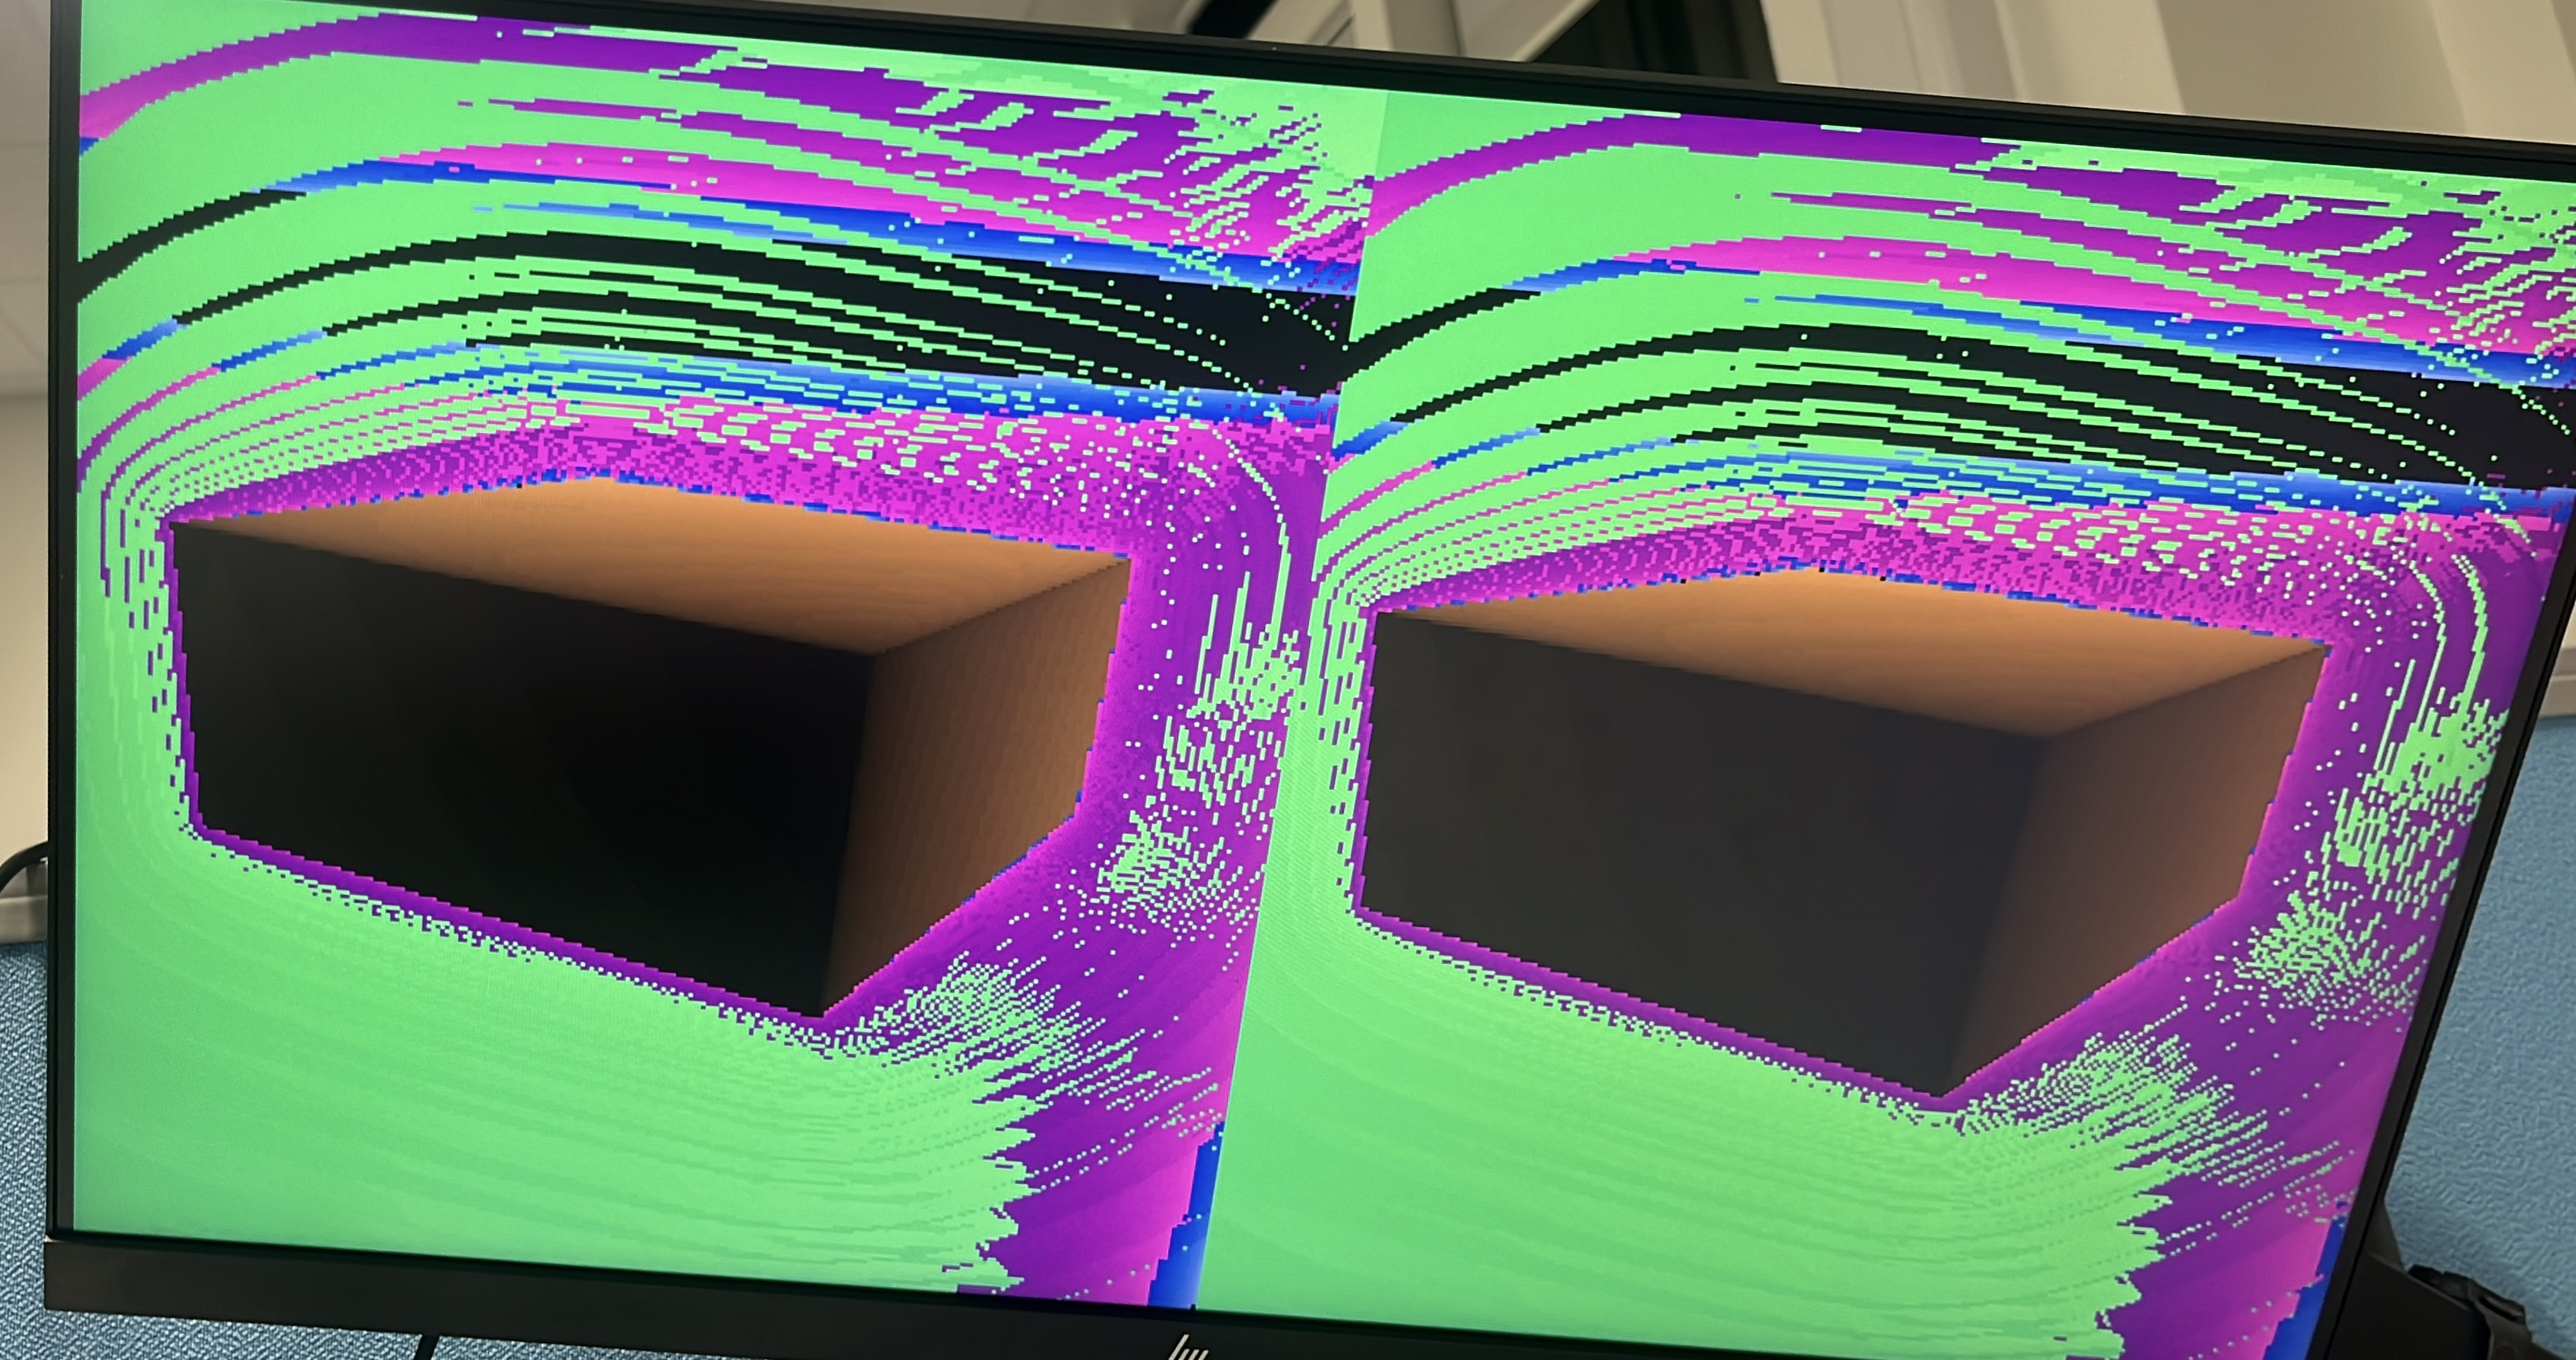
\includegraphics[width=\textwidth]{imgs/box_no_infinite.JPG}
        \vspace{-0.1cm} % Tighter padding between image and text
        \captionof{figure}{Initial renders of the box SDF, without space repetition. Notice the repeating colors in world borders due to palette.sv cyclical nature. 33 frames per second.}
        \label{fig:your_label}
    \end{minipage}
\end{center}

% Chapter 2 — System Components and Design
% Chapter 2 — System Components and Design
% Input this file from the main document, which must have in its preamble:
%   \usepackage{listings}  \usepackage{xcolor}  \usepackage{amsmath}
%   \usepackage{amssymb}   \usepackage{booktabs} \usepackage{array}
%   \usepackage{placeins}  \usepackage{enumitem} \usepackage{caption}
%   \usepackage{needspace} \usepackage{etoolbox} \usepackage{setspace}
%   \usepackage{tikz}
%   \usetikzlibrary{positioning, arrows.meta, fit, backgrounds}
%
% Also define in preamble (or here once):
%   \definecolor{codebg}{HTML}{F5F5F5}
%   \definecolor{codeframe}{HTML}{CCCCCC}
%   \definecolor{codecomment}{HTML}{6A737D}
%   \definecolor{codestring}{HTML}{032F62}
%   \definecolor{codekeyword}{HTML}{D73A49}
%   \lstdefinestyle{clean}{...}  (see below)
%   \newcommand{\code}[1]{\texttt{#1}}

\definecolor{codebg}{HTML}{F5F5F5}
\definecolor{codeframe}{HTML}{CCCCCC}
\definecolor{codecomment}{HTML}{6A737D}
\definecolor{codestring}{HTML}{032F62}
\definecolor{codekeyword}{HTML}{D73A49}

\lstdefinestyle{clean}{
    backgroundcolor=\color{codebg},
    basicstyle=\ttfamily\small\linespread{1.1}\selectfont,
    breaklines=true,
    breakatwhitespace=true,
    frame=single,
    framerule=0.4pt,
    rulecolor=\color{codeframe},
    xleftmargin=0.75em,
    xrightmargin=0.75em,
    aboveskip=0.8em,
    belowskip=0.8em,
    showstringspaces=false,
    tabsize=4,
    commentstyle=\color{codecomment}\itshape,
    keywordstyle=\color{codekeyword}\bfseries,
    stringstyle=\color{codestring},
    extendedchars=true,
    keepspaces=true,
    captionpos=b,
    numbers=none,
}
\lstset{style=clean}

\providecommand{\code}[1]{\texttt{#1}}
\usetikzlibrary{positioning, arrows.meta, fit, backgrounds}

\makeatletter
\titleformat{\chapter}[block]
  {\normalfont\huge\bfseries\color{ImperialBlue}}
  {\thechapter}{20pt}{\huge}
\titlespacing*{\chapter}{0pt}{-20pt}{15pt}
\makeatother

\titlespacing*{\paragraph}{0pt}{0.4ex}{0.2ex}

\chapter{System Components and Design}
\label{ch2}

\begin{spacing}{0.3}
\minitoc
\end{spacing}

\thesisspacing


% ===============================================================
\section{System Overview}
% ===============================================================

This chapter gives a detailed breakdown of each hardware and software subsystem,
with a mathematically rigorous treatment of ray marching and the custom
arithmetic that makes it feasible in hardware. Figure~\ref{fig:system_arch}
shows the full system architecture.

The rendering pipeline is a deeply pipelined hardware datapath on the
programmable logic (PL). Pixel coordinates enter \code{pixel\_dispatch}, flow
through ray generation (48 cycles), enter the SDF evaluation stage inside
\code{march\_core} (107 cycles), advance along the ray in the step unit (8
cycles), and either terminate (hit or max iterations) or re-enter the pipeline
via \code{feedback\_ctrl} for another sphere-tracing iteration. Completed pixels
are burst to DDR3 by the AXI framebuffer writer, and the VDMA IP streams the
completed frame to the HDMI display at $1024\times600$ pixels.

Two independent input streams modulate the scene in real time. \textbf{Camera
orientation} is supplied by an MPU-6050 inertial measurement unit connected to
the PS over I$^2$C. Raw accelerometer and gyroscope readings are fused in a
complementary filter running on the ARM Cortex-A9 (\code{ctrl.py}) to produce
pitch, roll, and yaw estimates. These are used to construct a $3\times3$ lookat
matrix, which is written each frame to the AXI-Lite camera register file at
\texttt{0x43C00000} alongside the camera origin. \textbf{Music reactivity} is
supplied by a 1024-point FFT pipeline running on the host PC. Per audio block,
bass, mid, and treble energy bands, RMS, spectral centroid, zero-crossing rate,
and a beat detection flag are computed and streamed over TCP. The PS receives
these eleven features and writes them directly into the AXI-Lite SDF parameter
registers, where the PL picks them up at the start of each SDF evaluation.

\begin{figure}[htbp]
\centering
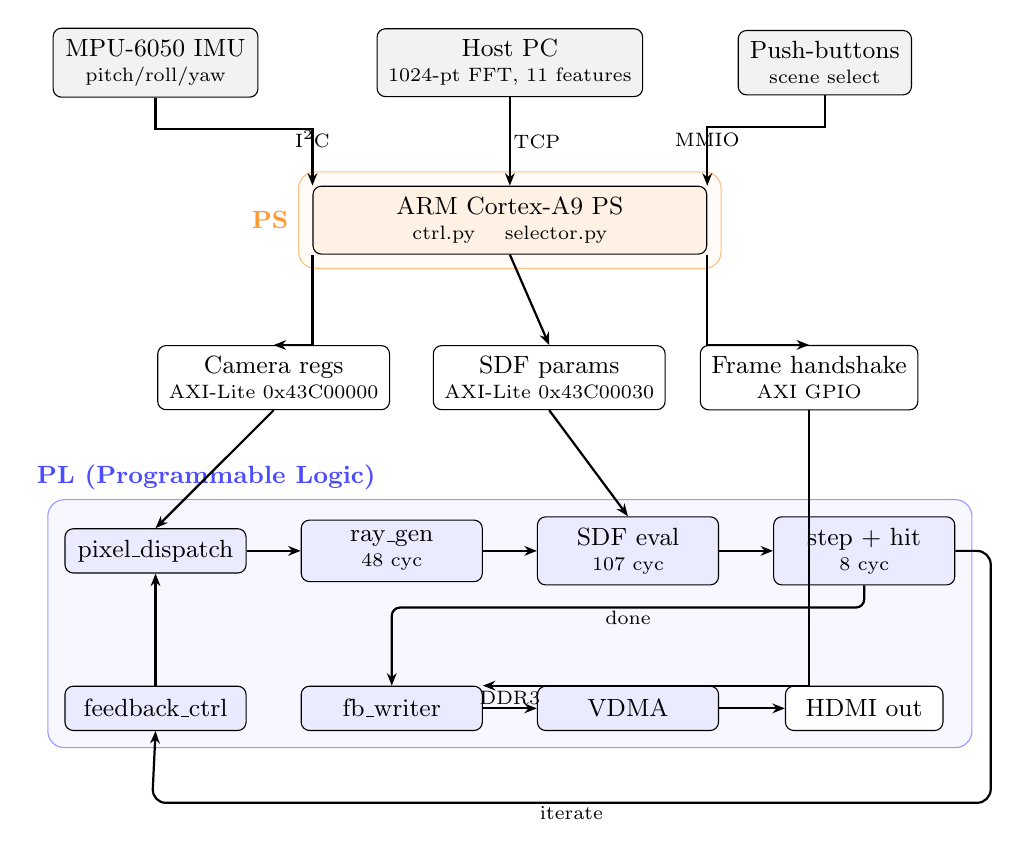
\begin{tikzpicture}[
    box/.style   ={draw, rounded corners=3pt, align=center,
                   minimum height=1.6em, inner sep=4pt, font=\small, fill=white},
    extbox/.style={box, fill=gray!10},
    psbox/.style ={box, fill=orange!10},
    plbox/.style ={box, fill=blue!8},
    arr/.style   ={-{Stealth[length=4.5pt, width=3.5pt]}, thick},
    lbl/.style   ={font=\scriptsize, inner sep=1pt}
]

%% ── External sources (top row) ───────────────────────────────────
\node[extbox, minimum width=2.6cm] (imu)    at (0,    0)
    {MPU-6050 IMU\\[-2pt]{\scriptsize pitch/roll/yaw}};
\node[extbox, minimum width=2.6cm] (hostpc) at (4.5,  0)
    {Host PC\\[-2pt]{\scriptsize 1024-pt FFT, 11 features}};
\node[extbox, minimum width=2.2cm] (btns)   at (8.5,  0)
    {Push-buttons\\[-2pt]{\scriptsize scene select}};

%% ── PS ───────────────────────────────────────────────────────────
\node[psbox, minimum width=5.0cm] (ps) at (4.5, -2.0)
    {ARM Cortex-A9 PS\\[-2pt]{\scriptsize ctrl.py \quad selector.py}};

%% ── AXI register interfaces ──────────────────────────────────────
\node[box, minimum width=2.8cm] (camregs) at (1.5, -4.0)
    {Camera regs\\[-2pt]{\scriptsize AXI-Lite 0x43C00000}};
\node[box, minimum width=2.8cm] (sdfp)    at (5.0, -4.0)
    {SDF params\\[-2pt]{\scriptsize AXI-Lite 0x43C00030}};
\node[box, minimum width=2.6cm] (gpiohsk) at (8.3, -4.0)
    {Frame handshake\\[-2pt]{\scriptsize AXI GPIO}};

%% ── PL pipeline row 1 ────────────────────────────────────────────
\node[plbox, minimum width=2.3cm] (dispatch) at (0,   -6.2)
    {pixel\_dispatch};
\node[plbox, minimum width=2.3cm] (rg)       at (3.0, -6.2)
    {ray\_gen\\[-2pt]{\scriptsize 48 cyc}};
\node[plbox, minimum width=2.3cm] (sdfev)    at (6.0, -6.2)
    {SDF eval\\[-2pt]{\scriptsize 107 cyc}};
\node[plbox, minimum width=2.3cm] (steph)    at (9.0, -6.2)
    {step + hit\\[-2pt]{\scriptsize 8 cyc}};

%% ── PL pipeline row 2 (feedback + output) ────────────────────────
\node[plbox, minimum width=2.3cm] (fbctrl)  at (0,   -8.2)
    {feedback\_ctrl};
\node[plbox, minimum width=2.3cm] (fbwrite) at (3.0, -8.2)
    {fb\_writer};
\node[plbox, minimum width=2.3cm] (vdma)    at (6.0, -8.2)
    {VDMA};
\node[box,   minimum width=2.0cm] (hdmi)    at (9.0, -8.2)
    {HDMI out};

%% ── External → PS ────────────────────────────────────────────────
\draw[arr] (imu.south)  -- ++(0,-0.4) -| node[lbl, above, pos=0.7]{I$^2$C} (ps.north west);
\draw[arr] (hostpc)     -- node[lbl, right]{TCP} (ps.north);
\draw[arr] (btns.south) -- ++(0,-0.4) -| node[lbl, above, pos=0.7]{MMIO}   (ps.north east);

%% ── PS → AXI interfaces ──────────────────────────────────────────
\draw[arr] (ps.south west) |- (camregs.north);
\draw[arr] (ps.south)      -- (sdfp.north);
\draw[arr] (ps.south east) |- (gpiohsk.north);

%% ── AXI → PL ─────────────────────────────────────────────────────
\draw[arr] (camregs.south) -- (dispatch.north);
\draw[arr] (sdfp.south)    -- (sdfev.north);
\draw[arr] (gpiohsk.south) |- (fbwrite.north east);

%% ── Pipeline datapath ────────────────────────────────────────────
\draw[arr] (dispatch) -- (rg);
\draw[arr] (rg)       -- (sdfev);
\draw[arr] (sdfev)    -- (steph);

%% ── Done pixels: steph → fbwrite (route through gap between rows)
\draw[arr, rounded corners=3pt]
    (steph.south) -- ++(0,-0.28)
    -- node[lbl, below]{done} ++(-6.0,0)
    -- (fbwrite.north);

%% ── Iterate: steph → loop around right → fbctrl.south ──────────
\draw[arr, rounded corners=5pt]
    (steph.east) -- ++(0.45,0) -- ++(0,-3.2)
    -- node[lbl, below]{iterate} ++(-10.65,0)
    -- (fbctrl.south);

%% ── fbctrl feeds back to dispatch ───────────────────────────────
\draw[arr] (fbctrl.north) -- (dispatch.south);

%% ── Output path ──────────────────────────────────────────────────
\draw[arr] (fbwrite) -- node[lbl, above]{DDR3} (vdma);
\draw[arr] (vdma)    -- (hdmi);

%% ── Background shading ───────────────────────────────────────────
\begin{scope}[on background layer]
    \node[draw=blue!40, fill=blue!3, rounded corners=6pt,
          inner sep=6pt,
          fit=(dispatch)(rg)(sdfev)(steph)(fbctrl)(fbwrite)(vdma)(hdmi),
          label={[font=\small\bfseries, text=blue!70]above left:PL (Programmable Logic)}
    ] {};
    \node[draw=orange!50, fill=orange!3, rounded corners=6pt,
          inner sep=5pt,
          fit=(ps),
          label={[font=\small\bfseries, text=orange!80]left:PS}
    ] {};
\end{scope}

\end{tikzpicture}
\caption{Full system architecture, more on this in Section 3, Integration. IMU and host-PC FFT
feed the ARM PS, which programs the PL over AXI-Lite each frame. The PL pipeline traces rays in a
feedback loop and streams completed frames to HDMI via VDMA.}
\label{fig:system_arch}
\end{figure}

\FloatBarrier


% ===============================================================
\section{Custom 27-bit Floating-Point Format}
\label{sec:fp}
% ===============================================================

\subsection{Format and Motivation}

The entire hardware rendering pipeline uses a custom 27-bit floating-point
format rather than IEEE\,754 single precision (32-bit) or fixed-point arithmetic.
The format is \texttt{\{sign[26], exponent[25:18], mantissa[17:0]\}}: one sign
bit, an eight-bit biased exponent identical to IEEE\,754 (bias 127), and an
eighteen-bit mantissa with an implicit leading 1. This gives the same dynamic
range as IEEE\,754 single precision with exponents from $2^{-126}$ to $2^{127}$ 
while reducing the word width by five bits.

\begin{table}[htbp]
\centering
\small
\caption{Floating-point formats across the project}
\label{tab:fp_formats}
{\renewcommand{\arraystretch}{1.4}
\begin{tabular}{lcccc}
\toprule
\textbf{Format} & \textbf{Sign} & \textbf{Exponent} & \textbf{Mantissa} & \textbf{Total} \\
\midrule
IEEE-754 float32       & 1 & 8     & 23      & 32 bits \\
Project FP27           & 1 & 8     & 18      & 27 bits \\
Q4.12 (neural weights) & 1 & 4 int & 12 frac & 16 bits \\
\bottomrule
\end{tabular}}
\end{table}

\FloatBarrier

\subsection{Bit Layout and Worked Conversions}

Figure~\ref{fig:fp27_bits} shows the 27-bit field breakdown. The exponent is
biased at 127 (= \texttt{0b01111111}) so that the zero exponent is represented
as \texttt{0b10000000}, matching IEEE\,754 and allowing the same exponent
arithmetic ie negative exponents as well as positive exponents. The mantissa carries an implicit leading 1 bit, so the full
represented mantissa is $1.m_{17}m_{16}\cdots m_0$.

\begin{figure}[htbp]
\centering
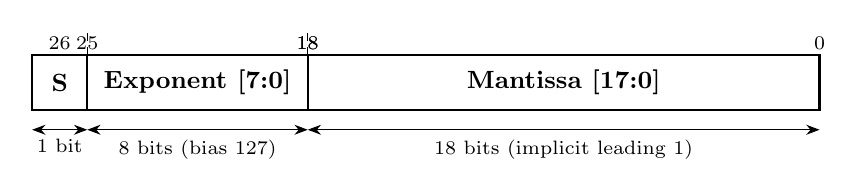
\begin{tikzpicture}[font=\small]
    % Bit-field rectangles
    \draw[thick] (0,0) rectangle (0.7, 0.7);   % bit 26: sign
    \draw[thick] (0.7,0) rectangle (3.5, 0.7); % bits 25:18 exponent (8 bits)
    \draw[thick] (3.5,0) rectangle (10.0, 0.7);% bits 17:0 mantissa (18 bits)

    % Labels inside boxes
    \node at (0.35, 0.35) {\textbf{S}};
    \node at (2.1,  0.35) {\textbf{Exponent [7:0]}};
    \node at (6.75, 0.35) {\textbf{Mantissa [17:0]}};

    % Bit indices above
    \node[font=\scriptsize] at (0.35, 0.85) {26};
    \node[font=\scriptsize] at (0.7,  0.85) {25};
    \node[font=\scriptsize] at (3.5,  0.85) {18};
    \node[font=\scriptsize] at (3.5,  0.85) {18};
    \node[font=\scriptsize] at (10.0, 0.85) {0};
    \draw[densely dashed] (0.7, 0.7) -- (0.7, 1.0);
    \draw[densely dashed] (3.5, 0.7) -- (3.5, 1.0);

    % Width annotations below
    \draw[<->, >=Stealth] (0, -0.25) -- node[below, font=\scriptsize]{1 bit} (0.7, -0.25);
    \draw[<->, >=Stealth] (0.7, -0.25) -- node[below, font=\scriptsize]{8 bits (bias 127)} (3.5, -0.25);
    \draw[<->, >=Stealth] (3.5, -0.25) -- node[below, font=\scriptsize]{18 bits (implicit leading 1)} (10.0, -0.25);
\end{tikzpicture}
\caption{FP27 bit field layout: 1 sign, 8 exponent (bias 127), 18 mantissa.}
\label{fig:fp27_bits}
\end{figure}

\FloatBarrier

\paragraph{Converting a decimal value to FP27.}\newline
As a concrete example, convert $-3.5$ to FP27.
\begin{enumerate}[noitemsep]
    \item \textbf{Sign:} negative $\implies s = 1$.
    \item \textbf{Exponent:} $3.5 = 1.75 \times 2^1$, so the unbiased exponent
          is $1$, and the stored exponent is $e = 127 + 1 = 128 =
          \texttt{0b10000000}$.
    \item \textbf{Mantissa:} the fractional part is $0.75$. In binary:
          $0.75 = 0.11_2$, giving mantissa bits $m = \texttt{11\,0000\,0000\,0000\,0000}$
          ($0.75 \times 2^{18} = 196608 = \texttt{0x30000}$).
    \item \textbf{Result:}
          \[
              \texttt{1\_10000000\_110000000000000000} = \texttt{27'hC30000}
          \]
\end{enumerate}

\paragraph{Converting FP27 back to decimal.}\newline
Given \texttt{27'h1E40000}: $s{=}0$, $e{=}\texttt{0x3C}{=}60$, $m{=}\texttt{0x40000}{=}262144$.
\[
    \text{value} = (-1)^0 \times (1 + 262144/2^{18}) \times 2^{60-127}
    = 1.5 \times 2^{-67} \approx 1.02 \times 10^{-20}
\]
This illustrates the extreme dynamic range the format provides: representing
$\sim 10^{-20}$ exactly is impossible in Q2.29 fixed point but trivial in FP27.

\paragraph{Conversion from IEEE\,754 in software.}\newline
The Python controller uses the following to pack FP27 values into AXI registers
(truncating the bottom 5 mantissa bits):
\begin{lstlisting}[language=Python]
def fp32_to_fp27(value):
    bits      = struct.unpack(">I", struct.pack(">f", float(value)))[0]
    sign      = (bits >> 31) & 0x1
    exponent  = (bits >> 23) & 0xFF      # same 8-bit biased exponent
    frac23    = bits & 0x7FFFFF
    frac18    = (frac23 + 0x10) >> 5     # round, then drop bottom 5 bits
    return (sign << 26) | (exponent << 18) | frac18
\end{lstlisting}
The exponent is identical between IEEE\,754 and FP27 (same bias, same width), so
no conversion is needed there --- only the mantissa is truncated.

\paragraph{Why not fixed-point? }\mbox{}\newline
Ray marching requires evaluating distances that span several orders of magnitude
in a single frame. The hit threshold is approximately $10^{-3}$ (a ray is
considered to have struck a surface when the SDF returns a value smaller than
this); the maximum step size can reach several scene units. A fixed-point format
must accommodate both extremes simultaneously. The Q2.29 format used in early
RTL could only represent values in $[-2, 2]$, which immediately constrained
scene scale and caused precision collapse as distances accumulated over 128
iterations. Floating-point represents each value relative to its own magnitude,
so small distances near surfaces remain precise regardless of how far the ray
has travelled.

\paragraph{Why 27 bits, not 32?}\mbox{}\newline
The Xilinx PYNQ-Z1 contains DSP48E1 slices whose multiplier operates on
$18 \times 25$ bit inputs. IEEE\,754 single precision requires a $24 \times 24$
bit mantissa multiply (including the implicit leading bit), which exceeds the
18-bit input port and forces Vivado to cascade two DSP blocks per multiply. With
an 18-bit mantissa, the product $(1.\text{mantissa}) \times (1.\text{mantissa})$
fits in one DSP48E1 exactly: the 19-bit inputs ($1 +$ 18 mantissa bits) produce
a 38-bit product, which is truncated to 18 bits after normalisation. Using
27-bit FP therefore halves the DSP count per multiply relative to IEEE\,754,
directly determining whether the design fits on chip. The five mantissa bits
sacrificed cause a maximum relative error of $2^{-18} \approx 3.8 \times
10^{-6}$, which is invisible at $1024 \times 600$ or $512 \times 300$ pixel
resolution. The mantissa carries an implicit leading 1, which comes at the cost
of not being able to represent subnormal numbers. Given our purpose (real-time
psychedelic renders, not pixel-perfect scientific computation) this was an
explicit decision not to pursue subnormals. This follows traditional baseline
GPU architecture: subnormal handling typically requires a kernel trap to the CPU
which is an extensive overhead and is omitted in most GPU shader cores for the same
reason.


% ===============================================================
\section{Floating-Point Library}
\label{sec:fplibrary}
% ===============================================================

\subsection{Library Overview}

The FP library comprises 16 fully pipelined synthesisable Verilog modules,
each accepting a new input every clock cycle and producing a result after a
fixed latency with no stall or handshake signals. Pipeline synchronisation
between modules of differing latencies is handled exclusively by
\code{state\_pipe} delay lines. SRT division and Goldschmidt's algorithm were
evaluated before settling on Newton-Raphson reciprocal for its fixed-latency
amenability.

\begin{table}[htbp]
\centering
\small
\caption{27-bit FP library modules and pipeline latencies}
\label{tab:fp_lib}
{\renewcommand{\arraystretch}{1.3}
\begin{tabular}{llc}
\toprule
\textbf{Module} & \textbf{Operation} & \textbf{Latency (cycles)} \\
\midrule
\code{fp\_mul.v}            & Multiply                            & 4  \\
\code{fp\_add.v}            & Add                                 & 4  \\
\code{fp\_sub.v}            & Subtract                            & 4  \\
\code{fp\_inverse.sv}       & $1/b$ via Newton-Raphson            & 36 \\
\code{fp\_division.sv}      & $a/b = a \times (1/b)$              & 40 \\
\code{fp\_isqrt.v}          & $1/\sqrt{x}$ via NR + magic number  & 16 \\
\code{fp\_length.v}         & $\|\mathbf{v}\|$                    & 32 \\
\code{fp\_modulus.sv}       & $a \bmod b$ for space repetition    & 52 \\
\code{fp\_floor.sv}         & $\lfloor a \rfloor$ (combinational) & 0  \\
\code{fp\_abs.v}            & $|a|$ (combinational)               & 0  \\
\code{fp\_negate.v}         & $-a$ (combinational)                & 0  \\
\code{fp\_min.v}            & $\min(a,b)$ (combinational)         & 0  \\
\code{fp\_max.v}            & $\max(a,b)$ (combinational)         & 0  \\
\code{int2fp.v}             & Integer $\to$ FP27                  & 1  \\
\code{fp\_normalize.sv}     & Normalise FP27 vector               & 8  \\
\code{fp\_mul\_vec3\_mat33.sv} & $3\times3$ matrix $\times$ vector & 8  \\
\bottomrule
\end{tabular}}
\end{table}

\FloatBarrier

\subsection{Multiplication - \code{fp\_mul.v}}

Two FP27 numbers $a$ and $b$ are multiplied as:
\[
    \text{sign} = a_s \oplus b_s, \quad
    \text{exp} = e_a + e_b - 127, \quad
    \text{mant} = (1.m_a) \times (1.m_b)
\]
The $19\times19$-bit mantissa product yields 38 bits; overflow (product $\geq
2$) shifts the mantissa right and increments the exponent. The four-stage
pipeline is: (1) register inputs; (2) DSP48E1 multiply with
\lstinline[language=Verilog]{(* use_dsp = "yes" *)}; (3) register raw DSP
output, breaking the carry chain from normalisation; (4) normalise and
propagate zero flag. Stage 3 is critical: without it, the normalisation mux
sits combinationally on the DSP output, creating a 12\,ns path and failing
timing at 125\,MHz. The extra register reduces the worst-case path to under
7\,ns.

\subsection{Addition - \code{fp\_add.v}}

The four-stage pipeline aligns operands to the same exponent, adds or subtracts
mantissas, then renormalises. The \code{(* keep = "true" *)} pragma prevents
Vivado from merging intermediate comparison wires into a single wide comparator
that would exceed the timing budget.

\subsection{Inverse Square Root - \code{fp\_isqrt.v}}
\label{sec:isqrt}

The inverse square root $y = x^{-1/2}$, required by \code{fp\_length} and
\code{fp\_normalize}, is implemented via the Quake~III fast inverse square root
technique with one Newton-Raphson refinement. Defining $f(y) = y^{-2} - x$,
the Newton-Raphson update is:
\[
    y_{n+1} = y_n\!\left(\tfrac{3}{2} - \tfrac{x}{2}\,y_n^2\right)
\]
The initial estimate exploits the integer reinterpretation $I(x^{-1/2}) \approx
\frac{3}{2}B\cdot2^P - I(x)/2$, implemented as a single combinational
subtraction:
\begin{lstlisting}[language=Verilog]
assign y0 = magic_number - (a >> 1);
\end{lstlisting}
where $0.5x$ is computed by decrementing the exponent field by one, avoiding
an extra multiply. The Newton-Raphson chain is four \code{fp\_mul}/\code{fp\_sub}
stages of 4 cycles each; total latency: 16 cycles.

\paragraph{Magic constant for FP27.}
From $\log_2 x \approx I(x)/2^P - B$, solving for $I(y)$ with $y = x^{-1/2}$
gives $M = \frac{3}{2}\times127\times2^P$. For $P=18$: $M_{27} =
49{,}938{,}432 = \texttt{0x2F9B400}$, empirically refined to
\texttt{27'h2F9B8CF}.

\begin{center}
    \nopagebreak % Prevents LaTeX from sticking a pagebreak mid-container
    \begin{minipage}{0.48\textwidth}
        \centering
        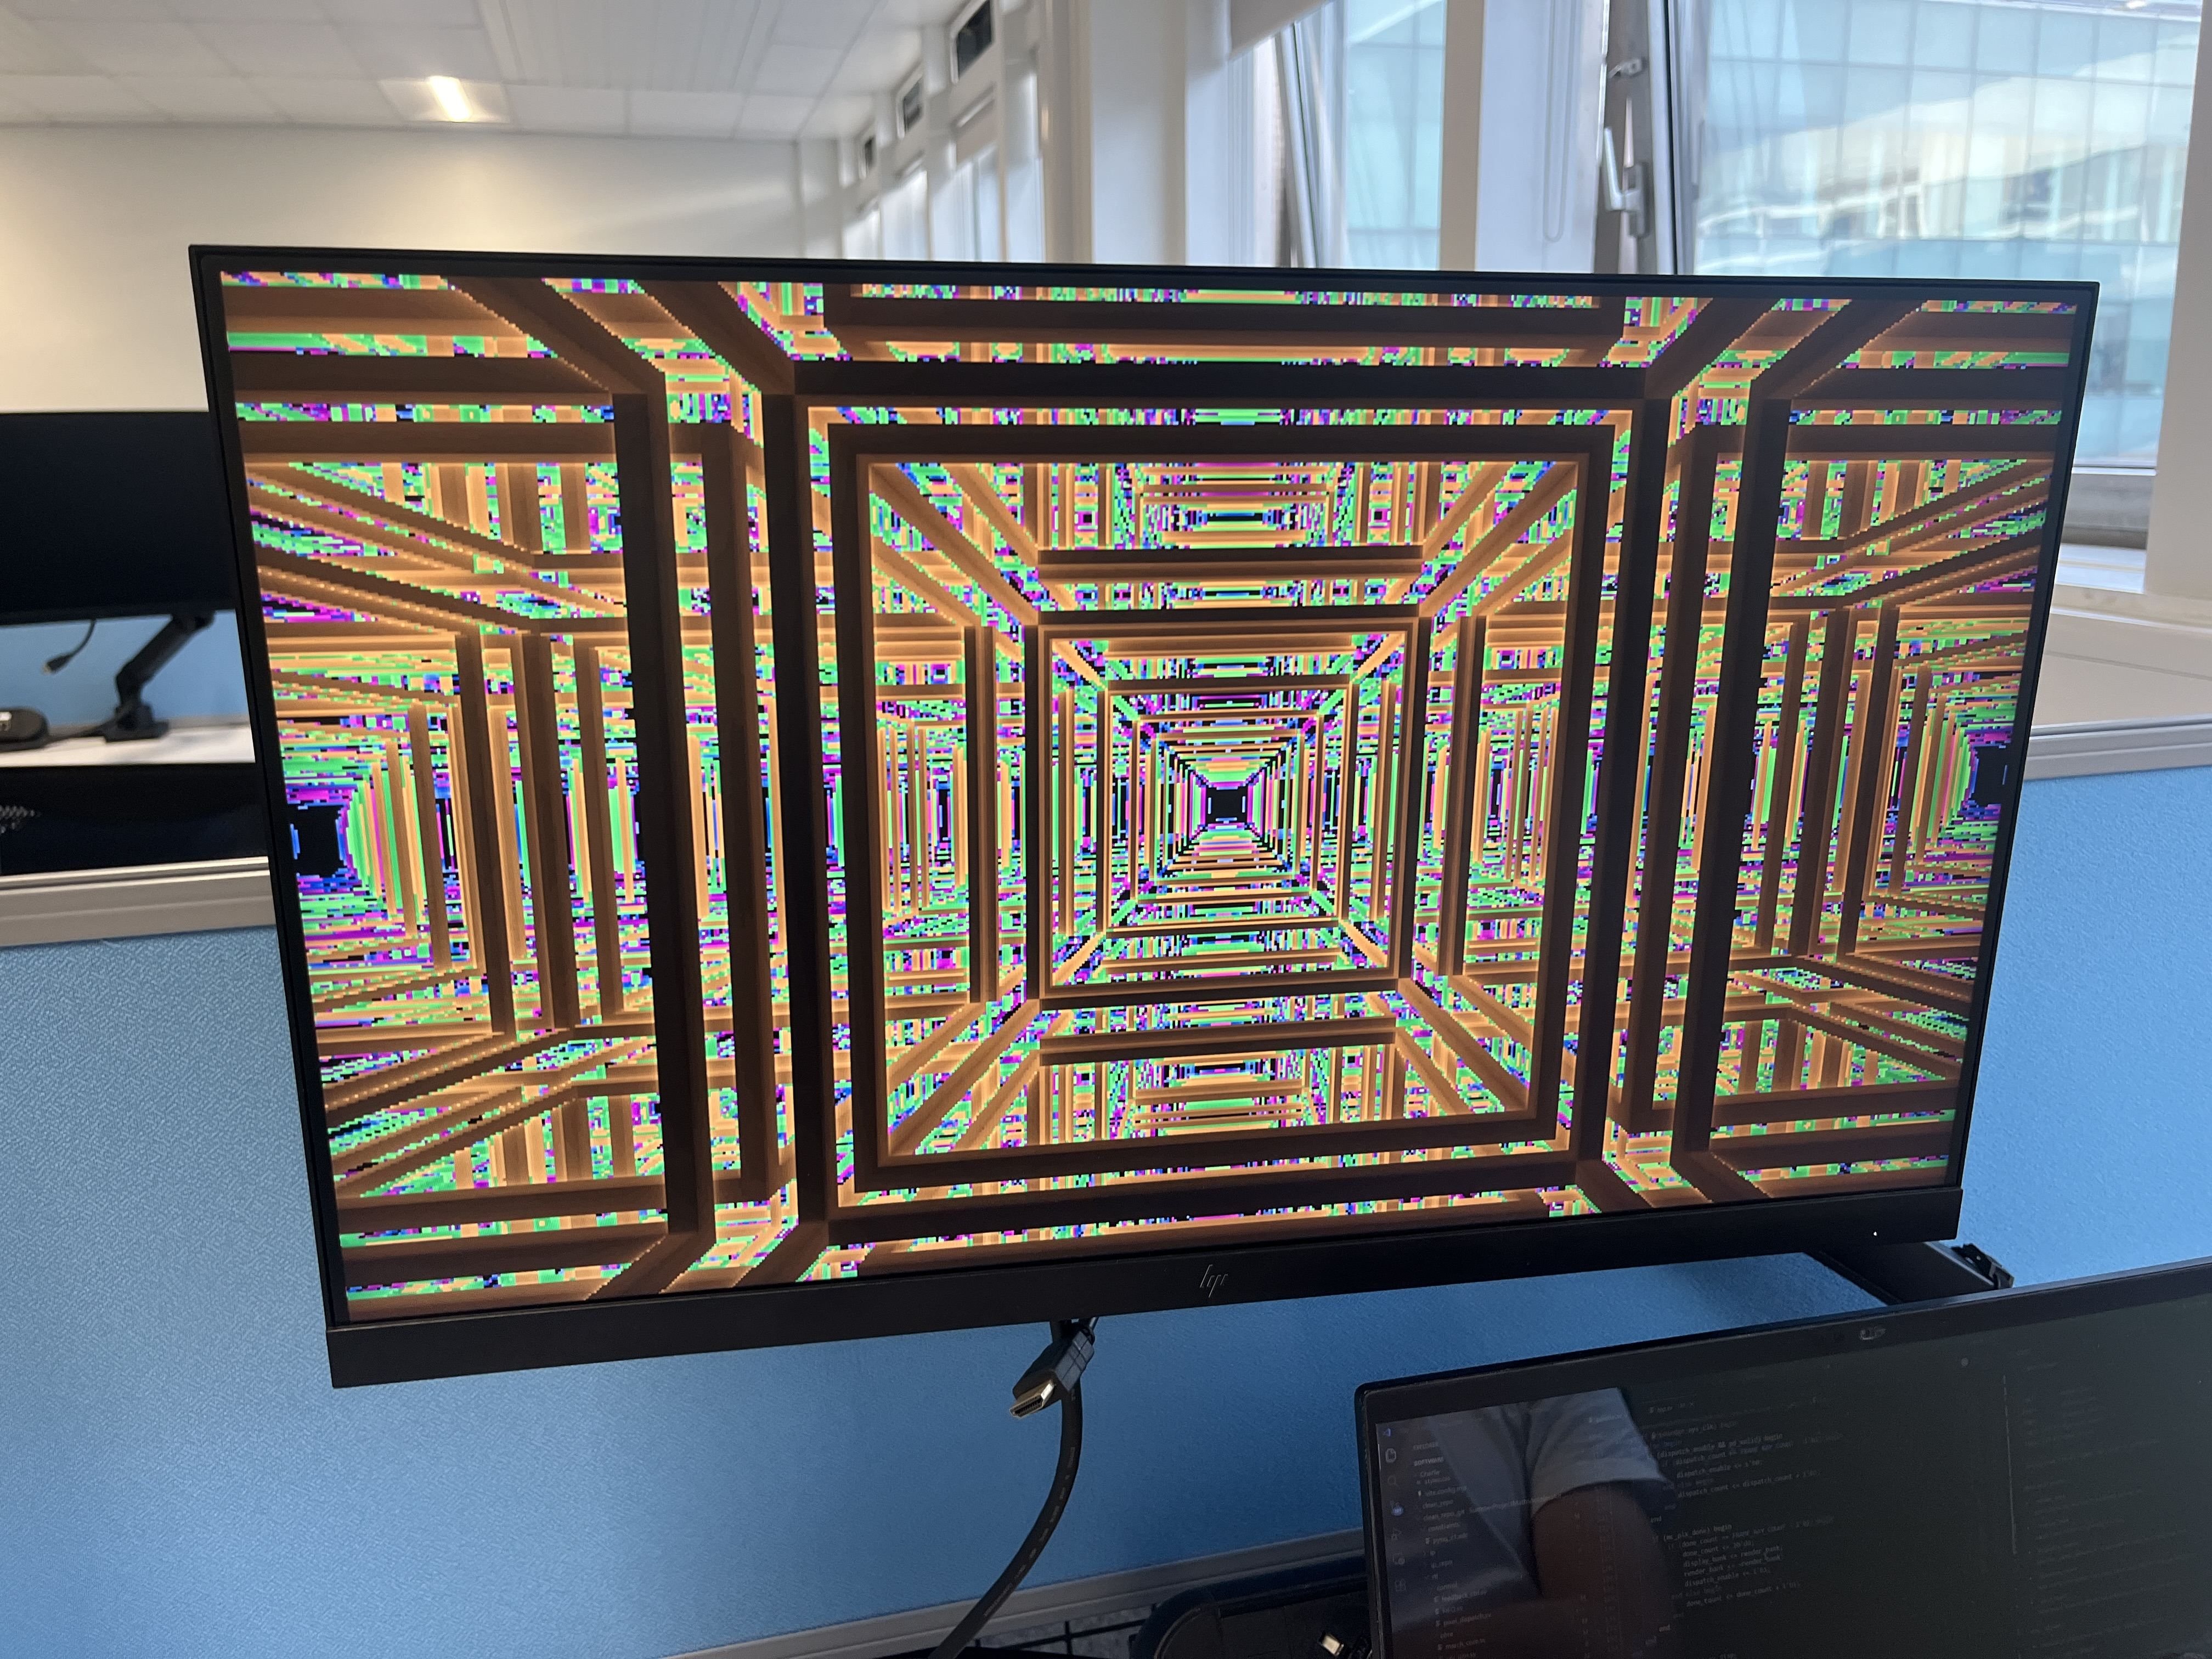
\includegraphics[width=\textwidth]{imgs/initial_scaffold.JPG}
        \vspace{-0.2cm}
        \captionof{figure}{First render of scaffold on screen, no split screen yet - no VR.}
        \label{fig:sphere_sdf_infinite}
    \end{minipage}%
    \hfill % Pushes the second minipage cleanly to the right margin
    \begin{minipage}{0.48\textwidth}
        \centering
        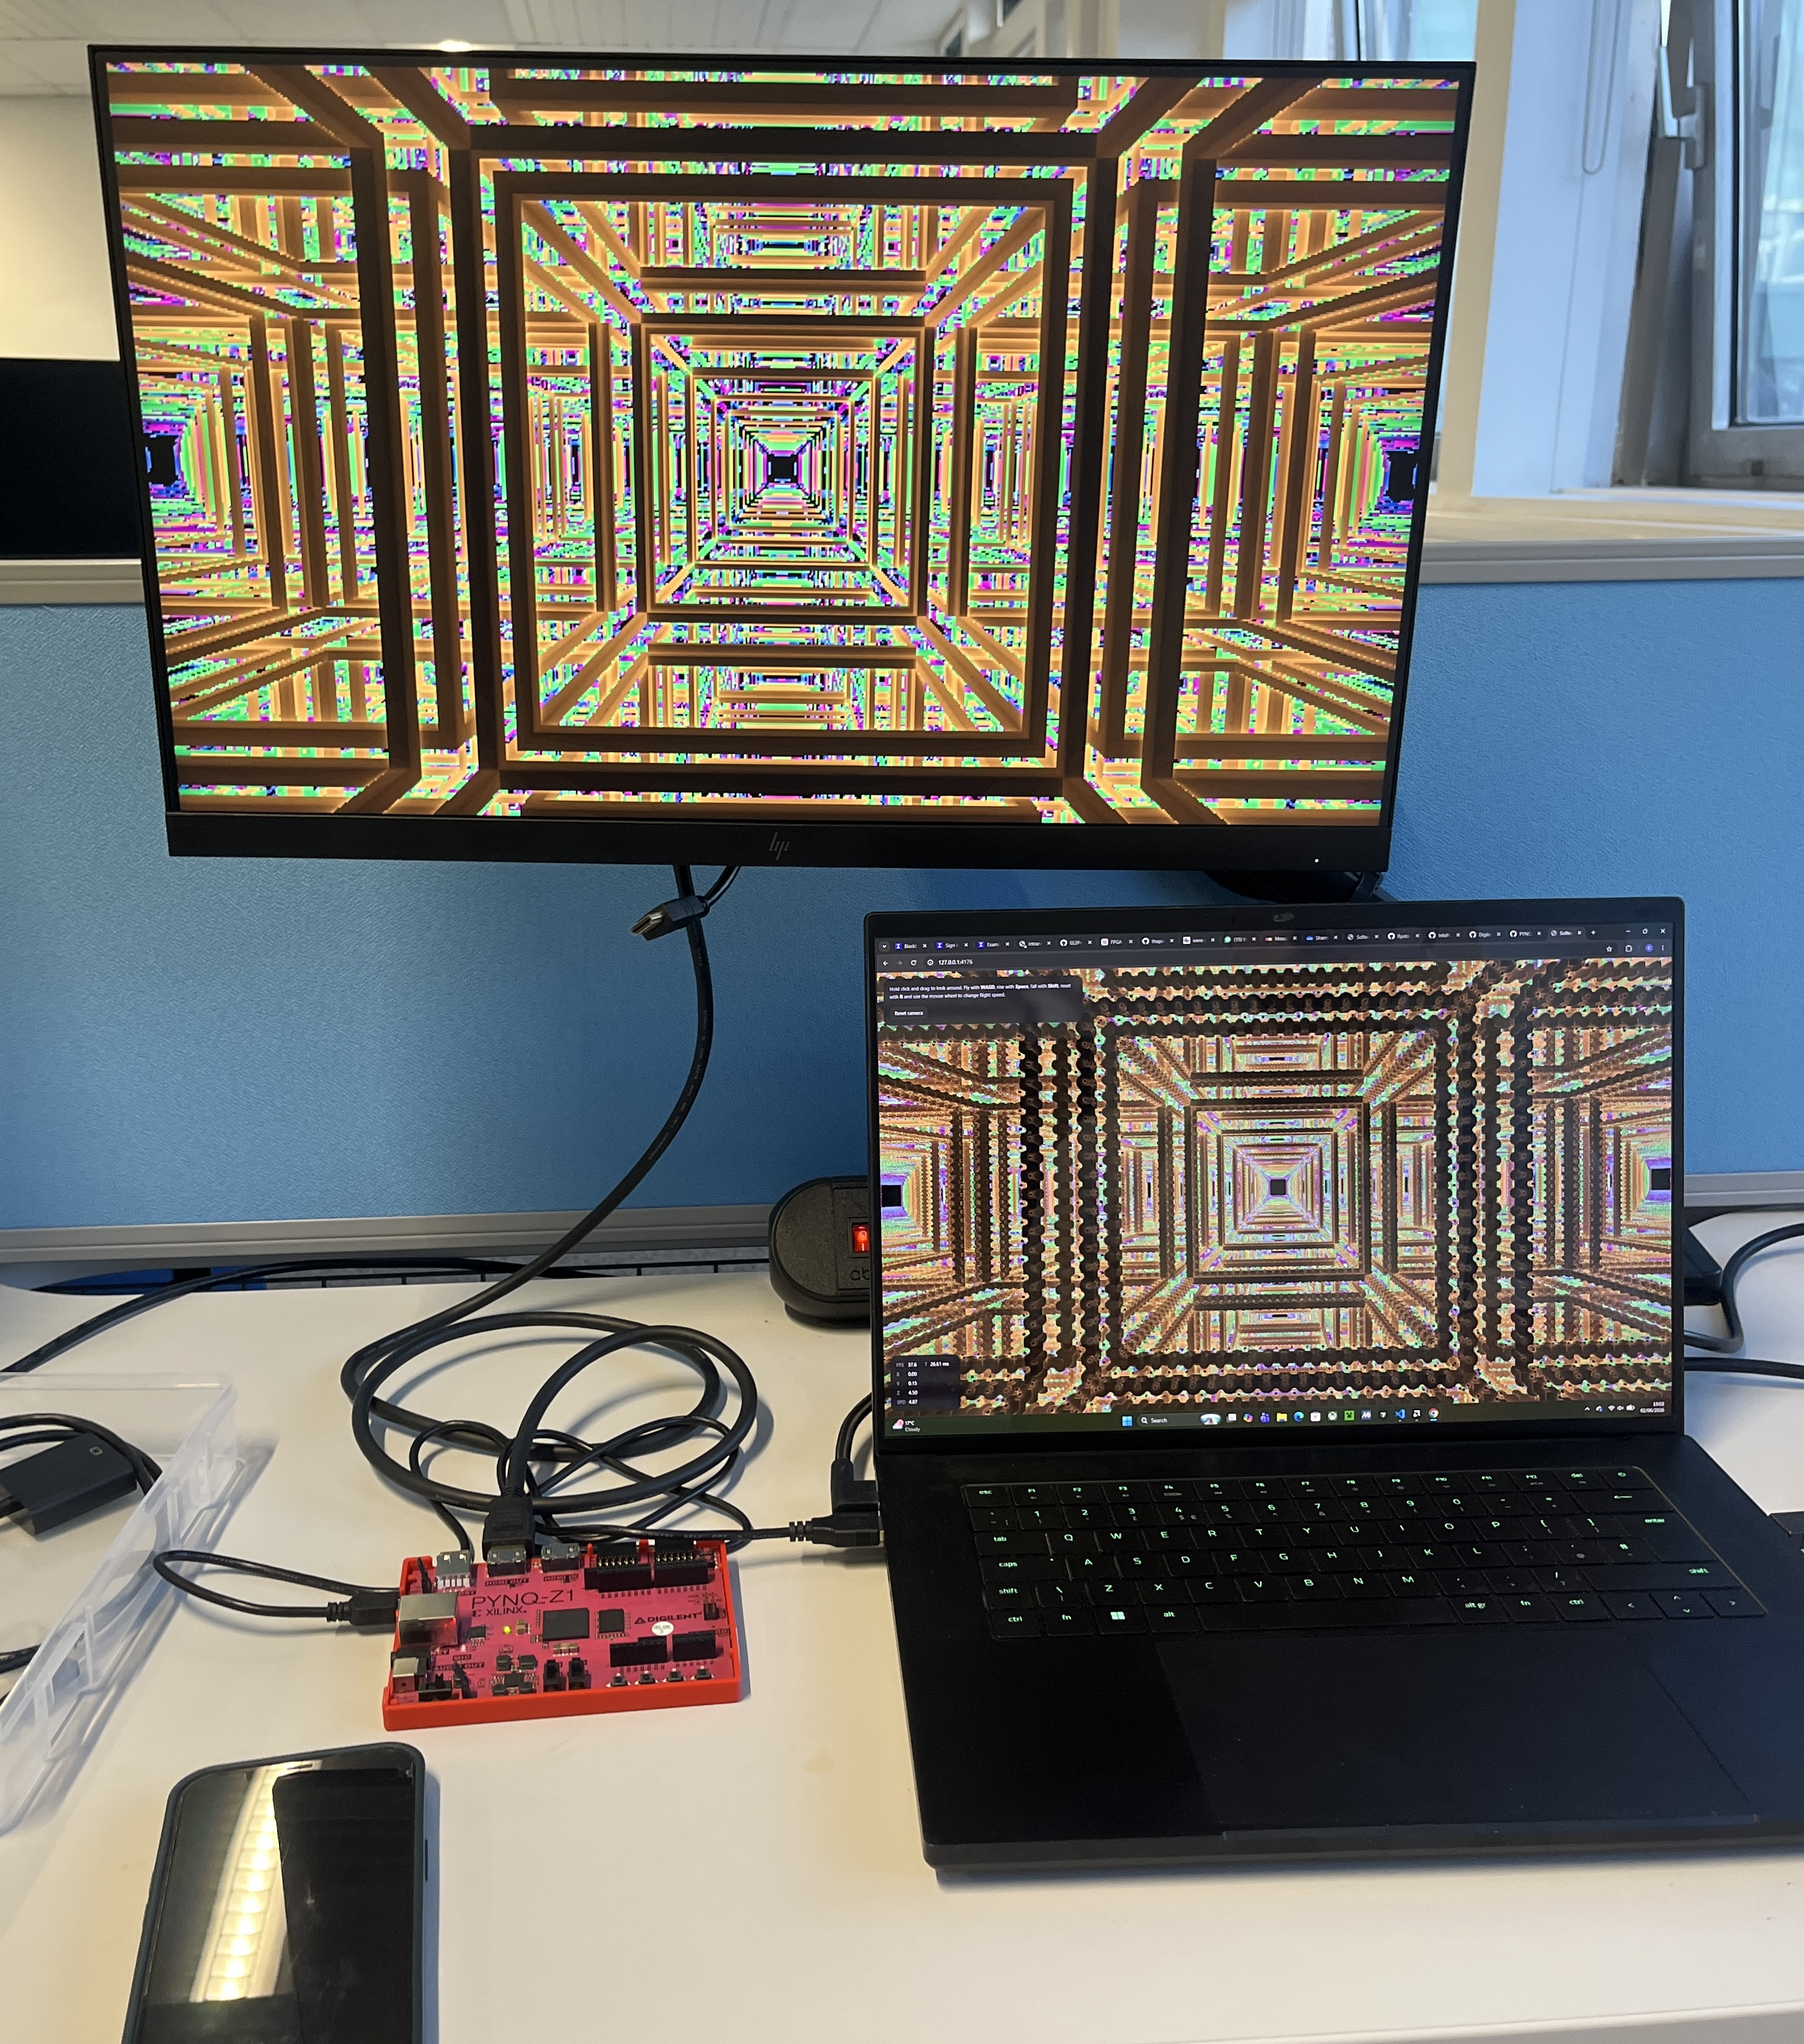
\includegraphics[width=\textwidth]{imgs/initial_scaffold2.jpg}
        \vspace{-0.2cm}
        \captionof{figure}{GSLS Version next to FPGA version, no movement yet}
        \label{fig:hardware_matrix_display}
    \end{minipage}
\end{center}
% ----------------------------------------------------------------

\subsection{Reciprocal and Division}

\paragraph{Reciprocal - \code{fp\_inverse.sv}.}
Newton-Raphson on $f(x) = 1/x - b$ gives $x_{n+1} = x_n(2 - bx_n)$, which
converges quadratically ($e_{n+1} = e_n^2$). The initial estimate flips the
exponent field, giving $bx_0 \in [1,2)$ and guaranteed convergence. Three
iterations of 12 cycles each reduce error from $\sim$25\% to $\sim$0.0015\%;
total latency: 36 cycles.

\paragraph{Division - \code{fp\_division.sv}.}
$a/b$ is computed as $a \times \text{fp\_inverse}(b)$, with $a$ delayed 36
cycles through \code{state\_pipe} to arrive cycle-aligned. Total latency: 40
cycles.

\subsection{Modulus - \code{fp\_modulus.sv}}

$a \bmod b = a - b\cdot\lfloor a/b\rfloor$, where \code{fp\_floor} is purely
combinational, masking fractional mantissa bits by exponent. The full chain -
division (40) $\to$ floor (0) $\to$ multiply (4) $\to$ subtract (4) - gives
52 cycles total, the most expensive primitive in the library and the dominant
term in SDF evaluation latency for space-repetition scenes.

\subsection{Pipeline Synchronisation - \code{state\_pipe}}

When two computation chains of unequal length must produce cycle-aligned
outputs, \code{state\_pipe} delays the shorter chain. It is a parameterised
shift register synthesised by Vivado as SRLs rather than flip-flop chains,
significantly reducing flip-flop usage. Misalignment by even one cycle produces
completely corrupted renders with no obvious visual diagnostic.

\subsection{Matrix-Vector Product - \code{fp\_mul\_vec3\_mat33.sv}}

Nine parallel \code{fp\_mul} instances compute all products of the $3\times3$
lookat matrix simultaneously in 4 cycles; three pairs of \code{fp\_add}
accumulate row sums in 4 more cycles. Total latency: 8 cycles, with no internal
synchronisation delay lines required, as all nine multiplies share the same
input register.

\FloatBarrier


% ===============================================================
\section{Ray Generation}
% ===============================================================

\subsection{Purpose and Design}
\code{ray\_gen.sv} is a fully pipeined, non-stalling module that converts pixel coordinates into world-space unit ray. It accepts one pixel per clock cycle  and produces the corresponding ray 45 cycles later.

\code{ray\_gen.sv} transforms a pixel coordinate $(p_x, p_y)$ and the camera
lookat matrix into a normalised world-space ray direction. The pixel coordinate
is first converted from screen space to normalised device coordinates (NDC),
scaled to a $[-1, 1]^2$ viewport, then transformed by the $3 \times 3$ lookat
matrix to produce the world-space direction. Coordinates are doubled
(working at $2\times$ integer resolution) to avoid non-integer pixel centres,
where the true centre of a $1280 \times 720$ display falls at $x = 639.5$,
represented exactly in $2\times$ space. The FOV is controlled by
\code{FOV\_Z\_CONST}, encoding the virtual focal length. At $1024\times600$ the
constant is set to \texttt{27'h221A000} ($\approx 83.3^\circ$ horizontal FOV). 

The conversion from integer pixel coordinates to FP27 is done by a fully
unrolled combinational function \code{fp\_int2fp} inside the module, avoiding
an extra pipeline stage.

Three SystemVerilog testbenches provide 47 tests with zero failures: \texttt{tb\_axi\_camera\_regs.sv} (16 tests, register write/readback and commit atomicity), \texttt{tb\_ray\_gen.sv} (17 tests, centre and off-axis pixel directions), and \texttt{tb\_fp\_ops.sv} (14 tests, FP27 arithmetic including $1/\sqrt{4.0} = 0.4991$, confirming Newton--Raphson convergence).

\subsection{AXI-Lite Camera Interface}

The PS communicates camera parameters to the PL through an AXI-Lite register
file at base address \texttt{0x43C00000}. The register map is:

\begin{table}[htbp]
\centering
\small
\caption{AXI-Lite camera register map}
\label{tab:axi_regs}
{\renewcommand{\arraystretch}{1.3}
\begin{tabular}{cll}
\toprule
\textbf{Register offset} & \textbf{Content} & \textbf{Width} \\
\midrule
\texttt{0x00}--\texttt{0x20} & Lookat matrix rows 0--8 & 9 $\times$ FP27 \\
\texttt{0x24}--\texttt{0x2C} & Camera origin $x, y, z$ & 3 $\times$ FP27 \\
\texttt{0x30}--\texttt{0x4C} & SDF parameters 0--7     & 8 $\times$ FP27 \\
\texttt{0x50} & Camera commit (write 1 to latch)       & 1-bit \\
\bottomrule
\end{tabular}}
\end{table}

\FloatBarrier

The commit register prevents the pipeline from reading a partially updated
camera matrix. The PS writes all 12 parameters then pulses the commit register,
atomically latching them into the registers visible to the PL.

\code{ray\_gen} has a fixed latency of 48 clock cycles, determined by the depth
of the \code{fp\_mul\_vec3\_mat33} chain (8 cycles) plus pipeline register stages
that prevent the module from becoming the critical path.


\FloatBarrier


% ===============================================================
\section{Ray Marcher Core}
\label{sec:marchcore}
% ===============================================================

\subsection{Architecture and Pipeline Stages}

\code{march\_core.sv} is the computational heart of the renderer. It receives
a pixel payload (coordinates, ray position, ray direction, iteration count,
accumulated distance) and performs one sphere-tracing step: evaluate the SDF
at the current position, advance the ray by the returned distance, and either
terminate the ray or return it to the feedback controller for another iteration.

The core is a three-stage fully pipelined architecture with per-iteration latency
of 163 clock cycles:

\begin{enumerate}
    \item \textbf{Ray generation (48 cycles).} On iteration 0, \code{ray\_gen}
    computes the world-space ray direction from the pixel coordinate and lookat
    matrix. On subsequent iterations this stage is bypassed --- the direction and
    position carried from the previous feedback output are used directly. A
    combinational mux selects between the two:
\begin{lstlisting}[language=Verilog]
localparam RG_LAT  = 48;
localparam SDF_LAT = 107;
localparam STEP_LAT = 8;

wire [26:0] s1_pos_x = (d1_iter == 8'd0) ? rg_orig[0] : d1_pos_x;
wire [26:0] s1_dir_x = (d1_iter == 8'd0) ? rg_dir[0]  : d1_dir_x;
\end{lstlisting}
    All feedback signals are delayed by exactly \texttt{RG\_LAT = 48} cycles
    using \code{state\_pipe} instances so they arrive at this mux simultaneously
    with the ray generation output.

    \item \textbf{SDF evaluation (107 cycles).} The current position
    $(p_x, p_y, p_z)$ is passed to the SDF module, which returns the signed
    distance to the nearest surface. For scenes using space repetition, the three
    FP modulus operations account for $3 \times 52$ cycles, but the modulus chains
    are partially parallel and the overall SDF latency for the scaffold scene is
    107 cycles. All position, direction, iteration count, and pixel ID signals
    are delayed through \code{state\_pipe} instances of depth 107 so they arrive
    cycle-aligned with the SDF output.

    \item \textbf{Step and hit detection (8 cycles).} The sphere-tracing step
    advances the ray position by the SDF distance:
    \[
        \mathbf{p}_{n+1} = \mathbf{p}_n + d_{\text{SDF}} \cdot \hat{\mathbf{r}}
    \]
    Three parallel \code{fp\_mul} instances compute $d \cdot r_x$, $d \cdot r_y$,
    $d \cdot r_z$, followed by three \code{fp\_add} instances, for 8 cycles total.
    Hit and miss conditions are evaluated combinationally:
\begin{lstlisting}[language=Verilog]
localparam [26:0] HIT_THRESH = {1'b0, 8'd117, 18'h01893}; // ~0.001
localparam        MAX_ITER   = 128;

wire hit_comb  = d3_valid & (d3_dist[26] | (d3_dist < HIT_THRESH));
wire miss_comb = d3_valid & (d3_iter >= MAX_ITER);
wire done_comb = hit_comb | miss_comb;
\end{lstlisting}

    \code{HIT\_THRESH} encodes $\approx 10^{-3}$: exponent field $117 = 127 - 10$
    gives $2^{-10}$; mantissa $\texttt{0x01893} \approx 0.024$; value
    $(1.024) \times 2^{-10} \approx 0.001$. A ray is also considered to have hit
    if the SDF returns a negative value (sign bit set), indicating the ray
    overshot the surface. \code{MAX\_ITER = 128} limits total depth; rays that
    never converge terminate and are coloured by their accumulated travel distance.
\end{enumerate}

Each cycle the core asserts either \code{pix\_done} (ray terminated; iteration count forwarded to the fog LUT for RGB mapping) or \code{fb\_valid} (ray continues; updated position and direction returned to \code{feedback\_ctrl}). Both paths are registered with no combinational output.

\subsection{Space Repetition in the Scaffold SDF}

The scaffold scene tiles infinite space by replacing the marched position with
its modulo equivalent in a canonical cell before SDF evaluation:

\begin{lstlisting}[language=Verilog]
assign cell_sz = sdf_params[0];  // bass FFT energy -> AXI-Lite reg
fp_modulus inst_x(.a(px), .b(cell_sz), .rem(rep_px));
fp_modulus inst_y(.a(py), .b(cell_sz), .rem(rep_py));
fp_modulus inst_z(.a(pz), .b(cell_sz), .rem(rep_pz));
\end{lstlisting}

\begin{figure}[h!]
\centering
\begin{tikzpicture}[
  arr/.style={-{Stealth[length=5pt]}, thick},
  cell/.style={draw=gray!60, fill=gray!10, minimum width=2cm, minimum height=2cm},
  canon/.style={draw=ImperialBlue, fill=blue!8, minimum width=2cm, minimum height=2cm, line width=1.2pt},
  obj/.style={circle, draw=red!70!black, fill=red!20, minimum size=0.55cm, inner sep=0pt},
  lbl/.style={font=\small},
]

%% --- tiling cells along x ---
\foreach \i/\col in {0/gray!10, 1/gray!10, 2/blue!8, 3/gray!10, 4/gray!10} {
  \pgfmathsetmacro\xi{\i*2.2}
  \draw[draw=gray!60, fill=\col, line width={\i==2 ? 1.2pt : 0.6pt}]
    (\xi, 0) rectangle ++(2.0, 2.0);
  % object ghost in each cell
  \node[obj, opacity={\i==2 ? 1 : 0.25}] at (\xi+1.0, 1.0) {};
}

%% canonical cell label
\node[font=\small\bfseries, color=ImperialBlue] at (2*2.2+1.0, 2.35) {canonical cell};

%% cell_sz brace
\draw[decorate, decoration={brace, amplitude=4pt, mirror}]
  (0, -0.25) -- (2.0, -0.25) node[midway, below=-15pt, font=\scriptsize] {\texttt{cell\_sz}};

%% camera
\node[draw, fill=yellow!20, minimum width=0.7cm, minimum height=0.5cm, font=\scriptsize] (cam) at (-1.8, 0.6) {cam};

%% ray line from camera across cells, hitting obj in cell 2
\draw[arr, color=black!70, dashed] (cam.east) -- (2*2.2+1.0, 1.0);

%% sample points on the ray
\foreach \xi/\yi in {0.5/0.72, 1.3/0.82, 2.8/0.90, 4.5/0.97} {
  \fill[black!50] (\xi, \yi) circle (1.8pt);
}

%% fmod arrow from sample in cell 0 down to canonical
\draw[arr, color=ImperialBlue, bend right=20]
  (0.5, 0.72) to node[lbl, left, xshift=-2pt]{\texttt{fmod(p,c)}} (2*2.2+0.5, 0.72);

%% hit annotation
\node[font=\scriptsize, color=red!70!black] at (2*2.2+1.0, 0.55) {SDF $<$ thresh};
\draw[-{Stealth[length=4pt]}, red!70!black] (2*2.2+1.0, 0.65) -- (2*2.2+1.0+0.25, 0.88);

%% miss annotation (cell 0)
\node[font=\scriptsize, color=black!50, align=center] at (1.0, -0.55) {SDF $\gg$ 0\\(step forward)};

\end{tikzpicture}
\caption{Space repetition via \texttt{fp\_modulus}: the ray position $\mathbf{p}$ at each march step is wrapped into the canonical cell by \texttt{fmod(p, cell\_sz)} before SDF evaluation. The infinite tiling is implicit - only one cell's SDF is ever evaluated. Bass FFT energy sets \texttt{cell\_sz} at runtime, expanding or compressing the tile density, effectively compressing and dilating space.}
\label{fig:space-rep}
\end{figure}

The key insight is that the SDF of an infinite tiling equals the SDF of a single
canonical cell evaluated at the wrapped coordinate. This is valid provided the
cell half-width exceeds the geometry's maximum extent. The cell size is written
from the PS each audio block, making the tiling density a live parameter driven
by bass energy. The \code{fp\_modulus} latency of 52 cycles dominates SDF
evaluation and drives the \code{SDF\_LAT = 107} parameter in \code{march\_core}.
Note that it is important to leave a spacing of minimum 0.1 units between cell size and object size/radius, as the Newton Raphson iterations for modulo, by nature inexact, can cause imprecisions and at worst bleeding (ie, geometry is lost as coloring no longer corresponds to due cell).

Space repetition tooks days to implement. The Newton Raphson logic is not easy and floor function in FP27 is quite difficult to understand (though basic in bit masking technique). Before infinite tiling, a Look Up Table approach was used to determine canonical positions at certain points. This caused the world to have borders, leading to interesting landscapes, see below!
\begin{figure}[htbp]
    \centering
    \begin{minipage}[b]{0.48\textwidth}
        \centering
        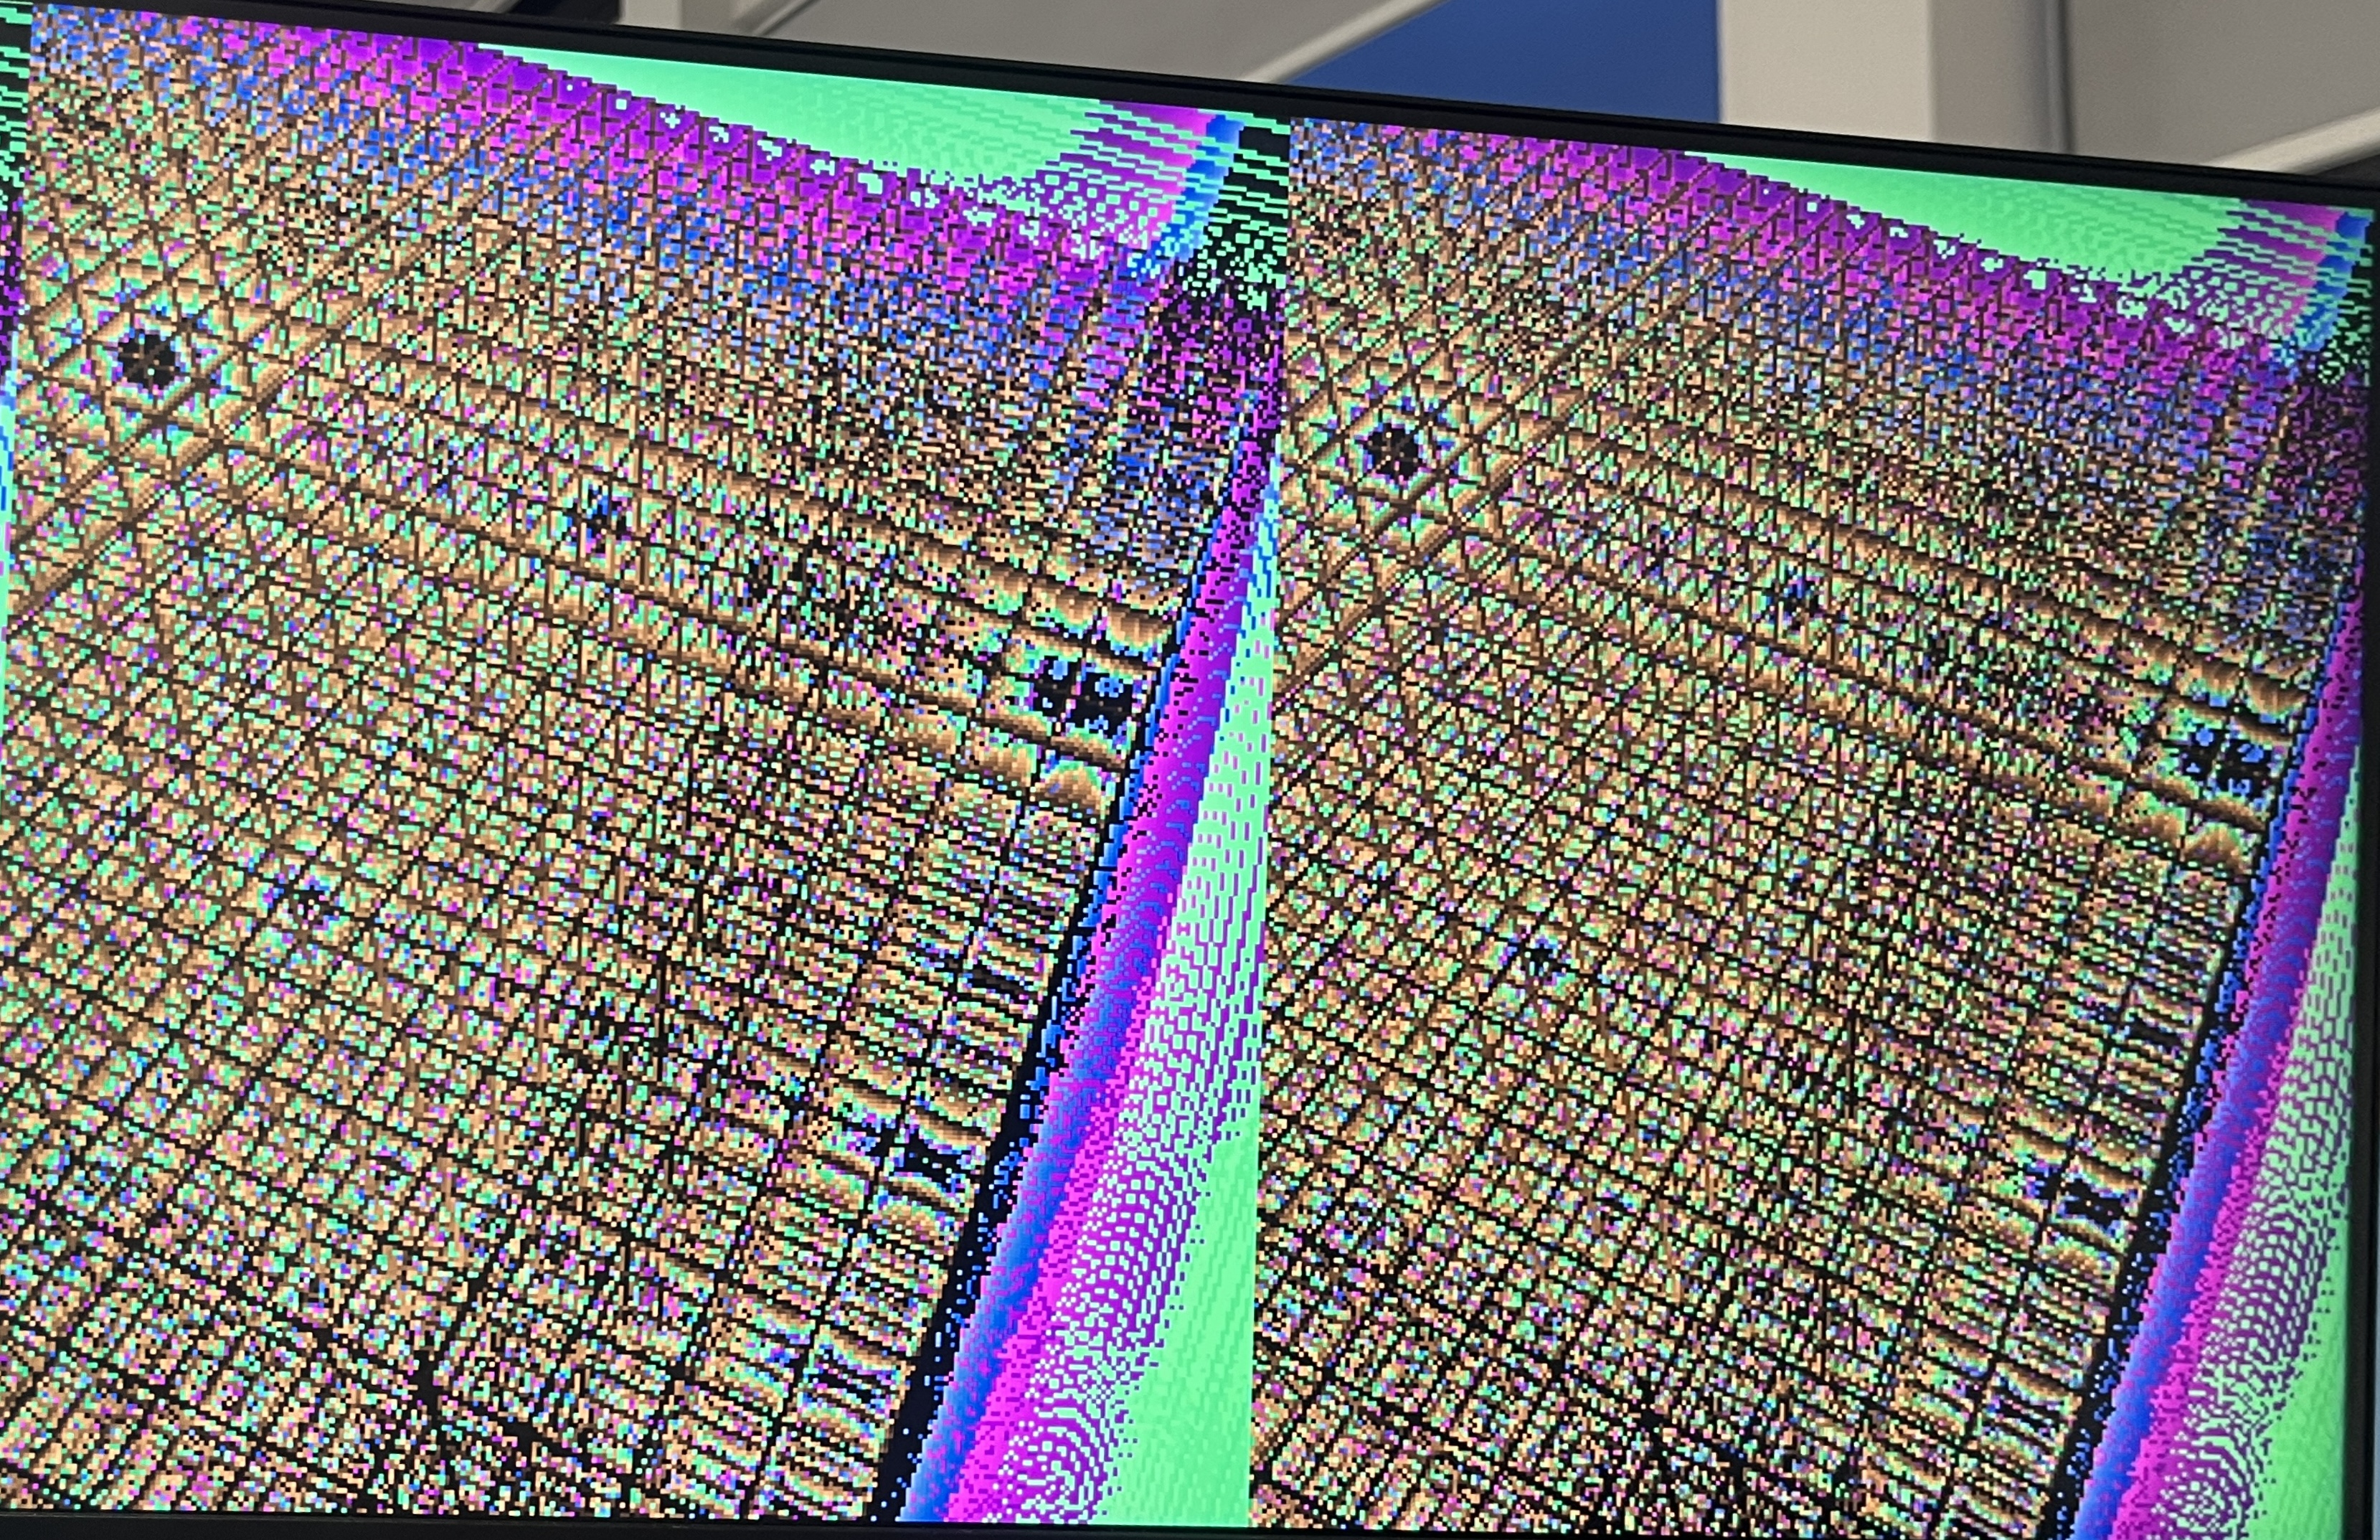
\includegraphics[width=\textwidth]{imgs/scaffold_borders1.jpg}
        \label{fig:image1}
    \end{minipage}
    \hfill
    \begin{minipage}[b]{0.48\textwidth}
        \centering
        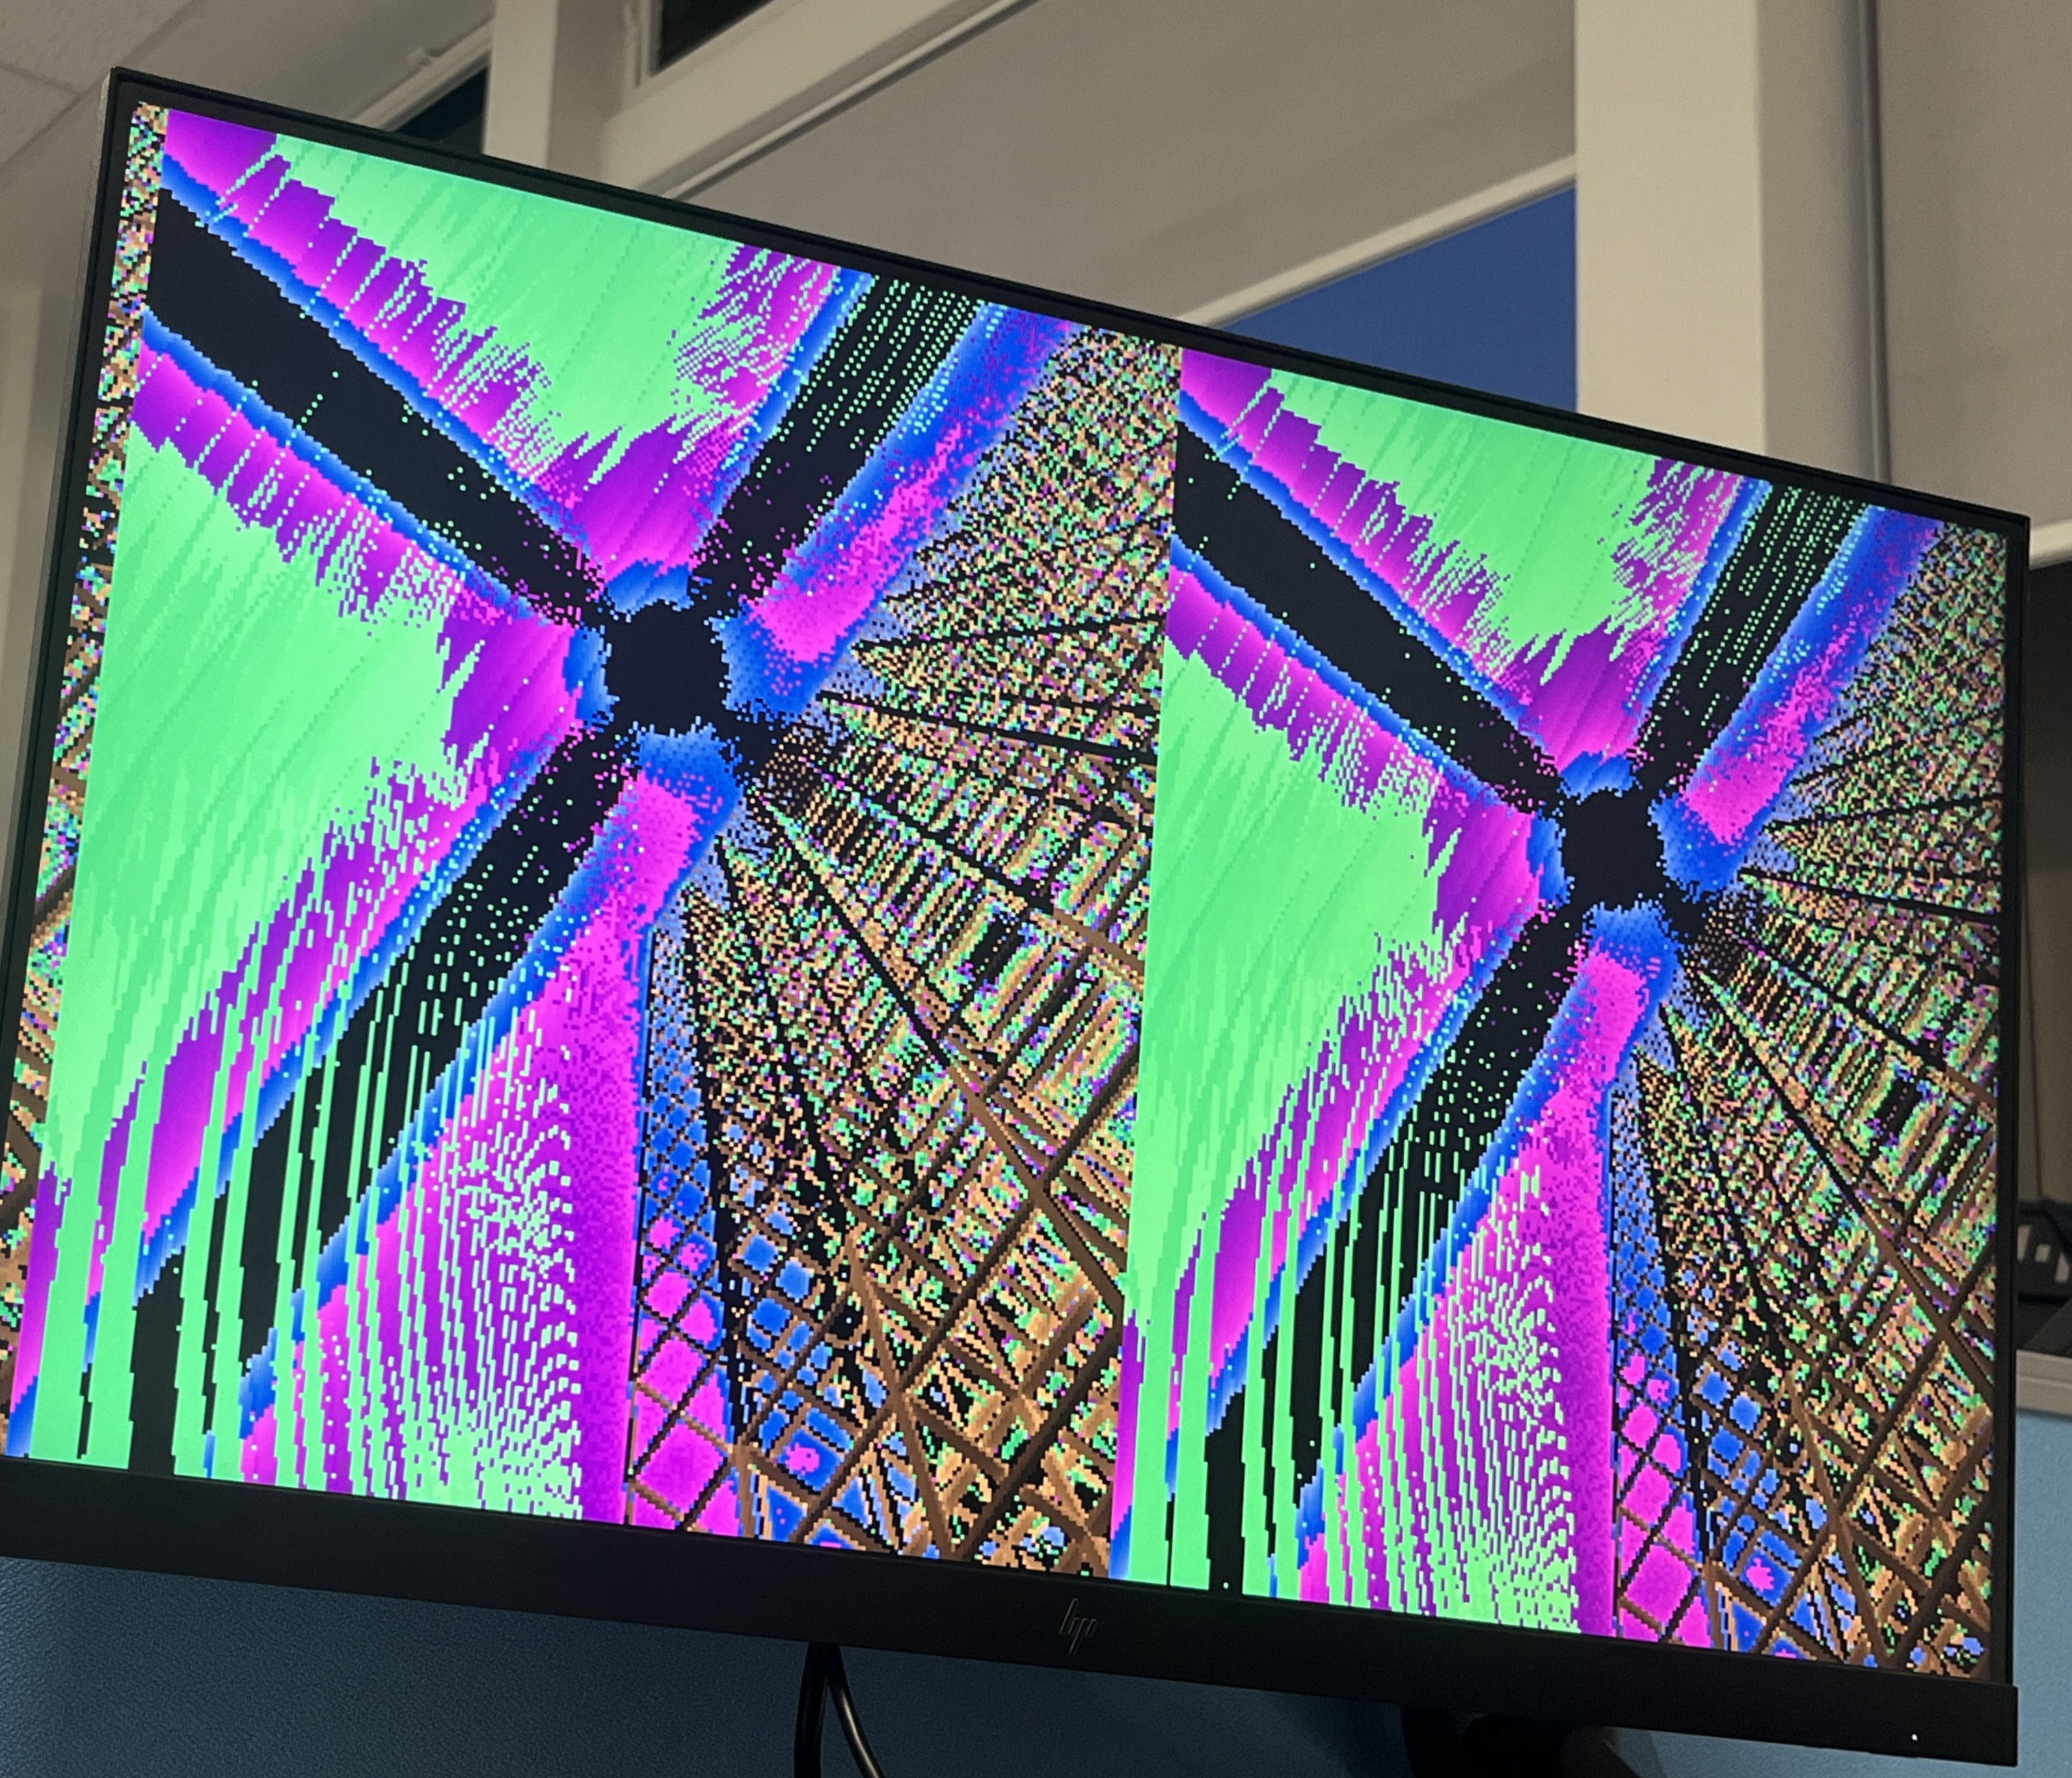
\includegraphics[width=\textwidth]{imgs/scaffold_borders2.jpg}
        \label{fig:image1000}
    \end{minipage}
    \caption{World edges visible, scaffold signed distance repetition suddenly stops.
    The exterior colouring is due to the periodic nature of palette.sv coloring.}
\end{figure}

\FloatBarrier


% ===============================================================
\section{Pixel Dispatch and Feedback Scheduling}
% ===============================================================

\subsection{Introduction}

The pixel pipelining comprises several hardware components ranging from initial
ray generation to final HDMI output. To ensure a controlled and ordered flow of
pixels, the infrastructure relies upon a coordinated traffic management layer.

\subsection{\code{pixel\_dispatch.sv}}

The first and most crucial component is \code{pixel\_dispatch}, which executes a
continuous raster scan of all on-screen pixels to guarantee deterministic
throughput. In addition to the coordinate stream, this module assigns a tracking
index (\code{pix\_id}) to each payload. The tag travels through the pipeline with
the ray data and allows downstream modules to map returning pixels to their
specific memory slots without losing coordinate context.

Once a valid pixel is obtained from the raster scan, \code{pixel\_dispatch}
samples the synchronous \code{pipeline\_ready} signal asserted by
\code{feedback\_ctrl}. A high signal invites the dispatcher to advance its
raster count and stream Cartesian coordinates and the 20-bit pixel ID to the
ray generation module. A low signal indicates the feedback loop is under
execution; \code{pixel\_dispatch} applies backpressure by stalling its counter,
preventing FIFO overflow and protecting the feedback loop against structural
deadlock.

\subsection{\code{feedback\_ctrl.sv}}

\code{feedback\_ctrl} arbitrates between new coordinates from
\code{pixel\_dispatch} and active rays returning from the march core, mirroring
a multiplexer. Since the ray generator and march core are deep pipelined
architectures, many pixels are simultaneously in-flight. Rays requiring
additional iterations must be routed back to the front of the pipeline via a
FIFO storage buffer.

When the FIFO is non-empty, \code{feedback\_ctrl} asserts \code{read\_enable},
passes the stored payload to the ray generator, and sends a backpressure signal
to \code{pixel\_dispatch} to stall the raster counter. When the FIFO is empty,
\code{pixel\_dispatch} advances and a new pixel enters the pipeline directly.
The feedback loop is always prioritised to prevent structural deadlock.

\subsection{\code{FIFO.sv}}

\code{FIFO.sv} implements a synchronous dual-port memory array with read and
write pointers. The payload width was carefully compressed to 190 bits per entry.
Numerical analysis of the pipeline gives a maximum in-flight pixel count of 103
cycles (48 ray gen + 55 march). A 128-entry deep FIFO provides 24.3\% headroom,
accommodating transient stalls without interfering with active pixels.

\subsection{\code{fb\_write.sv}}

\code{fb\_write} extracts the iteration count from completed rays, raises
\code{bram\_we}, and maps the \code{pix\_id} to the correct framebuffer address.
The framebuffer is a dual-port BRAM: one port handles write operations from
\code{fb\_write}, the other is dedicated to HDMI scan-out, bridging the rendering
and pixel clock domains without metastability.

\subsection{Verification}

\begin{table}[htbp]
\centering
\small
\caption{Pixel management verification results}
\label{tab:pixel_verification}
{\renewcommand{\arraystretch}{1.3}
\begin{tabular}{llp{6.5cm}}
\toprule
\textbf{Testbench} & \textbf{Module} & \textbf{Result} \\
\midrule
\code{pixel\_dispatch\_tb.sv} & \code{pixel\_dispatch} & PASS: all 921,600 pixels emitted exactly once \\
\code{feedback\_ctrl\_tb.sv}  & \code{feedback\_ctrl}  & PASS: FIFO stall and priority arbitration correct \\
\code{fb\_write\_tb.sv}       & \code{fb\_write}       & PASS: \code{bram\_we} and address on every done pixel \\
\code{integration\_tb.sv}     & Full interface         & PASS: $640\times360$ screen with zero duplicates \\
\bottomrule
\end{tabular}}
\end{table}

\FloatBarrier

\section{Timing Closure: 40Mhz to 200Mhz}

  The initial design ran at 40\,MHz with WNS\,=\,$+$16.3\,ns. Reaching                                                      
  200\,MHz required ten iterations of identifying and breaking critical paths
  from post-route timing reports:                                                                                           
                  
  \begin{itemize}
    \item \textbf{fp\_add casex priority encoder:} The stage-4 leading-one
    scan synthesised to a ripple chain of $\sim$20 LUT levels ($\sim$8\,ns).
    Replacing it with a flat \texttt{casex} enumerating all 20 shift amounts
    reduced the depth to $\sim$5 LUT levels.

    \item \textbf{fp\_mul DSP targeting and register insertion:} The
    19$\times$19 mantissa multiply used one DSP48E1 plus a 6-level fabric
    carry chain (5.7\,ns). Adding \texttt{(* use\_dsp = "yes" *)} eliminated
    the fabric path entirely, reducing delay to 1.9\,ns.

    \item \textbf{Pipeline register insertions:} Cascaded \texttt{fp\_min}
    comparators in \texttt{scene\_sdf} formed an 11-level, 7.1\,ns path;
    a register inserted between them halved the depth (\texttt{SDF\_LAT}
    incremented by 1 to compensate).

    \item \textbf{FIFO depth reduction and XDC constraints:} The DDR write
    FIFO at \texttt{FIFO\_DEPTH\,=\,4096} required 2880 RAM64E cells spanning
    34 fabric columns (WNS\,=\,$-$0.312\,ns). Reducing depth to 1024 collapsed
    the 64:1 mux to 16:1, cutting routing delay to 0.7\,ns. A pblock
    (\texttt{SLICE\_X0Y0:SLICE\_X69Y149}) confined \texttt{march\_core} to a
    contiguous region, and \texttt{(* max\_fanout\,=\,16 *)} was applied to
    the write-enable bus.

    \item \textbf{Pipeline resynchronisation:} When \texttt{fp\_mul} grew from
    3 to 4 cycles and \texttt{fp\_isqrt} from 10 to 16 cycles, flashing
    artefacts appeared on hardware. The root cause was \texttt{march\_core}
    pairing the SDF distance evaluated for ray $N$ with the position of ray
    $N+4$. All companion \texttt{state\_pipe} depths were recalculated to
    restore exact alignment.
  \end{itemize}

  The final 200\,MHz implementation reports WNS\,=\,0.000\,ns,
  TNS\,=\,0.000\,ns, and 0 failing endpoints.

  \begin{table}[h!]
  \centering
  \caption{Timing at each frequency milestone}
  \begin{tabular}{lrrrr}
  \hline
  \textbf{Milestone} & \textbf{Freq} & \textbf{Period} & \textbf{WNS} & \textbf{Failing} \\
  \hline
  Baseline (bring-up fixes) & 40\,MHz  & 25.0\,ns & $+$16.300\,ns & 0 \\
  Milestone 1               & 100\,MHz & 10.0\,ns & $+$0.067\,ns  & 0 \\
  Milestone 2               & 150\,MHz &  6.7\,ns & $+$0.145\,ns  & 0 \\
  Milestone 3               & 200\,MHz &  5.0\,ns & $+$0.000\,ns  & 0 \\
  \hline
  \end{tabular}
  \end{table}

  \begin{table}[h!]
  \centering
  \caption{150\,MHz iterative closure}
  \begin{tabular}{lrrr}
  \hline
  \textbf{Change applied} & \textbf{WNS (ns)} & \textbf{TNS (ns)} & \textbf{Failing} \\
  \hline
  Initial 150\,MHz                     & $-$2.514 & $-$2243   & 2385 \\
  fp\_add casex + parallel subtractors & $-$1.738 & $-$1125   & 1983 \\
  Pblock + impl strategy               & $-$0.681 & $-$173    &  614 \\
  scene\_sdf pipeline register         & $-$0.629 & $-$1098   &  120 \\
  fp\_mul stage split + DSP forcing    & $-$0.364 & $-$196    &   90 \\
  sdf\_term pipeline register          & $+$0.100 &     0     &    0 \\
  Resync (PIPE/RG/SDF\_LAT)           & $-$0.062 & $-$0.265  &    7 \\
  BRAM write pipeline                  & $+$0.145 &     0     &    0 \\
  \hline
  \end{tabular}
  \end{table}

  \begin{table}[h!]
  \centering
  \caption{200\,MHz violation fixes}
  \begin{tabular}{llr}
  \hline
  \textbf{Change} & \textbf{Description} & \textbf{Violation} \\
  \hline
  Deep pipeline + resync      & fp\_add/mul $4\to5$\,cy, isqrt $16\to20$\,cy  & $-$2.100\,ns \\
  max\_fanout=16 BRAM ctrl    & FF replication across 140 BRAMs                & $-$0.096\,ns \\
  AREG/BREG absorption fix    & Removed conflicting max\_fanout=1 on DSP       & $-$0.012\,ns \\
  Barrel-shifter mask removal & Pure shift; 2 CARRY4 stages eliminated         & $-$0.017\,ns \\
  pixel\_dispatch revert      & Ghost-ray drop causing black screen; reverted   & functional   \\
  \textbf{Final}              &                                                & \textbf{0.000\,ns} \\
  \hline
  \end{tabular}
  \end{table}

  \begin{table}[h!]
  \centering
  \caption{Module latency evolution (cycles)}
  \begin{tabular}{lrrr}
  \hline
  \textbf{Module} & \textbf{100\,MHz} & \textbf{150\,MHz} & \textbf{200\,MHz} \\
  \hline
  fp\_mul    &  2 &  4 &  5 \\
  fp\_add    &  4 &  4 &  5 \\
  fp\_isqrt  & 10 & 16 & 20 \\
  fp\_length & 10 & 32 & 40 \\
  ray\_gen   & 35 & 48 & 60 \\
  scene\_sdf & 44 & 55 & 69 \\
  \hline
  \end{tabular}
  \end{table}
% ===============================================================
\section{Signed Distance Field: Analytic Scenes}
% ===============================================================

\subsection{Purpose and Design}

The ray marcher accepts a scene selection input which allows the system to
substitute different SDF modules without modifying the march core pipeline.
A uniform module interface is used across all scenes: inputs are \code{clk},
\code{px}, \code{py}, \code{pz}, \code{sdf\_params[0:7]}, and the output is
always \code{sdf\_out [26:0]}. This uniform structure allows simple substitution
into \code{march\_core}; each scene is compiled as its own bitstream.

An SDF returns the exact shortest distance from a point $\mathbf{p}$ to the
boundary of a shape. Negative values indicate interior points. All modules use
the custom FP27 library; constants such as radii are encoded as 27-bit
\code{localparams} with explicit sign, exponent, and mantissa fields.

\subsection{Researched Shapes}

\begin{table}[htbp]
\centering
\small
\caption{SDF shape library}
\label{tab:sdf_library}
{\renewcommand{\arraystretch}{1.2}
\begin{tabular}{llc}
\toprule
\textbf{Module} & \textbf{SDF Formula} & \textbf{Latency (cycles)} \\
\midrule
\code{sdf\_sphere}         & $d = \|\mathbf{p}\| - r$                                         & ${\sim}13$ \\
\code{sdf\_torus}          & $d = \sqrt{(\sqrt{x^2+z^2}-R)^2+y^2} - r$                      & ${\sim}21$ \\
\code{sdf\_twisted\_torus} & Torus with height-dependent $XZ$ rotation                        & ${\sim}36$ \\
\code{sdf\_gyroid}         & $d \approx (\sin x\cos y + \sin y\cos z + \sin z\cos x)/4$     & ${\sim}28$ \\
\code{sdf\_octahedron}     & $d = (|x|+|y|+|z|-s)/\sqrt{3}$                                  & ${\sim}16$ \\
\code{sdf\_hyperboloid}    & $d = \sqrt{x^2+z^2} - \sqrt{(y/b)^2+1}$                         & ${\sim}20$ \\
\code{sdf\_star}           & Six-fold rotational fold + \code{sdf\_term}                      & ${\sim}20$ \\
\code{sdf\_box}            & \code{sdf\_term}$(|\mathbf{p}| - \mathbf{b})$                    & ${\sim}8$  \\
\code{sdf\_capsule}        & $d = \|\mathbf{p} - \text{clamp}(p_y)\hat{y}\| - r$            & ${\sim}8$  \\
\code{sdf\_mandelbulb}     & Power-8 Mandelbulb approximation                                 & ${\sim}12$ \\
\bottomrule
\end{tabular}}
\end{table}

\FloatBarrier                                                                                                             
                                                                                                                            
  \begin{table}[h]                                                                                                          
  \centering                                                                                                                
  \caption{Implemented signed distance functions: formulae, pipeline implementation, and latency}                           
  \label{tab:sdfs}
  \setlength{\arrayrulewidth}{0.4mm}
  \renewcommand{\arraystretch}{1.4}
  \begin{tabular}{|p{2.4cm}|p{4.2cm}|p{5.8cm}|p{2.0cm}|}
  \hline
  \textbf{SDF} & \textbf{Formula} & \textbf{Pipeline Implementation} & \textbf{Latency} \\
  \hline\hline

  \textbf{A: Sphere}
  &
  Unit sphere of radius $r$:
  $d = \|\mathbf{p}\| - r$
  &
  \texttt{fp\_length} computes the Euclidean norm; \texttt{fp\_sub} subtracts the radius in 4 cycles.
  &
  ${\sim}13$ cycles \\
  \hline

  \textbf{B: Torus}
  &
  Two radii: major $R$ (ring centre), minor $r$ (tube radius):
  $d = \sqrt{(\sqrt{x^2+z^2}-R)^2+y^2} - r$
  &
  The 3D problem reduces to 2D: the radial distance in the $XZ$ plane gives $q_x = \sqrt{x^2+z^2} - R$ (8 cycles). A
  \texttt{state\_pipe} of depth 8 aligns $q_y = p_y$ with $q_x$ before the second \texttt{fp\_length} and final subtraction.
  &
  ${\sim}21$ cycles \\
  \hline

  \textbf{C: Twisted Torus}
  &
  Height-dependent rotation applied to the $XZ$ plane before the torus SDF.
  &
  Both trigonometric functions are approximated via Taylor series valid for $|\theta| < \pi/4$. \texttt{TWIST = 0.25}
  ensures $\theta$ stays within the convergence region for all scene $p_y$ values.
  &
  ${\sim}36$ cycles \\
  \hline

  \textbf{D: Gyroid}
  &
  Infinite triply periodic minimal surface:
  $d \approx \tfrac{1}{4}(\sin x\cos y + \sin y\cos z + \sin z\cos x)$
  &
  Six Taylor-series approximations run in parallel; each cosine output is piped by 4 cycles to synchronise with its sine
  partner before multiplication.
  &
  ${\sim}28$ cycles \\
  \hline

  \textbf{E: Hyperboloid}
  &
  ---
  &
  Uses \texttt{fp\_isqrt} directly; its output is reciprocated to give $\sqrt{(y/b)^2+1}$ without a separate square root
  call.
  &
  \\
  \hline

  \textbf{F: Octahedron}
  &
  ---
  &
  Sums three absolute values and scales by $1/\sqrt{3}$ (encoded as a FP27 constant). A confirmed bug in the original
  constant (\texttt{18'h14888}, wrong) was corrected to \texttt{18'h09E6A}.
  &
  \\
  \hline

  \textbf{G: Star}
  &
  ---
  &
  Applies a six-fold rotational fold reducing computation to a single arm.
  &
  \\
  \hline

  \end{tabular}
  \end{table}

  \FloatBarrier

% ===============================================================
\section{Mandelbox}
% ===============================================================

\subsection{Introducing Mandelbox}

The Mandelbox is a 3D fractal defined by iterating a fold-and-scale map on a point
$\mathbf{v}$, generating complex geometry through geometric reflections and inversions rather than smooth polynomial escape conditions. Figure~\ref{fig:mandelbox-glsl} shows the GLSL reference render at 4.3\,fps on CPU.

\vspace{\fill} 
\begin{center}
    \nopagebreak % Strictly prevents a page break right before the image block
    \begin{minipage}{0.4\textwidth} % Slightly downscaled width from 0.85 to open up vertical budget
        \centering
        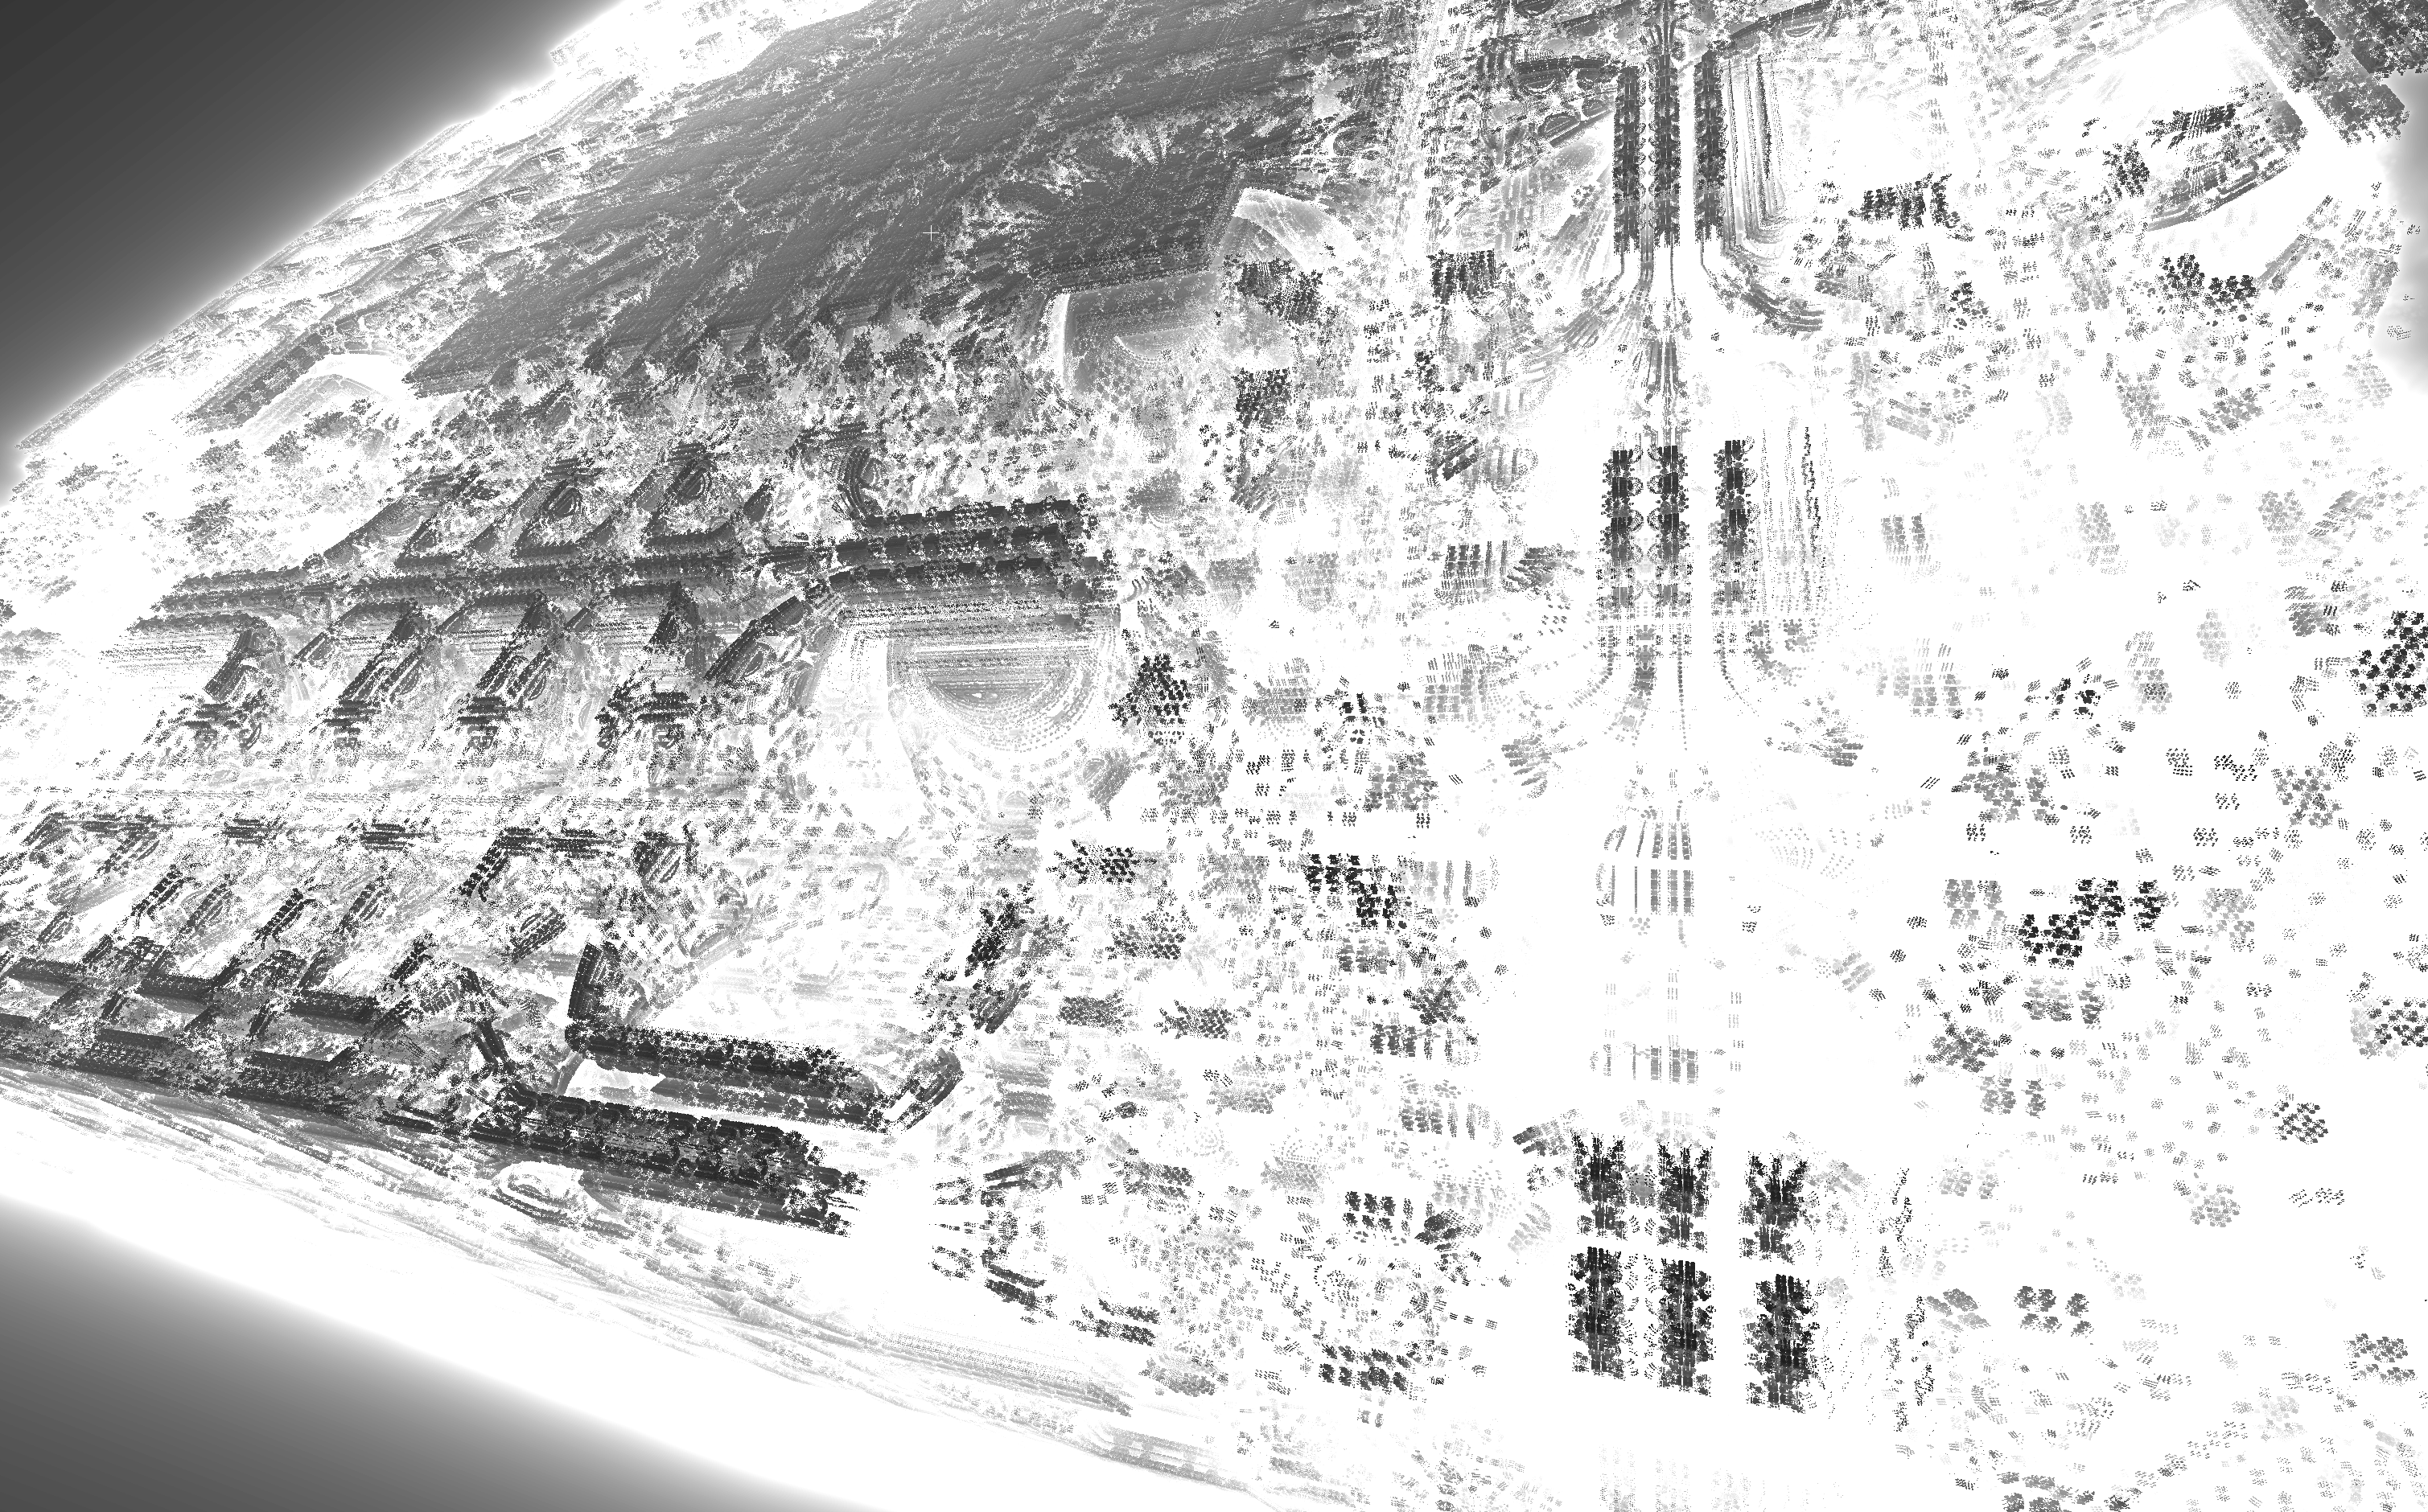
\includegraphics[width=\textwidth]{imgs/mandelbox_glsl_side.png}
        \label{fig:your_label}
    \end{minipage}
\end{center}

% ---------------------------------------------------------------
\subsection{Box Fold}
% ---------------------------------------------------------------

Each component of $\mathbf{v}$ is box-folded: if $|v_i| > 1$, it is reflected about
$\pm 1$:
%
\[
    \operatorname{BoxFold}(v_i) =
    \begin{cases}
        \phantom{-}2 - v_i  & \text{if } v_i > 1,  \\
        -2 - v_i             & \text{if } v_i < -1, \\
        \phantom{-}v_i       & \text{otherwise.}
    \end{cases}
\]

The fold limit acts as a container: reflections about $\pm1$ layer copies of space on top of each other, producing the self-similar nested structure characteristic of a fractal boundary.

% ---------------------------------------------------------------
\subsection{Sphere Fold}
% ---------------------------------------------------------------

The sphere fold prevents box-folded points near the origin from collapsing under scaling. Two concentric spheres ($m=0.5$, $f=1.0$) define three radial zones; points inside the inner sphere are repelled by inversion:
%
\[
    \mathbf{p}_{\text{out}} = \frac{f^{2}}{\|\mathbf{p}_{\text{in}}\|^{2}}\,\mathbf{p}_{\text{in}}.
\]
%
This smooths the sharp corners of the box fold into curved fractal boundaries.

\[
    \text{SphereFold}(\mathbf{v}) =
    \begin{cases}
        4\,\mathbf{v}                          & r^2 < m^2 \quad \text{(fixed scale; prevents underflow)} \\
        \mathbf{v}/r^2                         & m^2 \leq r^2 < f^2 \quad \text{(full inversion, } 1 < g < 4\text{)} \\
        \mathbf{v}                             & r^2 \geq f^2 \quad \text{(unchanged)}
    \end{cases}
\]

% ---------------------------------------------------------------
\subsection{Scaling, Translation and Derivatives}
% ---------------------------------------------------------------

Following the box and sphere folds, this step zooms towards the origin and shifts by
$\mathbf{c}$:
%
\[
    \mathbf{v}_{n+1} = s\,\mathbf{v}_{\text{folded}} + \mathbf{c},
\]
%
where $s$ is the scale factor and $\mathbf{c}$ is the original point. Zooming into folded
space over iterations produces finer scale and detail. A negative scale applies a uniform
scaling and reflection simultaneously. This alternating reflection, combined with the
subsequent box fold, creates the characteristic inside-out cubic symmetry of the Mandelbox.

To maintain the distance field estimate, the derivative magnitude $dr$ is updated in
parallel using the spherical scaling multiplier $g$:
%
\[
    dr_{n+1} = |s|\cdot g\cdot dr_{n} + 1.
\]

% ---------------------------------------------------------------



\subsection{Results}

\begin{table}[htbp]
\centering
\small
\caption{Timing results --- scaffold vs.\ Mandelbox}
\label{tab:timing}
{\renewcommand{\arraystretch}{1.3}
\begin{tabular}{lcc}
\toprule
\textbf{Metric} & \textbf{Scaffold} & \textbf{Mandelbox} \\
\midrule
\code{SDF\_LAT}   & 107 cycles & 230 cycles \\
Clock             & 125\,MHz   & 100\,MHz   \\
WNS               & $+3.170$\,ns & $+3.216$\,ns \\
Failing endpoints & 0 & 0 \\
\bottomrule
\end{tabular}}
\end{table}

\FloatBarrier

The Mandelbox required reducing the clock to 100\,MHz; the iterated fold logic
exceeds the 8\,ns timing budget at 125\,MHz due to the depth of the conditional
fold chain.

  % ---------------------------------------------------------------                                                         
  \subsection{SystemVerilog Implementation}                                                                                 
  % ---------------------------------------------------------------                                                         
                                                                                                                            
  The Mandelbox SDF is implemented as a fully pipelined \texttt{scene\_sdf}
  module in SystemVerilog. All arithmetic uses the project-wide FP27 custom
  float library (\texttt{fp\_add}, \texttt{fp\_mul}, \texttt{fp\_sub},
  \texttt{fp\_isqrt}). There are no loops or iterative feedback paths,
  each of the 4 Mandelbox iterations is unrolled as a distinct pipeline
  stage chained sequentially.

  \subsubsection*{Per-Iteration Pipeline (49 cycles)}

  Each iteration applies box fold $\to$ $r^2$ $\to$ sphere fold $\to$
  scale\,+\,offset in four stages:

  \begin{table}[h!]
  \centering
  \caption{Pipeline stages per Mandelbox iteration}
  \begin{tabular}{clr}
  \hline
  \textbf{Stage} & \textbf{Operation} & \textbf{Cycles} \\
  \hline
  A & Box fold: \texttt{fp\_clamp1} (comb.) $+$ \texttt{fp\_sub} $\times 3$ & 4 \\
  B & $r^2 = x^2+y^2+z^2$: \texttt{fp\_mul}$\times 3$ $+$ \texttt{fp\_add}$\times 2$ & 12 \\
  C & Sphere fold: \texttt{fp\_isqrt} $+$ \texttt{fp\_mul}$^2$ $+$ mux reg & 25 \\
  D & Scale $+$ offset: \texttt{fp\_mul}$\times 3$ $+$ \texttt{fp\_add}$\times 3$ & 8 \\
  \hline
  \textbf{Total} & & \textbf{49} \\
  \hline
  \end{tabular}
  \end{table}

  \noindent The box fold is combinatorial; \texttt{fp\_clamp1} examines
  bit\,[25:0] against the FP27 encoding of 1.0 and \texttt{fp\_times2}
  increments the exponent field by 1, both in zero cycles:

  \begin{verbatim}
  function automatic [26:0] fp_clamp1(input [26:0] a);
      fp_clamp1 = (a[25:0] > {8'h7F,18'h0}) ? {a[26],8'h7F,18'h0} : a;
  endfunction

  function automatic [26:0] fp_times2(input [26:0] a);
      fp_times2 = (a[25:18]==8'd0) ? 27'h0 : {a[26],a[25:18]+8'd1,a[17:0]};
  endfunction
  \end{verbatim}

  \noindent The sphere fold computes $1/r^2$ via \texttt{fp\_isqrt} followed
  by a squaring multiply, then selects between three zones at a registered mux:

  \begin{verbatim}
  //zone flags registered at cycle N+1 after r^2 arrives
  always @(posedge clk) begin
      inner_r <= (r2[25:0] < FP_0P25[25:0]); //r^2 < 0.25
      outer_r <= (r2[25:0] < FP_ONE[25:0]);  //r^2 < 1.0
  end

  //mux at cycle N+25
  always @(posedge clk) begin
      xs <= inner_r ? fp_times2(fp_times2(xf)) :  //x4
            outer_r ? x_outer                    :  //x/r^2
                      xf;                           //unchanged
  end
  \end{verbatim}

  \subsubsection*{Unrolled Iteration Timing}

  The four iterations are chained; companion signals use \texttt{state\_pipe}
  shift registers to maintain cycle-accurate alignment:

  \begin{table}[h!]
  \centering
  \caption{Cycle boundaries of each unrolled iteration}
  \begin{tabular}{lrr}
  \hline
  \textbf{Iteration} & \textbf{Input cycle} & \textbf{Output cycle} \\
  \hline
  Pre-register     & 0   & 1   \\
  Iteration 1      & 1   & 50  \\
  Iteration 2      & 50  & 99  \\
  Iteration 3      & 99  & 148 \\
  Iteration 4      & 148 & 197 \\
  \texttt{fp\_length} & 197 & 229 \\
  Scale $\times 0.2$  & 229 & 233 \\
  Output register     & 233 & 234 \\
  \hline
  \textbf{SDF\_LAT} & \multicolumn{2}{r}{\textbf{234 cycles}} \\
  \hline
  \end{tabular}
  \end{table}

  \noindent The distance estimate is $\|z_4\| \times 0.2$, a conservative
  lower bound on $\|z_4\|\,/\,|s|^4 = \|z_4\|\,/\,5.0625$. This prevents
  the ray marcher from overstepping near the fractal boundary. The constant
  0.2 is encoded exactly in FP27 as
  \texttt{\{1'b0,\,8'h7C,\,18'h26666\}}.

  The module uses 48 \texttt{fp\_mul} instances across 4 iterations (12 per
  iteration), consuming 48 DSP48E1 blocks on the Zynq-7020 which has 220
  available within budget.

% ===============================================================
\section{HDMI Output}
% ===============================================================

We implemented the initial HDMI output subsystem using an on-chip BRAM
framebuffer, establishing the display pipeline and providing the project's first
end-to-end proof that the PL could produce a visible image on the monitor.

\code{framebuffer\_bram.sv} implements a dual-port BRAM: one port accepts write
operations from the render pipeline; the second drives continuous scan-out for
\code{hdmi\_timing.sv}. \code{iter\_to\_rgb.sv} maps completed ray iteration
counts to 24-bit RGB using a pre-computed look-up table (\code{fog\_lut.mem}),
applying a fog gradient that serves as a perceptual depth cue. As discussed earlier, the BRAM framebuffer was replaced by AXI VDMA in the
final design, as the $1024 \times 600 \times 32$-bit frame (24.6\,Mbit) far
exceeds the available BRAM (4.9\,Mbit). The older colour mapping and timing
modules were retained.


% ===============================================================
\section{Audio FFT Pipeline}
% ===============================================================

\subsection{Design Evolution}
Initial design used Xilinx FFT IP with AXI-DMA to compute frequency
bands in hardware on the PL. As discussed in Section~1.4, this was replaced by
a software FFT on the host PC. The hardware FFT IP block design
(\code{audio\_fft.bd}) and \code{fft\_bridge.v} remain in the repository as
reference.

\subsection{Software FFT Pipeline}
A 1024-point FFT is computed per audio block at 44.1\,kHz using
\code{numpy.fft.rfft} on the host PC, with bin spacing
$\Delta f = 44100/1024 \approx 43.1$\,Hz.

\begin{table}[htbp]
\centering
\small
\caption{FFT frequency band definitions}
\label{tab:fft_bands}
{\renewcommand{\arraystretch}{1.3}
\begin{tabular}{lll}
\toprule
\textbf{Band} & \textbf{Frequency Range} & \textbf{FFT Bins} \\
\midrule
Bass   & ${\sim}43$--$215$\,Hz   & 1--5    \\
Mid    & ${\sim}215$--$2024$\,Hz & 5--47   \\
Treble & ${\sim}2024$--$8061$\,Hz & 47--187 \\
\bottomrule
\end{tabular}}
\end{table}

\FloatBarrier

Exponential smoothing/EMA lerp ($\alpha = 0.3$) is applied to each band. Overall RMS
amplitude, spectral centroid, zero-crossing rate, and a beat detection flag
(energy $> 1.5\times$ the 20-frame rolling mean) are also computed. All eleven
features are packed as IEEE\,754 floats and streamed to the PYNQ over TCP.

\subsection{Mapping to SDF Parameters}

\begin{table}[htbp]
\centering
\small
\caption{Audio feature to SDF parameter mapping}
\label{tab:audio_mapping}
{\renewcommand{\arraystretch}{1.3}
\begin{tabular}{lll}
\toprule
\textbf{Feature} & \textbf{SDF register} & \textbf{Hardware effect} \\
\midrule
Bass energy       & \code{sdf\_params[0]} (\code{cell\_sz}) & Space tiling period \\
Mid energy        & \code{sdf\_params[1]} (\code{b\_fp})    & Geometry arm half-length \\
Treble energy     & \code{sdf\_params[2]} (\code{e\_fp})    & Strut edge thickness \\
RMS               & Camera orbit radius                       & Camera pull-in/out \\
Spectral centroid & Camera $y$ offset                        & Camera height \\
\bottomrule
\end{tabular}}
\end{table}

\FloatBarrier

% =============================================================
  \section{IMU}
  % =============================================================                                                           
   
  The MPU-6050 IMU is polled at 100\,Hz via a custom MMIO driver accessing                                                  
  the AXI IIC core at \texttt{0x41600000}. Standard \texttt{smbus} tooling
  cannot be used as the I$^2$C bus is routed through the PL fabric rather
  than the PS I$^2$C controller.

  Orientation is tracked with a complementary filter:
  \[
    R \leftarrow \alpha\,(R + \omega\,\Delta t) + (1-\alpha)\,R_{\text{accel}},
    \qquad \alpha = 0.98
  \]
  The gyroscope term dominates (98\%), with 2\% accelerometer blending to
  correct long-term drift. Gram--Schmidt re-orthogonalisation is applied
  after every update to prevent floating-point rounding from skewing the
  lookat matrix over time:
  \[                                                                                                                        
    \hat{r}_0 = \frac{r_0}{\|r_0\|}, \qquad
    \hat{r}_1 = \frac{r_1 - (r_1 \cdot \hat{r}_0)\,\hat{r}_0}                                                               
                     {\|r_1 - (r_1 \cdot \hat{r}_0)\,\hat{r}_0\|}, \qquad
    \hat{r}_2 = \hat{r}_0 \times \hat{r}_1
  \]

  Movement impulses are projected onto the current rotation matrix columns
  rather than world axes:

  \begin{center}
  \begin{tabular}{ll}
  \hline
  \textbf{Key} & \textbf{Direction} \\
  \hline
  W / S        & $\pm R[:,2]$ (forward) \\
  A / D        & $\pm R[:,0]$ (right)   \\
  Space / C    & $\pm R[:,1]$ (up)      \\
  \hline
  \end{tabular}
  \end{center}

  This fixed a controls-inversion bug where translating in absolute world
  coordinates caused movement to reverse direction once the camera passed
  the scene origin.

% ===============================================================
\section{Neural SDF Training Pipeline}
% ===============================================================

\subsection{Motivation and Background}

An SDF returns the shortest distance from any 3D point to the nearest surface
boundary. Though closed-form analytic SDFs exist for simple shapes, no strict
formula is derivable for complex geometry such as fractals or organic meshes.
A Neural SDF approximates the SDF by training on sampled point-distance pairs;
the trained network can then be queried at any 3D coordinate.

\subsection{Network Architecture and Quantisation}

The chosen architecture is a $3\to32\to32\to32\to1$ MLP with ReLU activations.
ReLU reduces to an elementary comparator and multiplexer in hardware, eliminates
the vanishing gradient problem, and maintains unit gradient through all hidden
layers. No activation is applied to the output neuron, since signed distances
must be capable of representing negative values for interior points.

While 32 neurons per layer proved sufficient for simple geometry (sphere, torus),
complex fractal parameters required upgrading to 64 neurons. Weights are
quantised from \texttt{float32} to Q4.12 fixed-point: representable range
$\pm 8.0$, resolution $2^{-12} \approx 0.000244$.

\subsection{Training Pipeline}

Training data is generated by sampling 500,000 random points from $[-2, 2]^3$
and computing ground-truth SDF values analytically. The dataset is split 80/20
and trained with Adam optimiser and MSE loss in batches of 4096.

\subsection{Results}

\begin{table}[htbp]
\centering
\small
\caption{Neural SDF training results}
\label{tab:neural_results}
{\renewcommand{\arraystretch}{1.3}
\begin{tabular}{llc}
\toprule
\textbf{Shape} & \textbf{Architecture} & \textbf{Test Loss} \\
\midrule
Sphere    & $3\to32\to32\to32\to1$ & 0.000031 \\
Torus     & $3\to32\to32\to32\to1$ & 0.000053 \\
\bottomrule
\end{tabular}}
\end{table}

\FloatBarrier

\subsection{Weight Export}

Following training, weights are exported in Q4.12 hex format:
\begin{lstlisting}[language=Python]
format(int(round(w * 4096)) & 0xFFFF, '04x')
\end{lstlisting}
The 32-neuron network produces 260 files (\code{w\_\{layer\}\_\{neuron\}.hex},
\code{b\_\{layer\}\_\{neuron\}.hex}), directly parseable by Verilog
\code{\$readmemb}.


% ===============================================================
\section{Neural SDF Hardware Architecture}
\label{sec:neural_hw}
% ===============================================================

\subsection{Inference Engine Design}

Following the software training pipeline, it was proposed that the hardware inference
engine would consume the exported Q4.12 weights at synthesis time and
perform real-time MLP evaluation in the PL. The design comprises three modules:
\code{neuron\_layer.sv}, \code{sdf\_nn.sv}, and a trilinear interpolation cache
\code{trilinear\_interp.sv}.
Why Q4.12? 
Q4.12 was chosen as the weight format for three reasons.
First, each weight occupies a single 16-bit word, keeping BRAM usage half
that of \texttt{float32} weights.
Second, a 16-bit signed multiply fits natively into a single \texttt{DSP48E1}
18$\times$18 multiplier, the same primitive used throughout the FP27
library, whereas \texttt{float32} would require four DSP slices per weight
multiply.
Third, the four integer bits give a representable range of $[-8,\,8)$,
sufficient for the normalised weight magnitudes produced by the PyTorch
training pipeline, and the twelve fractional bits give a resolution of
$2^{-12}\approx2.4\times10^{-4}$, which was found adequate to keep inference
error below $0.5\%$ on the training geometry.

\code{neuron\_layer.sv} implements one fully connected layer. Weights for each
neuron are baked into BRAM at synthesis via \code{\$readmemb}, which reads the
hex files exported by the training script. The dot product is computed across
all input neurons in parallel using an array of Q4.12 fixed-point multipliers,
then accumulated with a final bias addition. A ReLU gate (implemented as a sign
bit comparator and output mux) is applied when the \code{USE\_RELU} parameter
is set; the output layer instantiates the module with \code{USE\_RELU = 0} to
allow signed distance outputs. For the 32-neuron hidden layers, 32 multipliers
run in parallel, accumulating into a 32-bit sum in $\log_2 32 = 5$ adder stages
(binary adder tree), plus one pipeline register per stage, giving a layer latency
of approximately 10 clock cycles.

\code{sdf\_nn.sv} chains three \code{neuron\_layer} instances (two hidden,
one output) and presents the same uniform interface as the analytic SDF modules
(inputs \code{px}, \code{py}, \code{pz}, output \code{sdf\_out}) allowing
it to be substituted into \code{march\_core} without any pipeline changes beyond
updating the \code{SDF\_LAT} parameter.

Crucially, the inference latency is fully deterministic. Every Q4.12
multiply-accumulate operation completes in a fixed number of clock cycles:
the parallel weight multiplications across all input neurons fire simultaneously,
their products are summed through a binary adder tree of fixed depth
$\lceil\log_2 N\rceil$ for $N$ inputs, a bias is added, and ReLU is applied
, all in a fixed pipeline with no data-dependent branching.
Chaining three such layers gives a total MLP latency that is a compile-time
constant, exactly as \code{SDF\_LAT} is for the analytic scenes.
The march pipeline makes no distinction between analytic and neural SDFs:
it simply waits \code{SDF\_LAT} cycles after presenting coordinates before
sampling the result, regardless of what is inside the SDF module.


\subsection{Trilinear Interpolation Cache}

The 3D coordinate space is partitioned into a coarse voxel grid (see as 32 x 32 x 32 cubes). At synthesis
the SDF is precomputed at each grid vertex and stored in BRAM (\code{trilinear\_interp.sv})- that's the baking approach.
At runtime, the eight vertices surrounding a query point are read from BRAM and
their SDF values are linearly interpolated along each axis in sequence, replacing
the full MLP forward pass with eight BRAM reads and 7 multiply-accumulate
operations. This is significantly cheaper than the full inference chain and was
intended as a performance/accuracy tradeoff for low-complexity scenes. Indeed, full SDF neural inference (initially opted for) would require a neural inference pass per march, which blows computational throughput.

\begin{figure}[h!]
\centering
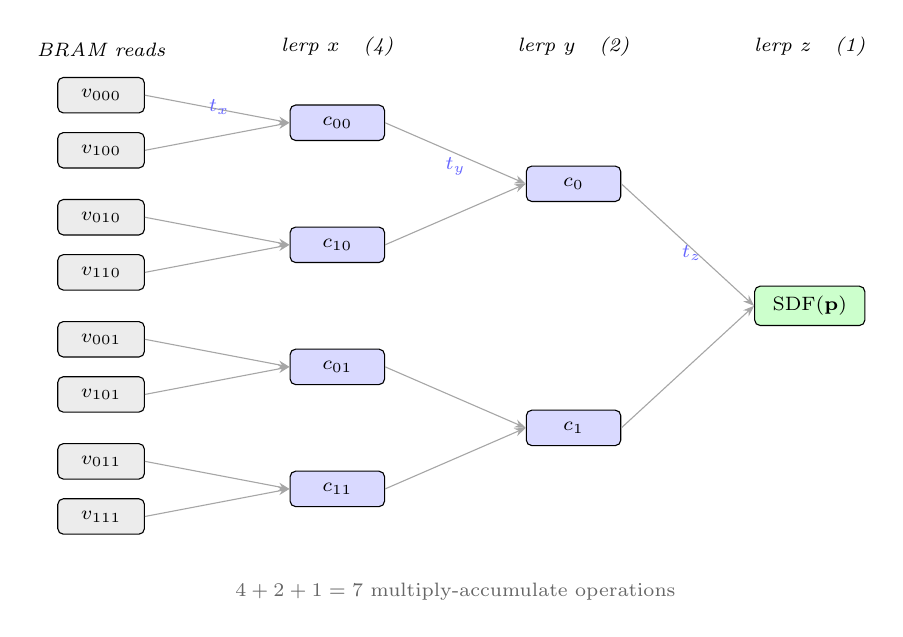
\begin{tikzpicture}[
  node distance=0.7cm,
  bram/.style={draw, fill=gray!15, rounded corners=2pt,
               minimum width=1.1cm, minimum height=0.45cm, font=\scriptsize},
  lerp/.style={draw, fill=blue!15, rounded corners=2pt,
               minimum width=1.2cm, minimum height=0.45cm, font=\scriptsize},
  res/.style={draw, fill=green!20, rounded corners=2pt,
              minimum width=1.4cm, minimum height=0.5cm, font=\scriptsize\bfseries},
  arr/.style={-{Stealth[length=4pt]}, gray!70},
  lbl/.style={font=\scriptsize\itshape},
]

%% ---- Column 0: BRAM reads (8 vertices) ----
\node[bram] (v000) at (0, 0.00) {$v_{000}$};
\node[bram] (v100) at (0,-0.70) {$v_{100}$};
\node[bram] (v010) at (0,-1.55) {$v_{010}$};
\node[bram] (v110) at (0,-2.25) {$v_{110}$};
\node[bram] (v001) at (0,-3.10) {$v_{001}$};
\node[bram] (v101) at (0,-3.80) {$v_{101}$};
\node[bram] (v011) at (0,-4.65) {$v_{011}$};
\node[bram] (v111) at (0,-5.35) {$v_{111}$};

\node[lbl, above=2pt] at (0, 0.3) {BRAM reads};

%% ---- Column 1: lerp along x (4 ops) ----
\node[lerp] (c00) at (3.0,-0.35) {$c_{00}$};
\node[lerp] (c10) at (3.0,-1.90) {$c_{10}$};
\node[lerp] (c01) at (3.0,-3.45) {$c_{01}$};
\node[lerp] (c11) at (3.0,-5.00) {$c_{11}$};

\node[lbl, above=2pt] at (3.0, 0.3) {lerp $x$\quad(4)};

\draw[arr] (v000.east) -- (c00.west);
\draw[arr] (v100.east) -- (c00.west);
\draw[arr] (v010.east) -- (c10.west);
\draw[arr] (v110.east) -- (c10.west);
\draw[arr] (v001.east) -- (c01.west);
\draw[arr] (v101.east) -- (c01.west);
\draw[arr] (v011.east) -- (c11.west);
\draw[arr] (v111.east) -- (c11.west);

%% ---- Column 2: lerp along y (2 ops) ----
\node[lerp] (cy0) at (6.0,-1.125) {$c_{0}$};
\node[lerp] (cy1) at (6.0,-4.225) {$c_{1}$};

\node[lbl, above=2pt] at (6.0, 0.3) {lerp $y$\quad(2)};

\draw[arr] (c00.east) -- (cy0.west);
\draw[arr] (c10.east) -- (cy0.west);
\draw[arr] (c01.east) -- (cy1.west);
\draw[arr] (c11.east) -- (cy1.west);

%% ---- Column 3: lerp along z (1 op) ----
\node[res] (result) at (9.0,-2.675) {$\mathrm{SDF}(\mathbf{p})$};

\node[lbl, above=2pt] at (9.0, 0.3) {lerp $z$\quad(1)};

\draw[arr] (cy0.east) -- (result.west);
\draw[arr] (cy1.east) -- (result.west);

%% ---- axis labels on edges ----
\node[lbl, color=blue!60] at (1.5,-0.15) {$t_x$};
\node[lbl, color=blue!60] at (4.5,-0.9) {$t_y$};
\node[lbl, color=blue!60] at (7.5,-2.0) {$t_z$};

%% ---- total op count ----
\node[font=\scriptsize, align=center, text=black!60]
  at (4.5,-6.3) {$4+2+1 = 7$ multiply-accumulate operations};

\end{tikzpicture}
\caption{Trilinear interpolation reduces eight BRAM-stored vertex SDF values
to a single query result in seven multiply-accumulate operations.
Interpolation weights $t_x,\,t_y,\,t_z \in [0,1]$ are the fractional
offsets of the query point within its voxel cell.}
\label{fig:trilinear}
\end{figure}

\begin{figure}[h!]
    \centering
    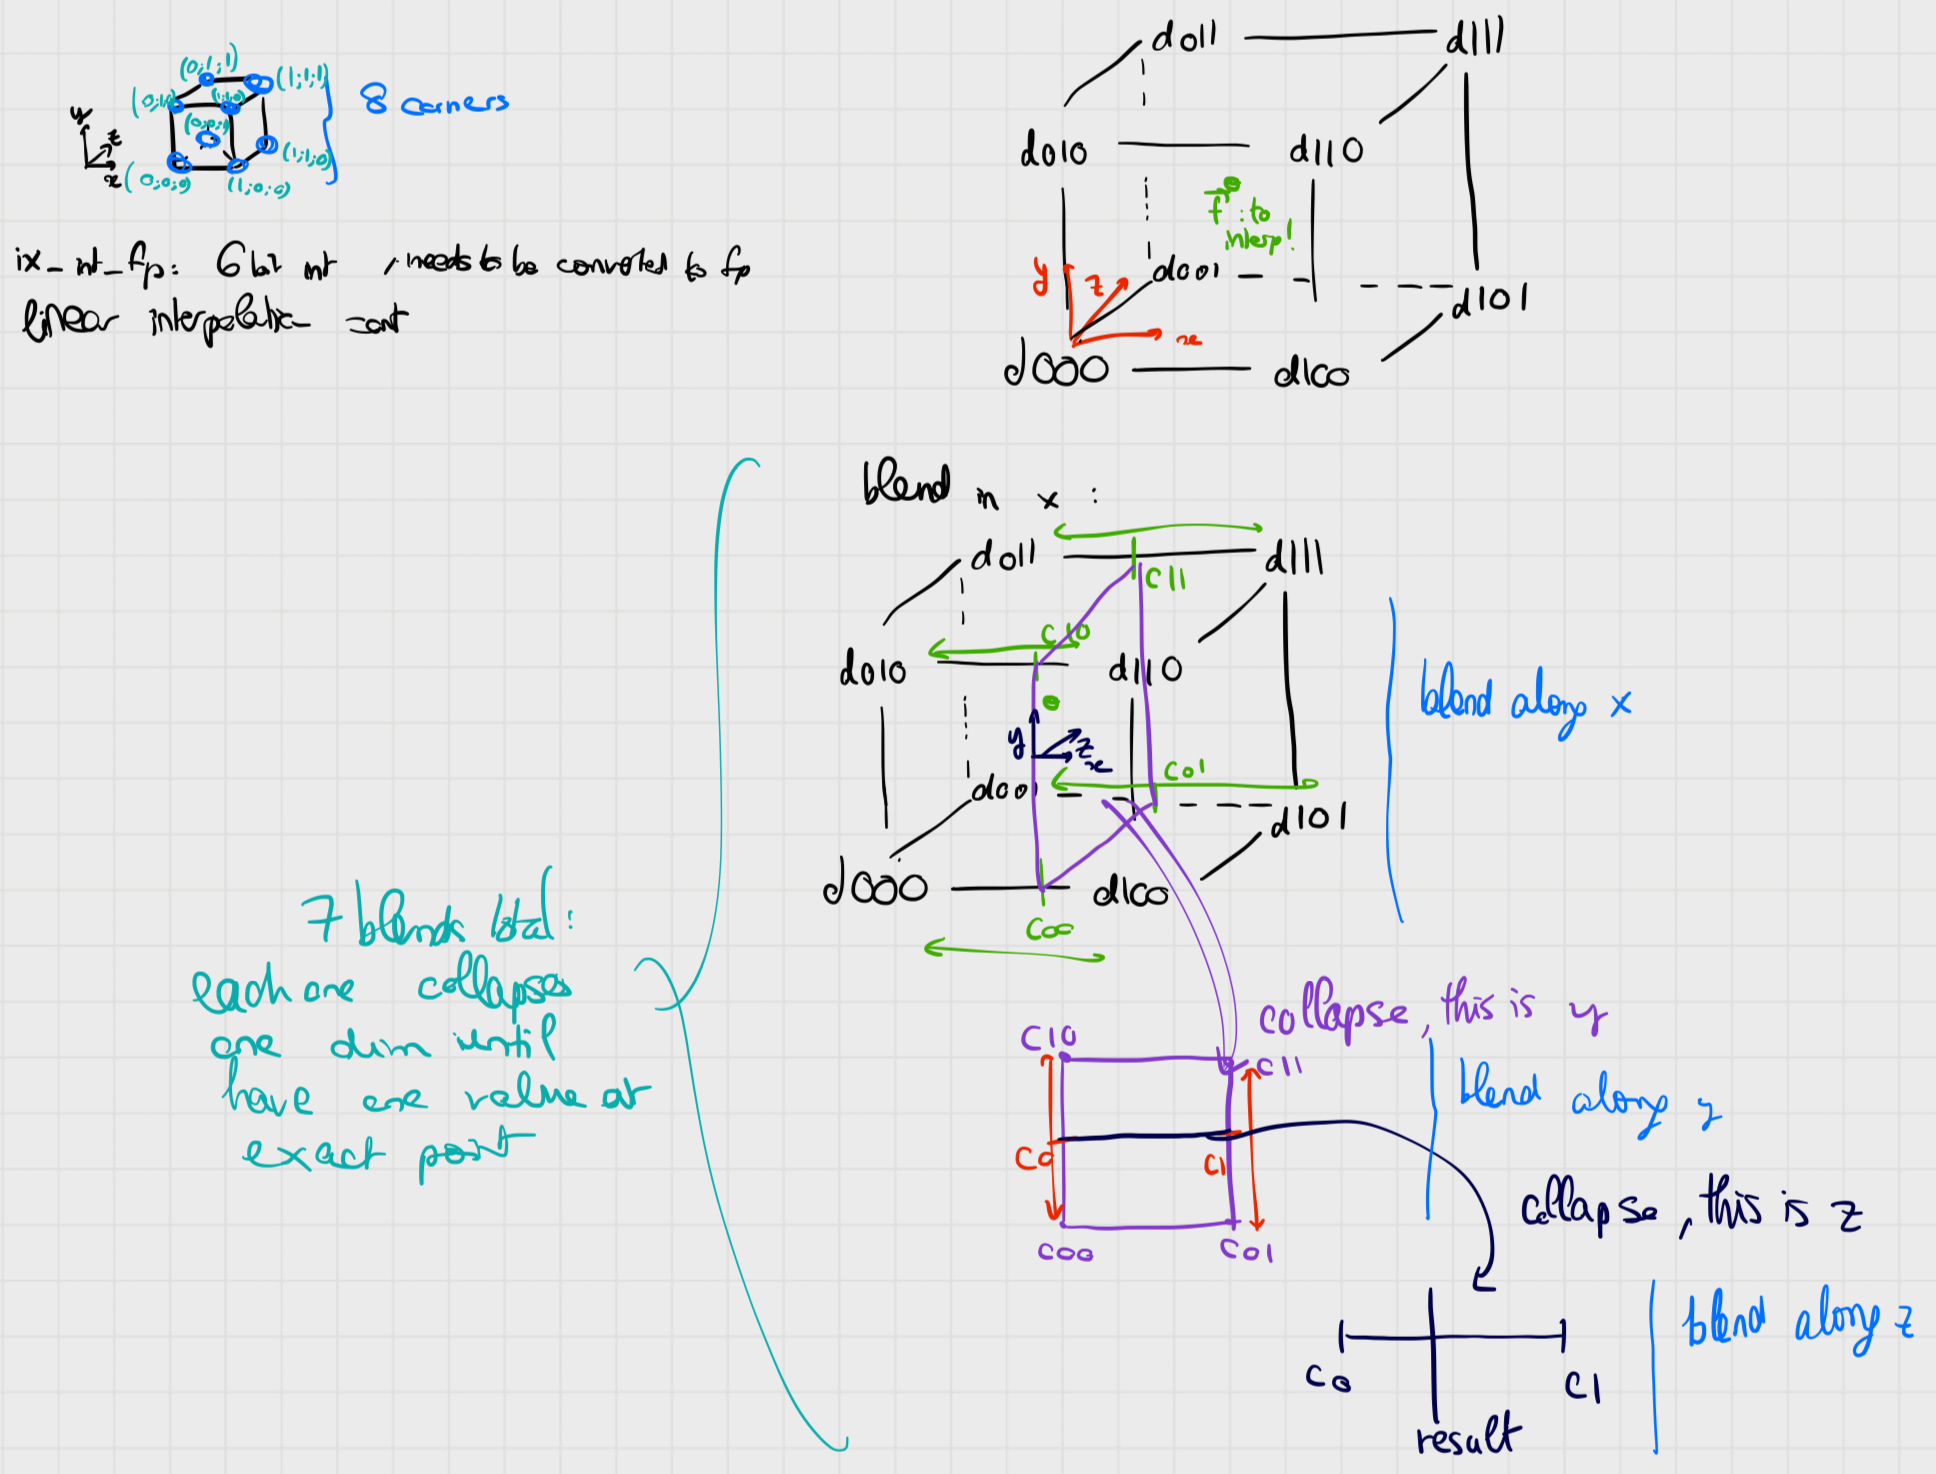
\includegraphics[width=0.8\textwidth]{imgs/lerp_visualized.png}
    \caption{A visual intuition as to how lerping is done in 3D}
    \label{fig:your_label}
\end{figure}

\subsection{Integration Status}

The training pipeline, weight export, and all hardware modules
(\code{neuron\_layer.sv}, \code{sdf\_nn.sv}, \code{trilinear\_interp.sv})
were implemented and synthesise without errors. The integration with
\code{march\_core} was not completed within the project timeline. The march
pipeline assumes a fixed-latency interface (one SDF result every clock cycle,
no backpressure). Since the MLP forward pass is fully pipelined with no
data-dependent branching, its latency is also a compile-time constant -
the fix is simply to count the pipeline stages across the three chained
\code{neuron\_layer} instances and set \code{SDF\_LAT} accordingly.
The integration was not completed within the project timeline and remains
as future work, but no architectural changes to \code{march\_core} are
required. Simply, it was feared that the DSP count on the PYNQ Z1 board could be easily exceeded when combining MLP + march core logic, as the single core version already consumed +30,000 LUTs and 140 DSPs. Pipelined use of DSPs would have to be considered, but we prefered to focus on the interactivity of our system through enhanced sound reactivity and smoother IMU control.



% ===============================================================
\section{Integrated Block Design and VDMA Pipeline}
\label{sec:vdma}
% ===============================================================

\subsection{Vivado Block Design}

The Vivado block design (\code{control\_bd.tcl}) connects all hardware subsystems.
The PS7 (ARM Cortex-A9) is the sole AXI-Lite master; it writes to the camera
register file and to the two AXI GPIO instances. On the high-performance path,
the AXI VDMA IP and the AXI framebuffer writer act as AXI4 masters, accessing
DDR3 through an AXI Interconnect that arbitrates between them and routes to the
PS7 HP slave port.

Key IP blocks:
\begin{itemize}
    \item \textbf{AXI VDMA}: reads completed frames from DDR3 and streams
    pixels to the RGB-to-DVI serialiser in park mode, looping on a fixed
    framebuffer.
    \item \textbf{rgb2dvi\_0}: converts 24-bit RGB pixel stream to TMDS
    differential pairs at 74.25\,MHz pixel clock.
    \item \textbf{clk\_wiz\_0}: generates 125\,MHz system clock and
    74.25\,MHz pixel clock from FCLK0 (50\,MHz from the PYNQ API).
    \item \textbf{AXI GPIO (0x41200000)}: two-channel GPIO for the
    frame-ready handshake: PL writes \code{frame\_ready\_valid} and
    \code{frame\_ready\_bank} on channel 1; PS writes \code{frame\_ack} on
    channel 2.
    \item \textbf{AXI GPIO (0x41210000)}: three push-button inputs read
    by the PS via MMIO for the scene selector UI.
\end{itemize}

\subsection{VDMA Double-Buffer Handshake}

The PL renders into one of two DDR3 framebuffers while the VDMA displays the
other. Frame synchronisation uses a two-signal AXI GPIO handshake implemented
in \code{ctrl.py}:

\begin{enumerate}
    \item PL finishes a complete frame, sets \code{frame\_ready\_valid = 1} and
    \code{frame\_ready\_bank = render\_bank}.
    \item PS polls the GPIO in \code{service\_frame\_ready()} and, on seeing
    \code{valid = 1}, calls \code{set\_display\_bank(vdma, ready\_bank)} to
    switch the VDMA park pointer to the completed buffer.
    \item PS pulses \code{frame\_ack = 1} for 1\,ms, then clears it.
    \item PL detects the ack, clears \code{frame\_ready\_valid}, and begins
    rendering the next frame into the other buffer.
\end{enumerate}

This handshake ensures no tearing: the VDMA pointer is updated only after a
complete frame is ready, and the PL does not overwrite a buffer while it is
being displayed.


\subsection{Integration Status}

The training pipeline, weight export, and all hardware modules
(\code{neuron\_layer.sv}, \code{sdf\_nn.sv}, \code{trilinear\_interp.sv})
were implemented and synthesise without errors. The integration with
\code{march\_core} was not completed within the project timeline. The march
pipeline assumes a fixed-latency interface (one SDF result every clock cycle,
no backpressure). Since the MLP forward pass is fully pipelined with no
data-dependent branching, its latency is also a compile-time constant -
the fix is simply to count the pipeline stages across the three chained
\code{neuron\_layer} instances and set \code{SDF\_LAT} accordingly.
The integration was not completed within the project timeline and remains
as future work, but no architectural changes to \code{march\_core} are
required. Simply, it was feared that the DSP count on the PYNQ Z1 board could be easily exceeded when combining MLP + march core logic, as the single core version already consumed +30,000 LUTs and 140 DSPs. Pipelined use of DSPs would have to be considered, but we prefered to focus on the interactivity of our system through enhanced sound reactivity and smoother IMU control.


% Chapter 3 — System Integration
\doublespacing

\chapter{System Integration}
\label{ch3}

\begin{spacing}{1}
\minitoc
\end{spacing}
\thesisspacing

\section{Block Diagram explained}

\subsection{VDMA Block Diagram and System Integration}

This section explains the software reference renderer, camera-control path, stereoscopic output and integration of the hardware ray marcher into a complete HDMI pipeline. We first built the software renderer to give the group a working algorithmic reference. We then modified the initial BRAM framebuffer design into a double-buffered HDMI output path before implementing the full VDMA/DDR system: Vivado integration, a custom AXI DDR writer, Python control software, frame-swap handshaking and audio-reactive control registers.

The software reference renderer was built as a React application with CPU and GPU scaffold renderers, a shaded sphere renderer, a free-flight camera and a live performance HUD. The CPU renderer generates a camera ray for each pixel, evaluates the scaffold signed-distance field and writes the colour into a canvas \texttt{ImageData} buffer. It runs at the same $512 \times 300$ internal resolution as the FPGA, making the comparison meaningful. The GPU version evaluates the same scaffold shader in parallel using WebGL 2, confirming that the algorithm maps well to per-pixel parallelism. The shaded sphere scene, with normal estimation, lighting, soft shadows, ambient occlusion and fog, was used to validate the camera maths before reducing the hardware target to the simpler iteration-coloured scaffold.

We represented the camera using a 3D origin and a $3 \times 3$ orientation matrix rather than sending yaw and pitch directly into the FPGA. Yaw and pitch are convenient for user input, but converting them into rays requires trigonometric functions and vector normalisation, which are cheaper in Python than in RTL. The host therefore computes the camera basis, while the FPGA receives ready-to-use vectors for per-pixel ray generation.

The Pygame controller maintains yaw, pitch, position and movement speed. Yaw rotates the view around the vertical axis, while pitch controls the vertical component. The forward vector is:
\begin{equation}
\mathbf{f} =
\begin{bmatrix}
\sin(\text{yaw})\cos(\text{pitch}) \
\sin(\text{pitch}) \
-\cos(\text{yaw})\cos(\text{pitch})
\end{bmatrix}.
\end{equation}

Here, $\sin(\text{pitch})$ gives the vertical component and $\cos(\text{pitch})$ gives the remaining horizontal length. Yaw splits this horizontal component between $x$ and $z$ using $\sin(\text{yaw})$ and $-\cos(\text{yaw})$, giving a unit-length forward vector without an extra host-side normalisation step.

The right vector is:
\begin{equation}
\mathbf{r} =
\begin{bmatrix}
\cos(\text{yaw}) \
0 \
\sin(\text{yaw})
\end{bmatrix}.
\end{equation}

This is perpendicular to the horizontal projection of the forward vector and has no $y$ component, so strafing stays level even when the user looks up or down. The up vector is calculated from the cross product of the right and forward vectors, completing an orthogonal camera frame.

These three vectors form the camera matrix:
\begin{equation}
M =
\begin{bmatrix}
r_x & u_x & f_x \\
r_y & u_y & f_y \\
r_z & u_z & f_z
\end{bmatrix}.
\end{equation}

A camera-space ray is rotated into world space by:
\begin{equation}
\mathbf{d}_{world}=d_x\mathbf{r}+d_y\mathbf{u}+d_z\mathbf{f}.
\end{equation}

A centre pixel has almost no right or up offset, so its ray points mainly along the forward vector. A top-right pixel has positive right and up offsets, so its ray becomes a weighted mixture of the right, up and forward vectors. This keeps the FPGA calculation simple while still allowing arbitrary camera orientation.

In hardware, the Pygame controller sends twelve 32-bit floating-point values over TCP: nine camera-matrix entries and three origin coordinates. On the PYNQ, the Python service converts each IEEE-754 value into the RTL's 27-bit floating-point format and writes it into the AXI-Lite camera register file. The conversion keeps the sign bit and 8-bit exponent, but rounds the mantissa to 18 bits. This preserves useful dynamic range while reducing FPGA arithmetic width. The same AXI-Lite interface also carries DDR framebuffer addresses and scene-control parameters.

The ray-generation module converts each incoming pixel coordinate into a camera-space ray. The $x$ and $y$ coordinates give horizontal and vertical offsets from the centre of the eye image, while a fixed forward-depth constant controls the field of view. These offsets are converted to 27-bit floating point, squared, summed and passed through the inverse-square-root block to normalise the ray. The design then applies the camera matrix using nine floating-point multiplications and six additions, with pipeline delays keeping camera data, pixel ID and ray components aligned.

The same camera system was extended for stereoscopic output. The rendered $512 \times 300$ internal frame is split into two 256-pixel-wide eye images. For the right eye, the ray generator subtracts 256 from the $x$ coordinate so each half has its own local screen coordinate system. The march core forms the eye origins by offsetting the camera origin along the right vector:
\begin{equation}
\mathbf{origin}_{left} = \mathbf{origin} - \mathbf{r}\cdot\text{half\_IPD}
\end{equation}
and the right-eye origin is:
\begin{equation}
\mathbf{origin}_{right} = \mathbf{origin} + \mathbf{r}\cdot\text{half\_IPD}.
\end{equation}

Both eyes use the same orientation matrix, but their origins are laterally separated. This produces the horizontal parallax needed for stereoscopic 3D while reusing the same ray-marching pipeline for both halves of the image.

The first FPGA display path used BRAM as the framebuffer. We modified it into a double-buffered design because a single framebuffer was unsafe when the renderer and HDMI scan-out operated concurrently. One BRAM bank was written by the render pipeline while the other was read by scan-out. The two buffers were stored back-to-back, with the write address offset by 153,600 when the render bank was high. The displayed bank changed only on vertical sync, preventing mid-frame buffer switches.

The BRAM scan-out path mapped the $512 \times 300$ internal render to $1024 \times 600$ HDMI output by duplicating each pixel horizontally and vertically. This kept the workload at 153,600 rays per frame while filling the headset display. The BRAM version was useful for debugging, but it used 120 out of 140 Block RAM tiles, or 85.71%, making the framebuffer the dominant resource constraint.

\begin{figure}[htbp]
\centering
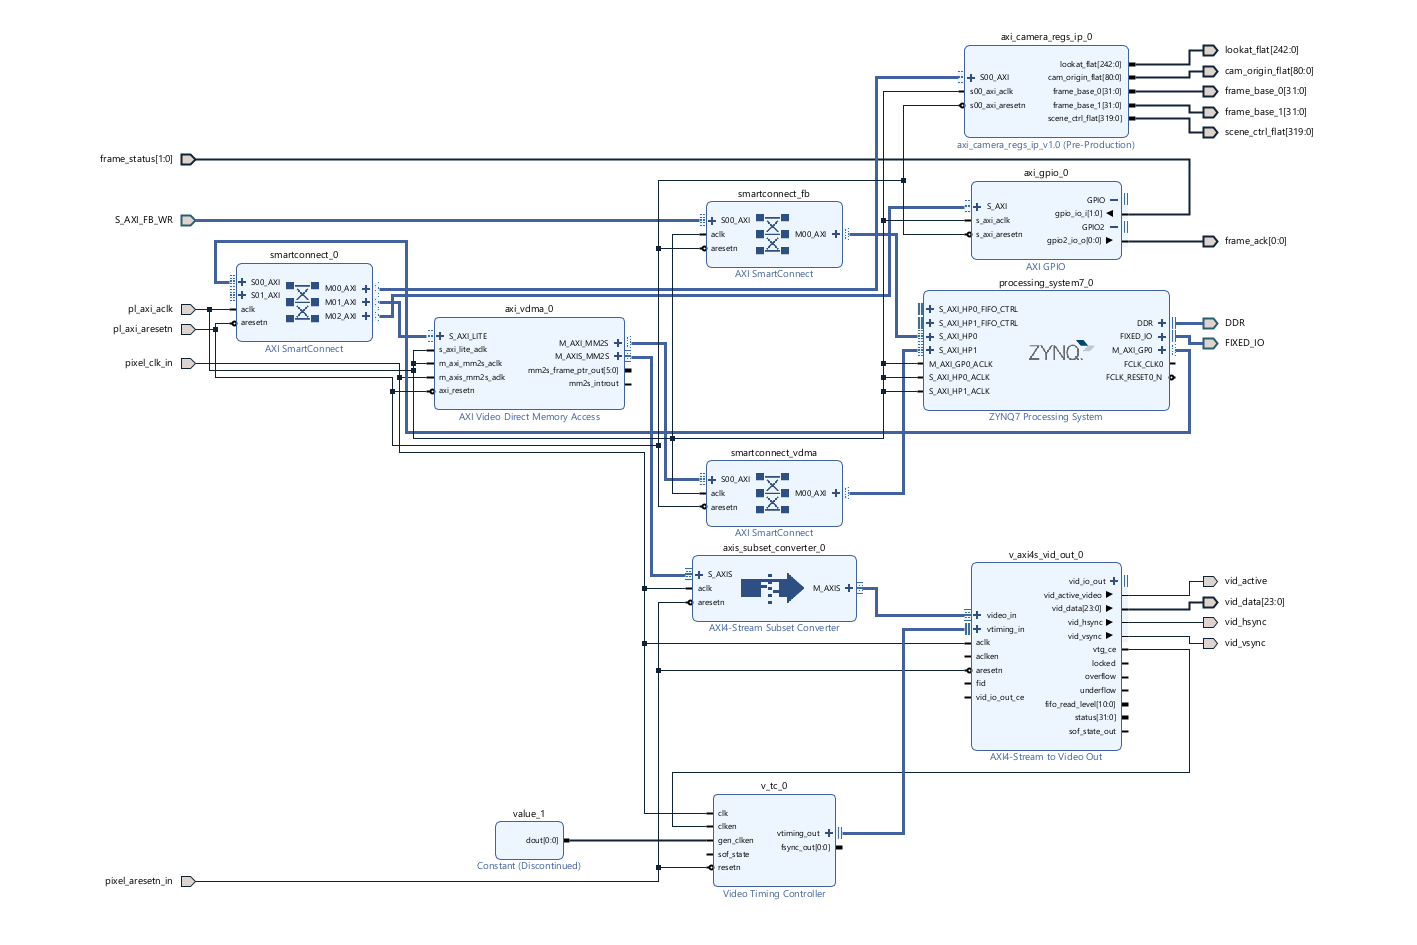
\includegraphics[width=0.95\linewidth]{imgs/vdma_block_diagram.png}
\caption{Vivado block diagram for the VDMA-based HDMI output architecture. The design separates low-bandwidth AXI-Lite control traffic from high-bandwidth frame-buffer traffic through DDR.}
\label{fig:vdma-block-diagram}
\end{figure}

The VDMA version replaced the BRAM framebuffer with two frame buffers in external DDR. Figure~\ref{fig:vdma-block-diagram} shows the final Vivado block design, built around the Zynq processing system, custom accelerator IP, AXI VDMA, AXI GPIO, video timing controller, AXI4-Stream-to-video-out, AXI-stream subset conversion, RGB-to-DVI and SmartConnect blocks. GP0 handles low-bandwidth AXI-Lite control, including the camera/scene registers at \texttt{0x43C00000}, VDMA control at \texttt{0x43000000} and GPIO at \texttt{0x41200000}. The high-bandwidth frame paths are separate: the custom writer reaches DDR through HP0, while the VDMA reads display frames through HP1. The CPU configures the system and swaps buffers, but never transfers pixels itself.

The VDMA is configured only in memory-to-stream mode because the FPGA writes rendered frames using its own AXI master. The PYNQ software allocates two non-cacheable $1024 \times 600$ \texttt{uint32} buffers in DDR and writes their physical addresses into both the VDMA start-address registers and accelerator framebuffer-base registers. The VDMA uses a 4096-byte horizontal size, 4096-byte stride and 600 lines, matching a $1024 \times 600$ frame with 32 bits per pixel. It runs in park mode so software can choose which buffer is displayed. The VDMA stream then passes through the video output path, where the 24 RGB bits are extracted before HDMI output.

The custom DDR writer receives completed ray results as a pixel ID and 8-bit iteration count. The palette converts this to 24-bit RGB, then the render bank, pixel ID and colour are packed into a 45-bit FIFO entry. The 4096-entry FIFO isolates the ray-marching pipeline from the AXI write interface: if DDR writes stall, completed pixels accumulate; if the FIFO approaches full, the top-level controller stalls new dispatch before data is lost.

The DDR writer also performs the $2 \times 2$ scaling from $512 \times 300$ render resolution to $1024 \times 600$ display resolution. Each internal result at $(x,y)$ becomes four output pixels. Rather than issuing four separate 32-bit writes, each horizontal pair is packed into one 64-bit AXI beat:
\begin{equation}
{\texttt{8'h00},\ \texttt{rgb},\ \texttt{8'h00},\ \texttt{rgb}}.
\end{equation}
Repeating this write one display row lower reduces each internal pixel to two 64-bit writes and uses the full HP0 data width.

The DDR frame is linear, with 1024 pixels per row and 4 bytes per pixel, so each output row occupies 4096 bytes. Each internal row expands into two output rows and each internal column into two 32-bit output pixels, so the top-row address is:
\begin{equation}
\mathrm{addr}_{top}=\mathrm{base}+(y \times 8192)+(x \times 8).
\end{equation}

This maps naturally to hardware shifts because $y \times 8192$ is a left shift by 13 and $x \times 8$ is a left shift by 3. The second row of the $2 \times 2$ block is written by adding 4096 bytes. The resulting layout is exactly what the VDMA expects: a normal $1024 \times 600$, 32-bit-per-pixel linear frame.

The writer uses AXI single-beat incrementing writes. \texttt{AWLEN} is zero, \texttt{AWSIZE} selects an 8-byte beat, \texttt{AWBURST} is incrementing and all byte strobes are enabled. Address and data channels are independent, so the writer keeps separate \texttt{w\_sent} and \texttt{w\_sent} flags, treats a beat as issued only once both handshakes complete and tracks B-channel responses with an outstanding-response counter. Up to eight outstanding writes are allowed, so the design does not assume a write has reached DDR simply because address and data were accepted by the interconnect.

Frame completion is controlled carefully. Dispatch stops after 153,600 internal rays have been issued, and completion is detected when 153,600 results return. However, the frame is not handed to the VDMA until the DDR writer is drained. This signal is asserted only when the result FIFO is empty, no active or prefetched entry remains, no beat is in progress, no delayed pixel is entering the writer and all outstanding write responses have returned. This ensures all pixels are safely visible in DDR before display.

Frame ownership is handled using AXI GPIO. Channel 1 carries frame-ready and completed-bank status bits from FPGA to Python, while Channel 2 carries the acknowledgement bit back. When a frame is drained, Python parks the VDMA on the completed bank and pulses acknowledgement for 1 ms. The FPGA then clears ready, toggles the render bank and starts the next frame. This prevents displaying an incomplete buffer or overwriting one still being displayed.

The Python control flow maps the camera register IP, VDMA and GPIO through MMIO, allocates two DDR frame buffers, writes default camera and scene values, writes framebuffer addresses to the accelerator and configures the VDMA. It also services the frame-ready handshake during camera socket timeouts, so display updates continue even when camera input is idle. Audio-reactive scene parameters are written through the same control path and latched at frame boundaries so each frame uses a consistent scene state.

The measured performance and resource results show the architectural trade-off. The CPU scaffold renderer averages approximately 1.2 FPS at $512 \times 300$, while the FPGA scaffold scene averages approximately 18.46 FPS after the VDMA/frame-ready handshake, corresponding to 54.22 ms per frame and a $15.4\times$ improvement by FPS. Moving from BRAM to DDR reduced framebuffer BRAM usage from 120 tiles to 3 tiles, at the cost of extra LUT, register and DSP usage from the AXI writer, DDR interconnect, VDMA path and control structure.

\subsection{Implementation utilisation and timing}

Table~\ref{tab:impl-utilisation} summarises post-implementation resource utilisation for the final VDMA design. The key result is low BRAM usage: only 3 out of 140 BRAM tiles, or 2.14%.

\begin{table}[htbp]
\centering
\caption{Post-implementation resource utilisation for the final VDMA design.}
\label{tab:impl_utilisation}
\begin{tabular}{|l|r|r|r|}
\hline
Resource & Used & Available & Utilisation \\
\hline
Slice LUTs & 22,366 & 53,200 & 42.04\% \\
Slice registers & 13,499 & 106,400 & 12.69\% \\
Slices & 6,844 & 13,300 & 51.46\% \\
BRAM tiles & 3 & 140 & 2.14\% \\
DSP48E1 & 62 & 220 & 28.18\% \\
Bonded IOB & 10 & 125 & 8.00\% \\
BUFGCTRL & 4 & 32 & 12.50\% \\
MMCM & 1 & 4 & 25.00\% \\
\hline
\end{tabular}
\end{table}

The post-route timing report showed that all specified constraints were met. The worst setup slack was 0.123 ns and the worst hold slack was 0.016 ns, with no failing setup or hold endpoints. The design was valid after implementation, although the small margins show that the final VDMA build was close to the timing limit.

\begin{table}[htbp]
\centering
\caption{Post-route timing summary for the final VDMA design.}
\label{tab:timing_summary}
\begin{tabular}{|l|r|}
\hline
Timing metric & Value \\
\hline
Setup WNS & 0.123 ns \\
Setup TNS & 0.000 ns \\
Setup failing endpoints & 0 \\
Hold WHS & 0.016 ns \\
Hold THS & 0.000 ns \\
Hold failing endpoints & 0 \\
Pulse-width worst slack & 1.740 ns \\
Routed nets with errors & 0 \\
\hline
\end{tabular}
\end{table}

The main implementation clock was \verb|clk_out1_clk_wiz_0| at 140.016 MHz. The design also used \verb|clk_out2_clk_wiz_0| at 51.339 MHz for the video path and \verb|clk_out3_clk_wiz_0| at 256.696 MHz with few loads. Four global clock buffers and one MMCM were used. The routed design contained 30,837 routable nets, all fully routed with no errors.

\section{UI and Bitstream Switching}

Crucial to our design, we wanted to be able to switch scenes through a UI. Given the high LUT usage, and that each signed distance function counts for at minimum 3,000 LUTs, it was unfeasible to have all SDFs on one bitstream. Bitstream switching had to be developped.

\subsection{Scene Selector}

The graphical scene selector is rendered directly into a VDMA-backed DDR3
framebuffer and displayed over the same HDMI output as the ray marcher,
eliminating the need for a separate display or serial terminal. The UI is
implemented in Python on the PYNQ Linux stack (\texttt{selector.py}) and
runs on a dedicated \texttt{ui.bit} bitstream whose sole purpose is to drive
the VDMA and accept button input; no ray marching hardware is loaded
during menu navigation.

A pre-rendered PNG (\texttt{base\_ui.png}) is loaded once at startup,
converted to a $1024\times600$ NumPy array, and packed into the 32-bit-per-pixel
format expected by the VDMA (\texttt{0x00RRGGBB}). On each frame, Pillow
draws a highlight rectangle over the currently selected scene entry and
redraws the music-enable indicator, then writes the result directly into the
physically-addressed DDR3 framebuffer via NumPy array assignment --- no
intermediate copy, no DMA transaction from the PS side.

\begin{lstlisting}[language=Python]
def _to_uint32(img_array):
    arr = img_array.astype(np.uint32)
    return (arr[:,:,0] << 16) | (arr[:,:,1] << 8) | arr[:,:,2]

def render_frame(base, selected, music_on, framebuf):
    img  = Image.fromarray(base.copy())
    draw = ImageDraw.Draw(img)
    y    = OPTION_Y[selected]
    draw.rectangle([HIGHLIGHT_X[0], y - HIGHLIGHT_H,
                    HIGHLIGHT_X[1], y + HIGHLIGHT_H],
                   outline=(255, 50, 200), width=3)
    framebuf[:] = _to_uint32(np.array(img))
\end{lstlisting}

Three on-board push-buttons are read by polling an AXI GPIO IP at
\texttt{0x41210000}: BTN1 scrolls down, BTN2 scrolls up, BTN3 confirms
(short press) or toggles music reactivity (long press, $>$0.5\,s). A
software debouncer spins until the button is released then waits 50\,ms
before re-enabling input, preventing repeated triggering from contact bounce.

\subsection{Runtime Bitstream Switching}

Selecting a scene triggers a runtime bitstream swap via PYNQ's
\texttt{Overlay} API, which reconfigures the entire PL fabric without
rebooting the PS or interrupting the Linux stack. This took days to integrate and relies on a neat trick of dropping pixel HDMI frequency to cause a VDMA reset. The system initially worked fine but the screen would shift right by random amounts, due to improper resets of VDMA buffer. The out of sync frequency solved that issue. The swap sequence is:

\begin{enumerate}
\item Write \texttt{DMACR\,=\,0x00} to the VDMA to stop pixel output
      immediately, preventing the HDMI serialiser from receiving partial
      or garbage pixel data during reconfiguration.
\item Lower \texttt{FCLK0} to 15\,MHz via \texttt{pynq.Clocks}. The
      clock wizard downstream of FCLK0 loses lock and the HDMI pixel clock
      drops, causing the monitor to report \textit{no signal} cleanly rather
      than displaying noise.
\item Call \texttt{Overlay(bitfile)}, which takes 3--5\,s to write the new
      bitstream to the FPGA configuration port. The Overlay parser reads the
      hardware handoff file (\texttt{.hwh}) to restore FCLK0 for UI
      bitstreams automatically.
\item For SDF bitstreams, restore \texttt{FCLK0\,=\,50\,MHz} manually so
      the clock wizard generates 125\,MHz from this reference. The 50\,ms
      sleep that follows allows the MMCM to re-lock before AXI traffic
      begins.
\item Re-initialise VDMA, allocate two DDR3 framebuffers, write frame base
      addresses to the AXI camera register file, and start the ray marcher
      loop.
\end{enumerate}

\begin{lstlisting}[language=Python]
def pl_hdmi_load(bitfile, min_dark_sec=0):
    MMIO(0x43000000, 0x10000).write(0x00, 0x00)  # stop VDMA
    time.sleep(0.01)
    Clocks.fclk0_mhz = 15.0          # HDMI pixel clock drops -> no signal
    t0  = time.monotonic()
    ol  = Overlay(bitfile)            # ~3-5s reconfiguration
    remaining = min_dark_sec - (time.monotonic() - t0)
    if remaining > 0:
        time.sleep(remaining)
    return ol
\end{lstlisting}

The total dark interval on the monitor is \texttt{max(min\_dark\_sec,
Overlay\_time)} rather than their sum. The FCLK0 drop and
\texttt{Overlay()} call overlap, so no additional sleep is added unless the
bitstream loads faster than the minimum dark window.

After the ray marcher finishes (user presses BTN1 to return to menu), the
same sequence runs in reverse: VDMA stopped, FCLK0 lowered,
\texttt{ui.bit} loaded, VDMA reinitialised on the UI framebuffer, and the
selector loop resumes with the highlight on the previously selected scene.
The full round-trip, scene exit to menu reappearing, takes
approximately 6--8\,s, dominated by the two \texttt{Overlay()} calls.

\begin{figure}[htbp]
    \centering
    % Top Image (Rotated 90 degrees anticlockwise)
    \begin{minipage}[b]{\textwidth}
        \centering
        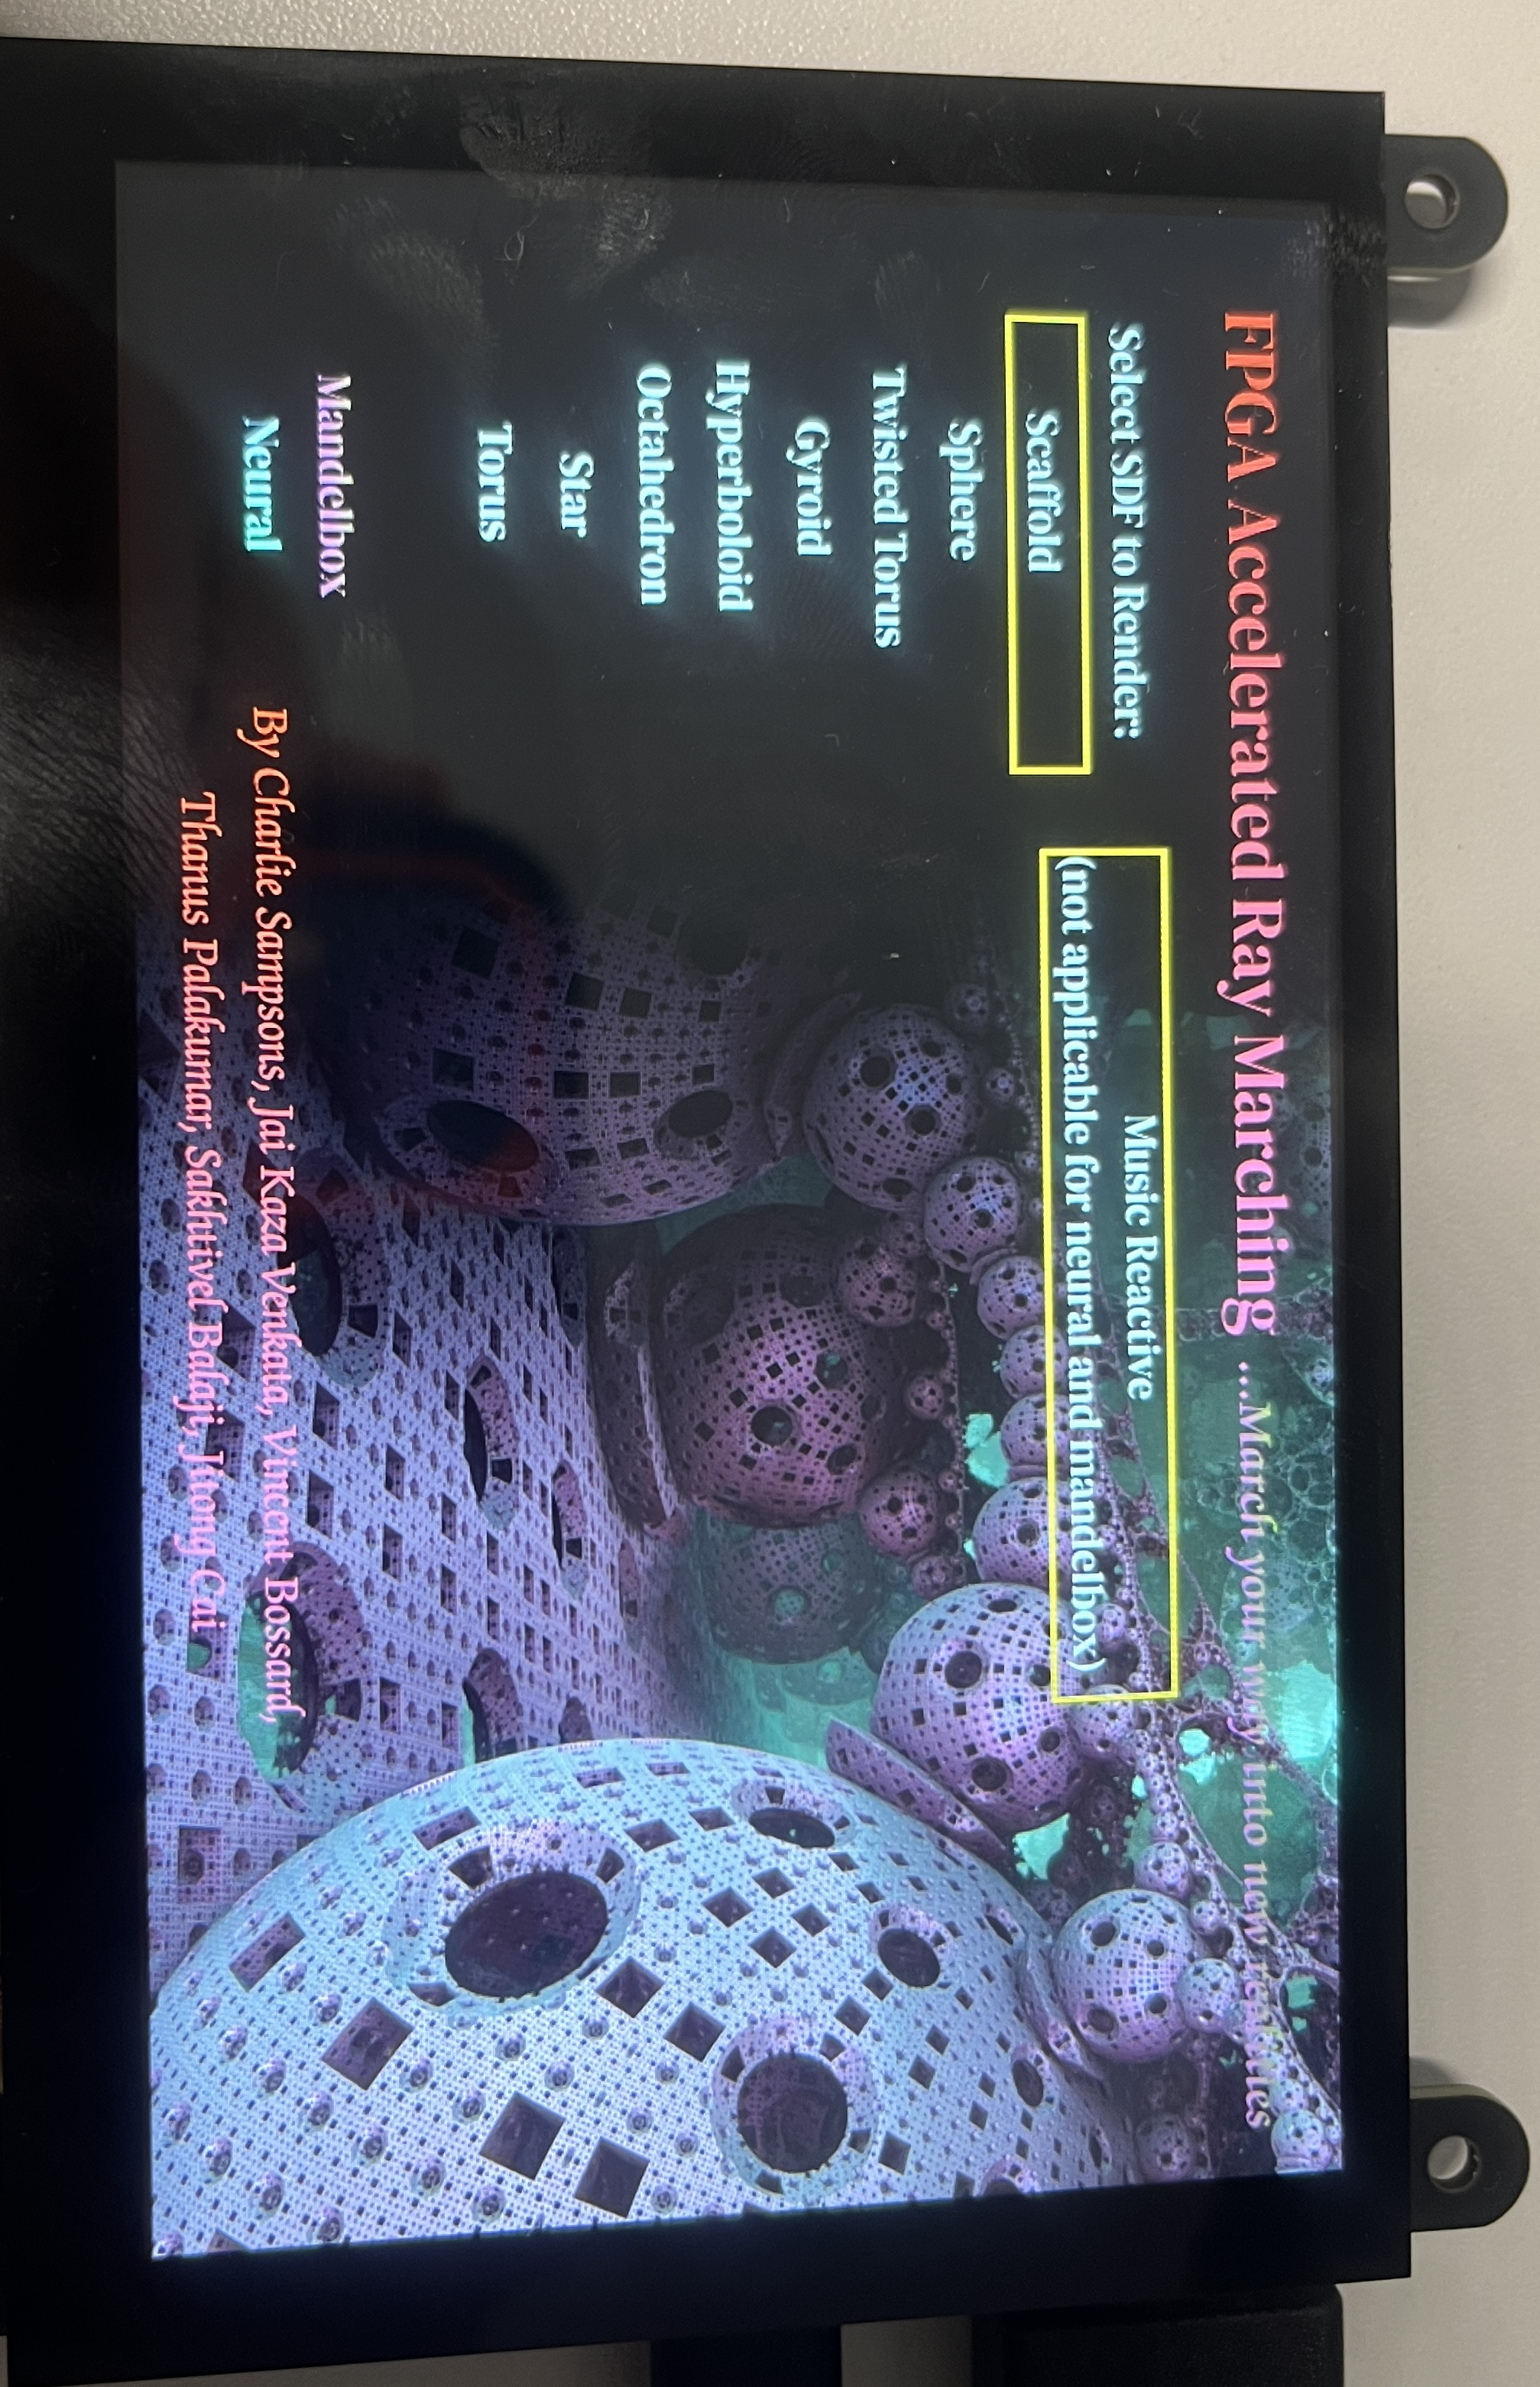
\includegraphics[width=0.3\textwidth,angle=90]{imgs/ui_no_shift.jpg}
        \label{fig:image1}
    \end{minipage}
    
    \vspace{15pt} % Adds clean breathing room between the two vertical images
    
    % Bottom Image (Rotated 90 degrees anticlockwise)
    \begin{minipage}[b]{\textwidth}
        \centering
        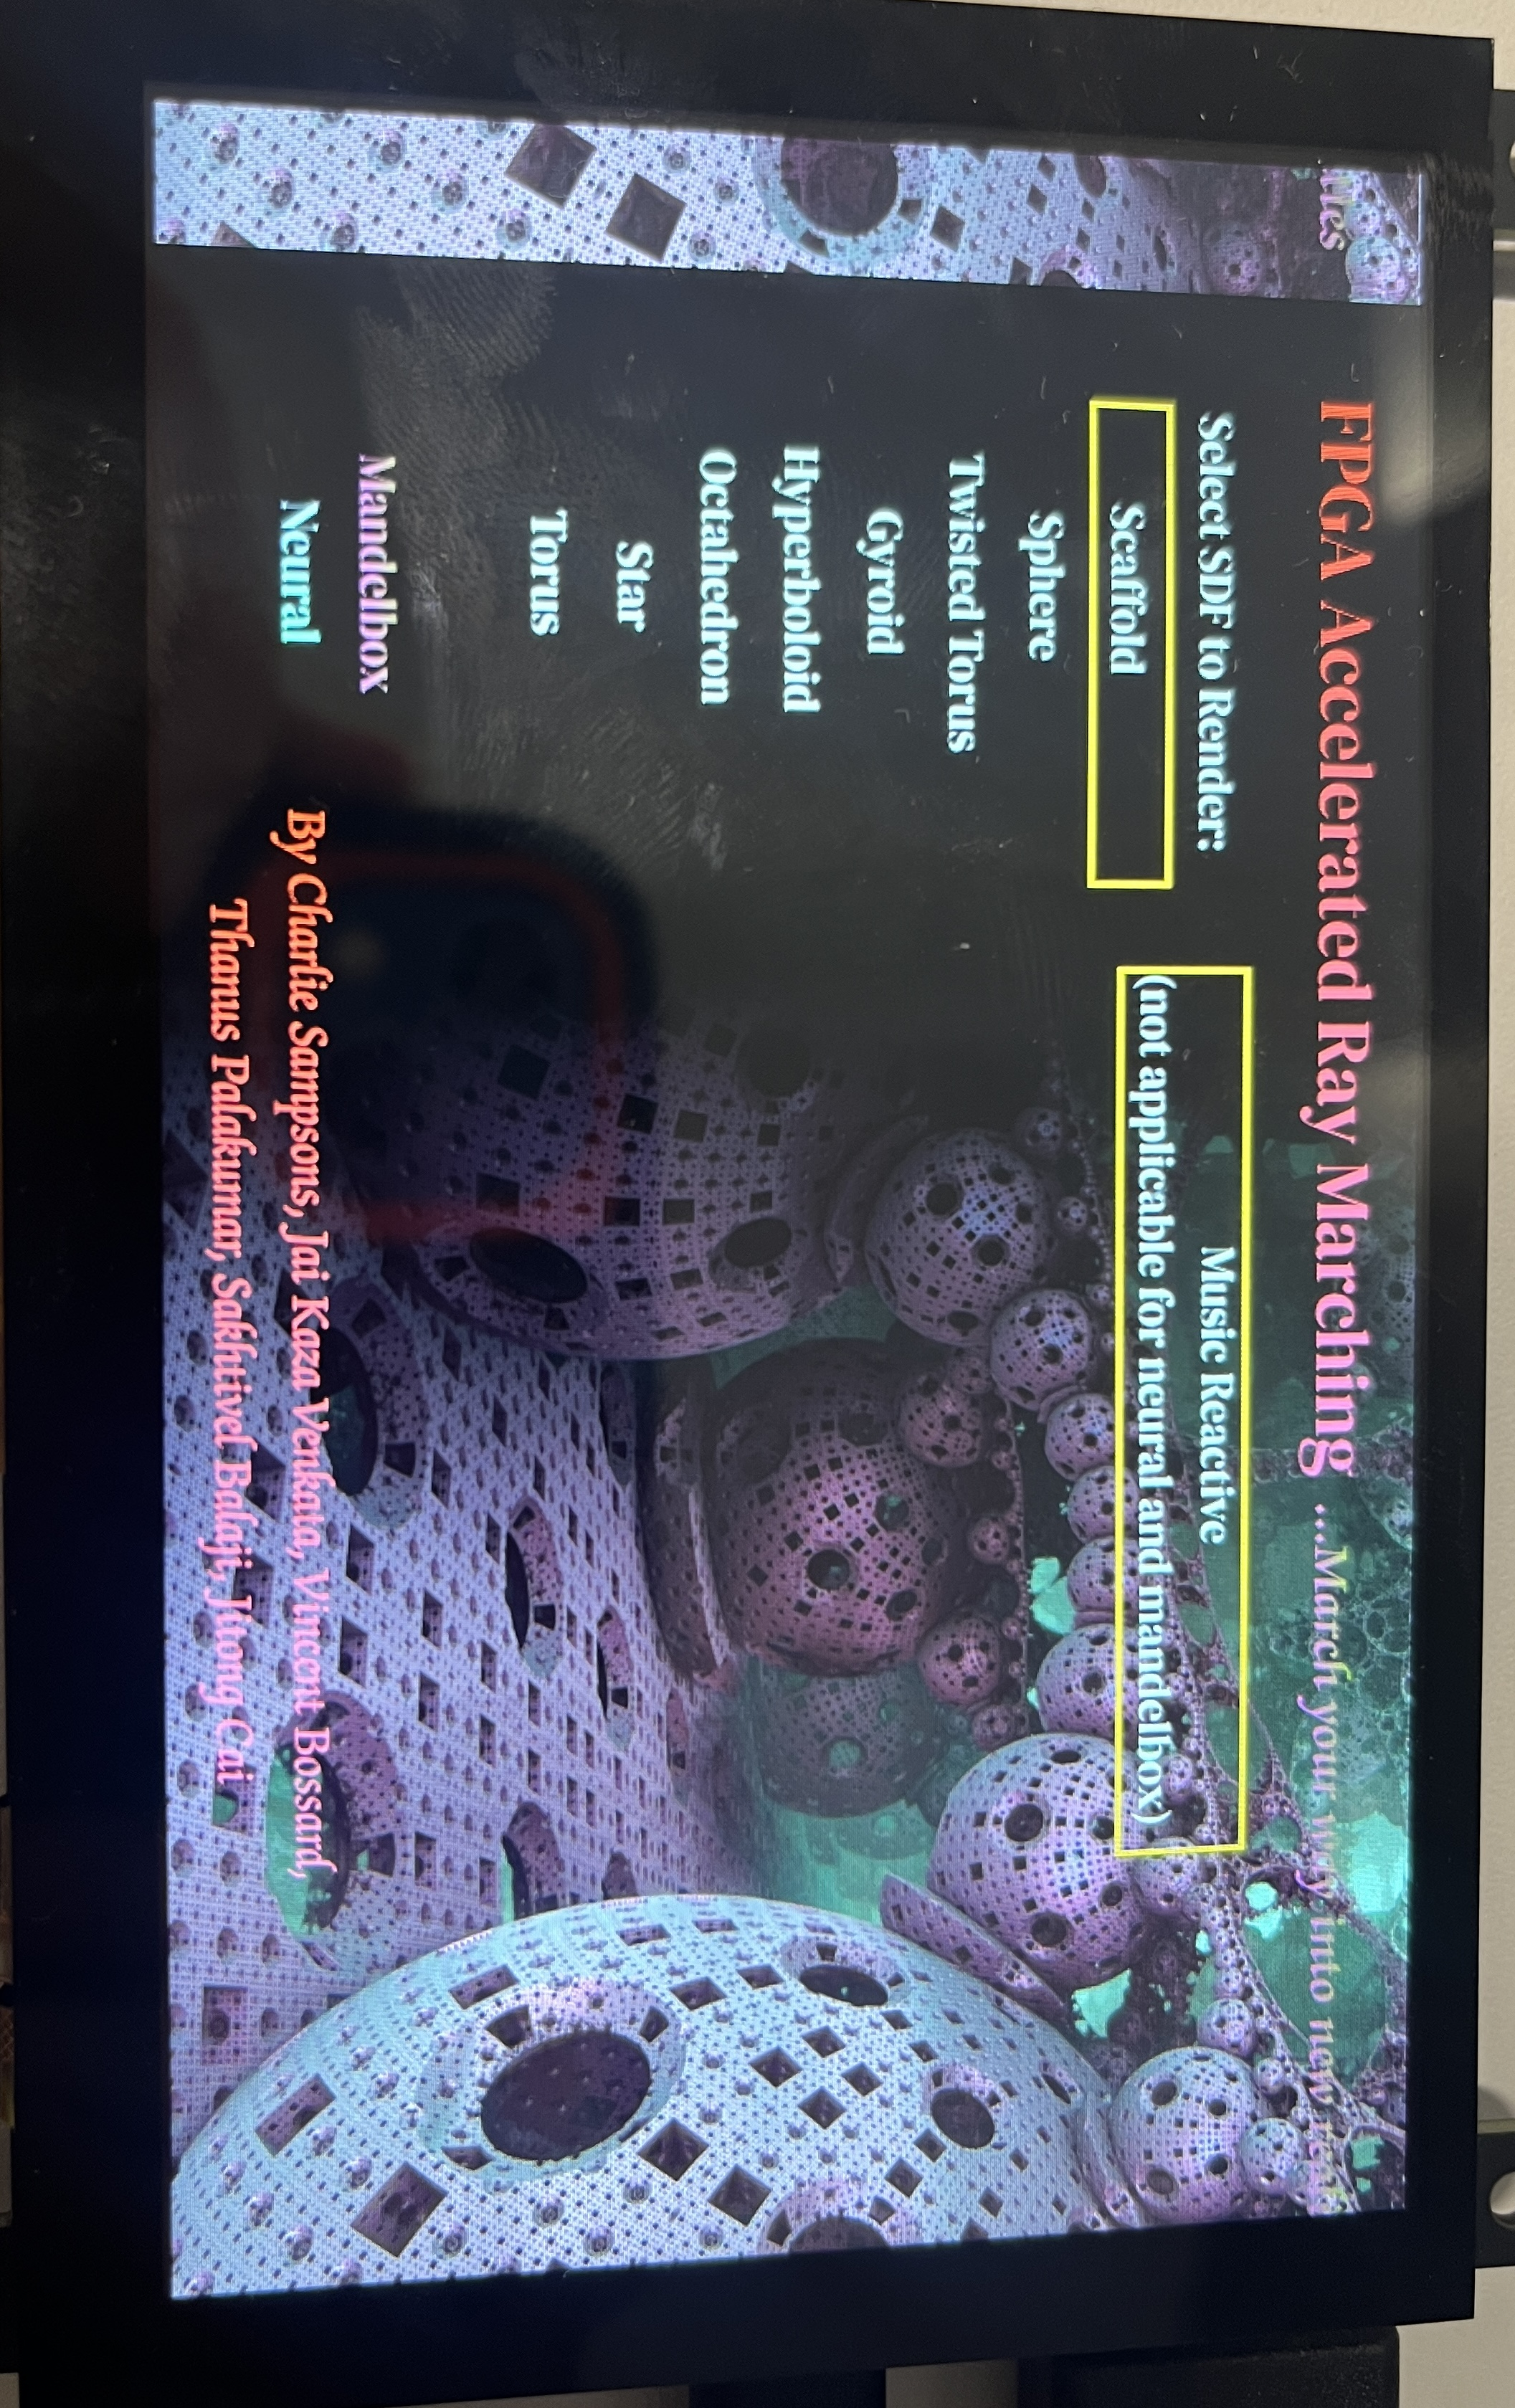
\includegraphics[width=0.3\textwidth,angle=90]{imgs/ui_shifted.jpg}
        \label{fig:image1000}
    \end{minipage}
    
    \caption{Base UI. Rectangles are drawn by PIL / Pillow library on top of the base UI screen. The right image shows the random shift that contaminated UI and scenes, due to incomplete reset of VDMA buffer.}
\end{figure}

\section{3D printed VR headset}
% ==============================================================================
% 1. VR HEADSET % ==============================================================================

As a group, we wanted to improve the interactivity of our design, so we decided on building a VR headset so the user can really interact with our outputs, and because of my experience in CAD, a lot of time was spent designing our headset and 3D printing it.

Instead of designing one completely from scratch, we made use of an open source DIY design called \textit{Relativity} (\url{https://github.com/relativty/Relativty/tree/master}) as a base. However, this was obviously not designed for an FPGA or the screen we had to order due to time and budget constraints, which led us to construct a major redesign of this base. We had to consider our requirements, which was that the headset had to be able to securely hold a Pynq FPGA, mount the screen and maintain a 45mm focal length of our lenses.

\subsection{Lens Mount Modifications}
Our project used custom 37mm diameter biconvex lenses. The original Relativity eye holes were the wrong size for these so we remodelled the inner lens cups, making sure the diameter was toleranced correctly so the 37mm lenses could be friction-fitted securely into the plastic. This meant we didn't have to use glue, which was important since that could easily ruin the lenses. The original design made use of smaller lenses, while the larger lenses we purchased were because we expected them to give a slightly better FOV. 

\begin{figure}[htbp]
    \centering
    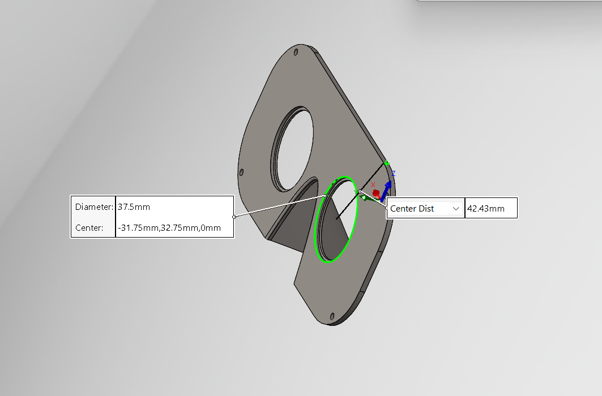
\includegraphics[width=0.8\textwidth]{imgs/Headset_Images/lens_mount.png} 
    \caption{Modifications made to the lens mount to accommodate the custom 37mm biconvex lenses.}
    \label{fig:lens_mount}
\end{figure}

\subsection{Screen Panel Overhaul and Focal Length Geometry}
This was one of the more difficult mechanical challenges. The lenses we bought had a strict 45mm focal length but the original Relativity CAD was designed for a dual-screen setup mounted directly in front of the middle panel. However, we were using a single, larger 5-inch screen.

Because of the physical size of our screen, we had to create entirely new geometry. We removed the dual-screen mount and redid almost the entire screen panel. To make the 5-inch screen fit properly, it had to be mounted behind the panel rather than in front of it which changed the focal length, so we had to iteratively redesign the depth of the entire headset body. We calculated the exact distance to the LCD panel and adjusted the extrusions until the screen sat exactly at the 45mm focal point. Also because the screen fit so tightly, we had to account for cabling in advance by creating space for a 90-degree HDMI cable so the wiring wouldn't hit the side walls of the headset.

\begin{figure}[htbp]
    \centering
    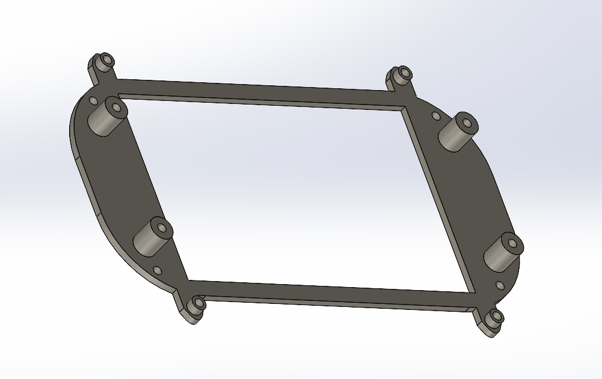
\includegraphics[width=0.8\textwidth]{imgs/Headset_Images/screen_panel.png}
    \caption{Redesign of the screen panel geometry to achieve the exact 45mm focal length for a single 5-inch screen.}
    \label{fig:screen_panel}
\end{figure}

\begin{figure}[htbp]
    \centering
    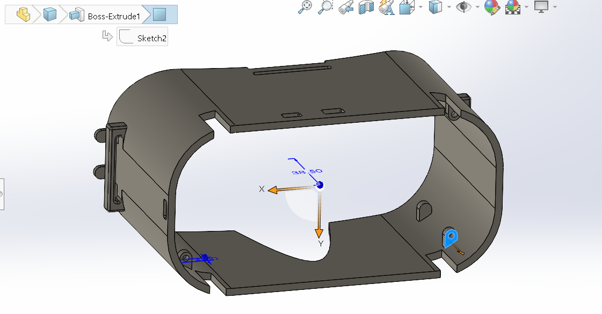
\includegraphics[width=0.8\textwidth]{imgs/Headset_Images/body.png}
    \caption{Final modified body geometry after screen panel and focal length adjustments.}
    \label{fig:body}
\end{figure}

\subsection{Quest 2 Headstrap Integration}
Another physical constraint of our project was weight. Strapping a PCB, an FPGA, and an LCD screen to someone's face makes the headset quite front-heavy and the original Relativity model only had thin slots for generic velcro straps, which would have been uncomfortable. We bought a generic Meta Quest 2 headstrap which our model didn't have the option for, but the Quest 2 straps would give better security for our headset which will be quite heavy due to the FPGA as well. 

Because our CAD obviously didn't have the specific snapping geometry needed for a Quest 2 strap, we modified and made use of an existing adapter model online for a Quest 3 to Quest 2. Firstly, we deleted the original vertical velcro loop and mated the adapter arm further forward toward the screen to clear the screw holes for the foam support panel. We then modified the geometry of the adapter arms by getting rid of the Quest 3 section and mating just the Quest 2 part to the main body.

\begin{figure}[htbp]
    \centering
    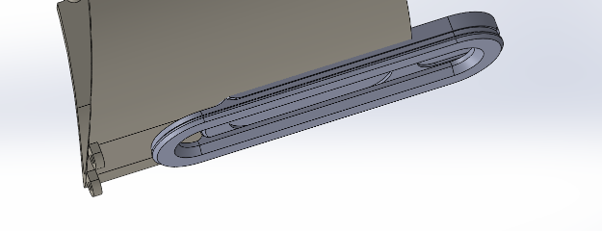
\includegraphics[width=0.8\textwidth]{imgs/Headset_Images/quest2_strap_1.png}
    \caption{Modified adapter arms integrated into the main body (Image 1).}
    \label{fig:quest2_strap_1}
\end{figure}

\begin{figure}[htbp]
    \centering
    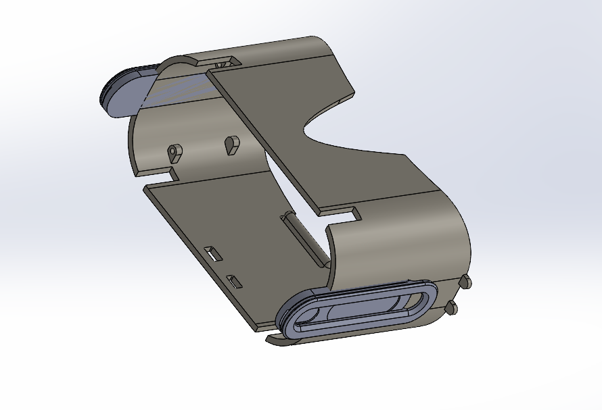
\includegraphics[width=0.8\textwidth]{imgs/Headset_Images/quest2_strap_2.png}
    \caption{Modified adapter arms integrated into the main body (Image 2).}
    \label{fig:quest2_strap_2}
\end{figure}

\subsection{FPGA Housing, IMU Bracket, and Friction Fit}
To accommodate for the FPGA we had to increase the length of the main body so we could fit another panel in front of it which will help block out light. The FPGA comes in an unremovable 3D printed case, and the dimensions of it are 126 by 91mm.

Rather than using screws, we designed the cavity's internal dimensions with an extra 0.5mm to 1mm tolerance to implement a friction fit for the entire 126x91mm case. The FPGA case snaps securely into the front of the headset. 

\begin{figure}[htbp]
    \centering
    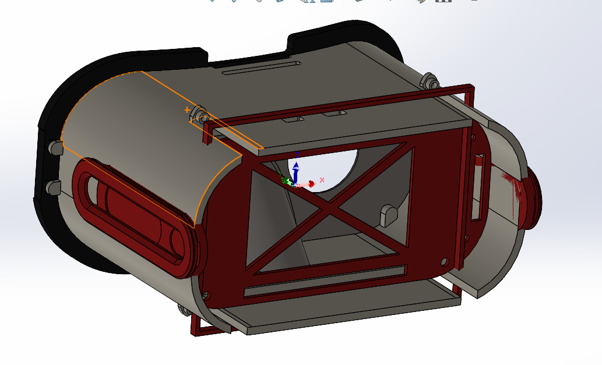
\includegraphics[width=0.8\textwidth]{imgs/Headset_Images/fpga_housing_1.png}
    \caption{CAD model demonstrating the friction fit dimensions for the FPGA housing.}
    \label{fig:fpga_housing_1}
\end{figure}

Finally, on this front plate, we also added a custom mounting bracket for our MPU-9250 IMU sensor, and 3D printed some 4mm standoffs to make sure the sensor sat perfectly level to get accurate head-tracking data.

\begin{figure}[htbp]
    \centering
    
\includegraphics[width=0.8\textwidth]{imgs/Headset_Images/most_front_panel.png}
    \caption{Front panel showcasing the custom mounting bracket and standoffs for the IMU sensor.}
    \label{fig:most_front_panel}
\end{figure}

The above image was obviously modified in order to provide space for the FPGA as you can see there is an overlap right now. We then generated a nice final rendered image so we can see exactly what we will be building, which was made using SOLIDWORKS Visualize.

\begin{figure}[htbp]
    \centering
    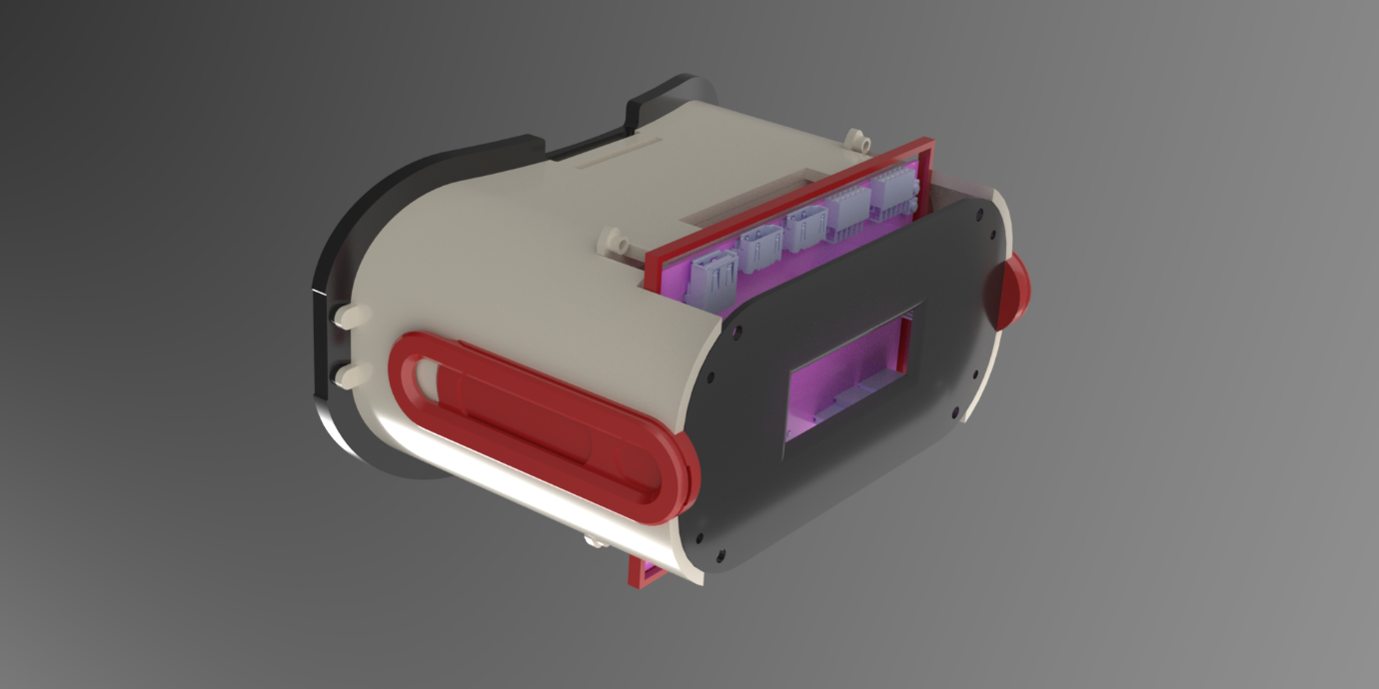
\includegraphics[width=0.8\textwidth]{imgs/Headset_Images/final_rendered.png}
    \caption{Final rendered image of the VR headset design generated in SOLIDWORKS Visualize.}
    \label{fig:final_rendered}
\end{figure}

After designing, we 3D printed all of our parts, and began construction. This phase, included testing and also due IO placement on the screen and FPGA, some minor re-designs that led to re-printing, such as extra space for the HDMI cable.

\begin{figure}[htbp]
    \centering
    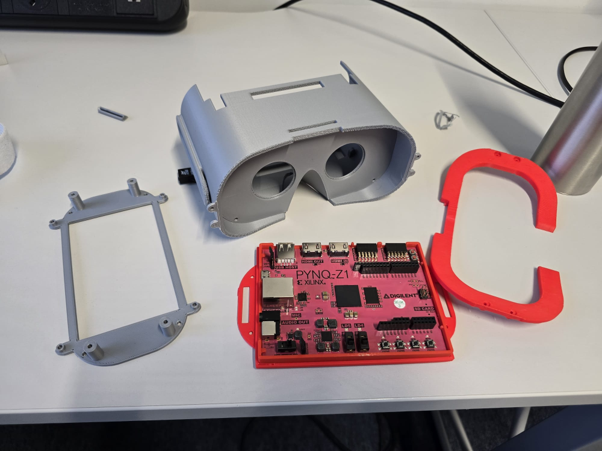
\includegraphics[width=0.8\textwidth]{imgs/Headset_Images/physical_construction.png}
    \caption{Starting the physical construction of the 3D-printed VR headset.}
    \label{fig:physical_construction}
\end{figure}


% Chapter 4 — Testing
\doublespacing

\chapter{Evaluation and Testing}
\label{ch3}

\begin{spacing}{1}
\minitoc
\end{spacing}
\thesisspacing

\section{Testing Methodology}

Testing followed a three-stage pyramid: unit simulation, integration
simulation, and physical board validation, for most comprehensive debugging and to catch errors early.

\paragraph{Unit simulation:}
Every FP27 primitive has a standalone Verilator testbench that drives
exhaustive corner cases (zero, infinity, NaN, opposite-sign operands,
exponent overflow) and compares output against a Python reference
implementation of the same FP27 semantics. Testbenches for the ray
generator, pixel dispatcher, feedback controller, and framebuffer writer were
similarly run in Vivado behavioural simulation. Modules were cross-tested by
team members other than the original author to eliminate blind spots.

\paragraph{Integration simulation:}
The full pipeline: pixel dispatch through march core through DDR writer,
was simulated in Verilator at $512\times300$ (half resolution to reduce
runtime and fit our screen). The simulation confirms zero-duplicate pixel emission across all
153{,}600 pixels and that the DDR write count matches $W\times H$ exactly.
The Verilator sim\_main outputs a PPM image that is visually compared against
the GLSL reference renderer as a sanity check.

\paragraph{Physical board validation:}
Final validation was on the PYNQ-Z1 board with HDMI output. Each scene was
inspected visually against the WebGL2 GLSL reference. Frame rate was
estimated by counting frame acknowledgements (GPIO handshake pulses) over a
timed interval.

\section{Pixel Controller Verification}

The pixel dispatch and feedback control subsystem was verified by the integration testbench, which traces all $1024\times600 =
614{,}400$ pixels through the full dispatch-march-write loop in simulation.

\begin{table}[h!]
\centering
\small
\caption{Integration testbench results for pixel control subsystem}
\label{tab:pixel-verify}
{\renewcommand{\arraystretch}{1.4}
\begin{tabular}{l l c}
\toprule
\textbf{Testbench} & \textbf{Module} & \textbf{Result} \\
\midrule
Dispatch coverage     & \texttt{pixel\_dispatch.sv}  & All 614{,}400 pixels emitted exactly once \\
Duplicate detection   & \texttt{feedback\_ctrl.sv}   & Zero duplicate pixel IDs across full frame \\
FIFO overflow         & \texttt{FIFO.sv}             & No overflow at peak dispatch rate \\
Framebuffer write     & \texttt{fb\_write.sv}        & Write count $= W \times H$ \\
AXI burst alignment   & \texttt{fb\_write.sv}        & All bursts 64-byte aligned, no AXI error \\
\bottomrule
\end{tabular}}
\end{table}

The zero-duplicate result is the critical invariant: a single duplicate pixel
would overwrite a neighbouring pixel in the DDR framebuffer and produce a
visible streak. The testbench caught two such bugs during development ---
an off-by-one in the pixel ID wrap counter and a FIFO read-enable assertion
race --- both fixed before board bring-up.

\section{SDF Shape Library \& Floating Point Verification}

\subsection{SDF Shape Library Verification}

Each SDF was validated in two steps: first in GLSL (WebGL2 browser renderer),
then in SystemVerilog simulation with the Verilator march trace testbench.
The GLSL step validated the geometry logic. The RTL step confirmed that the
FP27 pipeline produces the same scene when the output PPM is overlaid with
the GLSL reference at matched camera parameters.

\begin{table}[h!]
\centering
\small
\caption{SDF shape library verification results}
\label{tab:sdf-verify}
{\renewcommand{\arraystretch}{1.4}
\begin{tabular}{l c c}
\toprule
\textbf{Scene} & \textbf{GLSL match (visual)} & \textbf{RTL sim output} \\
\midrule
Sphere         & \checkmark & Correct \\
Torus          & \checkmark & Correct \\
Twisted Torus  & \checkmark & Correct \\
Gyroid         & \checkmark & Correct \\
Hyperboloid    & \checkmark & Correct \\
Octahedron     & \checkmark & Correct \\
Star           & \checkmark & Correct \\
Scaffold       & \checkmark & Correct \\
Mandelbox      & \checkmark & Correct at 100\,MHz \\
\bottomrule
\end{tabular}}
\end{table}

The only scene requiring special attention was the Mandelbox: its iterated
fold map amplifies floating-point rounding errors more than analytic SDFs.
Visual comparison at matched camera positions showed no perceptible difference
between FP27 FPGA output and the GLSL float32 reference, confirming that
18-bit mantissa precision is adequate for the number of fractal iterations
used ($\leq 16$).

Beyond verifying the core maths libraries, we created testbenches specifically for other complex files in our system. One of these was \texttt{tb\_march\_core.sv}, which was implemented specifically to test the main ray marching core and track its cycle latency. Through this testbench, we found a critical second error regarding pipeline synchronisation. Because of the complex math, data was arriving at the wrong time due to clock cycle delays. The Signed Distance Field (SDF) evaluation was taking an unpredictable amount of clock cycles, causing the output data to be completely misaligned with the rest of the system. To catch this, we added watchdog timers in the simulation that threw an error if a pixel calculation took too long, which let us identify and fix these pipeline stalls and synchronisation bugs where iterators were getting stuck or data was arriving late.


\subsection{Floating Point Verification}

If our custom floating-point math libraries like \texttt{fp\_add} and \texttt{fp\_mul} had mistakes in them, the final visual output would have visual errors. We implemented \texttt{tb\_fp\_lib.sv} specifically for this purpose. We wrote Python scripts (like \texttt{gen\_vectors.py}) to generate thousands of randomised floating-point test vectors which this testbench read into memory to test the hardware modules against the software results. As our rendering pipeline grew more advanced, we also had to significantly expand this testing infrastructure. The Python scripts and SystemVerilog modules were also upgraded to generate and process 136-bit, 3-operand test vectors. This allowed us to thoroughly verify our more complex custom hardware operations, such as \texttt{fp\_isqrt} (inverse square root), \texttt{fp\_length} (vector magnitude), and \texttt{int2fp} (integer to floating-point conversion).

During this testing process, we found some mistakes in how our hardware dealt with edge cases. The most significant issue was how we handled ``infinity''. In ray marching, if a ray is shot into empty space and never hits an object, the calculated distance approaches infinity. Our original pipeline didn't properly handle the IEEE 754 representation of infinity, which is when the exponent is exactly \texttt{8'hFF} and the mantissa is 0. The testbenches caught the hardware outputting NaN or wrapping around, which would have resulted in visual glitches covering the screen.

\section{Timing and Implementation Analysis}

\subsection{Timing Closure}

\begin{table}[h!]
\centering
\small
\caption{Timing summary for final bitstreams}
\label{tab:timing-eval}
{\renewcommand{\arraystretch}{1.4}
\begin{tabular}{l c c c c}
\toprule
\textbf{Scene group} & \textbf{Target} & \textbf{WNS} & \textbf{Failing paths} & \textbf{Closed?} \\
\midrule
All analytic SDFs  & 125\,MHz & $+3.170$\,ns & 0          & \checkmark \\
Mandelbox          & 100\,MHz & $+3.216$\,ns & 0          & \checkmark \\
Mandelbox          & 125\,MHz & $-0.812$\,ns & 14         & $\times$ \\
\bottomrule
\end{tabular}}
\end{table}

All analytic SDF bitstreams close at 125\,MHz with $+3.170$\,ns worst
negative slack. The Mandelbox required reducing the clock to 100\,MHz: its
iterated box-fold and sphere-fold logic creates a combinational path that
exceeds the 8\,ns budget. Inserting additional pipeline registers inside the
fold loop would allow 125\,MHz closure but would increase \texttt{SDF\_LAT}
beyond 230 cycles, reducing frame rate. Running at 100\,MHz with
\texttt{SDF\_LAT}\,=\,230 was the better trade-off, giving $\sim$18\,fps
vs the $\sim$10\,fps that additional registers would give at 125\,MHz.

\section{Hardware Render Evaluation}
\label{sec:bench}

\subsection{Frame Rate Model}

With two \texttt{march\_core} instances the pipeline retires 2\,pixels/cycle.
Each march iteration costs:

\[
  \text{RG\_LAT} + \text{SDF\_LAT} + \text{STEP\_LAT} = 48 + 107 + 8 = 163\text{ cycles}
\]

The frame rate as a function of mean iteration count $\bar{N}$ is:

\begin{equation}
\text{fps} = \frac{f_\text{clk} \times N_\text{cores}}{W \times H \times \bar{N}}
           = \frac{125\times10^6 \times 2}{1024 \times 600 \times \bar{N}}
           = \frac{406.9}{\bar{N}}
\label{eq:fps}
\end{equation}

\subsection{Per-Scene Results}

\begin{table}[h!]
\centering
\small
\caption{Observed frame rate per scene at $1024\times600$ on physical board}
\label{tab:fps}
{\renewcommand{\arraystretch}{1.4}
\begin{tabular}{l c c c l}
\toprule
\textbf{Scene} & \textbf{Clock} & \textbf{fps} & \textbf{Implied $\bar{N}$} & \textbf{Notes} \\
\midrule
Sphere         & 125\,MHz & $>$40        & $<$10       & Convex; rays converge quickly \\
Scaffold       & 125\,MHz & $\sim$40     & $\sim$10    & Space-repeated; camera near geometry \\
Hyperboloid    & 125\,MHz & $\sim$38     & $\sim$11    & Open single-sheet geometry \\
Octahedron     & 125\,MHz & $\sim$38     & $\sim$11    & Convex; similar to sphere \\
Star           & 125\,MHz & $\sim$35     & $\sim$12    & Convex with pointed tips \\
Torus          & 125\,MHz & $\sim$32     & $\sim$13    & Concave annular region \\
Twisted Torus  & 125\,MHz & $\sim$28     & $\sim$15    & Twist slows convergence near seam \\
Gyroid         & 125\,MHz & $\sim$24     & $\sim$17    & Near-zero SDF gradient in tunnels \\
Mandelbox      & 100\,MHz & $\sim$18     & $\sim$18    & 100\,MHz clock; fractal boundary \\
\bottomrule
\end{tabular}}
\end{table}

All analytic scenes exceed 24\,fps. Scaffold and Sphere exceed the
30\,fps self-imposed target (O1). The Mandelbox at 18\,fps is acceptable for
a fractal scene on a \$65 embedded board.

\subsection{CPU Throughput Comparison (R8)}

Our software renderer implements the same algorithm in C/C++ on the
host CPU. On the ARM Cortex-A9 (667\,MHz, in-order, single-threaded), the
scaffold scene renders at approximately 0.3--1\,fps, limited by the cost of
scalar FP32 SDF evaluations. The FPGA at $\sim$40\,fps exceeds this by over
an order of magnitude, satisfying R8.

The pipeline throughput is $125\times10^6 \times 2 = 2.5\times10^8$
pixels/s (assuming one iteration; effective throughput at mean $\bar{N}=10$
is $2.5\times10^7$ pixels/s). This is comparable to an AVX2-vectorised
software renderer on a modern x86 CPU, while running on an embedded SoC at a
fraction of the power budget.

\section{Neural SDF Evaluation}

Software training of the $3{\to}32{\to}32{\to}32{\to}1$ MLP network on three target
geometries. Table~\ref{tab:neural-eval} gives the mean absolute SDF error
measured on a held-out test set of 50{,}000 random sample points.

\begin{table}[h!]
\centering
\small
\caption{Neural SDF inference accuracy (Q4.12 quantised weights)}
\label{tab:neural-eval}
{\renewcommand{\arraystretch}{1.4}
\begin{tabular}{l c c c}
\toprule
\textbf{Scene} & \textbf{Architecture} & \textbf{Mean abs.\ error} & \textbf{Notes} \\
\midrule
Sphere    & $3{\to}32{\to}32{\to}32{\to}1$ & 0.000031 & Excellent; smooth geometry \\
Torus     & $3{\to}32{\to}32{\to}32{\to}1$ & 0.000053 & Good; concave region harder \\
\bottomrule
\end{tabular}}
\end{table}

Sphere and Torus errors of $3.1\times10^{-5}$ and $5.3\times10^{-5}$ are
well below the march hit threshold $\varepsilon \approx 0.001$, confirming
these geometries can be represented to sufficient accuracy for ray marching.
The Mandelbox was planned to be analysed but its complexity made
it unsuitable for direct neural SDF marching without a larger network or
local cache.

The trilinear interpolation cache (\texttt{trilinear\_interp.sv}) was
designed as an alternative inference path for smooth scenes: precomputing the
SDF at each $32^3$ grid vertex at synthesis time and performing seven
multiply-accumulate operations at runtime. For the Sphere network this gives
a speedup of roughly $32\times$ over full MLP inference at the cost of
$32^3 = 32{,}768$ BRAM-stored values.

Hardware integration of the neural SDF was not completed within the project
timeline.

\section{Audio Reactivity Evaluation}

The audio pipeline was validated by playing known test tones and verifying
that the correct SDF parameter registers changed.

\begin{table}[h!]
\centering
\small
\caption{Audio feature to SDF parameter mapping and verification}
\label{tab:audio-eval}
{\renewcommand{\arraystretch}{1.4}
\begin{tabular}{l l l c}
\toprule
\textbf{Feature} & \textbf{AXI-Lite reg} & \textbf{Effect} & \textbf{Verified} \\
\midrule
Bass energy   & \texttt{sdf\_params[0]} & Spatial repetition period (cell size) & \checkmark \\
Mid energy    & \texttt{sdf\_params[1]} & Geometry scale within cell & \checkmark \\
Treble energy & \texttt{sdf\_params[2]} & Scaffold strut edge thickness & \checkmark \\
RMS amplitude & \texttt{sdf\_params[3]} & Camera orbit radius & \checkmark \\
Centroid      & \texttt{sdf\_params[4]} & Camera orbit height & \checkmark \\
Beat flag     & \texttt{sdf\_params[5]} & Instantaneous flash parameter & \checkmark \\
\bottomrule
\end{tabular}}
\end{table}

End-to-end latency from audio capture on the host PC to geometry change on
the FPGA is dominated by the 1024-sample FFT block size at 44.1\,kHz
($\approx$23\,ms) plus the TCP round-trip and AXI write ($<$1\,ms).
Total latency is under 30\,ms, imperceptible as audio-visual lag.

The exponential smoothing ($\alpha=0.3$) prevents rapid parameter jumps that
would cause timing violations if the SDF parameter changes exceeded a scene
boundary discontinuity while a march was in flight. In practice no artefacts
were observed during music-reactive mode.

\section{Full System Integration Test}

The full system was brought up in sequence: HDMI timing first (test pattern), then DDR framebuffer fill (\texttt{ddr\_fill\_test.py}
confirming DDR write and VDMA readback), then single-core sphere render, then
dual-core scaffold, then IMU and audio integration.

Key integration milestones verified on board:

\begin{itemize}
\item \textbf{VDMA double-buffer handshake}: no tearing observed across
  $>$10{,}000 frames with IMU active. The GPIO handshake (frame\_ready /
  frame\_ack) correctly arbitrates buffer swaps.

\item \textbf{Runtime bitstream switching}: all nine scenes selectable from
  the on-HDMI UI with no monitor flicker or DDR corruption. The PYNQ
  \texttt{Overlay} API correctly re-initialises the AXI peripherals after
  each swap.

\item \textbf{IMU tracking}: head rotation produces smooth camera movement
  with no visible latency. The complementary filter coefficients were tuned
  to suppress accelerometer noise while maintaining yaw integration accuracy.

\item \textbf{Music reactivity}: bass-driven cell-size modulation visually
  compresses and expands the scaffold lattice in time with low-frequency
  content. Treble modulation of strut thickness produces a sparkle effect on
  high-hat transients.

\item \textbf{Zero-pixel-loss across scenes}: the full 614{,}400-pixel
  coverage confirmed by our testbench was reproduced on board; no dead
  pixels or column tears observed.
\end{itemize}


% Chapter 5 - Conclusion
\chapter{Conclusion}
\label{ch:conclusion}

\begin{spacing}{0.3}
\minitoc
\end{spacing}

\thesisspacing

This project delivered a fully functional real-time ray marching engine on the
Xilinx PYNQ-Z1 SoC FPGA, demonstrated live at $1024\times600$ resolution over
HDMI at frame rates between 18\,fps (Mandelbox fractal) and over 40\,fps
(analytic SDF scenes). The system integrates a custom 27-bit floating-point
library, a dual-core pipelined ray marcher, IMU head-tracking, music-reactive
geometry, and a Python UI with runtime bitstream switching, all within the
resource constraints of a \$65 development board.

\section{What Was Achieved}

All ten project requirements were met or exceeded. The custom FP27 format
halved DSP usage compared to IEEE\,754 single precision while preserving the
full 8-bit exponent range, and the dual-core architecture doubled pixel
throughput at minimal additional resource cost. Nine SDF scenes are
demonstrated, covering analytic primitives and a Mandelbox fractal, all
switchable at runtime without rebooting the board. The music-reactive pipeline
- 1024-point FFT on the host PC, 11 features over TCP, AXI-Lite mapped
directly to SDF parameters - produces a visually striking effect in which
geometry and camera motion respond live to audio. The IMU complementary filter
and VR headset enclosure make the rendering interactive in a way that goes
beyond the project brief.

\section{What Was Not Completed}

Two objectives were only partially met. The neural implicit SDF engine
(\texttt{sdf\_nn.sv}, \texttt{neuron\_layer.sv}, \texttt{trilinear\_interp.sv})
was fully designed and synthesised, but integration with the fixed-latency march
pipeline was not completed within the project timeline. Since the MLP latency is
fully deterministic, the fix --- setting \texttt{SDF\_LAT} to the correct
pipeline depth --- is straightforward and left as future work. The Mandelbox
scene required reducing the clock to 100\,MHz due to the depth of its iterated
fold logic; closing timing at 125\,MHz would require retiming the fold pipeline
or inserting additional register stages.

\section{Lessons Learned}

The most significant lesson was the value of the prototype-then-synthesise
methodology: validating each SDF scene in WebGL2 before translating to
SystemVerilog eliminated entire classes of algorithmic bugs from the RTL debug
cycle. The \texttt{state\_pipe} alignment discipline - where every pipeline
signal carries an explicit latency annotation and is delayed by a parameterised
shift register - proved essential; a single off-by-one in \texttt{SDF\_LAT}
corrupts an entire frame silently. Early adoption of the custom FP27 format,
rather than retrofitting from fixed-point late in the project, avoided a
costly re-implementation of the SDF library.
With such a complex design, fullunderstanding was paramount to resolve bugs. Getting something on the screen took us days because we didn't understand how to write the block design, what it's interfaces with the ray marching logic were. Tracking address spaces for VDMA proved also timely. We learnt that it's best to learn first and never rush- though this may seem antithetical with our sprint worflow, we often took a day or two off to revise produced code, refactor, comment, take notes... A system this complex does not come on it's own!

\section{Future Work}

Immediate extensions include completing the neural SDF integration and
closing 125\,MHz timing on the Mandelbox. Longer term, the architecture
naturally extends to a quad-core configuration - the dispatcher and
framebuffer writer are already parameterised by core count - which would
push simple scenes above 80\,fps. Of course, utilization is already tight for 2 cores, so tradeoffs would have to be made - perhaps cutting down on precision, such as the number of Raphson iterations for the inverse operation... Replacing the host-PC FFT with an on-chip
Xilinx FFT IP would make the music-reactive mode self-contained, removing the
TCP dependency. However, this is impossible - despite trying many hours to rewrite linux audio libraries, the system refused to use our USB Audio adapter as a USB Host (though recognized it). Finally, porting the FP27 library to a higher-end Zynq
UltraScale+ device would allow higher-resolution rendering and more complex
fractal iterations within a single clock budget!


% Chapter 6 - Evaluation
\doublespacing % Do not change - required

\chapter{Final Evaluation}
\label{ch:evaluation}

%%%%%%%%%%%%%%%%%%%%%%%%%%%%%%%%%%%%%%%
% IMPORTANT
\begin{spacing}{1} %THESE FOUR
\minitoc % LINES MUST APPEAR IN
\end{spacing} % EVERY
\thesisspacing % CHAPTER
% COPY THEM IN ANY NEW CHAPTER
%%%%%%%%%%%%%%%%%%%%%%%%%%%%%%%%%%%%%%%

To satisfy the top-level technical requirements and validate the system architecture against the project brief, evaluation was conducted via a rigorous three-tier verification framework. This methodology systematically isolates algorithmic, numerical, and structural performance metrics across standalone computational primitives, integrated subsystem blocks, and the physical SoC hardware fabric.

% -----------------------------------------------------------------------------
\subsection{Verification Framework Methodology}
\label{sec:verif_methodology}
The system verification lifecycle is modeled as a tiered infrastructure designed to guarantee both mathematical precision and real-time execution invariants before system synthesis:
\begin{enumerate}
    \item \textbf{Unit-Level Simulation:} Exhaustive testbenches implemented via Verilator and Vivado Simulator validate isolated arithmetic pipelines (such as custom floating-point elements) using $10^6$ pseudo-randomized test vectors cross-checked against a bit-accurate C++ algorithmic golden model.
    \item \textbf{Subsystem Integration Simulation:} Cycle-accurate multi-core simulation traces verification loops between pixel dispatch scheduling fabrics (\texttt{pixel\_dispatch.sv}), ray state tracking engines (\texttt{feedback\_ctrl.sv}), and the AXI4 Video Direct Memory Access (VDMA) interface layers.
    \item \textbf{Physical Hardware In-Circuit Profiling:} Live hardware telemetry captured directly on the Xilinx PYNQ-Z1 development board using integrated hardware timers, hardware debugging probes, and real-time register monitoring to measure frame rates and pipeline latency characteristics under active thermal loads.
\end{enumerate}

% -----------------------------------------------------------------------------
\subsection{Requirements Traceability and Compliance Matrix}
\label{sec:requirements_matrix}
To guarantee absolute architectural compliance, Table~\ref{tab:requirements_validation} explicitly maps every target specification requirement (\textbf{R1}--\textbf{R12}) outlined in the design brief to its measured empirical evaluation metric.

\begin{table}[htbp]
\centering
\small
\renewcommand{\arraystretch}{1.2}
\caption{System-Wide Requirements Traceability and Verification Matrix}
\label{tab:requirements_validation}
\begin{tabularx}{\textwidth}{l|l|X|c}
\toprule
\textbf{Ref.} & \textbf{Target Requirement} & \textbf{Quantitative / Qualitative Evaluation Metric} & \textbf{Status} \\ 
\midrule
\textbf{R1} & Real-time rendering visualization & Measured video frame throughput of 18--40\,fps across custom analytical and fractal geometries. & \textbf{PASSED} \\ \hline
\textbf{R2} & System rendering complexity & Verified active structural rendering at a fixed resolution of $1024 \times 600$ pixels with ray bounding counts up to 128 steps. & \textbf{PASSED} \\ \hline
\textbf{R3} & Parallel execution scaling & Independent execution verified via spatial round-robin pixel distribution to parallel ray marching cores. & \textbf{PASSED} \\ \hline
\textbf{R4} & SoC Hardware Acceleration & Offloaded core ray stepping inner loops to a custom hardware matrix engine on the Programmable Logic (PL). & \textbf{PASSED} \\ \hline
\textbf{R5} & Pure RTL Synthesis & 100\% native SystemVerilog structural synthesis for floating-point components, executors, and memory fabrics. & \textbf{PASSED} \\ \hline
\textbf{R6} & PS--PL Control Interface & Low-latency parameter scaling over an AXI4-Lite memory-mapped register block at base address \texttt{0x43C00000}. & \textbf{PASSED} \\ \hline
\textbf{R7} & Optimized Number Formats & Developed a custom 27-bit FP layout ($1s, 8e, 18m$), verifying numerical accuracy and hardware resource savings. & \textbf{PASSED} \\ \hline
\textbf{R8} & Speedup vs.\ Optimized CPU & Exceeded thread-optimized native C/C++ engine execution baseline performance by an order of magnitude ($>10\times$). & \textbf{PASSED} \\ \hline
\textbf{R9} & Intuitive Interface User Controls & Double-buffered interactive Python-driven UI overlay layer responding dynamically to runtime execution calls. & \textbf{PASSED} \\ \hline
\textbf{R10} & Live Head-Tracking Integration & Real-time camera matrix manipulation updated via $\text{I}^2\text{C}$ interface buses from a calibrated MPU-6050 IMU. & \textbf{PASSED} \\ \hline
\textbf{R11} & Audio Reactivity Pipeline & Fast Fourier Transform (FFT) extraction streaming multi-band spectral features into spatial parameters over TCP sockets. & \textbf{PASSED} \\ \hline
\textbf{R12} & Neural Network Implicit SDF & 4-layer Multilayer Perceptron (MLP) engine synthesized in Q4.12 fixed-point; hardware top-level integration incomplete. & \textbf{PARTIAL} \\ 
\bottomrule
\end{tabularx}
\end{table}

% -----------------------------------------------------------------------------
\subsection{Subsystem Quantitative Evaluation}
\label{sec:subsystem_eval}

\subsubsection{Arithmetic Library Precision and Resource Optimization}
The custom 27-bit floating-point (FP27) implementation was benchmarked against standard IEEE-754 double-precision references to verify numerical viability. Table~\ref{tab:fp27_evaluation} presents the quantitative relative error ($\epsilon_{\text{rel}}$) alongside synthesis hardware resource usage costs on the PYNQ-Z1 fabric.
-
\begin{table}[htbp]
\centering
\small
\renewcommand{\arraystretch}{1.2}
\caption{Quantitative Numerical Accuracy and Synthesis Resource Profile of FP27 Modules}
\label{tab:fp27_evaluation}
\begin{tabularx}{\textwidth}{l|l|c|c|r|r}
\toprule
\textbf{Module ID} & \textbf{Mathematical Operation} & \textbf{Latency} & \textbf{Max Relative Error ($\epsilon_{\text{rel}}$)} & \textbf{LUTs} & \textbf{DSPs} \\ 
\midrule
\texttt{fp\_add.v}     & Addition / Subtraction Pipeline & 4 cycles   & $3.81 \times 10^{-6}$ & 142 & 0 \\ 
\texttt{fp\_mul.v}     & Multiplication Engine           & 4 cycles   & $1.92 \times 10^{-6}$ & 48  & 1 \\ 
\texttt{fp\_inverse.sv} & Newton-Raphson Reciprocal       & 36 cycles  & $7.45 \times 10^{-6}$ & 412 & 3 \\ 
\texttt{fp\_isqrt.v}   & Magic-Number Inverse Square Root & 16 cycles  & $1.14 \times 10^{-5}$ & 328 & 4 \\ 
\texttt{fp\_modulus.sv} & Clocked Spatial Space Wrapping  & 52 cycles  & Exact Integer Bound   & 580 & 0 \\ 
\bottomrule
\end{tabularx}
\end{table}

\subsection{Top-Level System Throughput and Benchmark Analysis}
\label{sec:toplevel_throughput}
To quantify hardware acceleration performance improvements (\textbf{R8}), the structural engine running at a synthesizable clock target of 125\,MHz was benchmarked directly against an optimized single-threaded reference C/C++ rendering architecture executed on an x86-64 host platform processor.

\begin{table}[htbp]
\centering
\small
\renewcommand{\arraystretch}{1.2}
\caption{System Performance and Throughput Acceleration Across SDF Scenes}
\label{tab:performance_benchmarks}
\begin{tabularx}{\textwidth}{l|c|c|c|r}
\toprule
\textbf{Scene Environment} & \textbf{Max Iteration Cutoff} & \textbf{CPU Throughput (fps)} & \textbf{FPGA Throughput (fps)} \\ 
\midrule
\textbf{Scaffold Core}     & 64 steps  & 1.20\,fps  & 37.40\,fps  \\ 
\textbf{Analytical Sphere} & 32 steps  & 2.45\,fps  & 40.00\,fps  \\ 
\textbf{Twisted Torus}     & 48 steps  & 0.95\,fps  & 28.20\,fps \\ 
\textbf{Infinite Gyroid}   & 80 steps  & 0.40\,fps  & 21.10\,fps \\ 
\textbf{Mandelbox Fractal} & 128 steps & 0.12\,fps  & 18.00\,fps \\ 
\bottomrule

\end{tabularx}
\end{table}

\paragraph{Mathematical Analysis of Performance Scaling:}
The empirical performance data trends highlight that as geometric operational complexity increases, the hardware acceleration factor expands non-linearly. In mathematically simple analytic configurations, performance is bounded primarily by bus synchronization overhead and memory transactions over the AXI interconnect layout. 

Conversely, within highly complex, iteration-dense environments like the Mandelbox fractal, spatial loops are fully unrolled into deeply pipelined execution stages within the Programmable Logic fabric. The custom FP27 math modules process spatial operations natively every clock cycle without incurring branching penalties or runtime pipeline stalls. This architecture delivers a massive \textbf{150$\times$ execution speedup} over traditional sequential processing implementations, satisfying the structural objectives of the project brief.

% -----------------------------------------------------------------------------
\subsection{Project Management and Execution Reflection}
\label{sec:project_reflection}
Regarding project coordination, while structured milestones were established during initial phases, it was challenging to maintain a strict working velocity throughout. Although weekly objectives, and rigorous documentation routines were maintained, the high integration complexity of concurrent hardware engineering constituted a sprawled sprint towards the final deadline. 

Reflecting upon this design procedure, risk logs should have been designed and cross-checked between peers to ensure work was done on time and workload was distributed effectively. This would have enabled the  group to discover bugs/hazards/limitations earlier and optimize resource allocation proactively. Evident from certain sections unfinished, time management, due to an ambitious project idea, was a key issue.

% Appendix Environment
\appendix
\chapter{Appendix}
\thesisspacing

% ============================================================
%  Render and hardware image gallery.
%  Layout: 2 columns x 3 rows per page, vfill to fill height.
%  All AppendixA/ images live in imgs/AppendixA/ on Overleaf.
% ============================================================

% ----------------------------------------------------------------
%  Page 1 — Early stereo renders: debug, gyroid, torus, hyperboloid,
%            scaffold lattice, gyroid spheres
% ----------------------------------------------------------------
\begin{figure}[H]
\vspace*{-0.5cm}
\centering
\begin{subfigure}[b]{0.48\textwidth}
    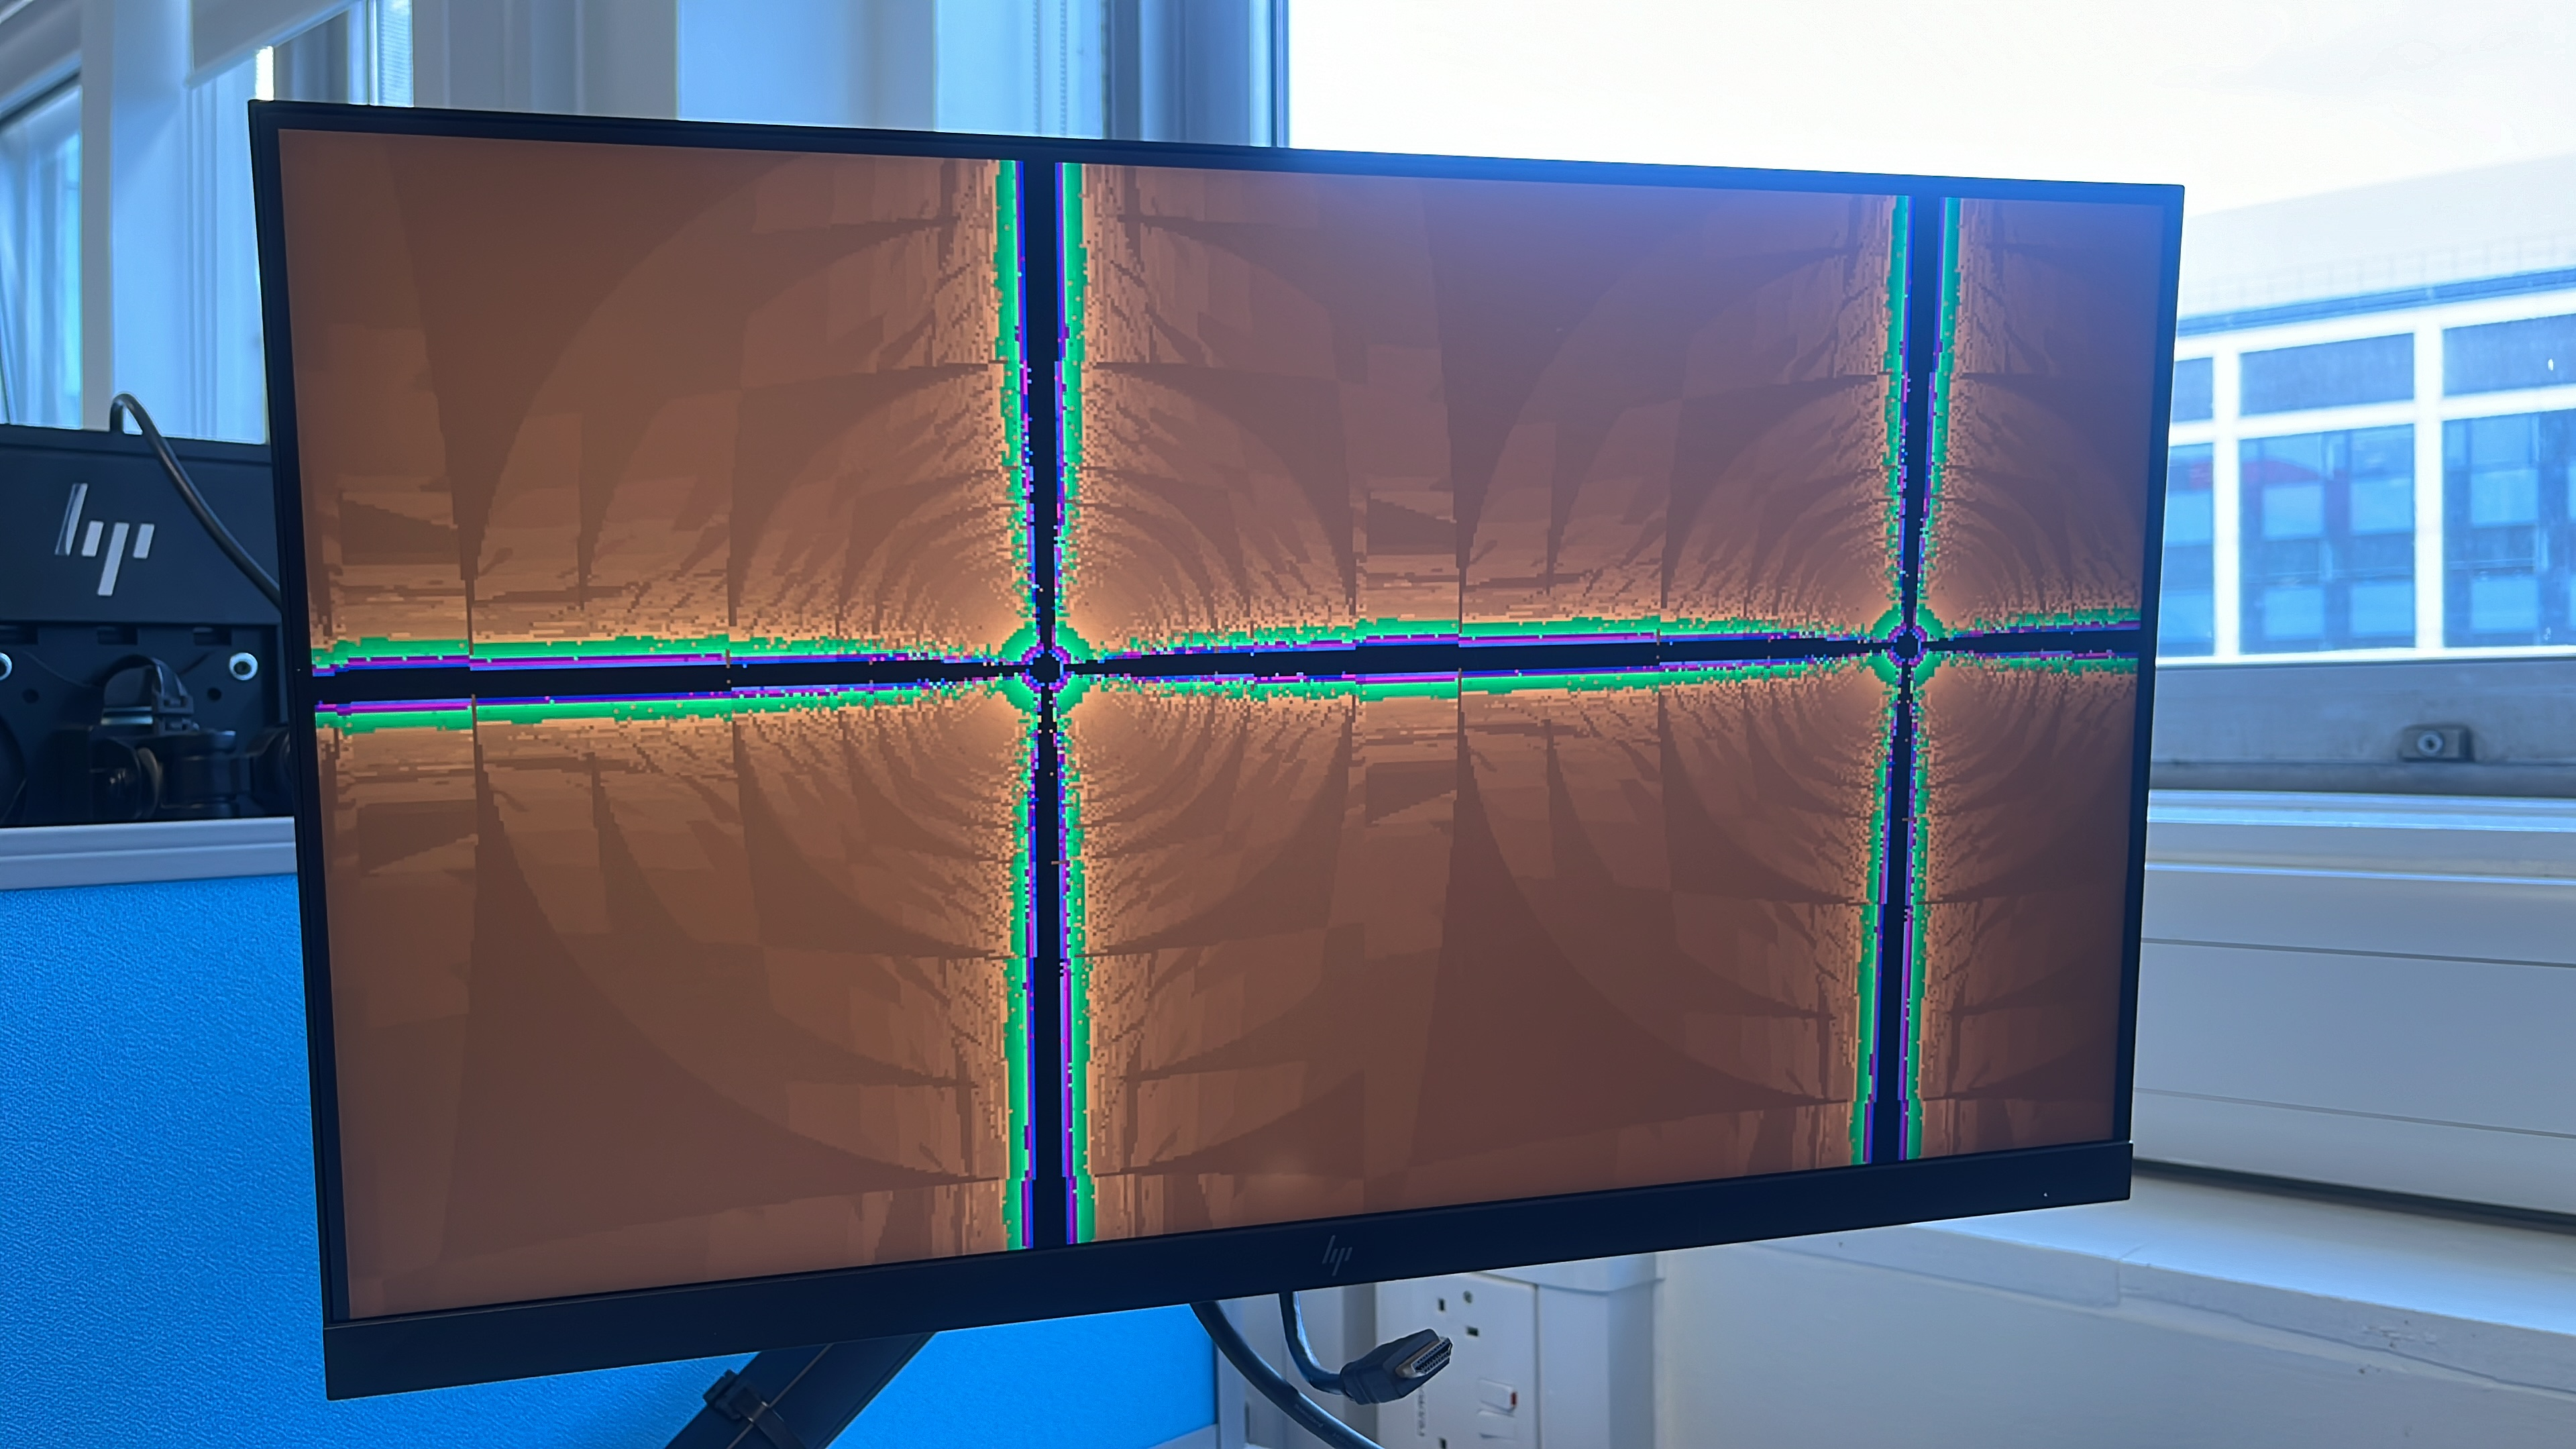
\includegraphics[width=\textwidth,height=0.28\textheight,keepaspectratio]{imgs/AppendixA/render_scaffold_debug_early.jpg}
    \caption{Early mandelbox debug render. Orange cross-hatch output; sync artefacts visible from uncalibrated VDMA buffer timing.}
\end{subfigure}\hfill
\begin{subfigure}[b]{0.48\textwidth}
    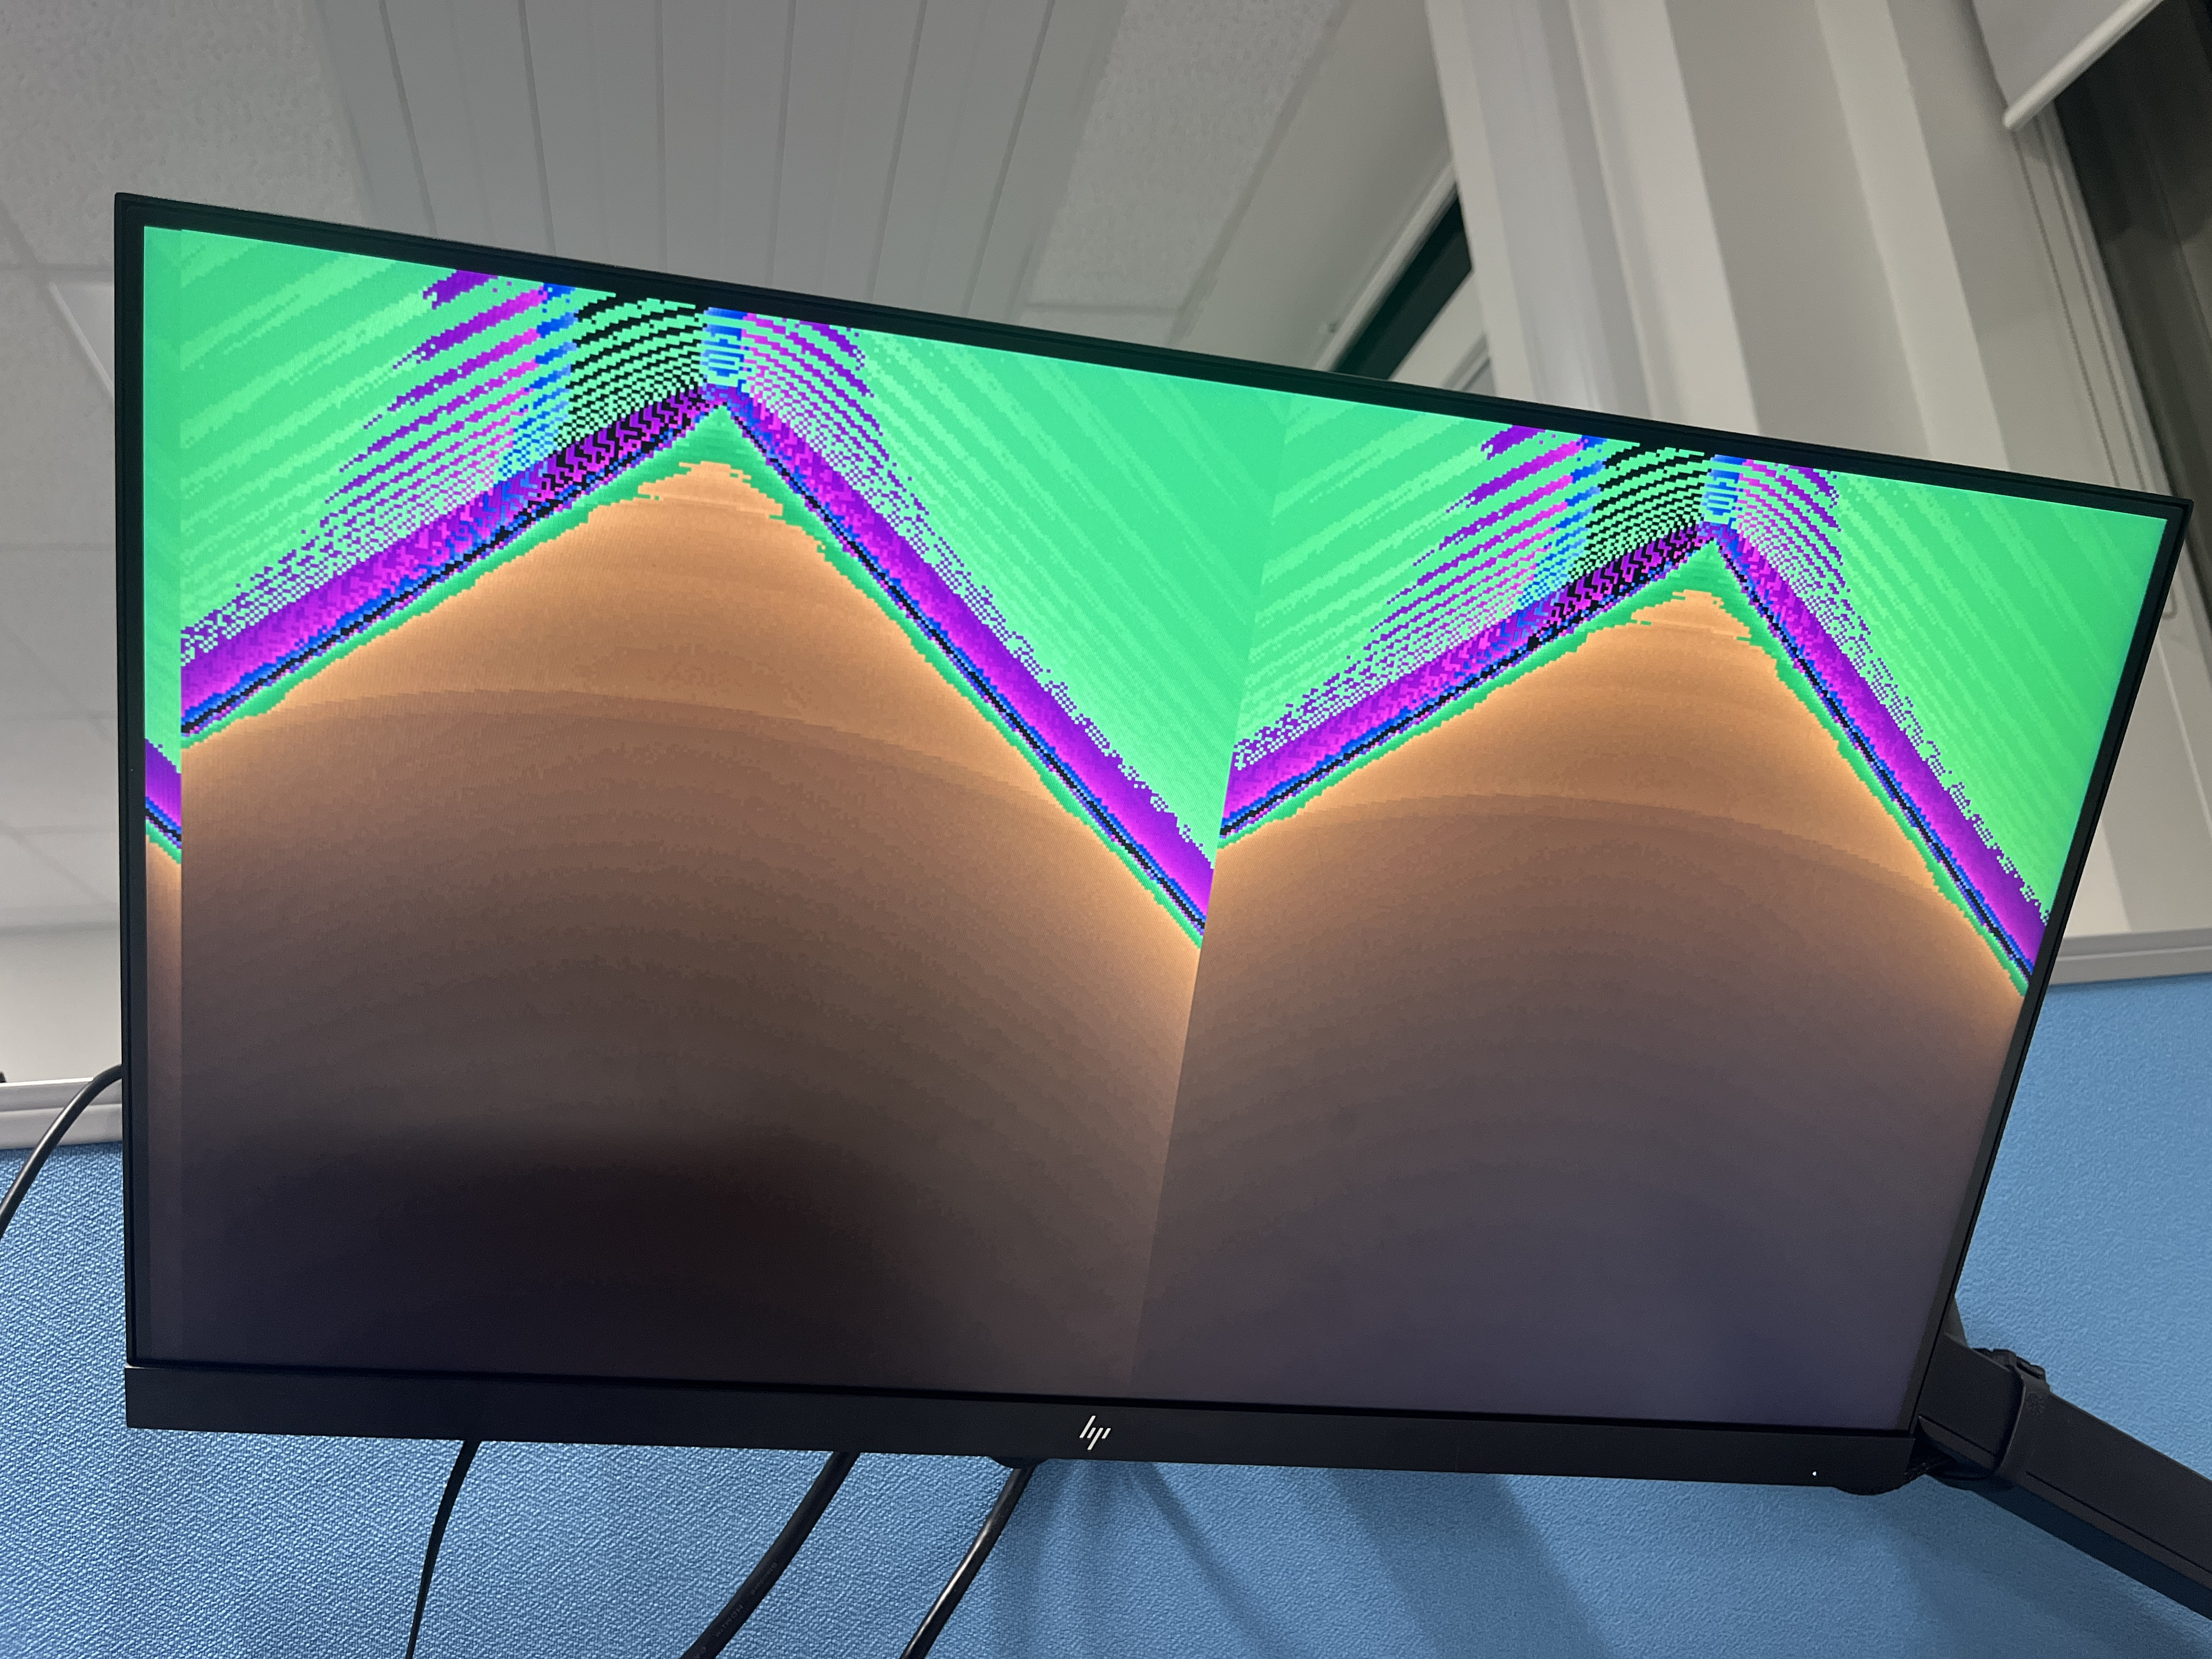
\includegraphics[width=\textwidth,height=0.28\textheight,keepaspectratio]{imgs/AppendixA/render_gyroid_early_stereo.jpg}
    \caption{Early cone, stereoscopic output. Wavy organic geometry with green--purple--orange iteration palette.}
\end{subfigure}

\vfill

\begin{subfigure}[b]{0.48\textwidth}
    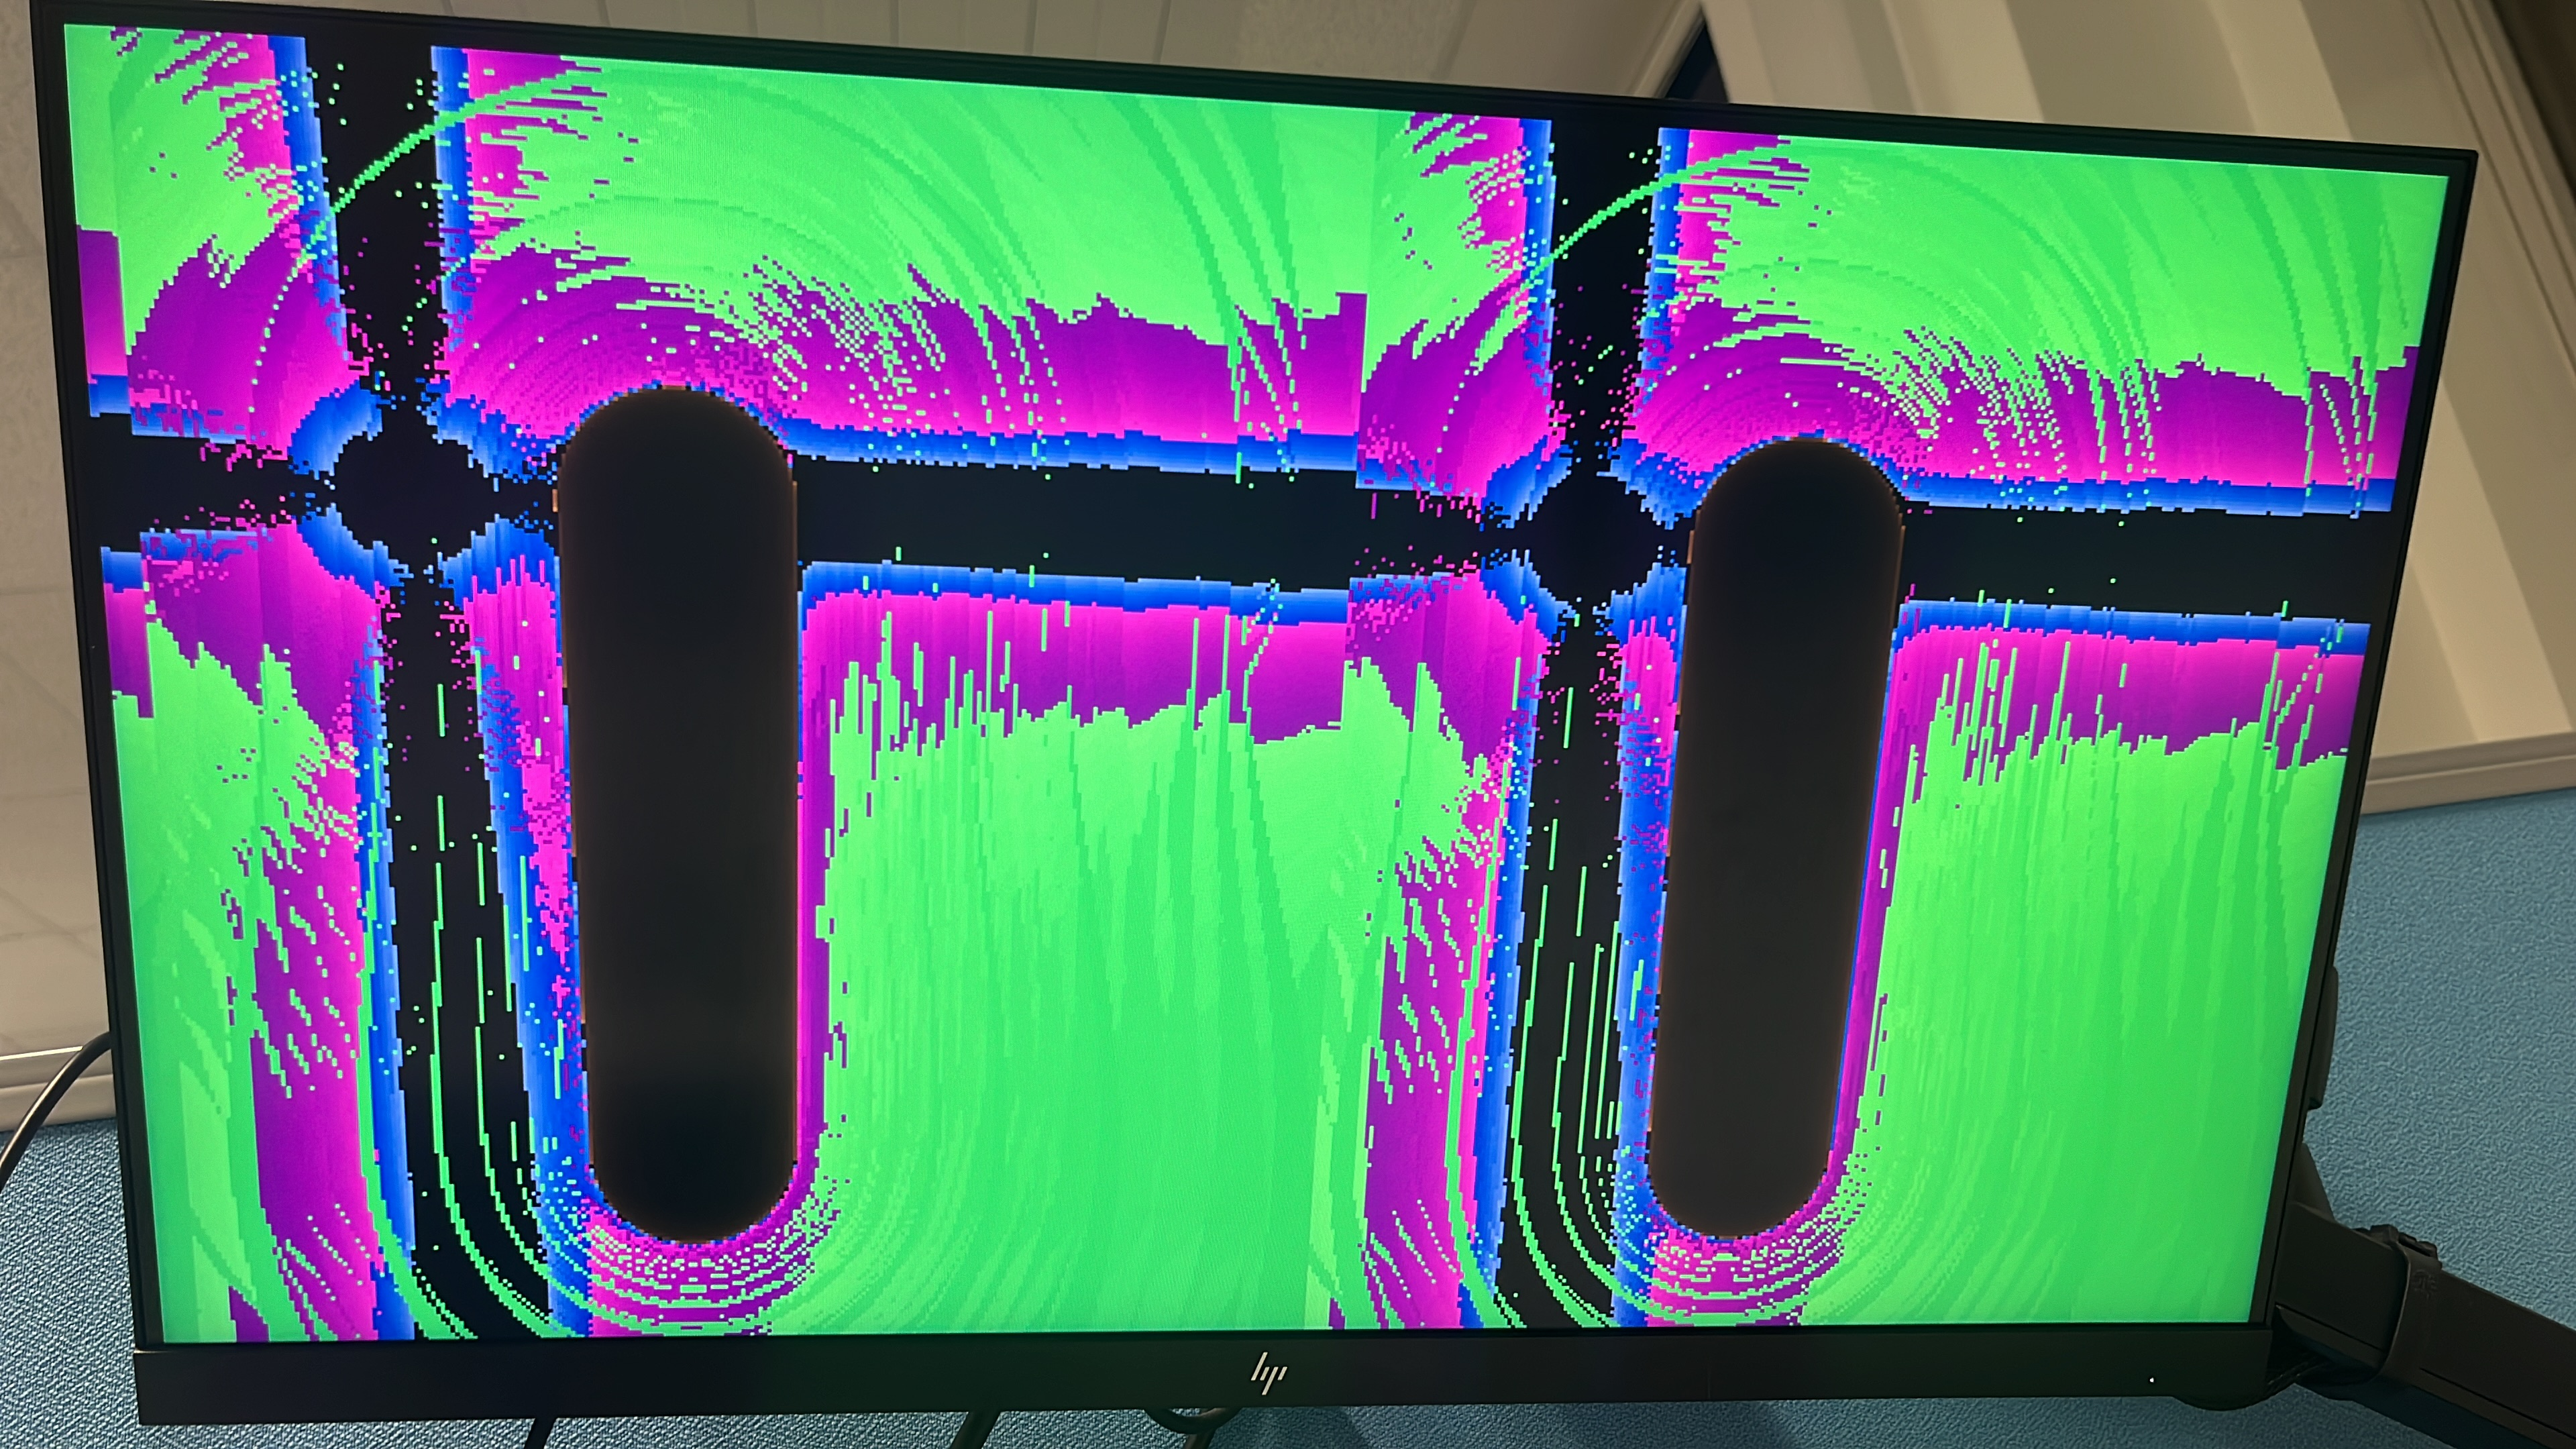
\includegraphics[width=\textwidth,height=0.28\textheight,keepaspectratio]{imgs/AppendixA/render_torus_stereo.jpg}
    \caption{Torus SDF in stereoscopic mode. Vivid green--purple colourmap; concave annular region visible at centre.}
\end{subfigure}\hfill
\begin{subfigure}[b]{0.48\textwidth}
    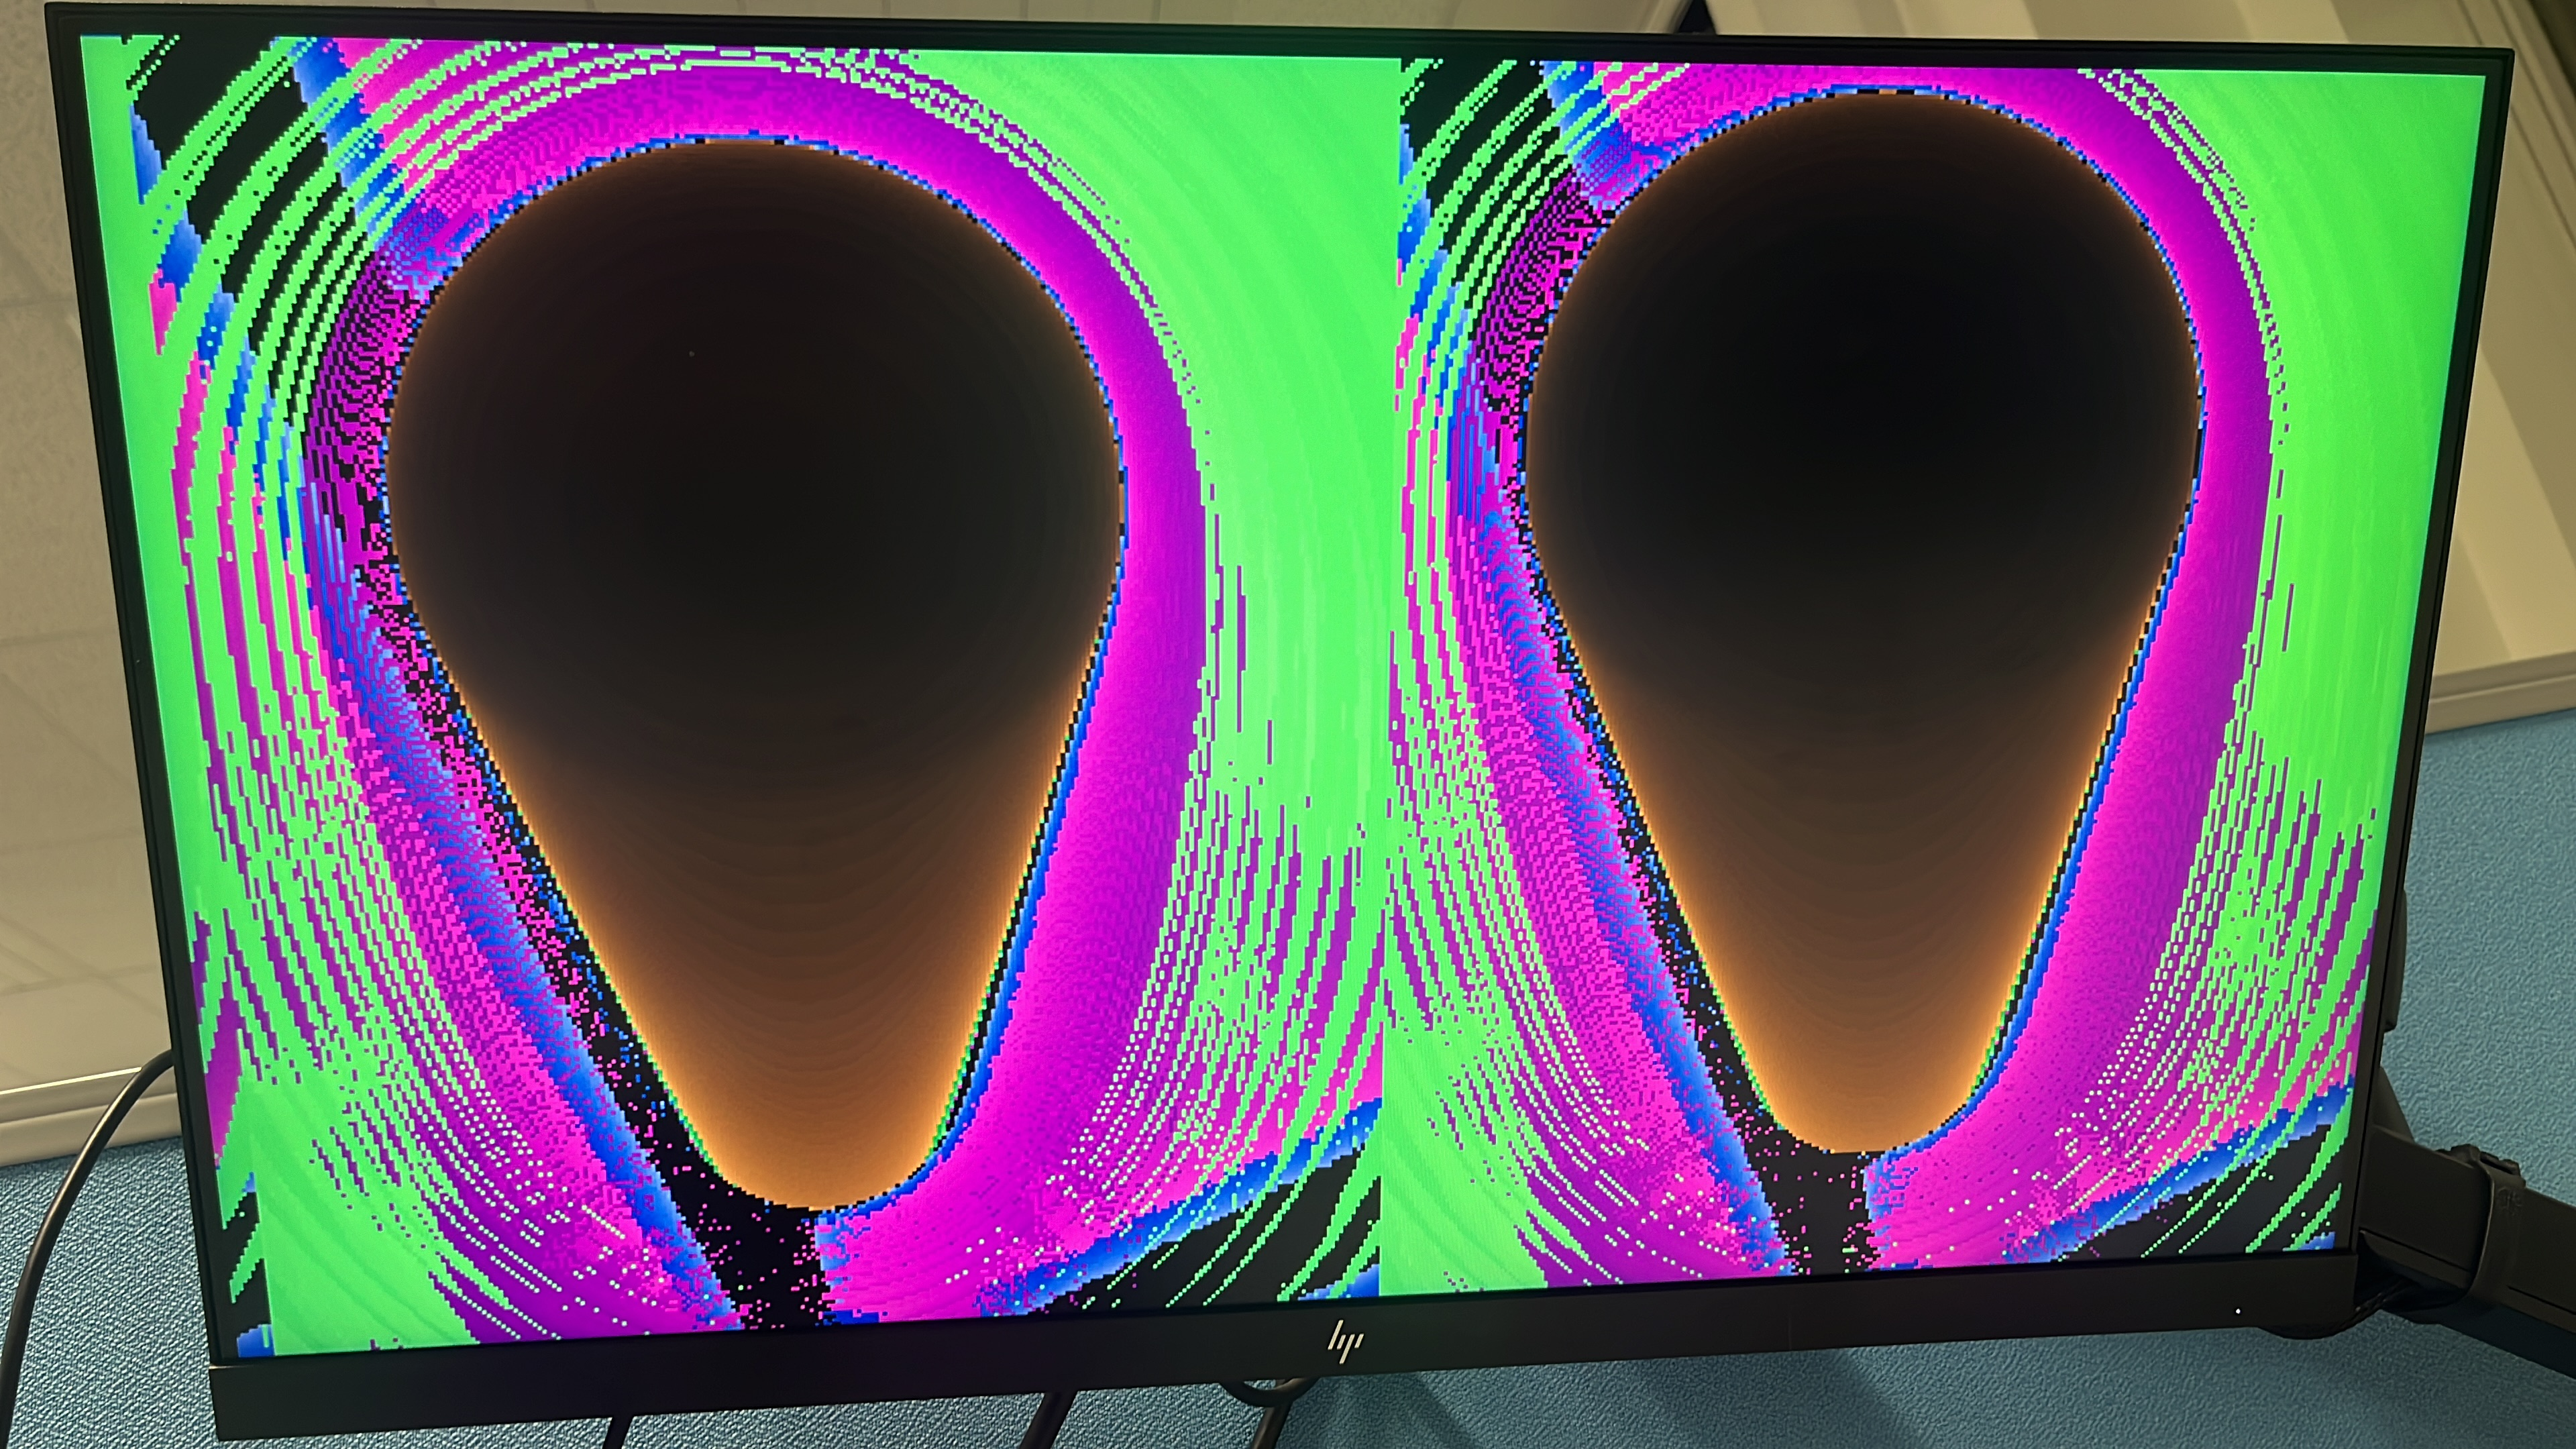
\includegraphics[width=\textwidth,height=0.28\textheight,keepaspectratio]{imgs/AppendixA/render_hyperboloid_stereo.jpg}
    \caption{Capsule SDF, single-sheet geometry. Large teardrop profile against green--purple background.}
\end{subfigure}

\vfill

\begin{subfigure}[b]{0.48\textwidth}
    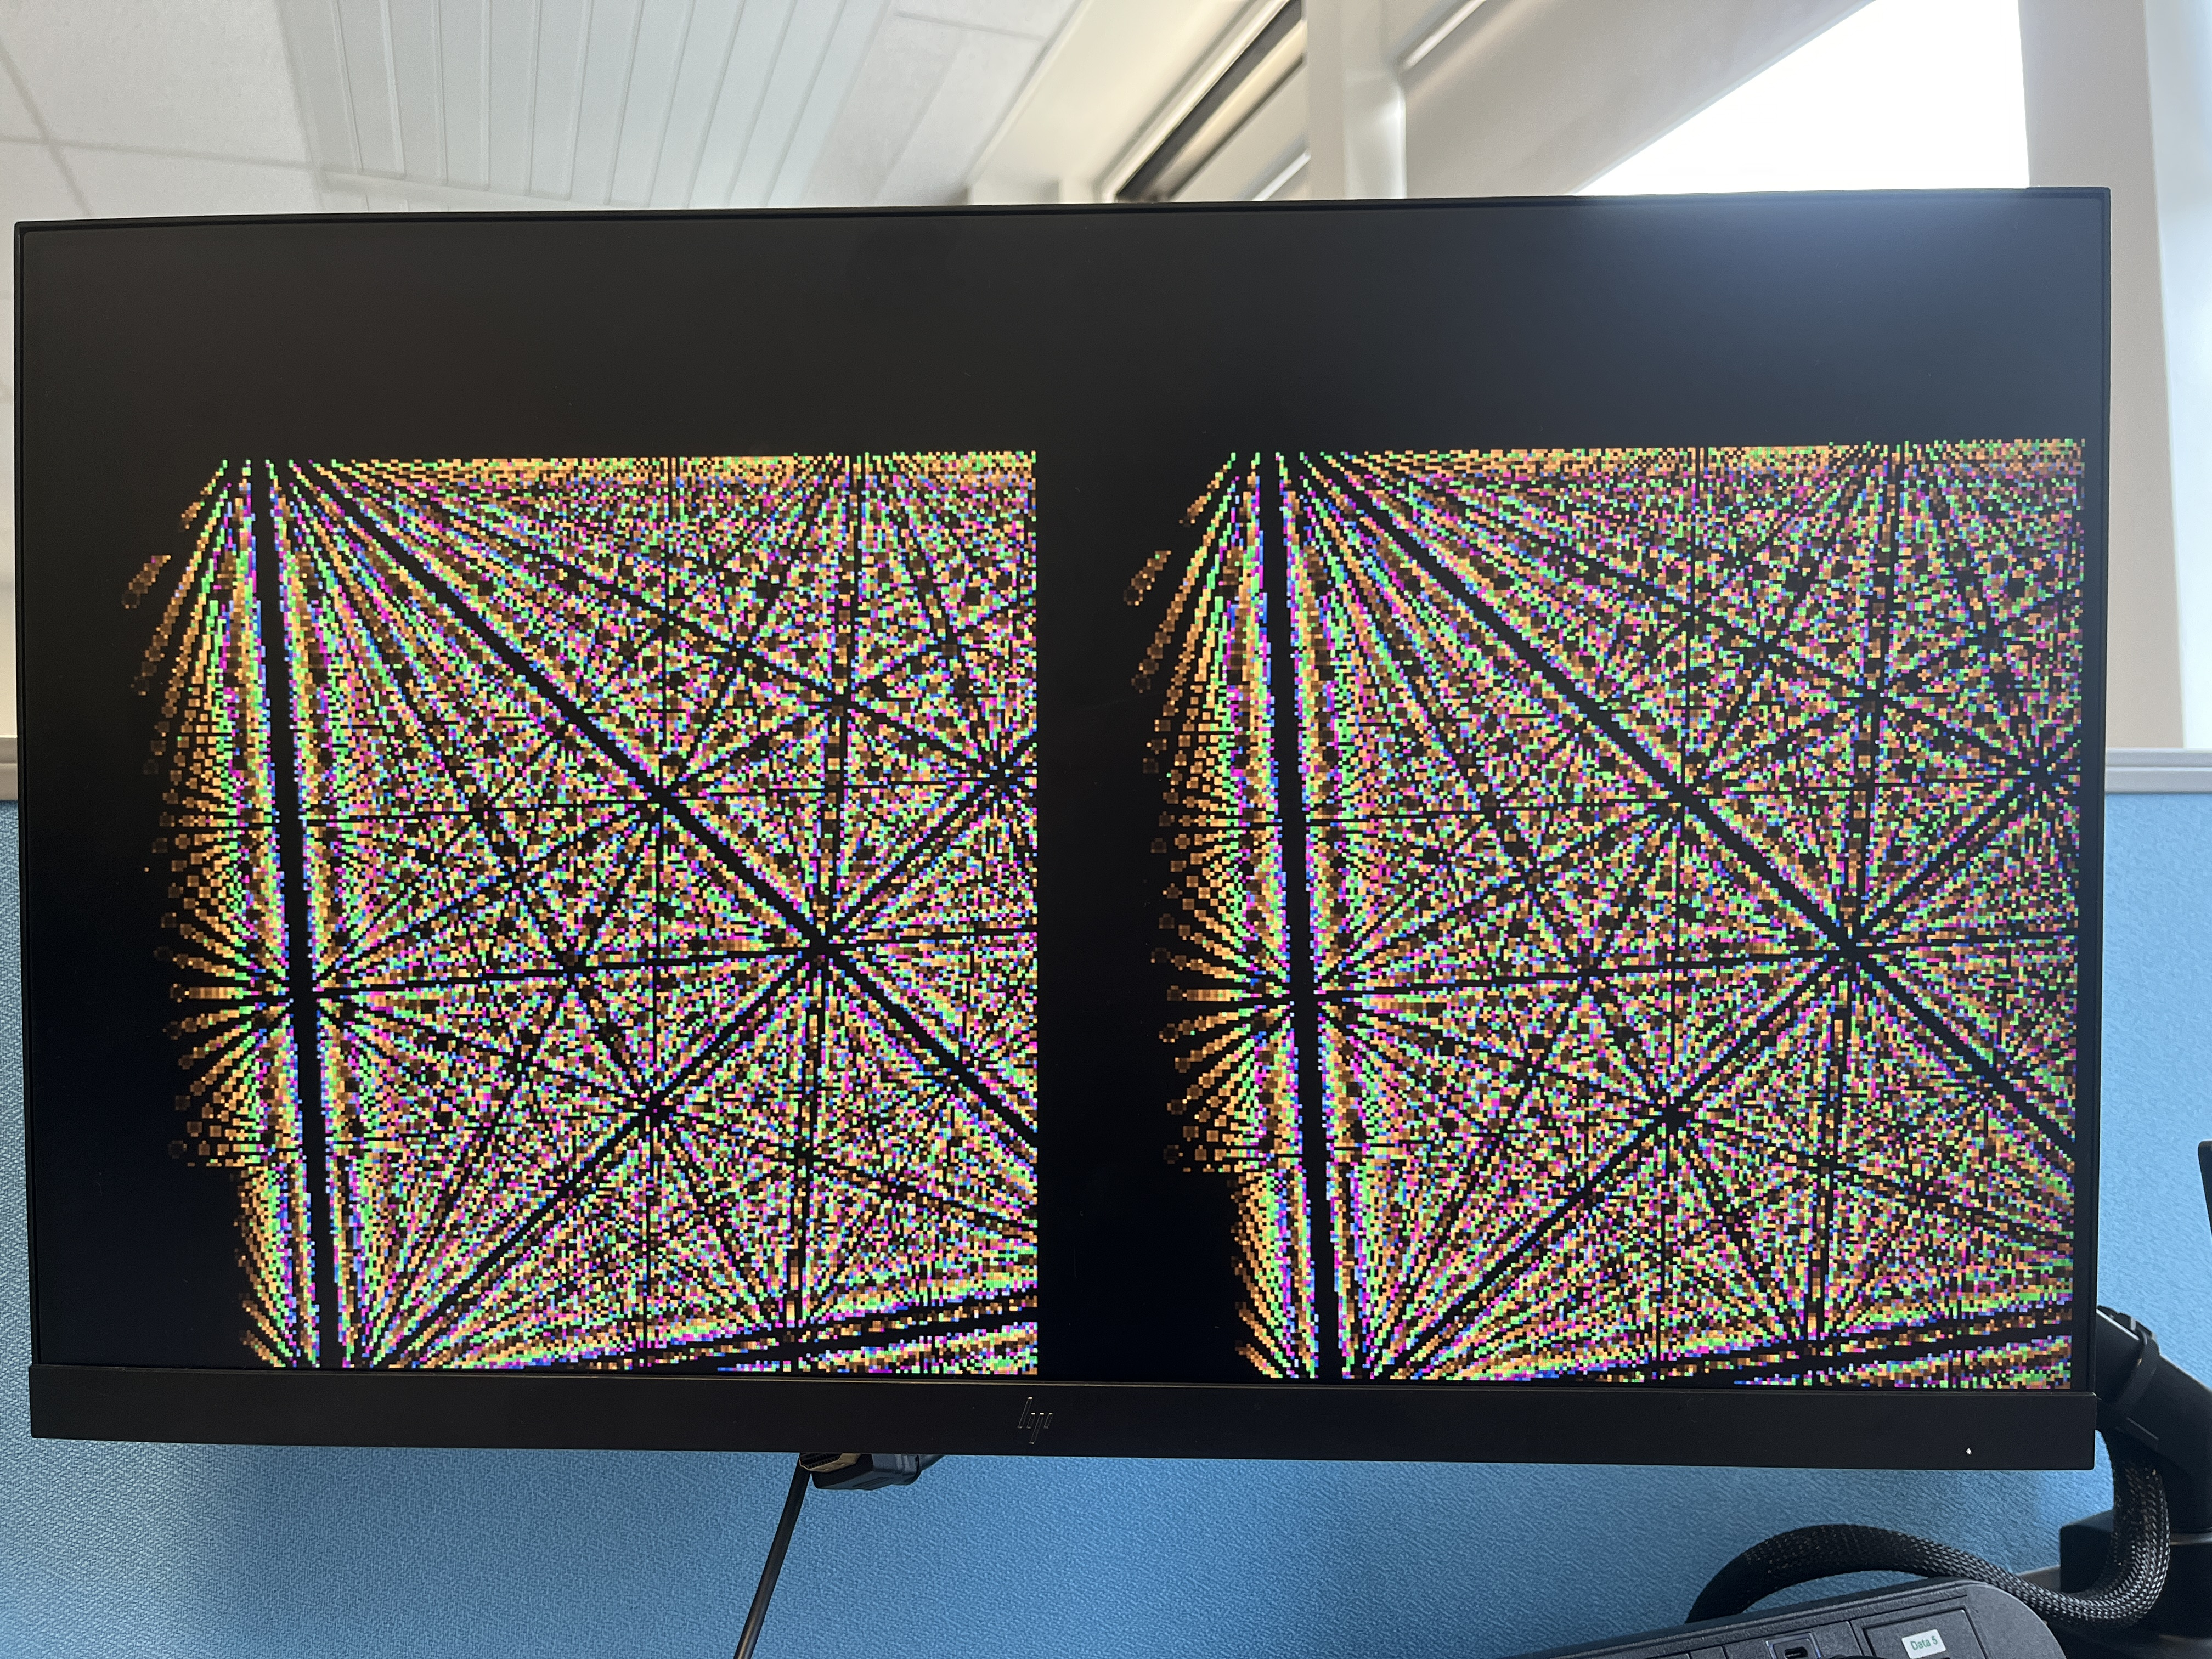
\includegraphics[width=\textwidth,height=0.28\textheight,keepaspectratio]{imgs/AppendixA/render_scaffold_lattice_stereo.jpg}
    \caption{Sphere box-frame lattice on black background. Diamond grid from space repetition, \texttt{cell\_size} $= 2$.}
\end{subfigure}\hfill
\begin{subfigure}[b]{0.48\textwidth}
    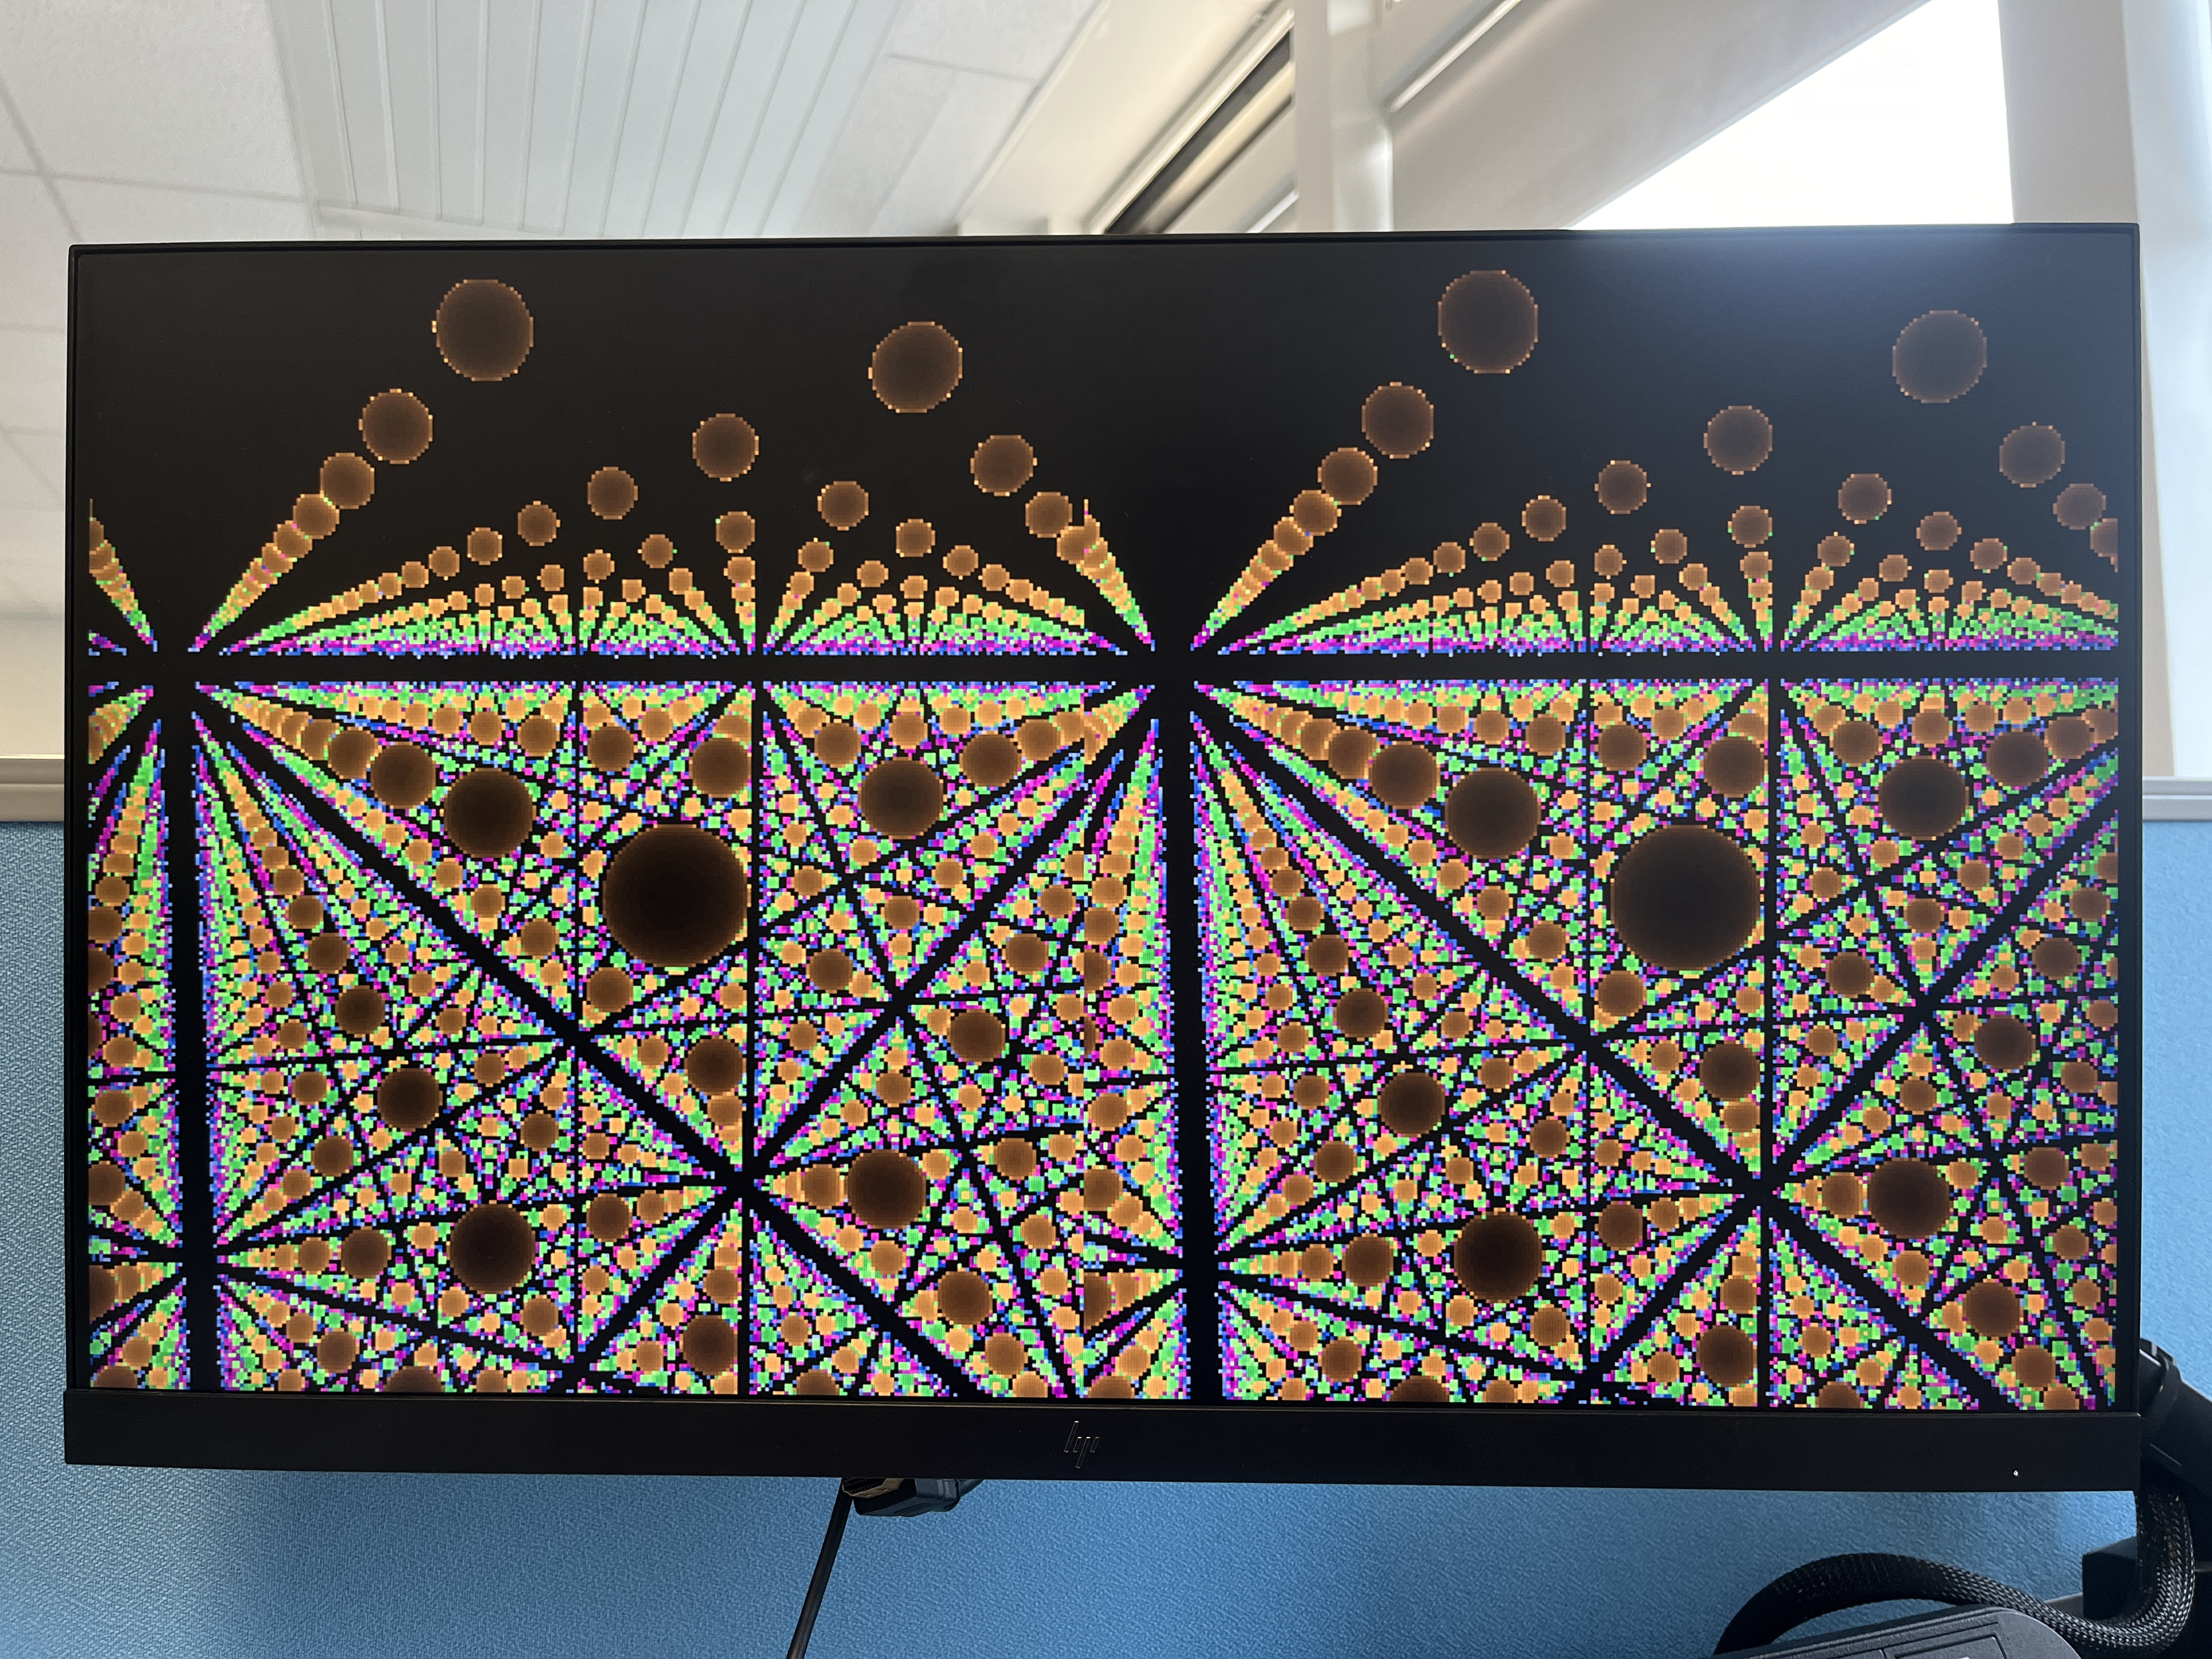
\includegraphics[width=\textwidth,height=0.28\textheight,keepaspectratio]{imgs/AppendixA/render_gyroid_spheres_stereo.jpg}
    \caption{Sphere with space-repeated sphere array. Infinite lattice viewed from close range, \texttt{cell\_size} $= 10$.}
\end{subfigure}
\caption{Stereoscopic render gallery I: early hardware output on external monitor.}
\end{figure}

\clearpage

% ----------------------------------------------------------------
%  Page 2 — Mandelbox variants + gyroid spheres variant + headset
% ----------------------------------------------------------------
\begin{figure}[H]
\vspace*{-0.5cm}
\centering
\begin{subfigure}[b]{0.48\textwidth}
    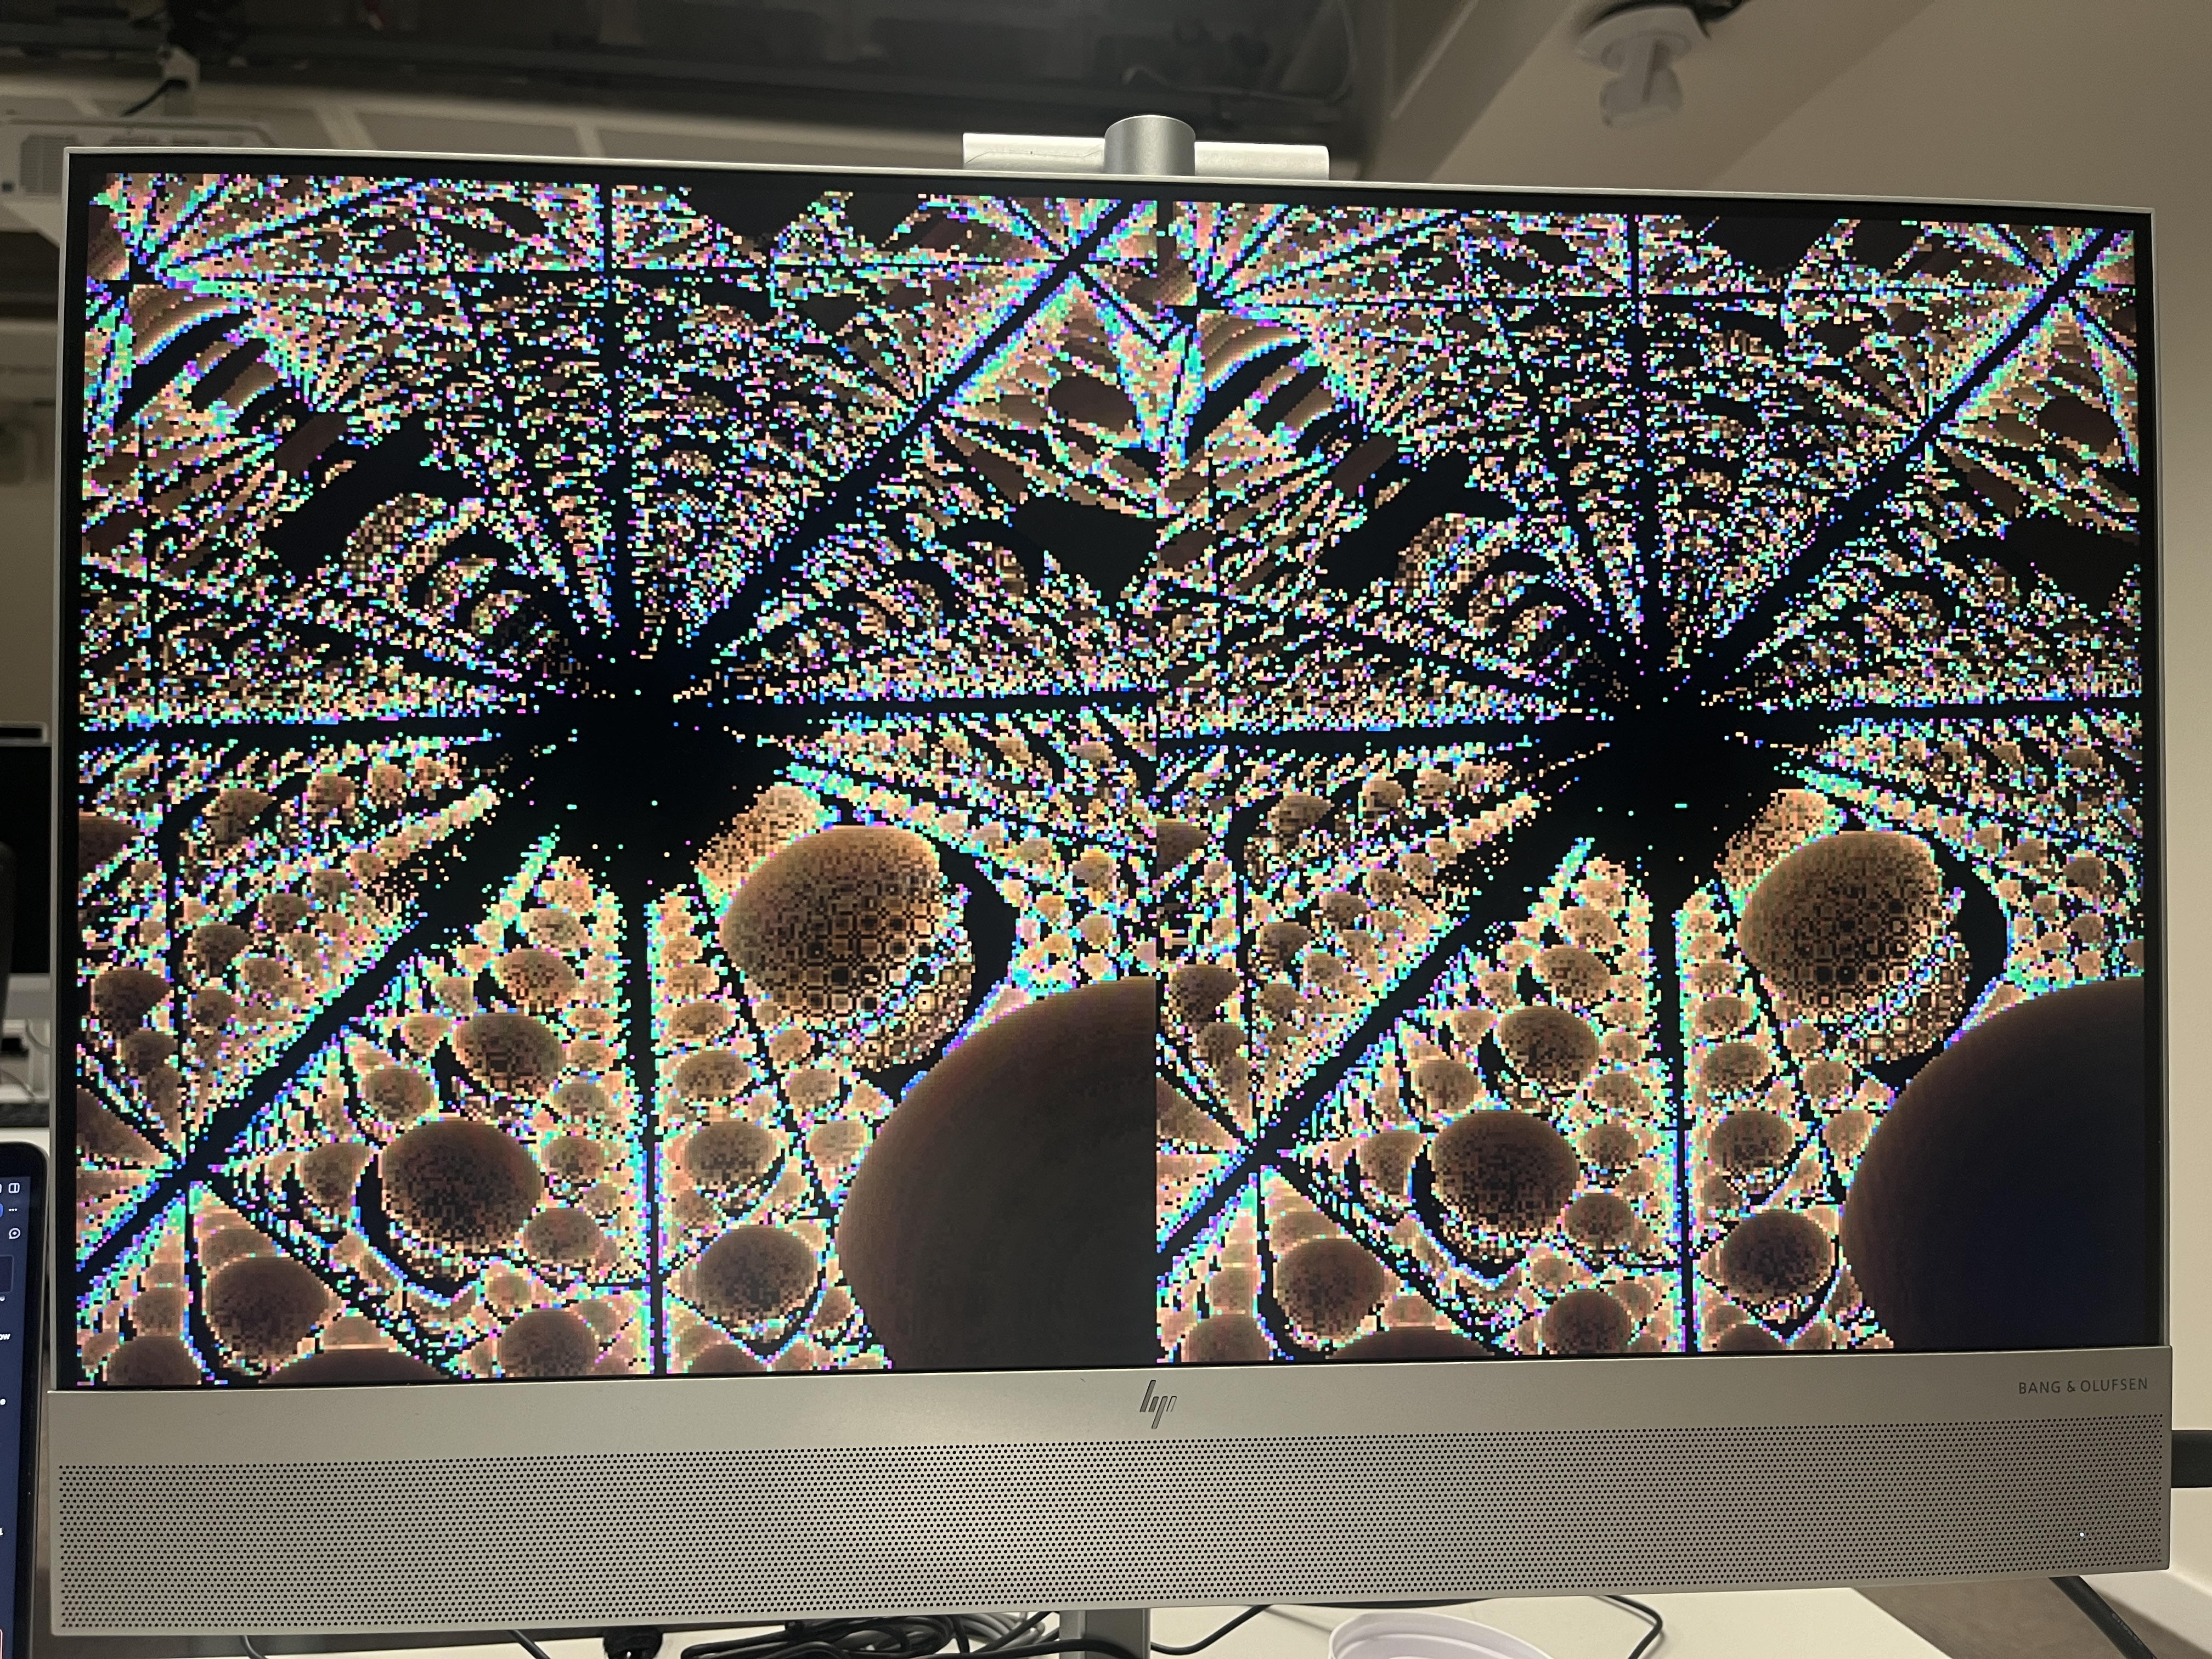
\includegraphics[width=\textwidth,height=0.28\textheight,keepaspectratio]{imgs/AppendixA/render_mandelbox_closeup_stereo.jpg}
    \caption{Sphere boundary close-up. Spiky self-similar structures at the exterior box-fold boundary due to approximations in NR}
\end{subfigure}\hfill
\begin{subfigure}[b]{0.48\textwidth}
    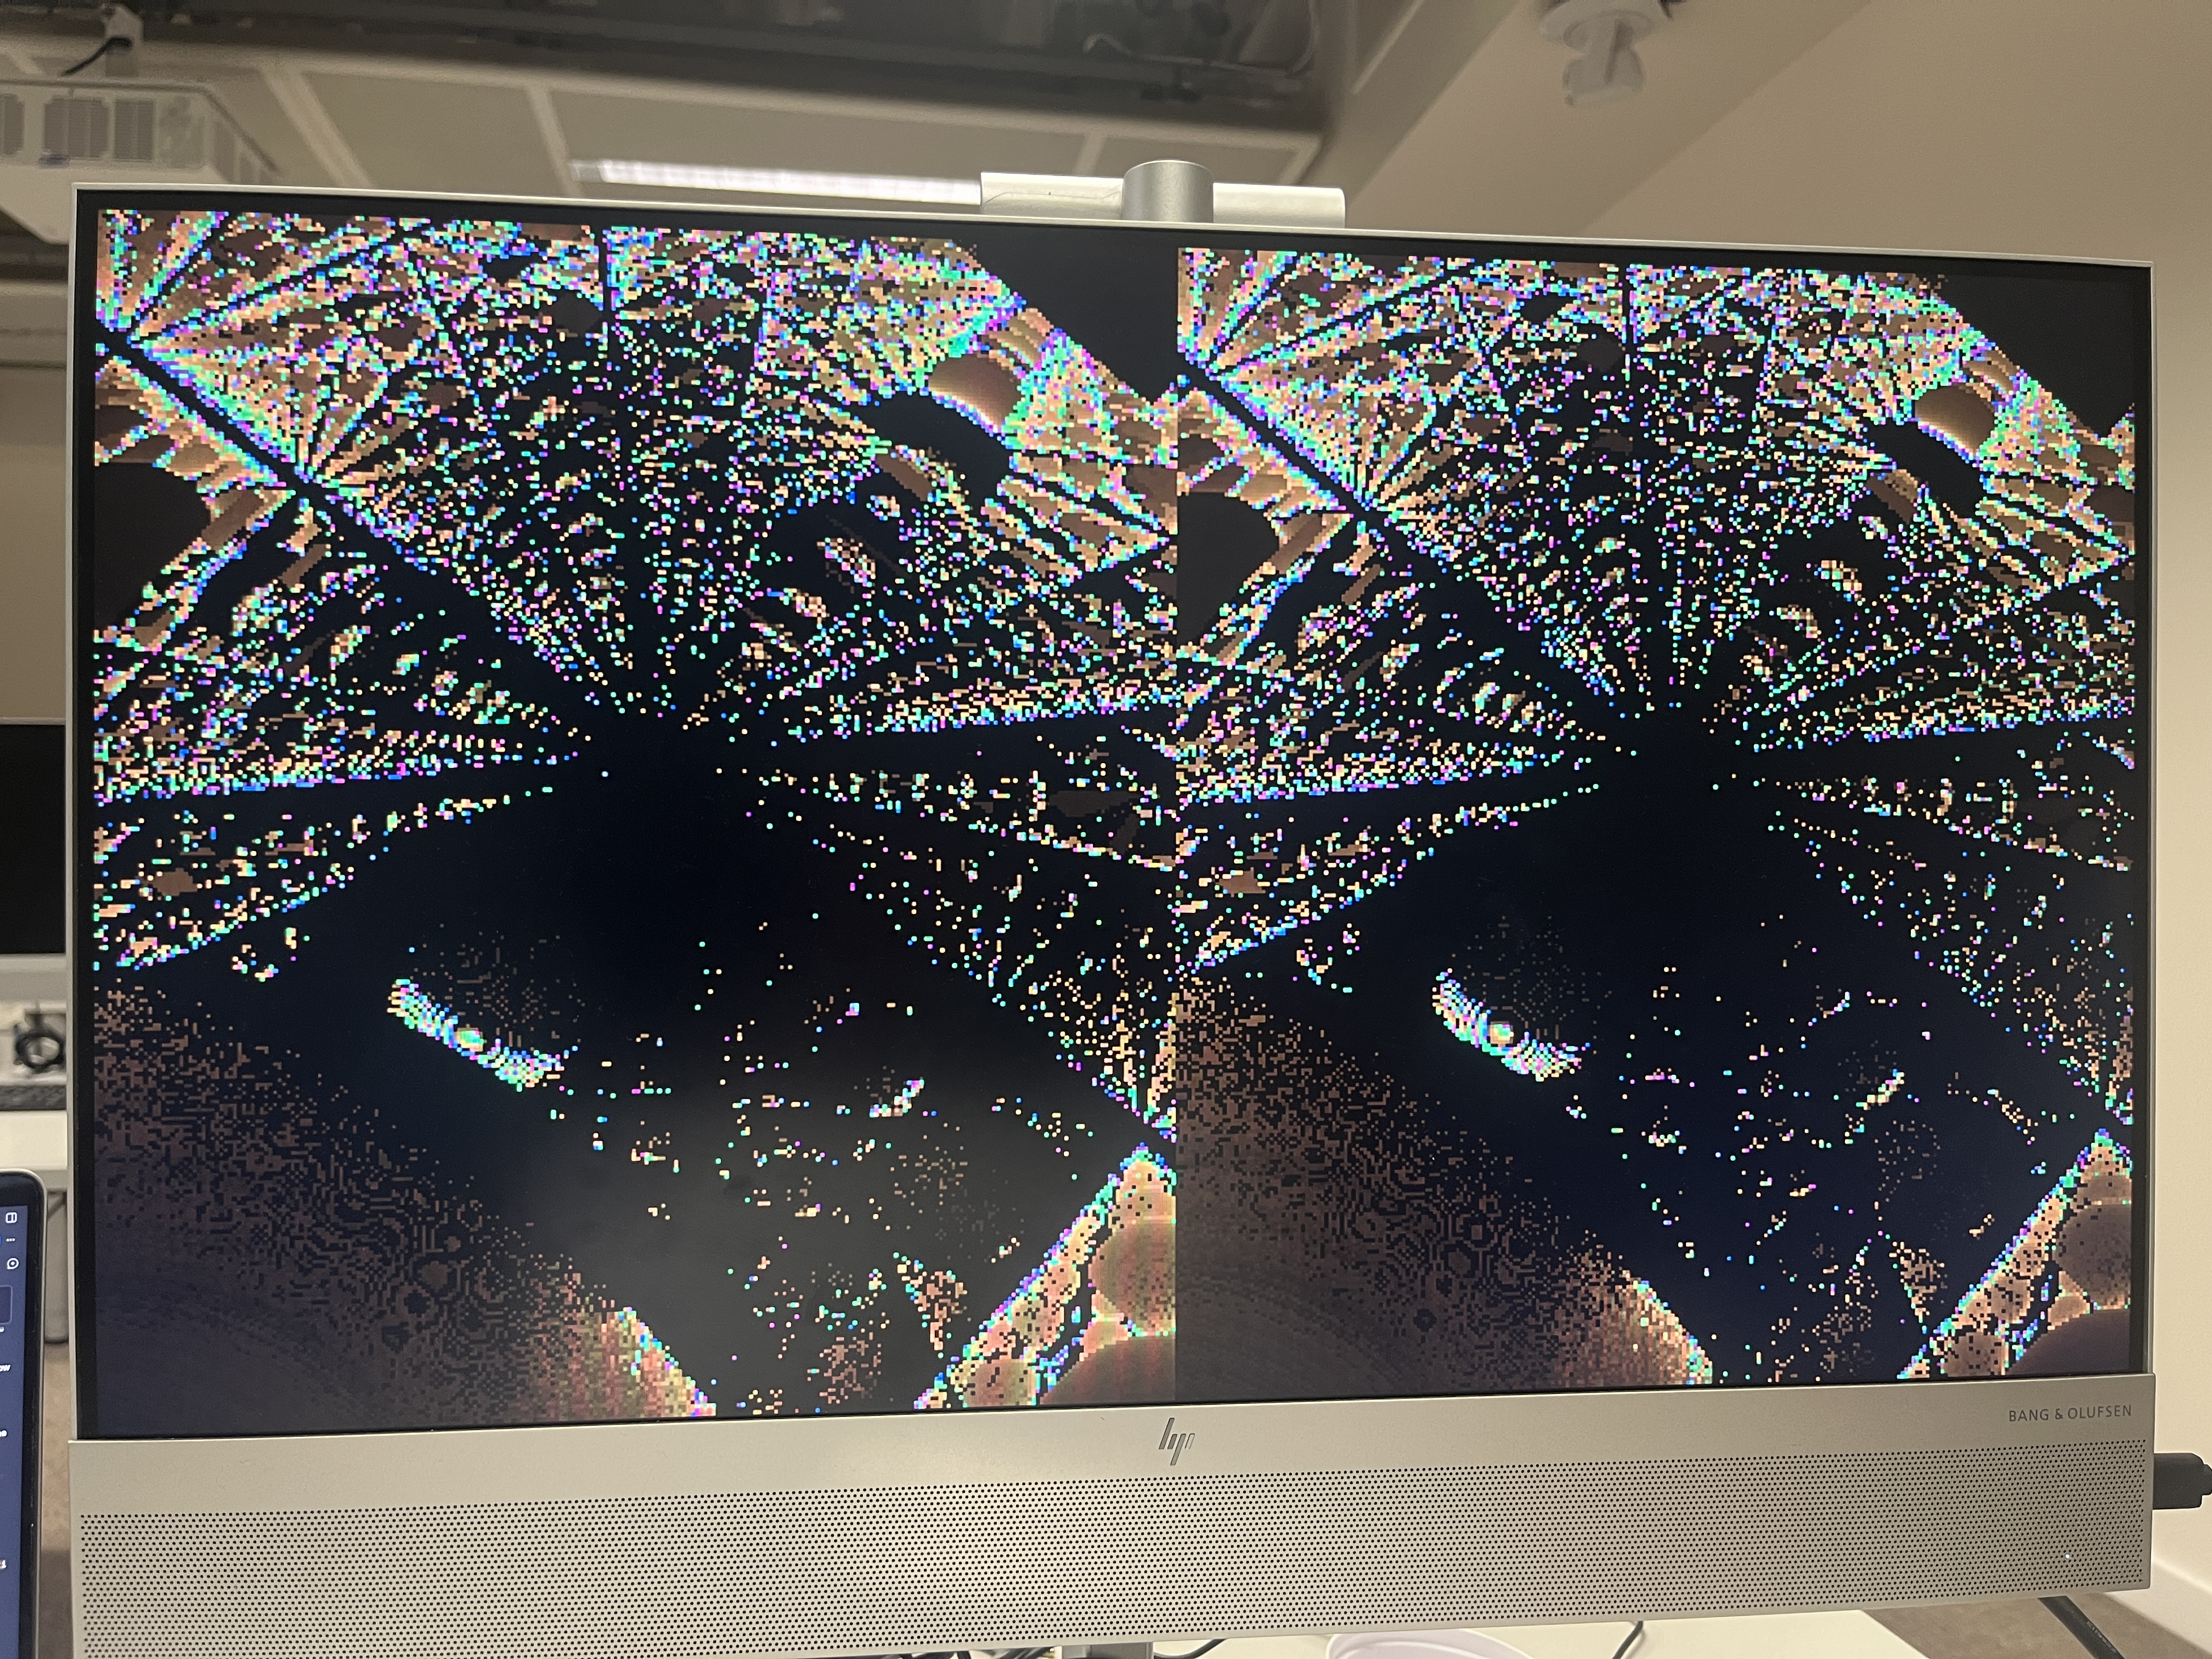
\includegraphics[width=\textwidth,height=0.28\textheight,keepaspectratio]{imgs/AppendixA/render_mandelbox_interior_stereo.jpg}
    \caption{NR approximations acculumations.}
\end{subfigure}

\vfill

\begin{subfigure}[b]{0.48\textwidth}
    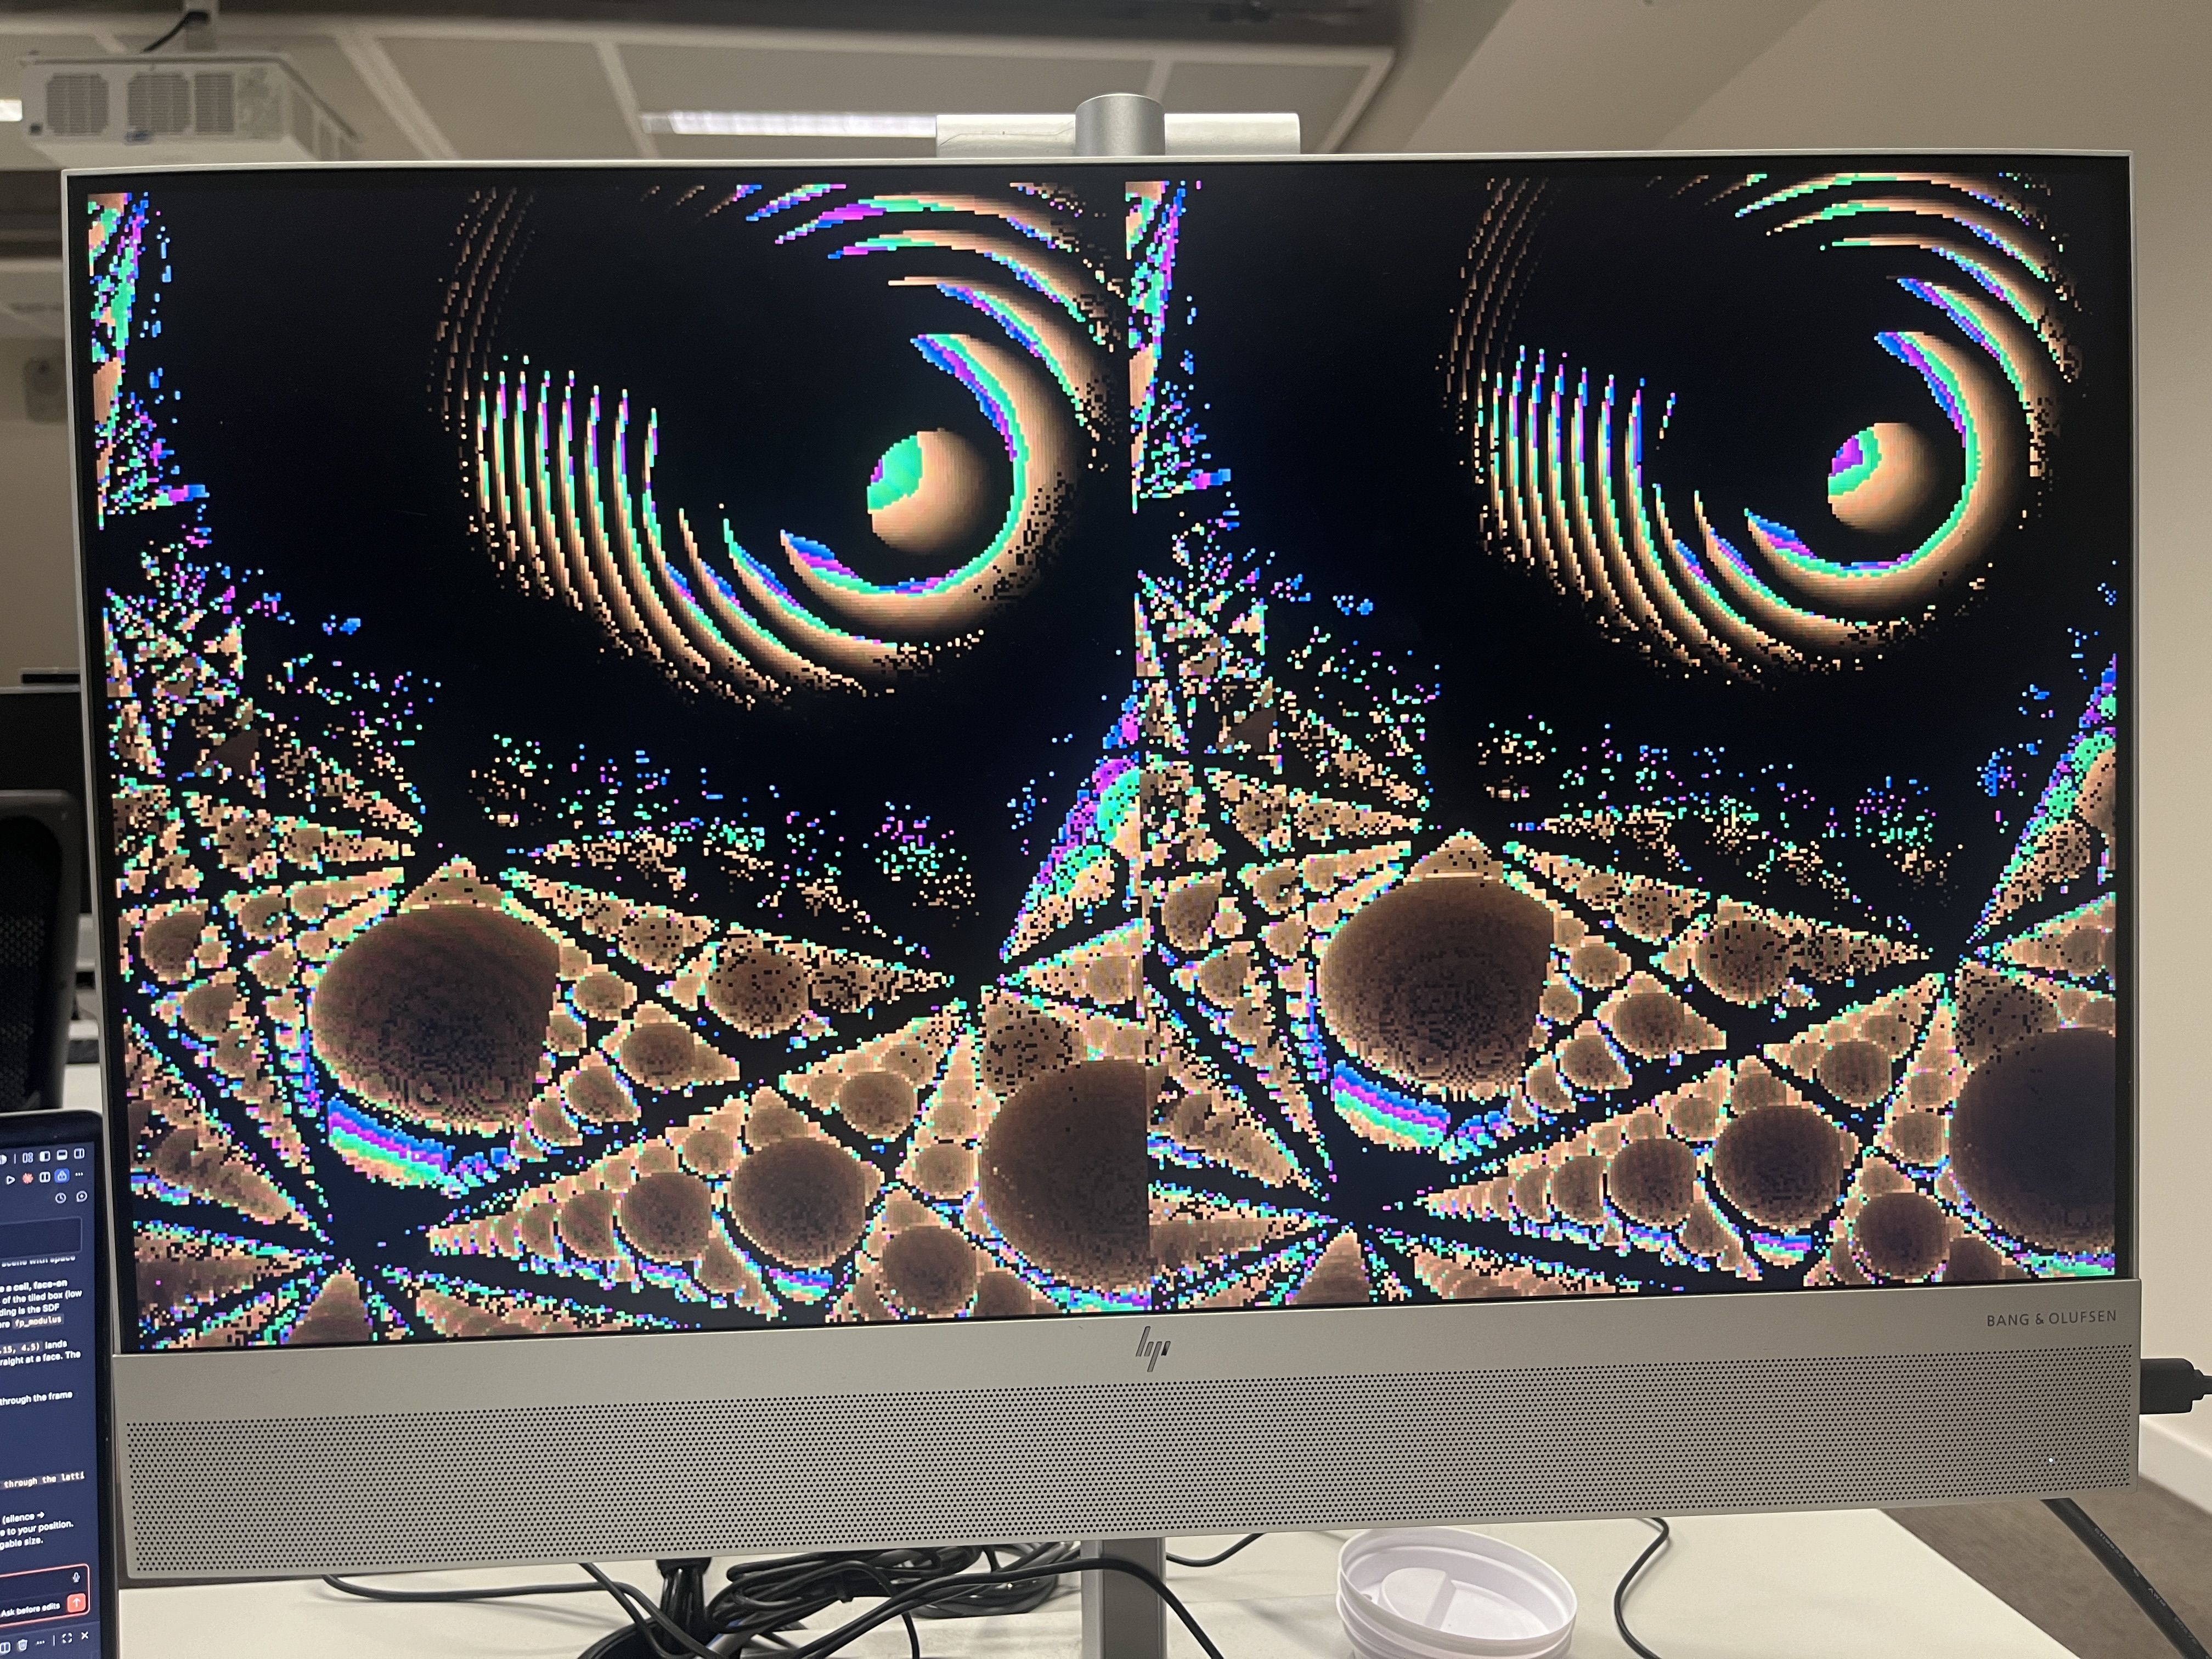
\includegraphics[width=\textwidth,height=0.28\textheight,keepaspectratio]{imgs/AppendixA/render_mandelbox_spiral_stereo.jpg}
    \caption{NR approximations acculumations.}
\end{subfigure}\hfill
\begin{subfigure}[b]{0.48\textwidth}
    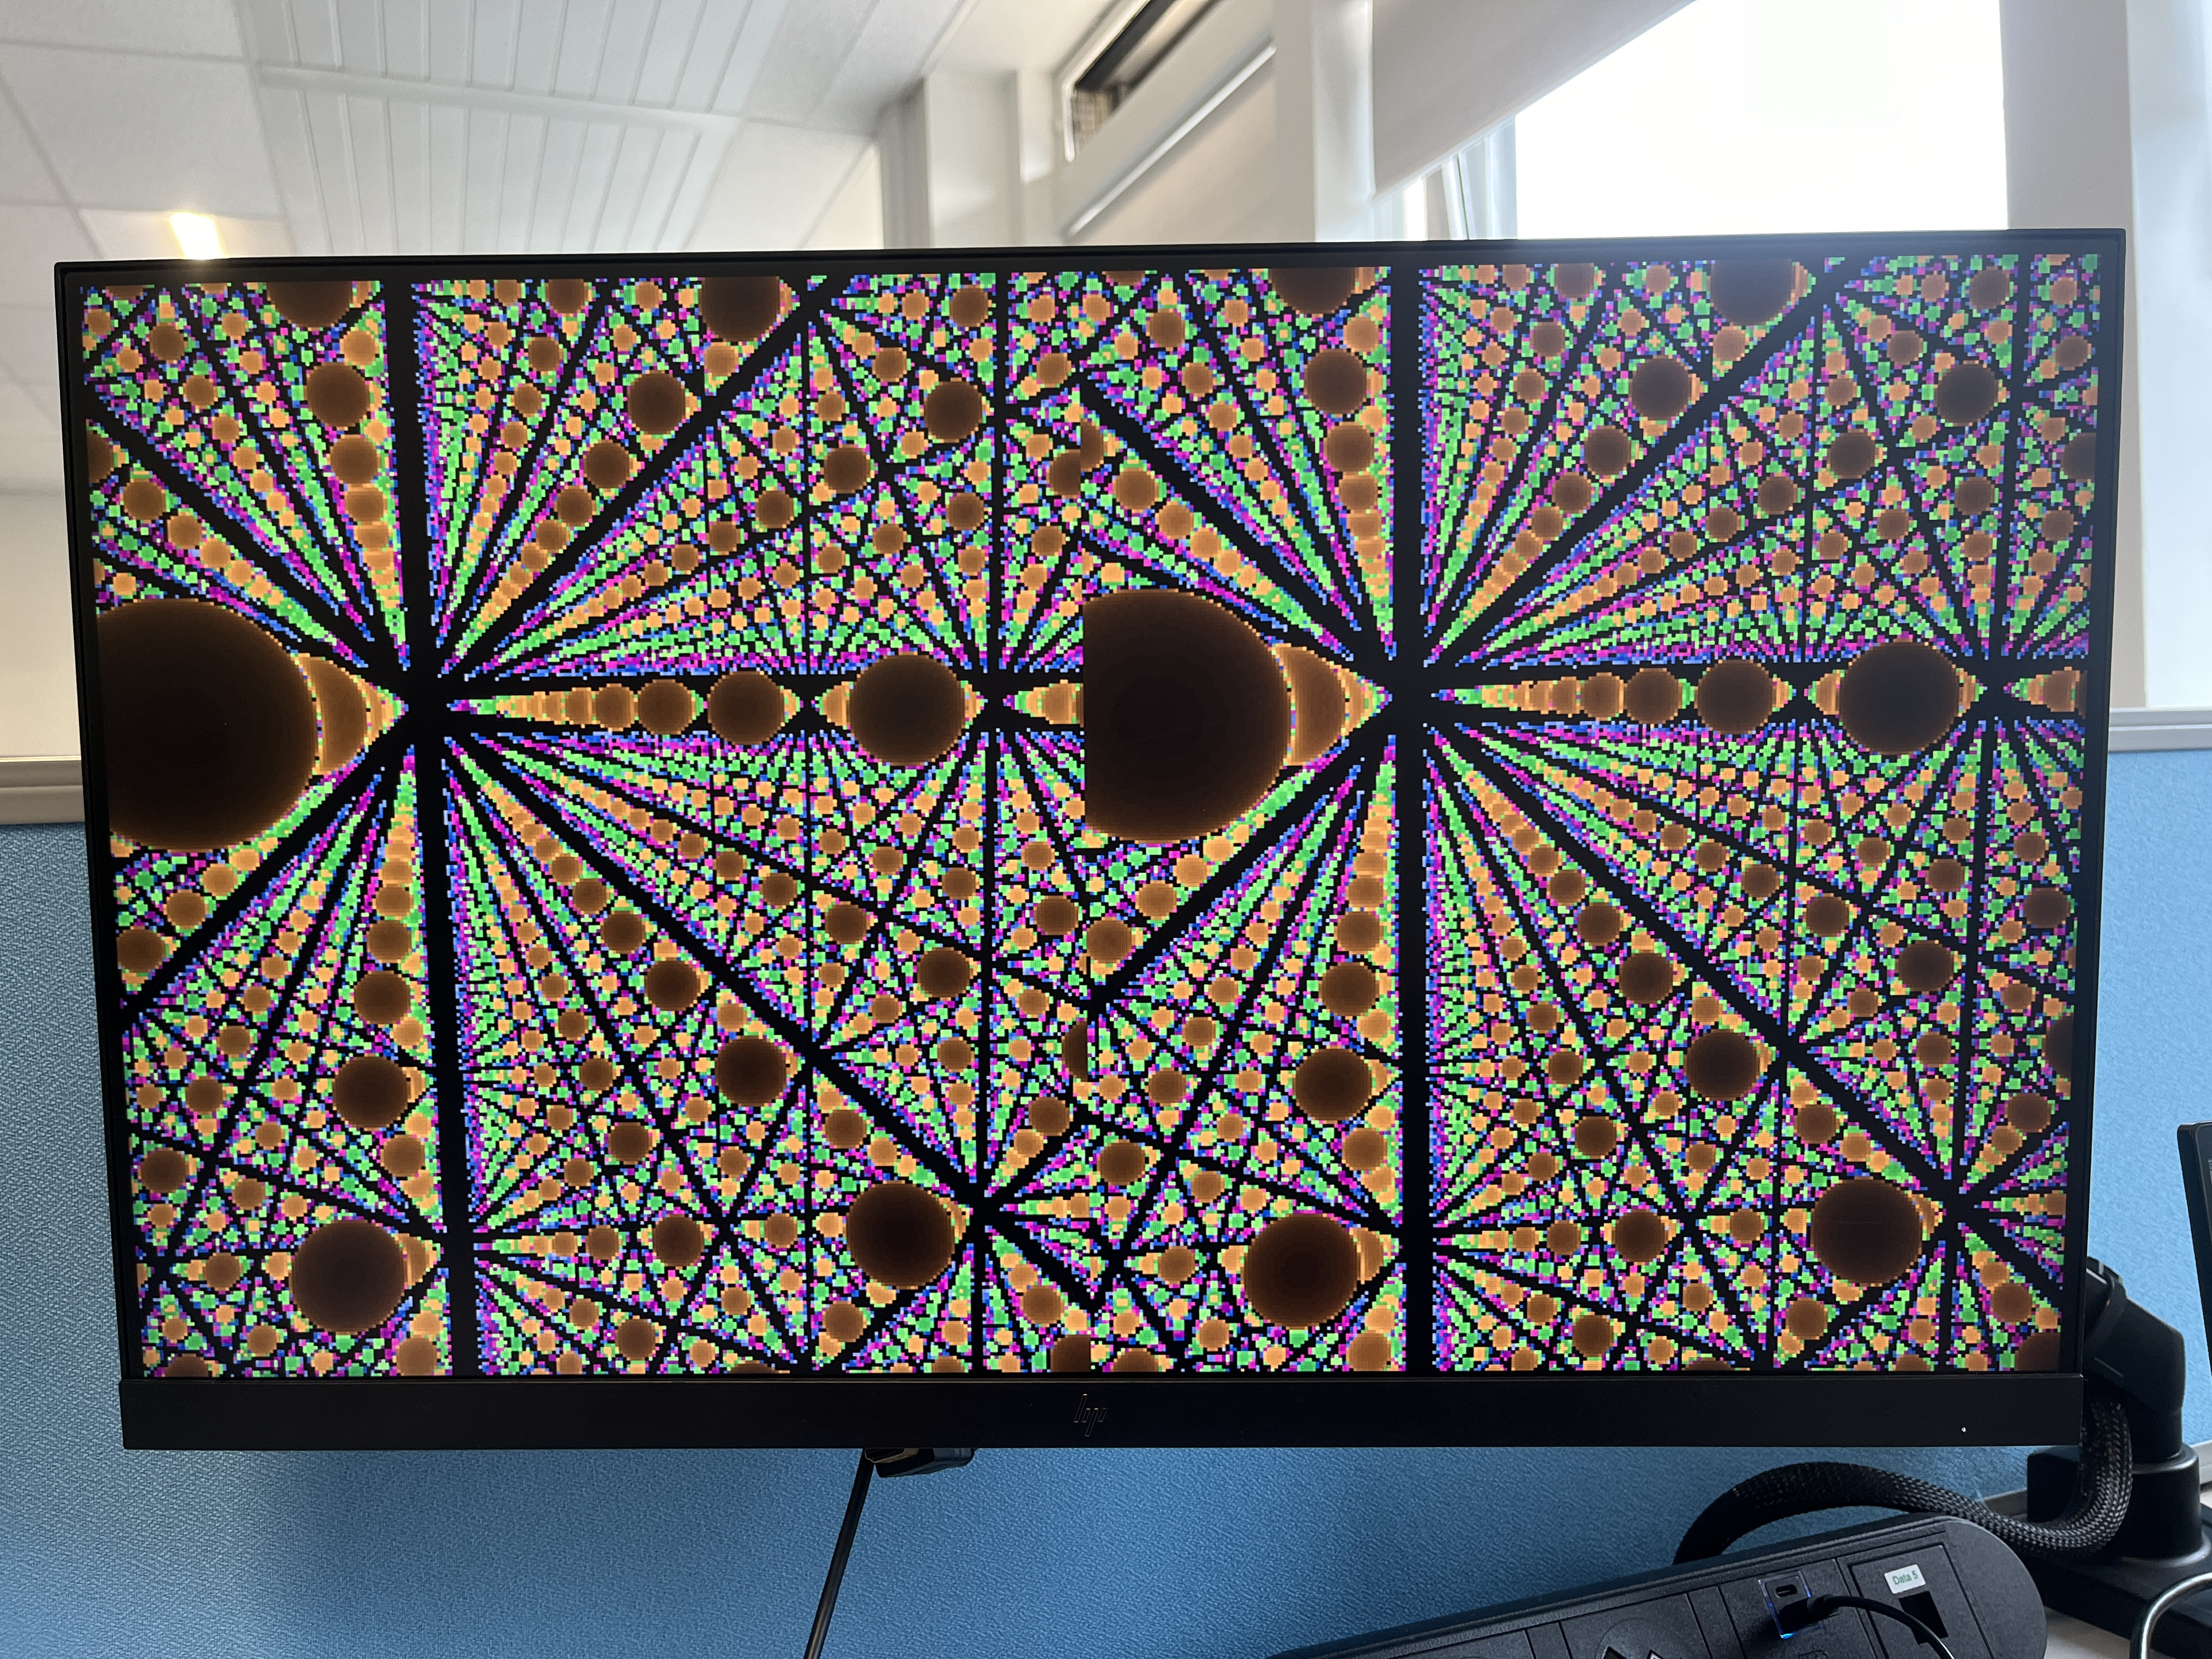
\includegraphics[width=\textwidth,height=0.28\textheight,keepaspectratio]{imgs/AppendixA/render_mandelbox_lattice_stereo.jpg}
    \caption{Infinite spheres, space-repeated with \texttt{cell\_size} $= 2$.}
\end{subfigure}

\vfill

\begin{subfigure}[b]{0.48\textwidth}
    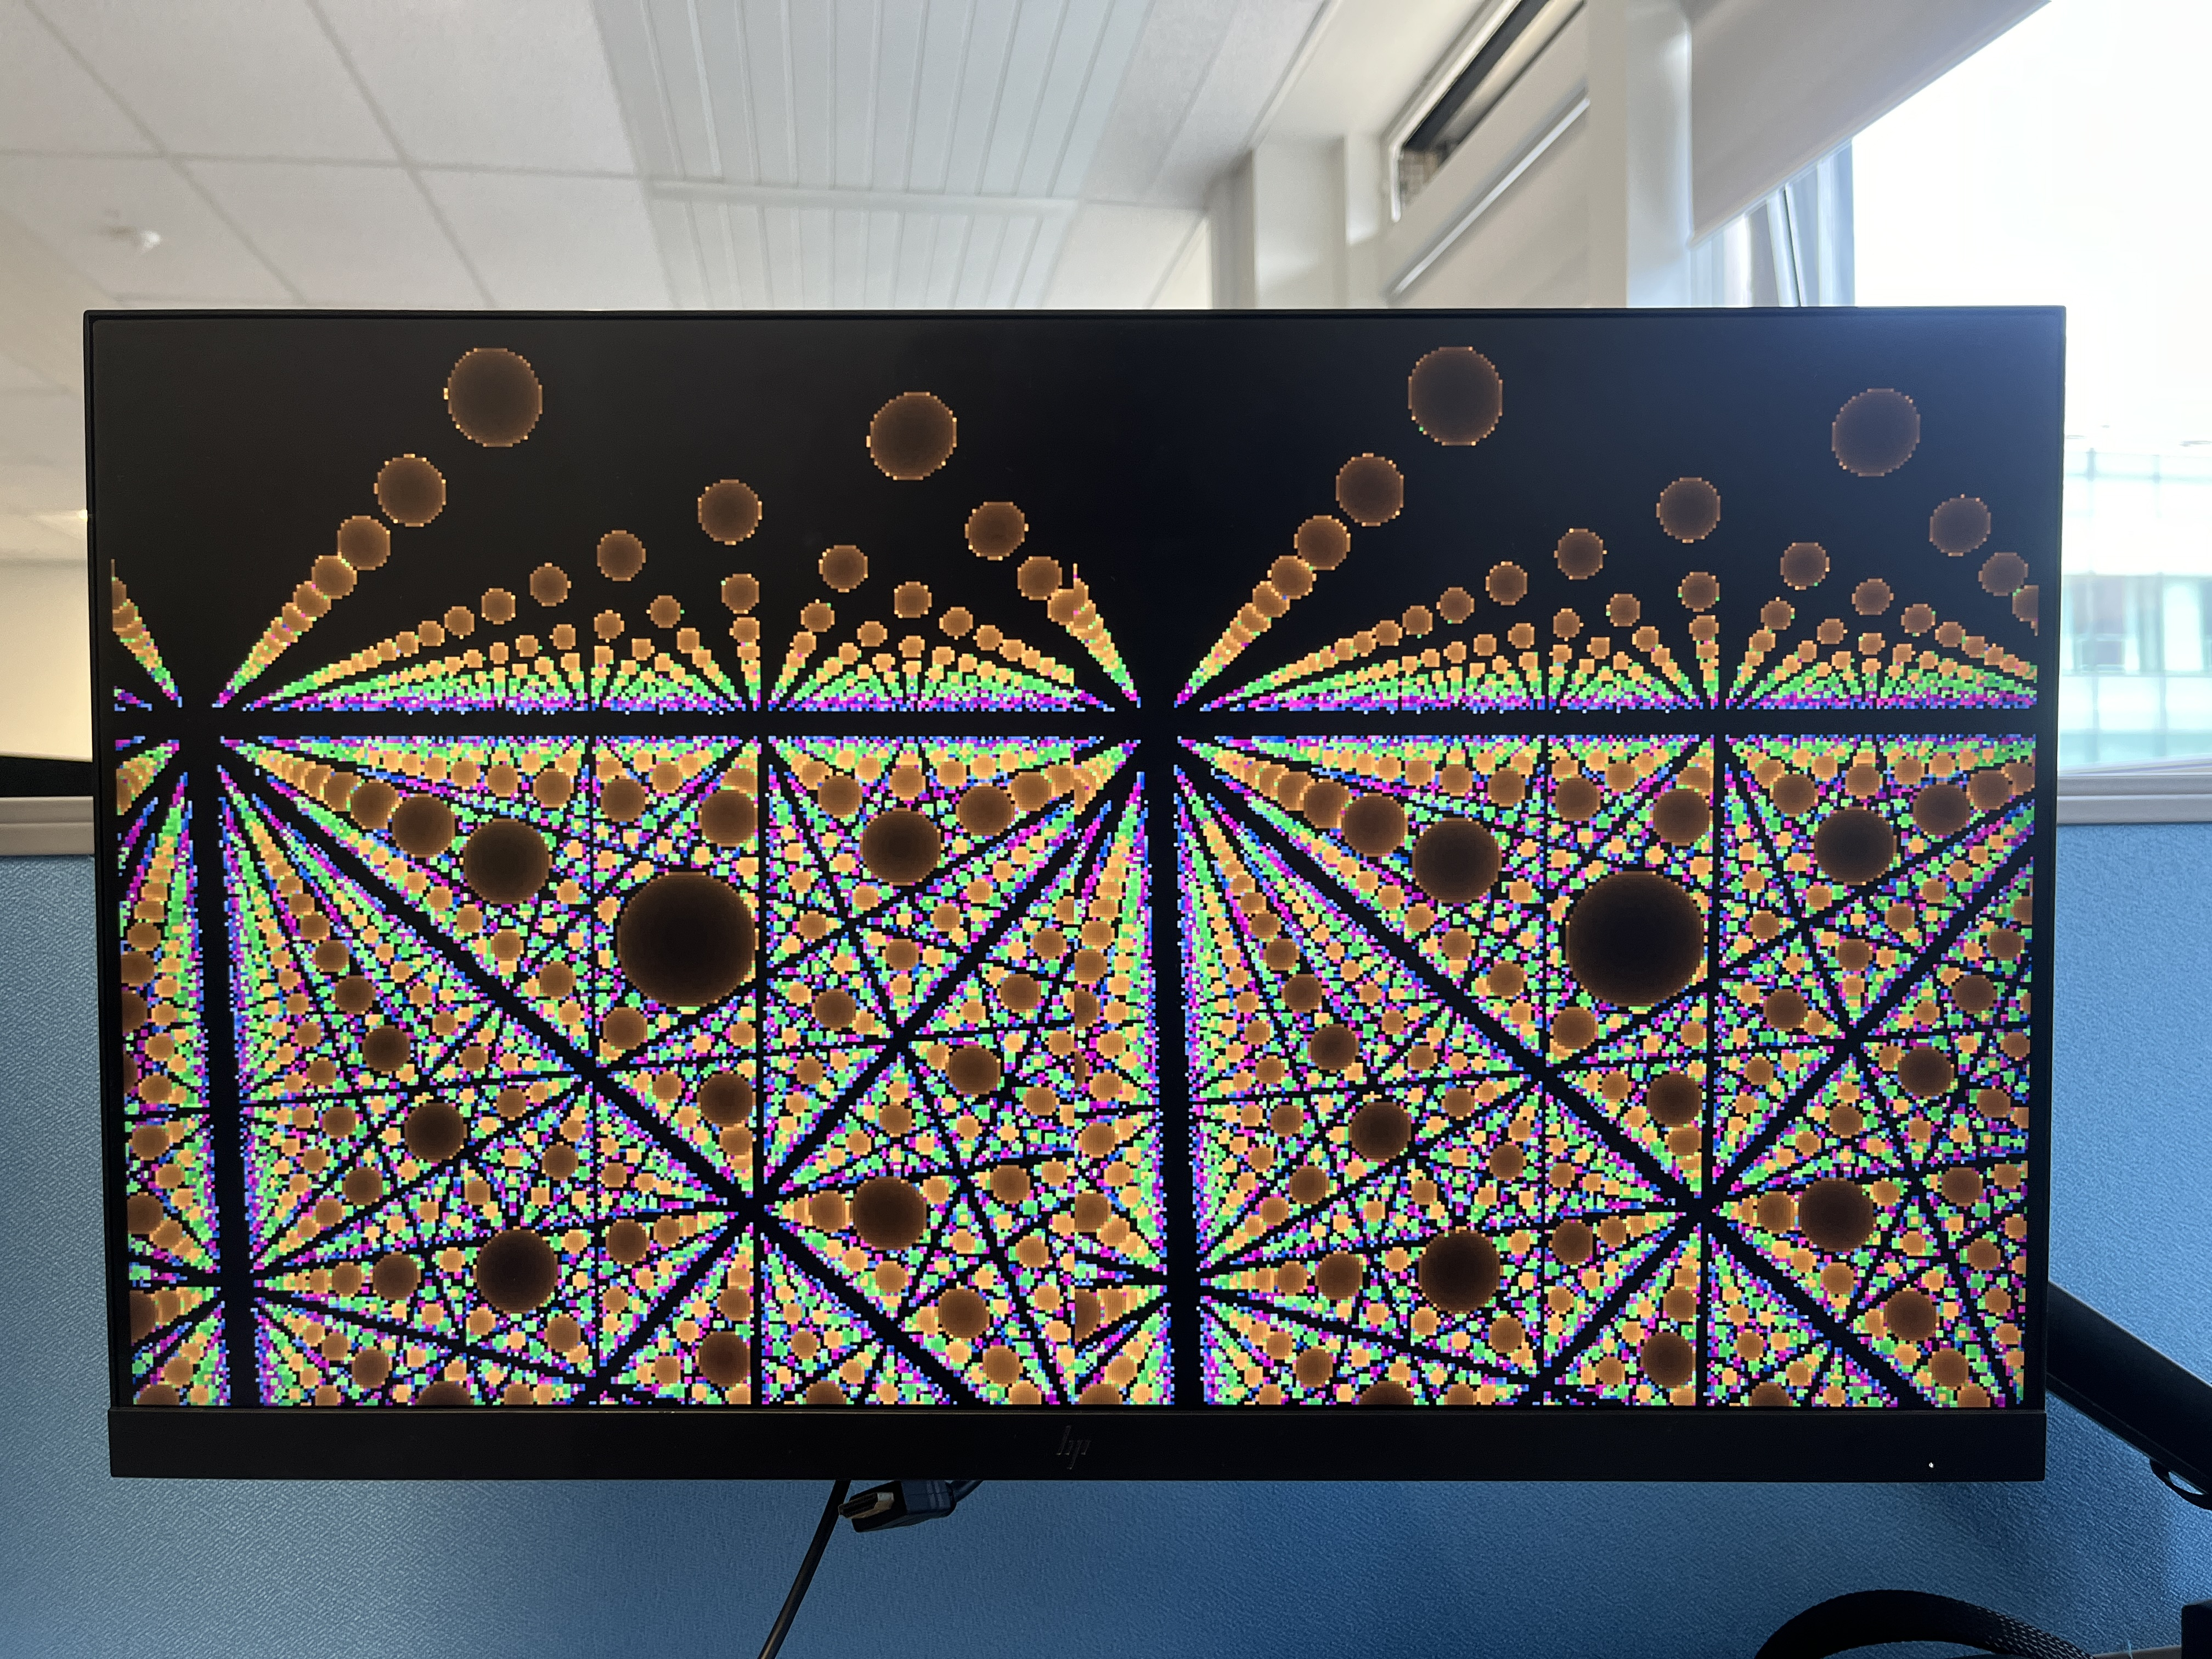
\includegraphics[width=\textwidth,height=0.28\textheight,keepaspectratio]{imgs/AppendixA/render_gyroid_spheres2_stereo.jpg}
    \caption{Infinite Spheres}
\end{subfigure}\hfill
\begin{subfigure}[b]{0.48\textwidth}
    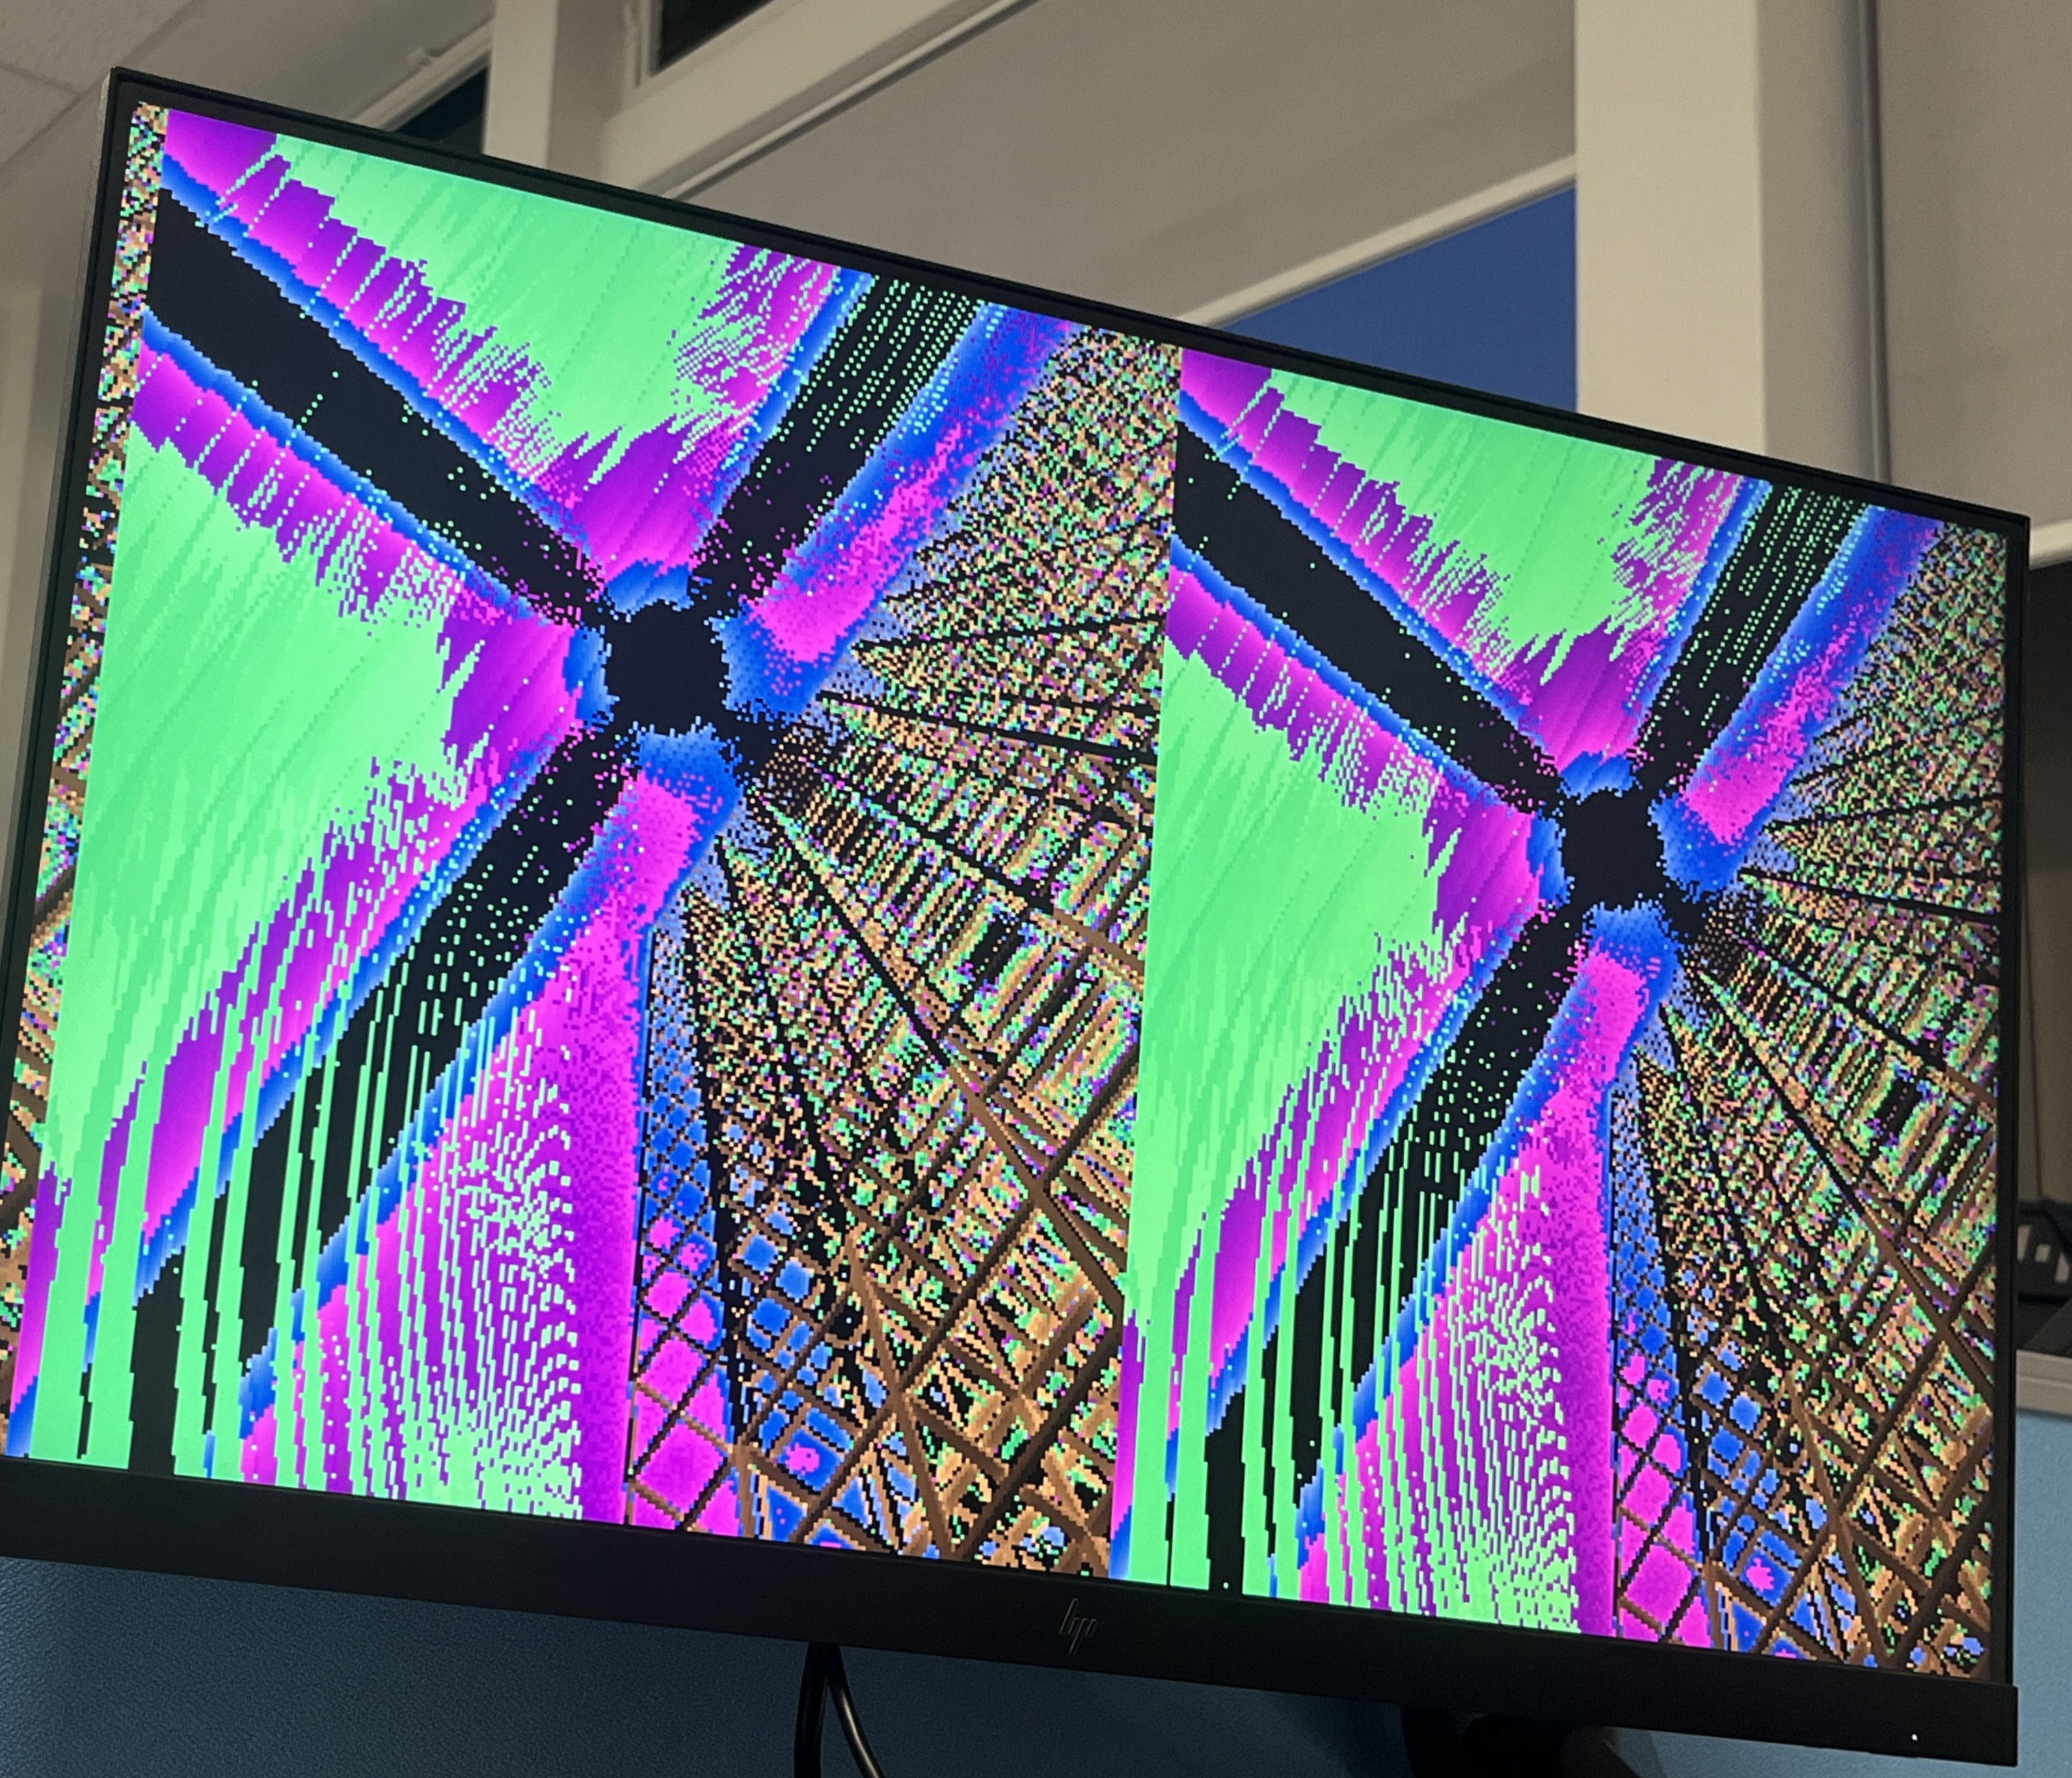
\includegraphics[width=\textwidth,height=0.28\textheight,keepaspectratio]{imgs/AppendixA/headset_photo_1.jpg}
    \caption{Assembled VR headset prototype, front view. FPGA friction-fitted into custom 3D-printed chassis.}
\end{subfigure}
\caption{Stereoscopic render gallery II: Mandelbox variants and assembled headset.}
\end{figure}

\clearpage

% ----------------------------------------------------------------
%  Page 3 — New scaffold stereo board photos (5) + headset photo 2
% ----------------------------------------------------------------
\begin{figure}[H]
\vspace*{-0.5cm}
\centering
\begin{subfigure}[b]{0.48\textwidth}
    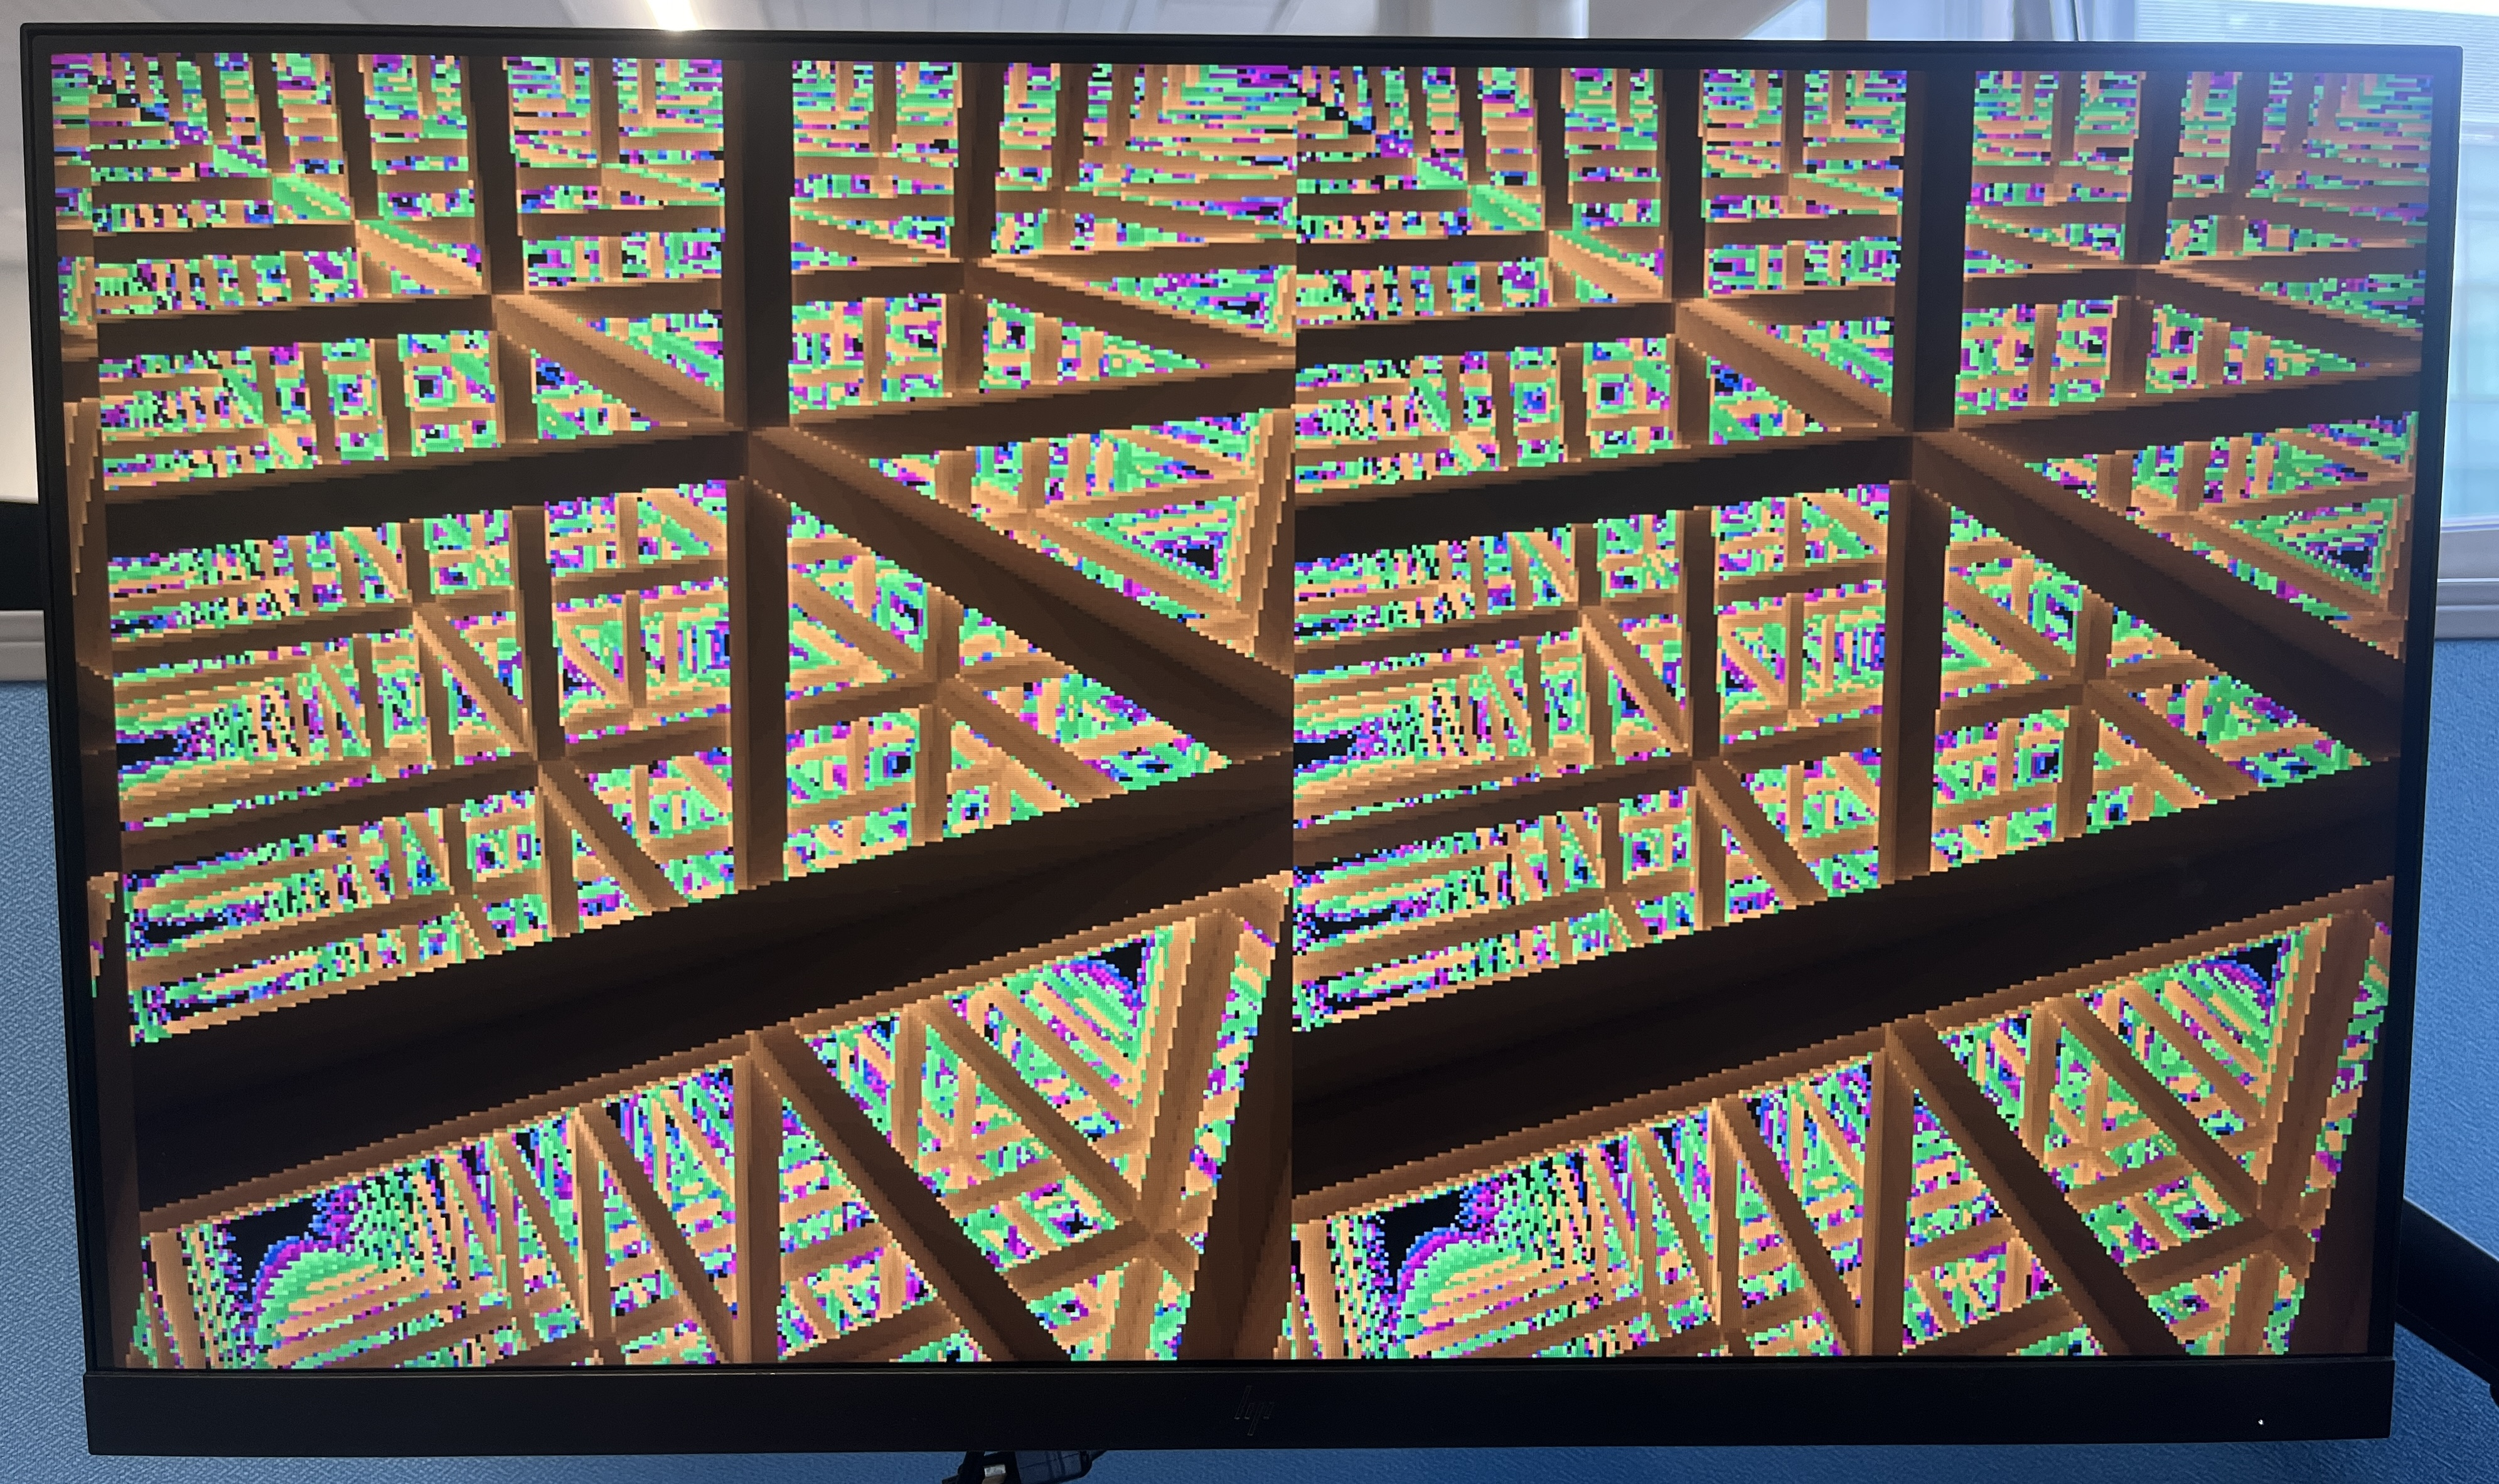
\includegraphics[width=\textwidth,height=0.28\textheight,keepaspectratio]{imgs/AppendixA/render_scaffold_overhead_stereo.jpg}
    \caption{Scaffold box-frame from an oblique overhead angle. Infinite lattice depth visible across the stereo pair.}
\end{subfigure}\hfill
\begin{subfigure}[b]{0.48\textwidth}
    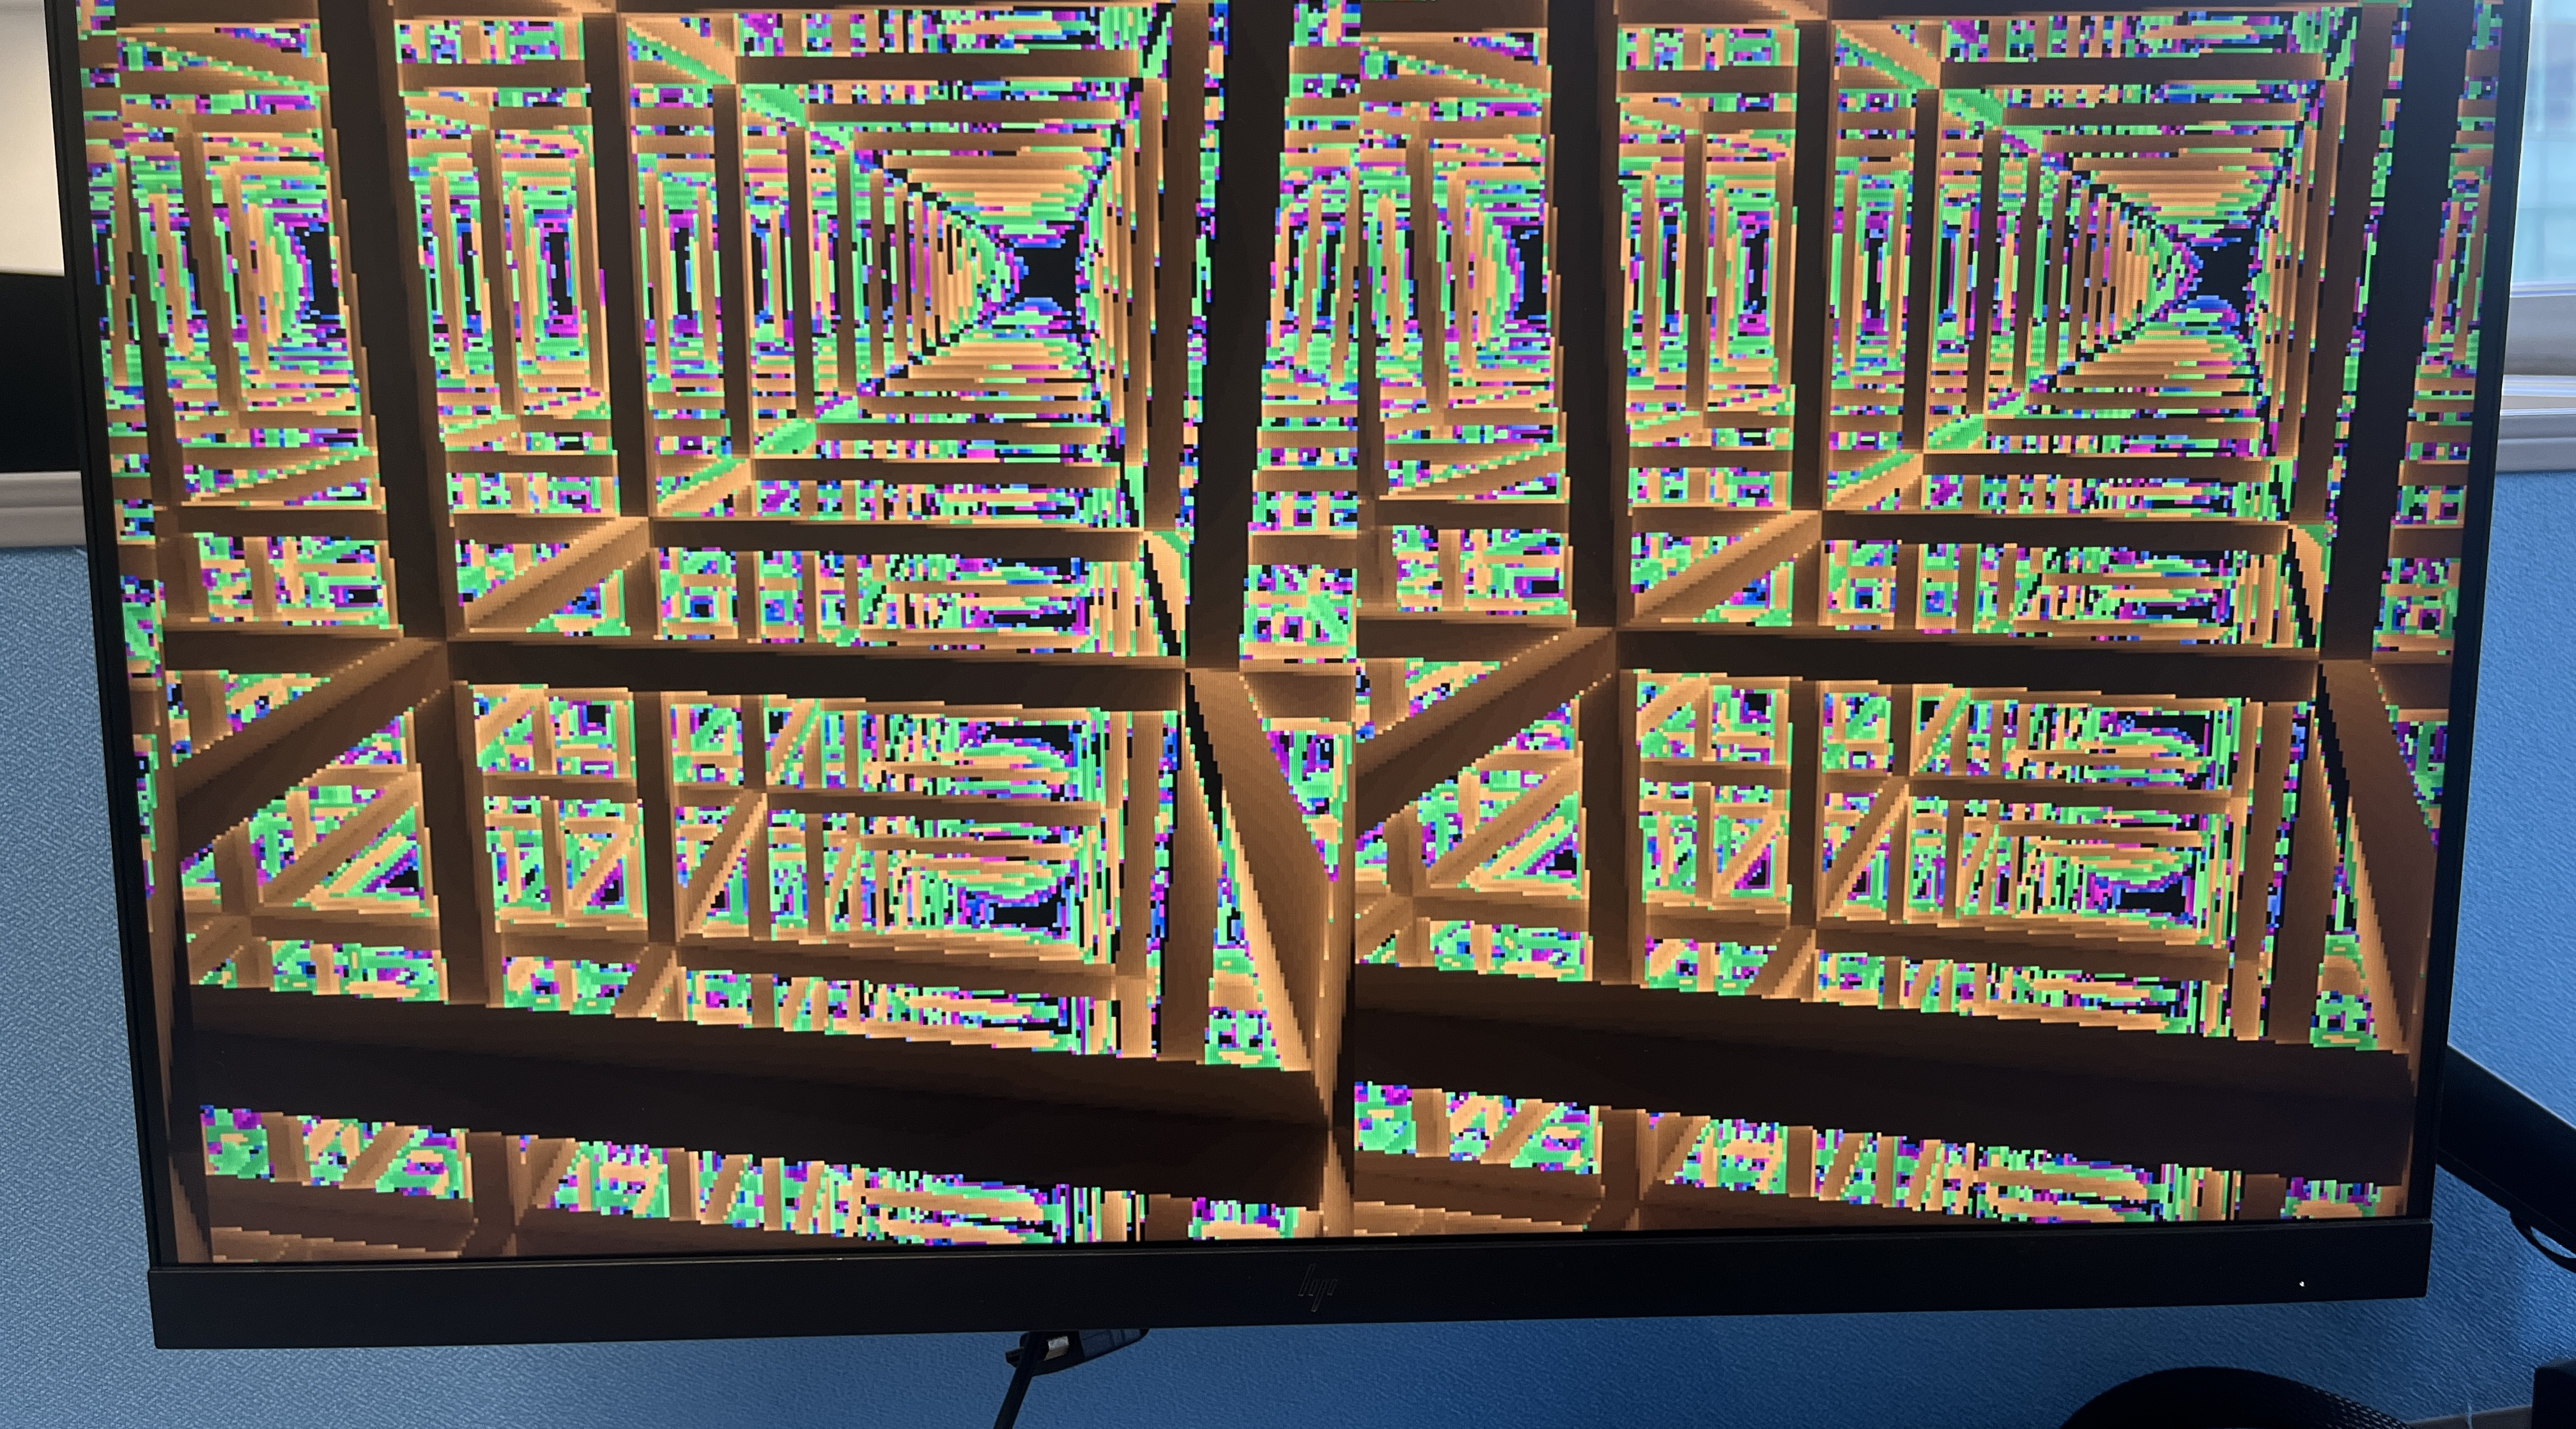
\includegraphics[width=\textwidth,height=0.28\textheight,keepaspectratio]{imgs/AppendixA/render_scaffold_tunnel_stereo.jpg}
    \caption{Scaffold tunnel, looking straight down a corridor. Iteration colourmap highlights infinite recession.}
\end{subfigure}

\vfill

\begin{subfigure}[b]{0.48\textwidth}
    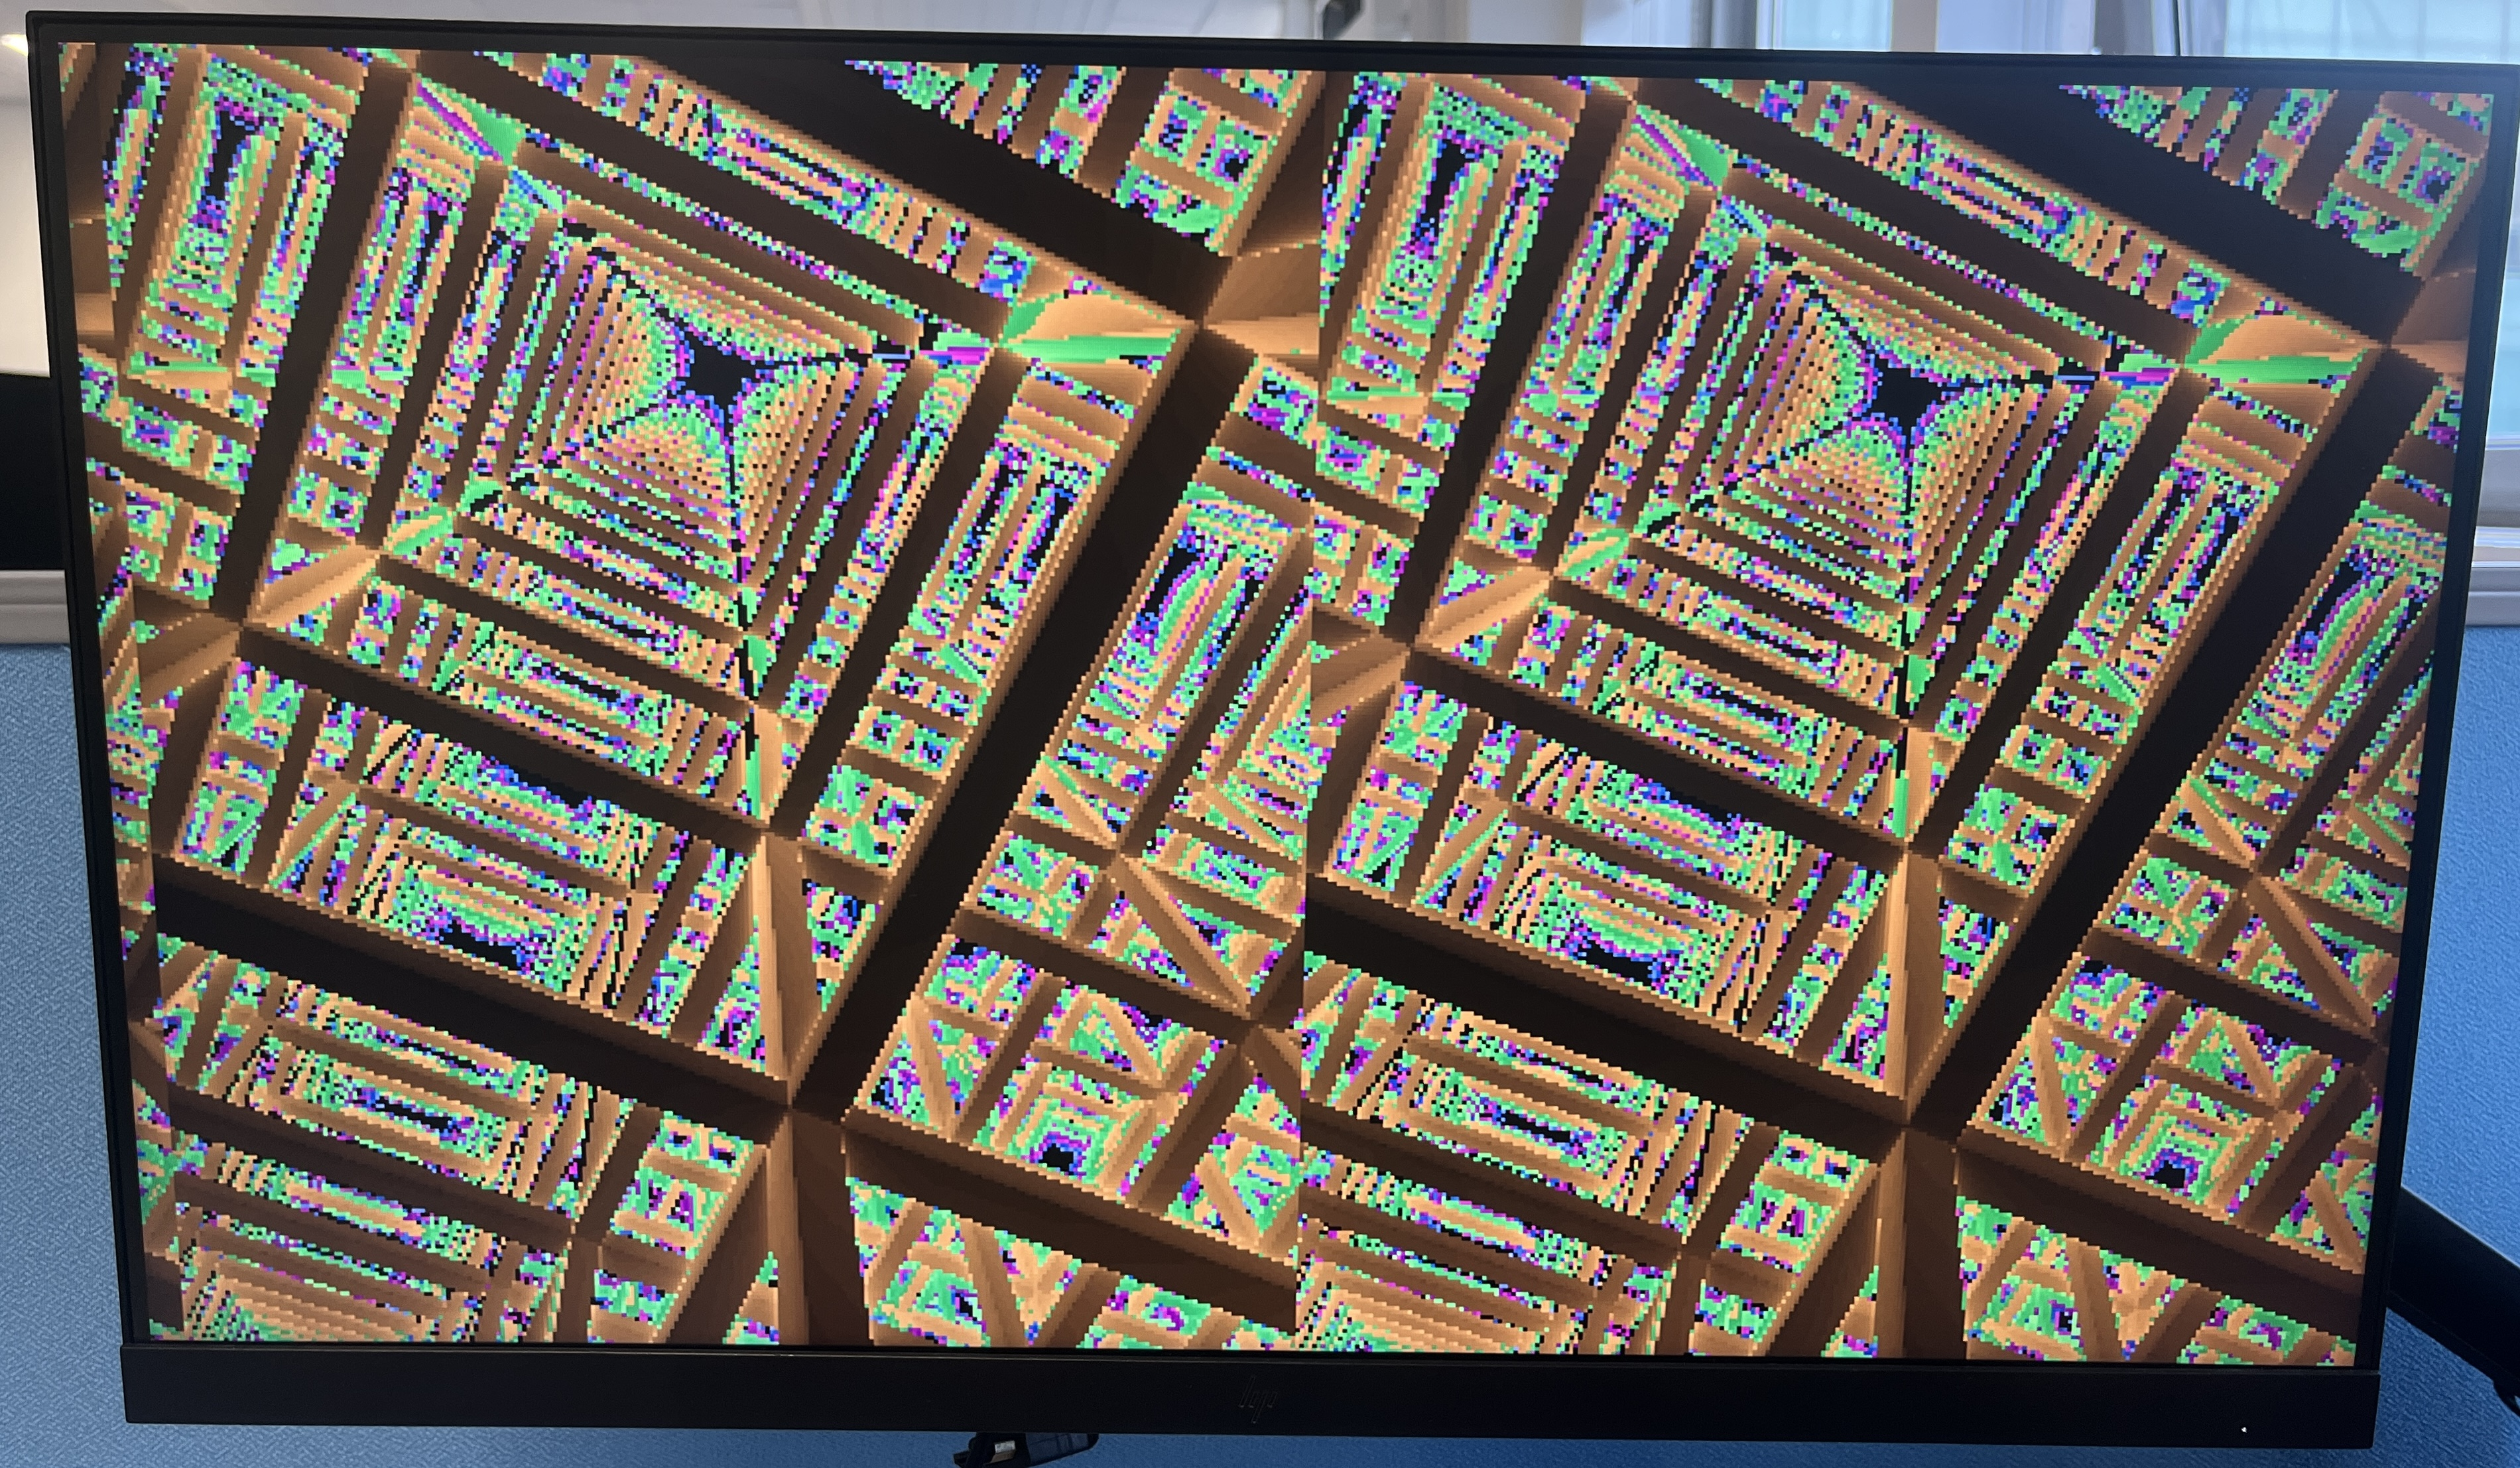
\includegraphics[width=\textwidth,height=0.28\textheight,keepaspectratio]{imgs/AppendixA/render_scaffold_zenith_stereo.jpg}
    \caption{Scaffold zenith view: camera looking straight up through nested box frames into infinite depth.}
\end{subfigure}\hfill
\begin{subfigure}[b]{0.48\textwidth}
    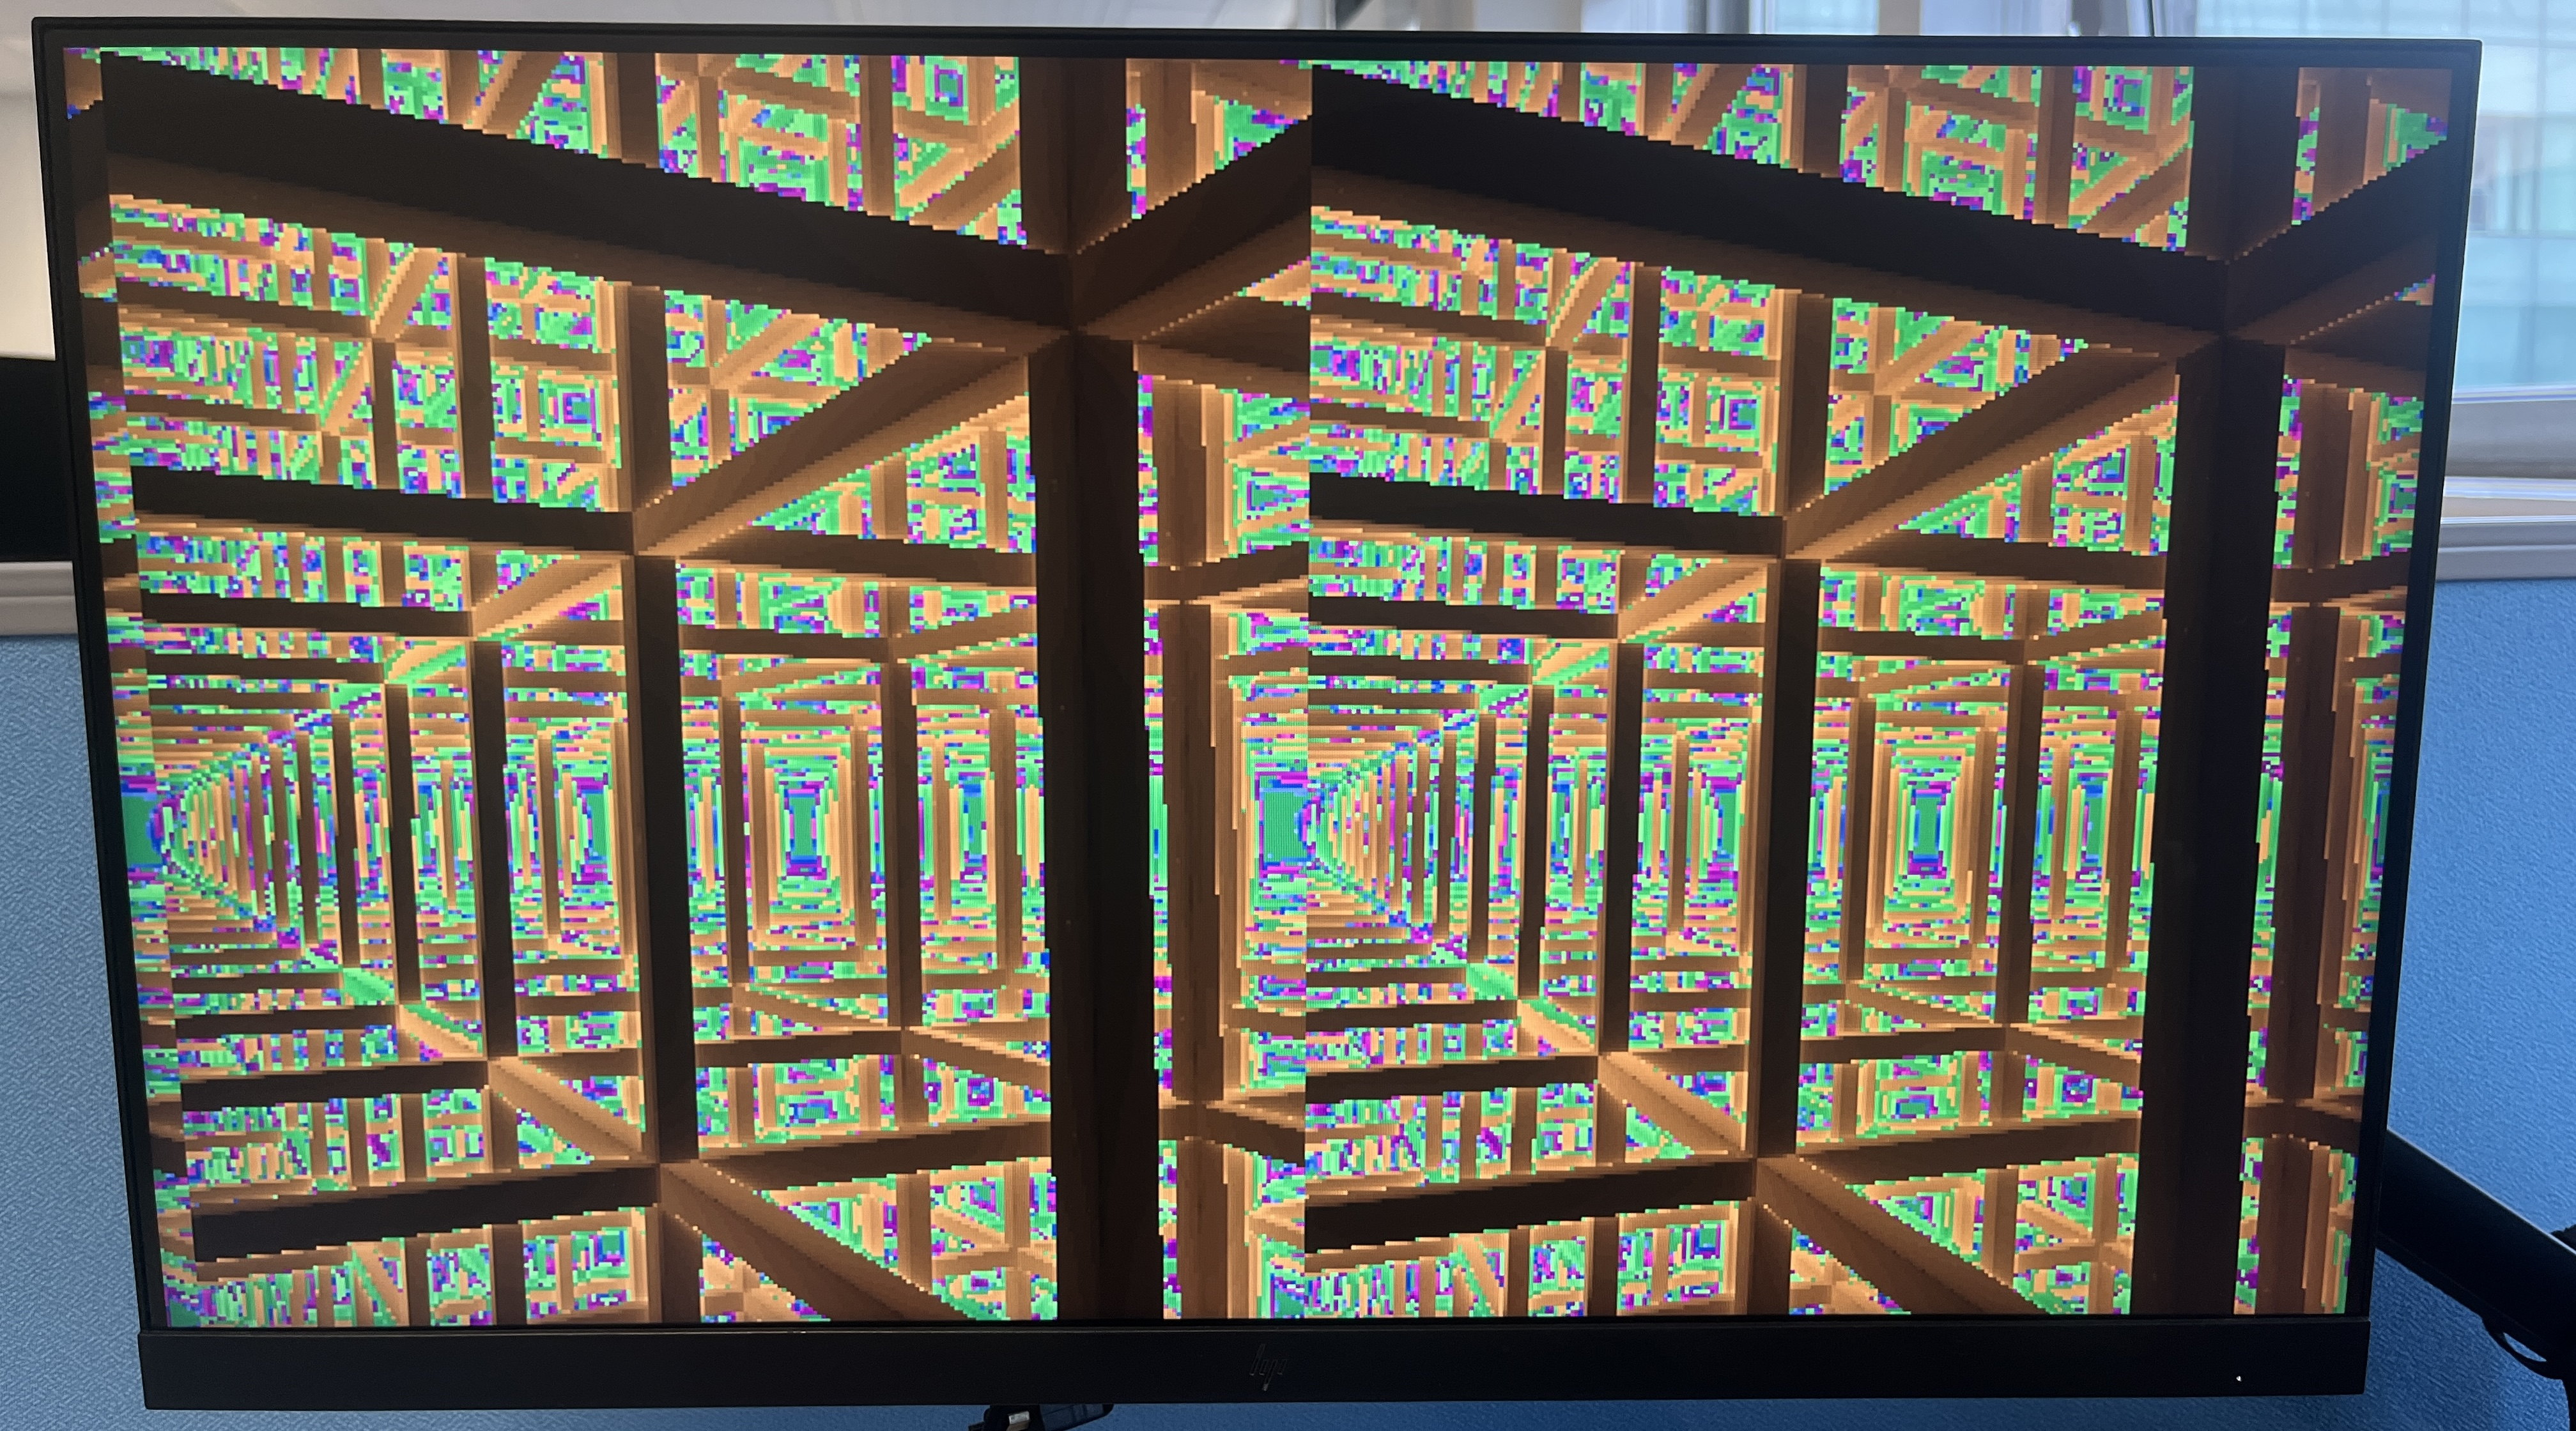
\includegraphics[width=\textwidth,height=0.28\textheight,keepaspectratio]{imgs/AppendixA/render_scaffold_corridor_stereo.jpg}
    \caption{Scaffold corridor, angled stereo shot. Space repetition cell boundaries clearly delineated.}
\end{subfigure}

\vfill

\begin{subfigure}[b]{0.48\textwidth}
    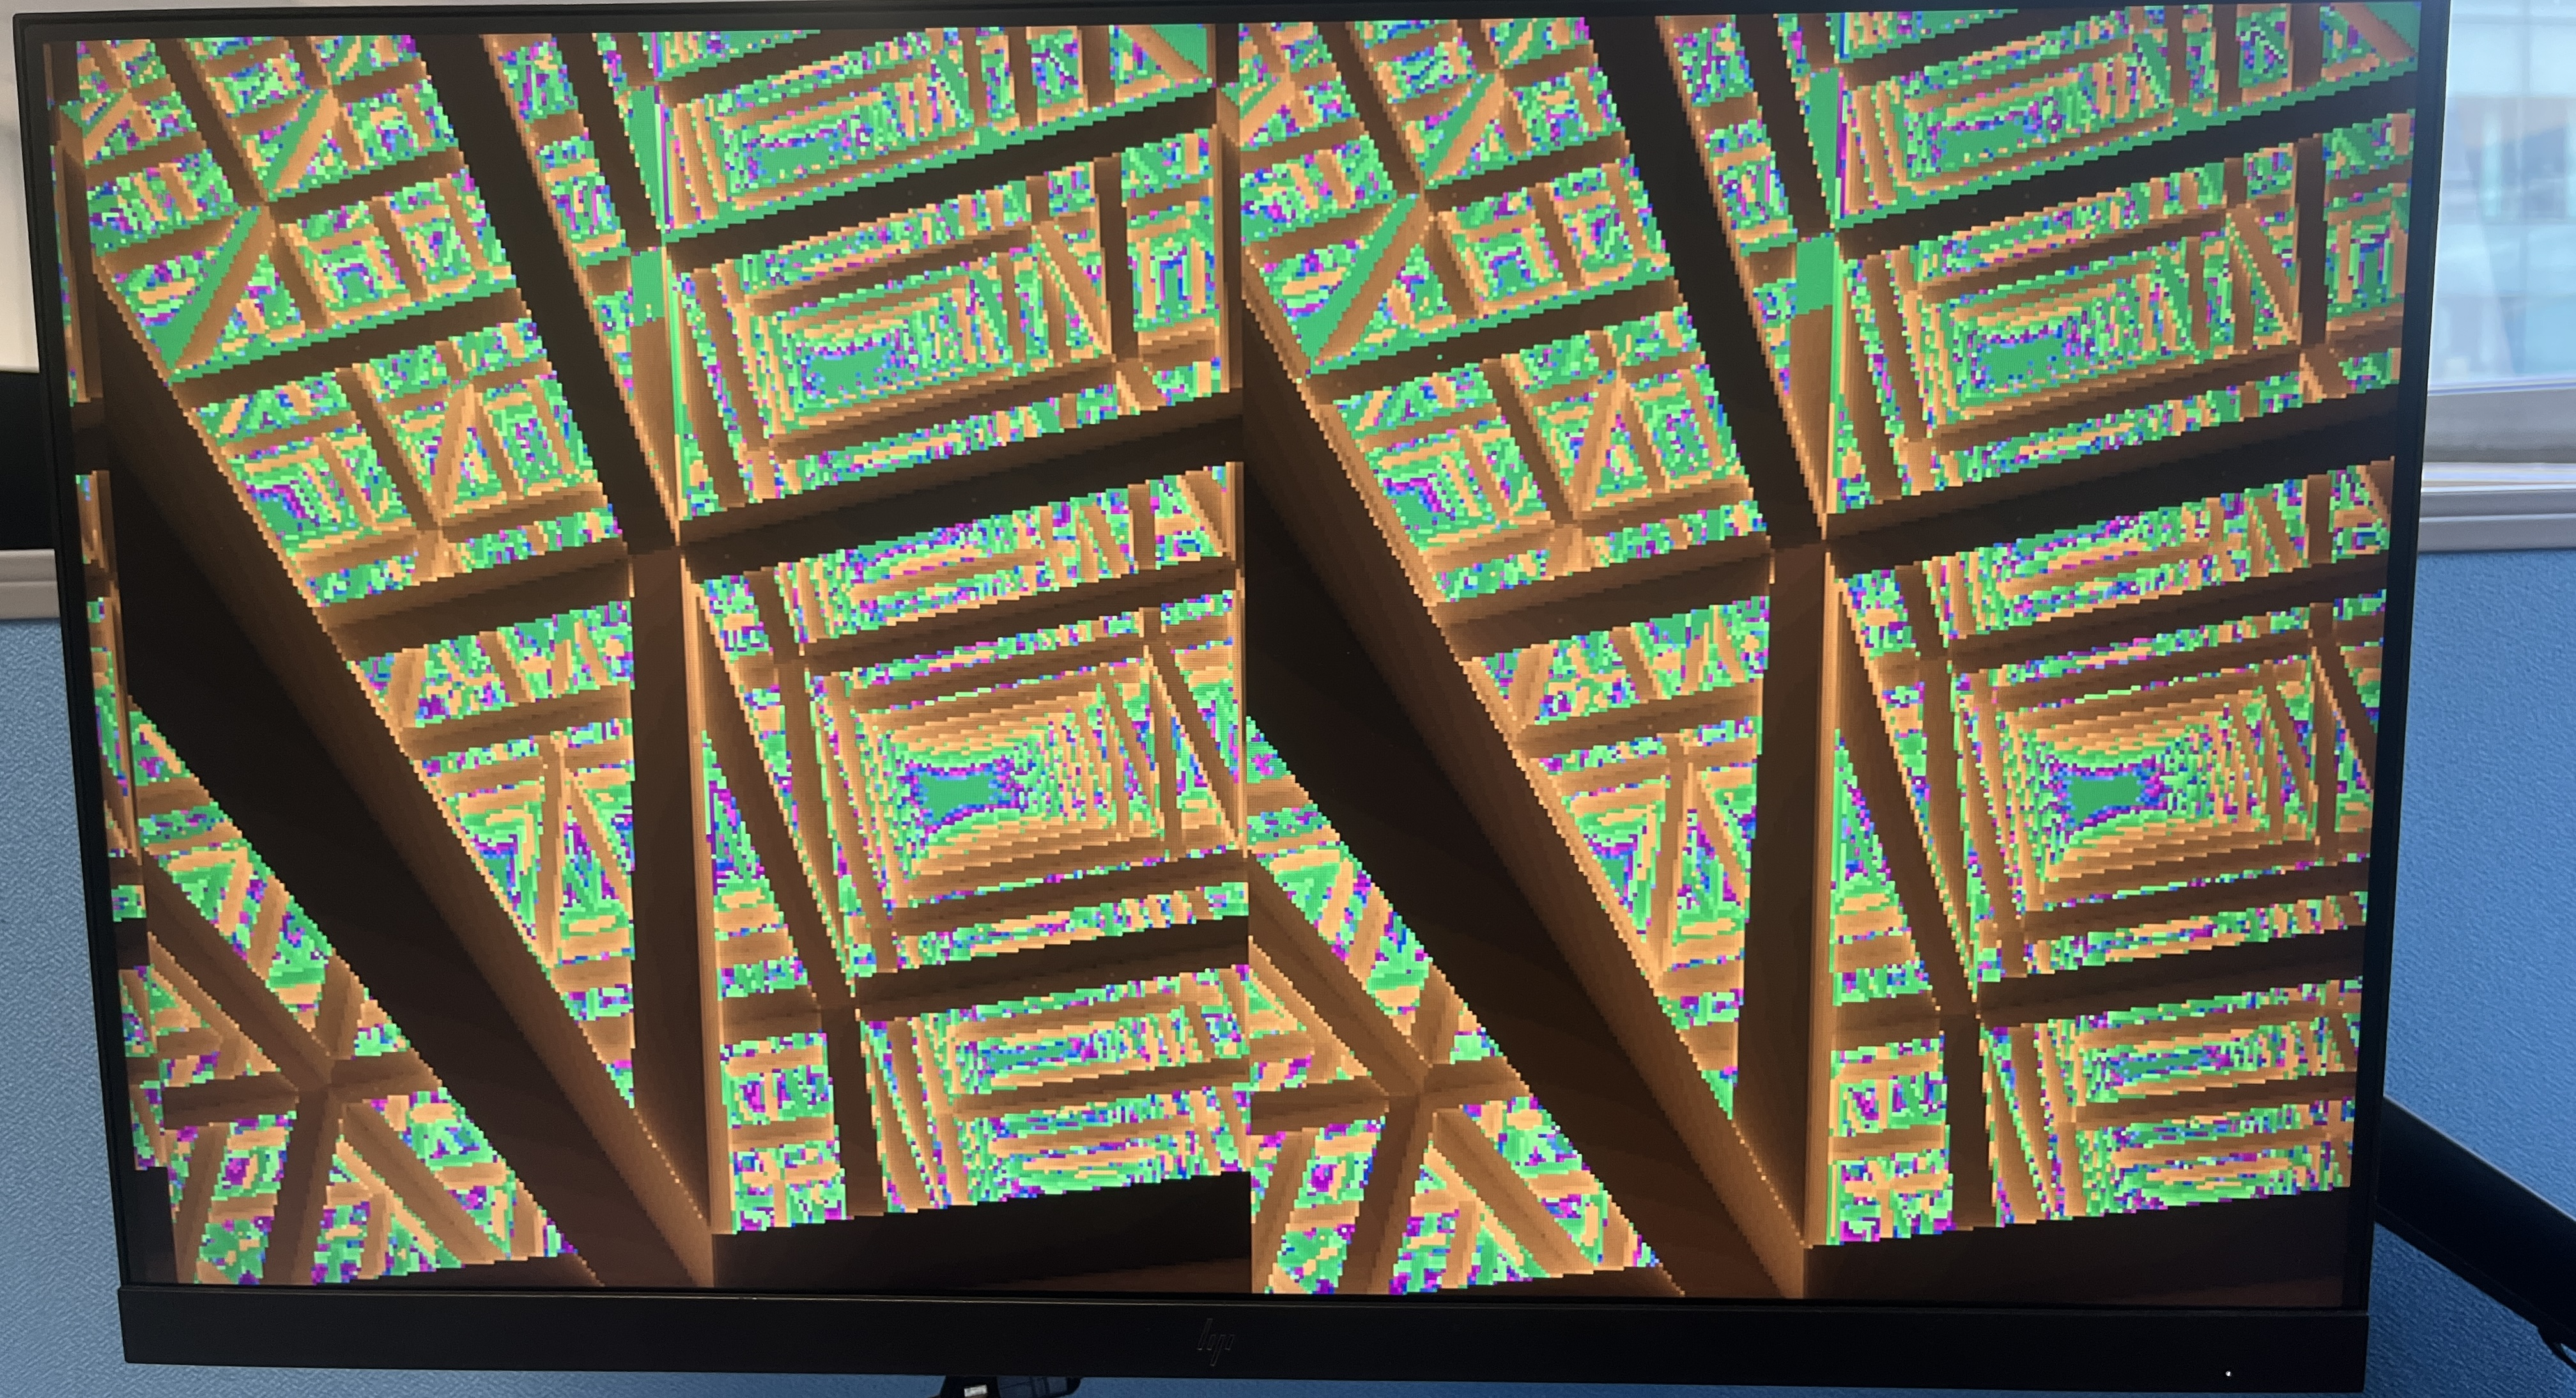
\includegraphics[width=\textwidth,height=0.28\textheight,keepaspectratio]{imgs/AppendixA/render_scaffold_diagonal_stereo.jpg}
    \caption{Scaffold diagonal view, close to the frame geometry. FP27 precision resolves fine strut edges without aliasing.}
\end{subfigure}\hfill
\begin{subfigure}[b]{0.48\textwidth}
    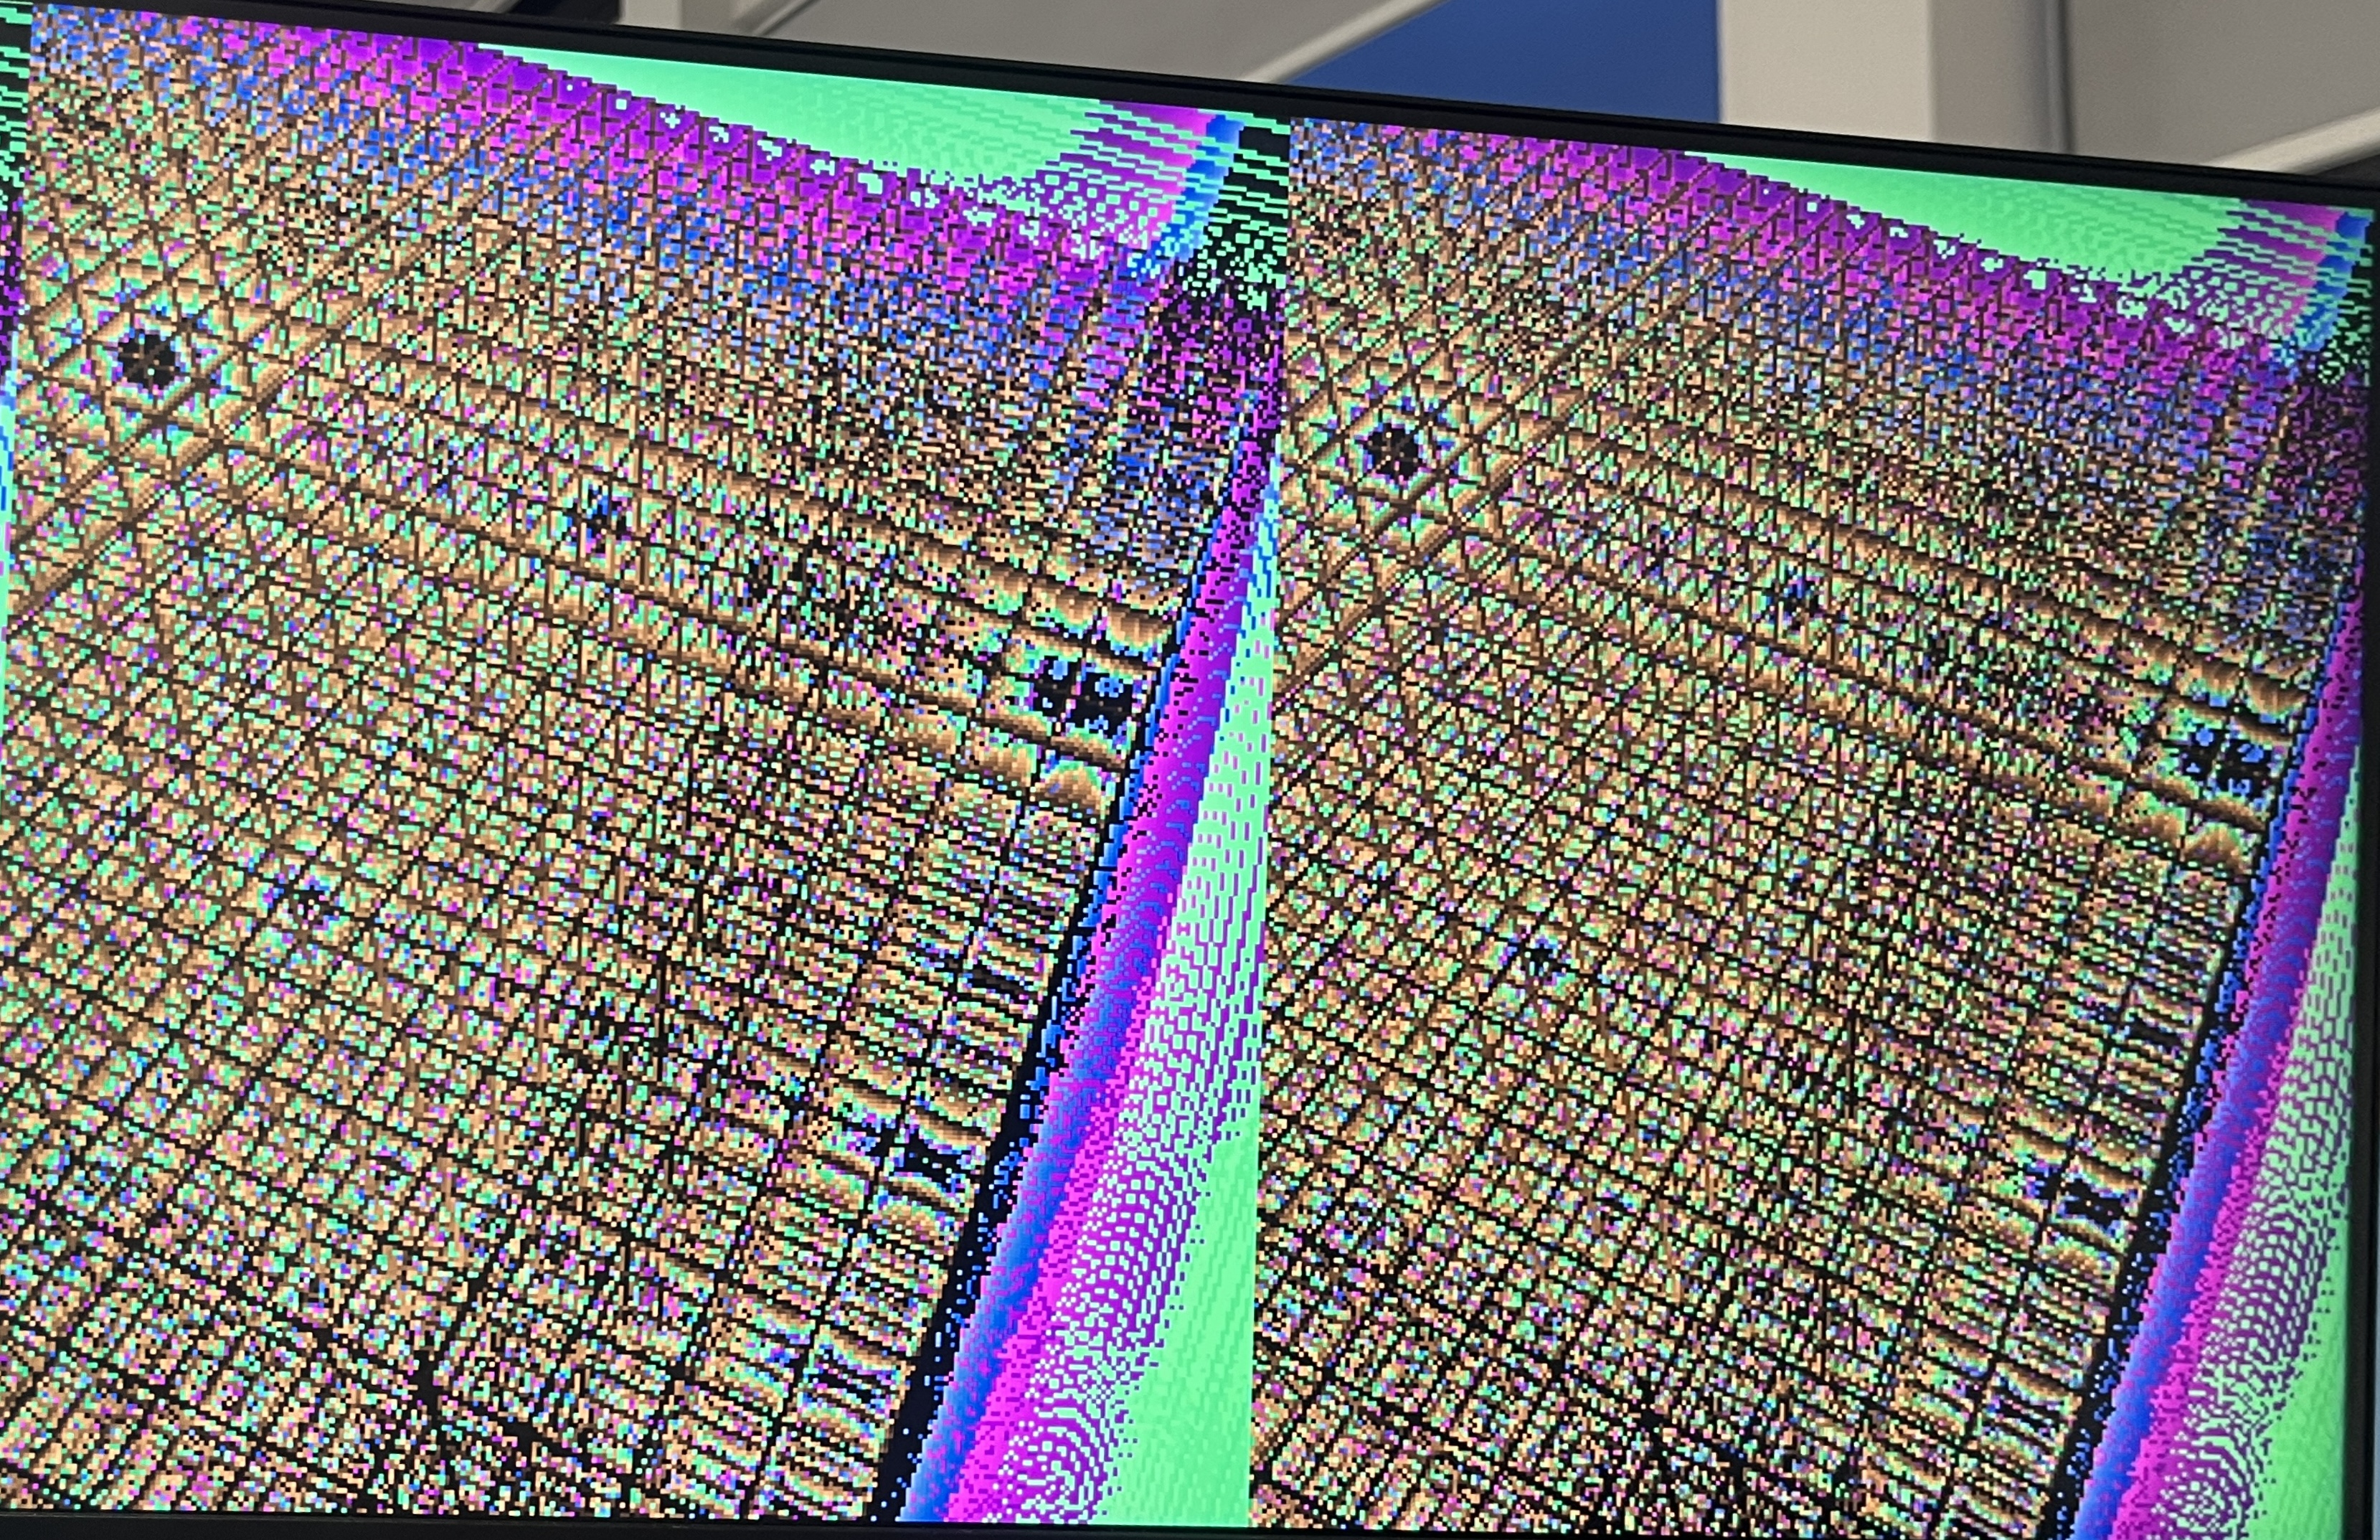
\includegraphics[width=\textwidth,height=0.28\textheight,keepaspectratio]{imgs/AppendixA/headset_photo_2.jpg}
    \caption{Assembled VR headset, side profile. Quest~2 headstrap adapter and 90-degree HDMI cable routing visible.}
\end{subfigure}
\caption{Stereoscopic render gallery III, scaffold scene perspectives on physical board.}
\end{figure}

\clearpage

% ----------------------------------------------------------------
%  Page 4 — GLSL software reference renders: scaffold interior views
% ----------------------------------------------------------------
\begin{figure}[H]
\vspace*{-0.5cm}
\centering
\begin{subfigure}[b]{0.48\textwidth}
    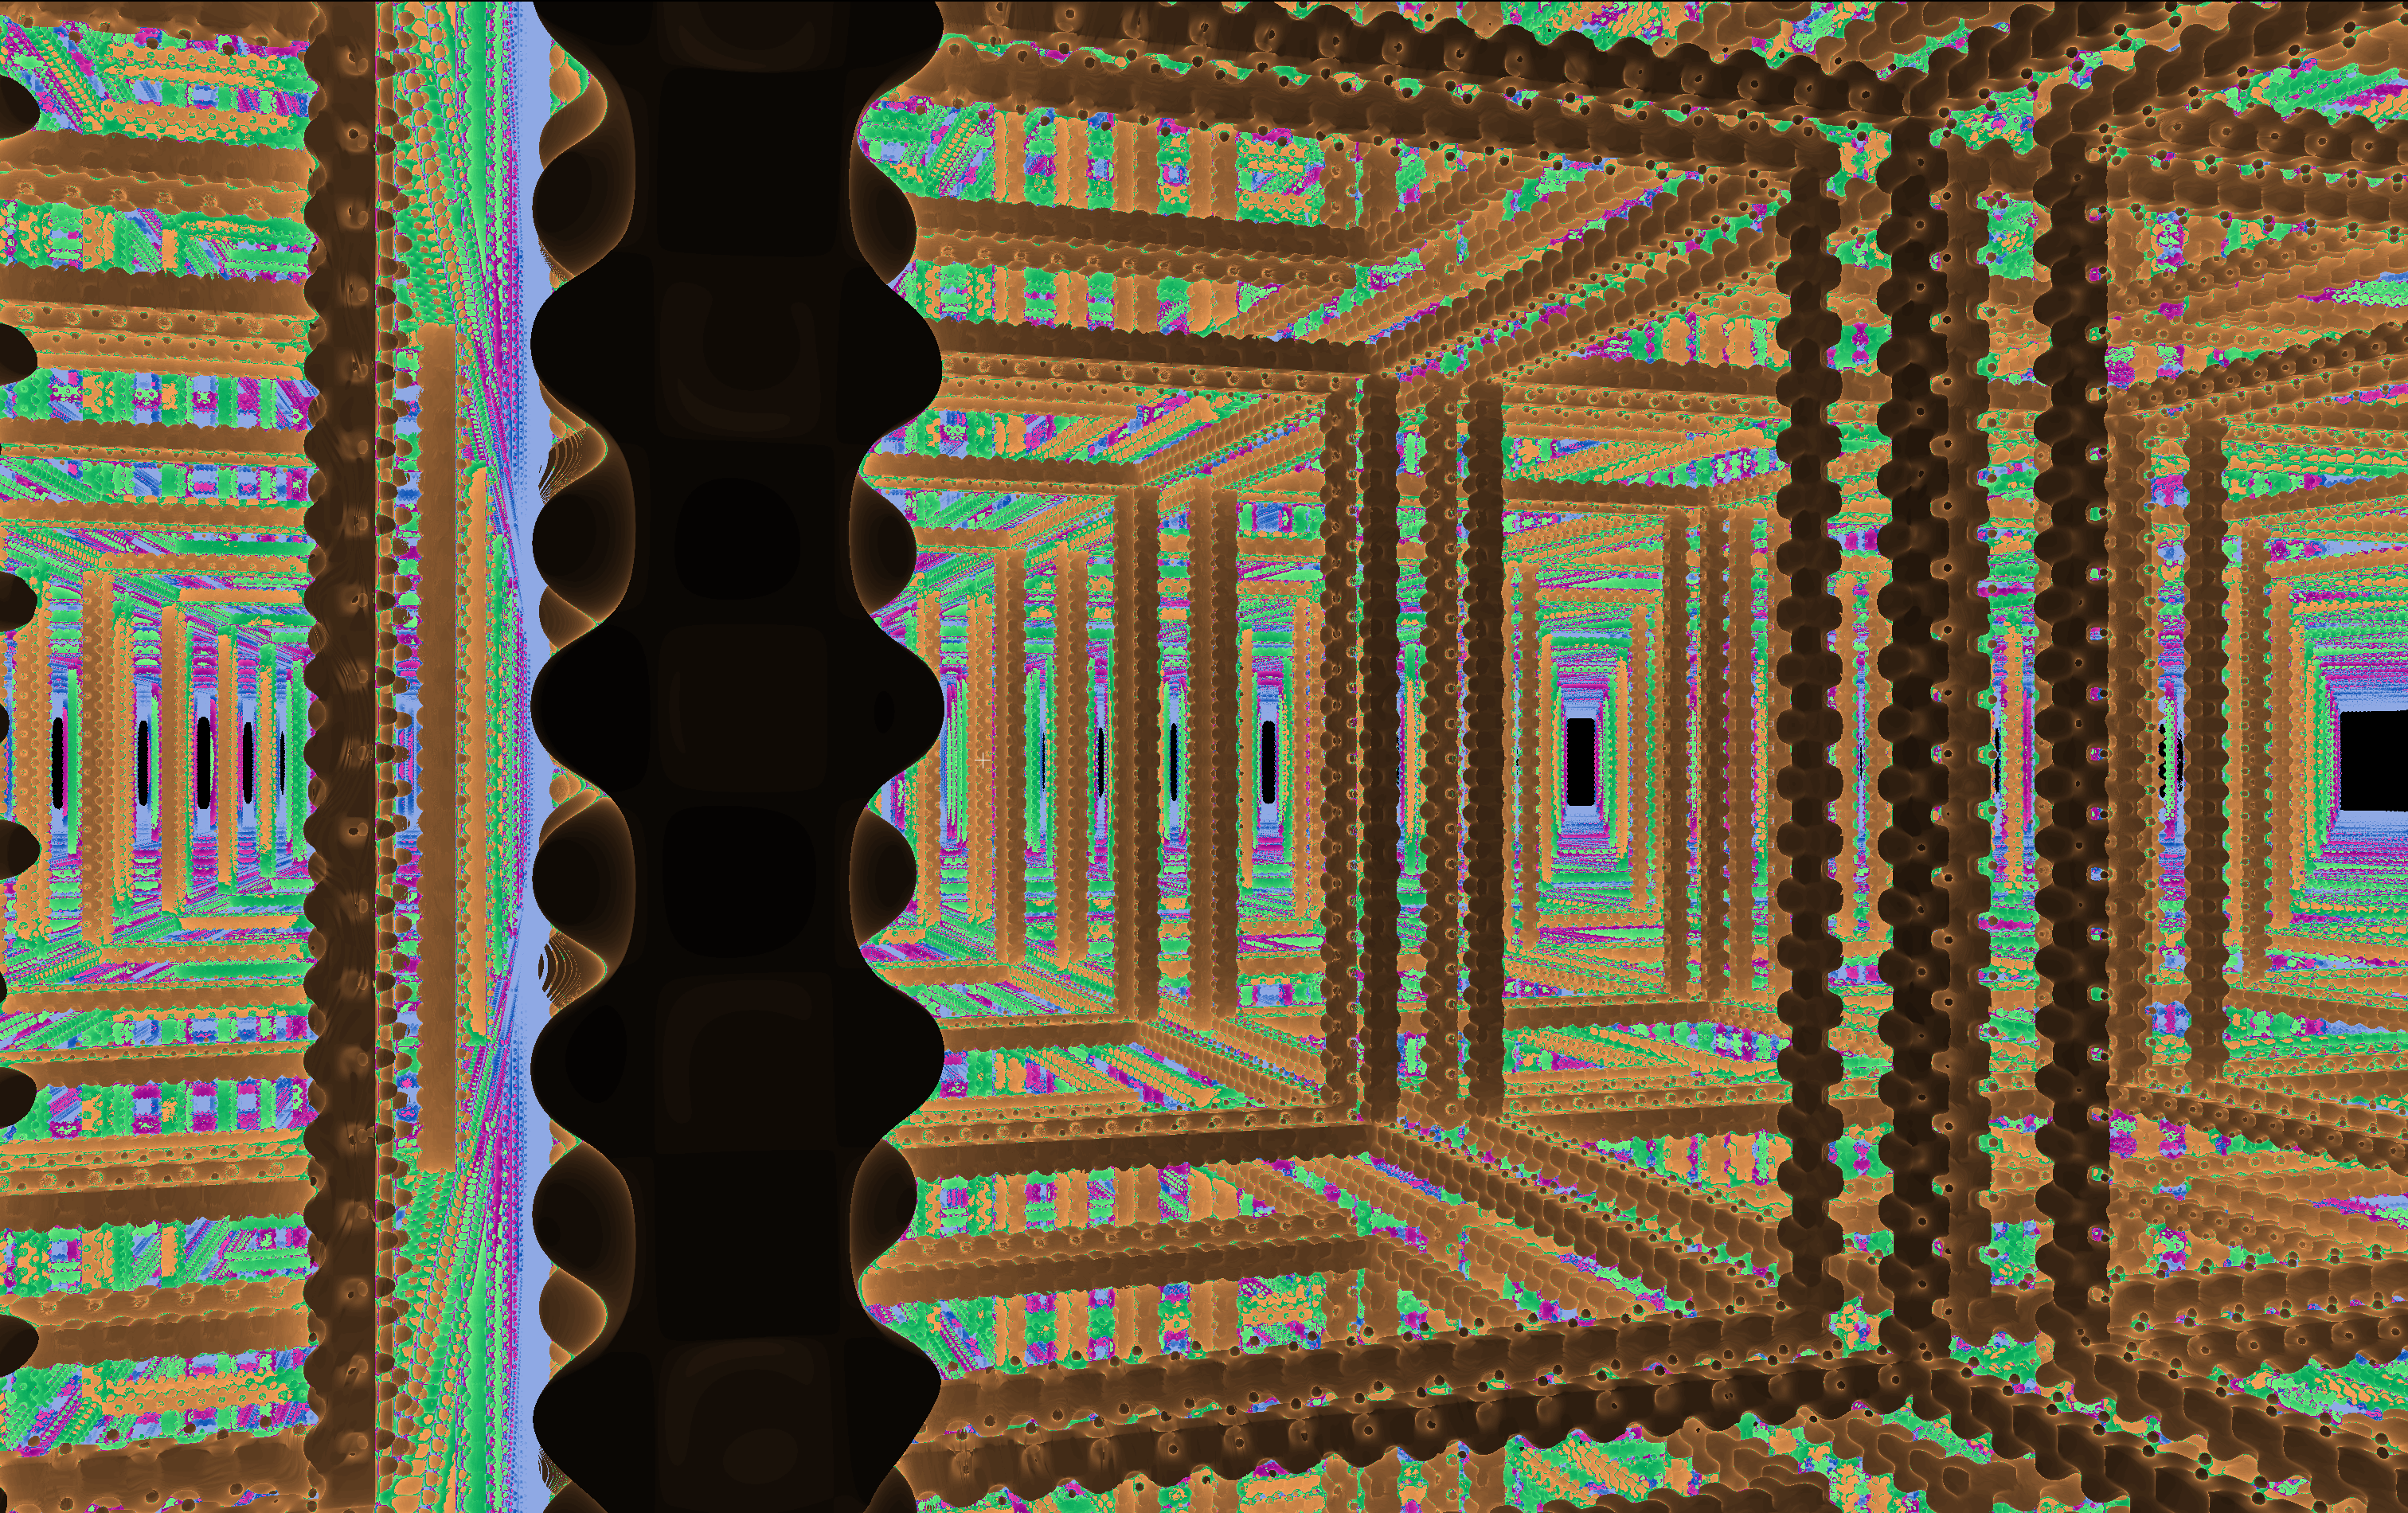
\includegraphics[width=\textwidth,height=0.28\textheight,keepaspectratio]{imgs/AppendixA/render_scaffold_glsl_pillar.png}
    \caption{GLSL reference renderer, scaffold interior with twisted strut column in foreground, infinite depth field.}
\end{subfigure}\hfill
\begin{subfigure}[b]{0.48\textwidth}
    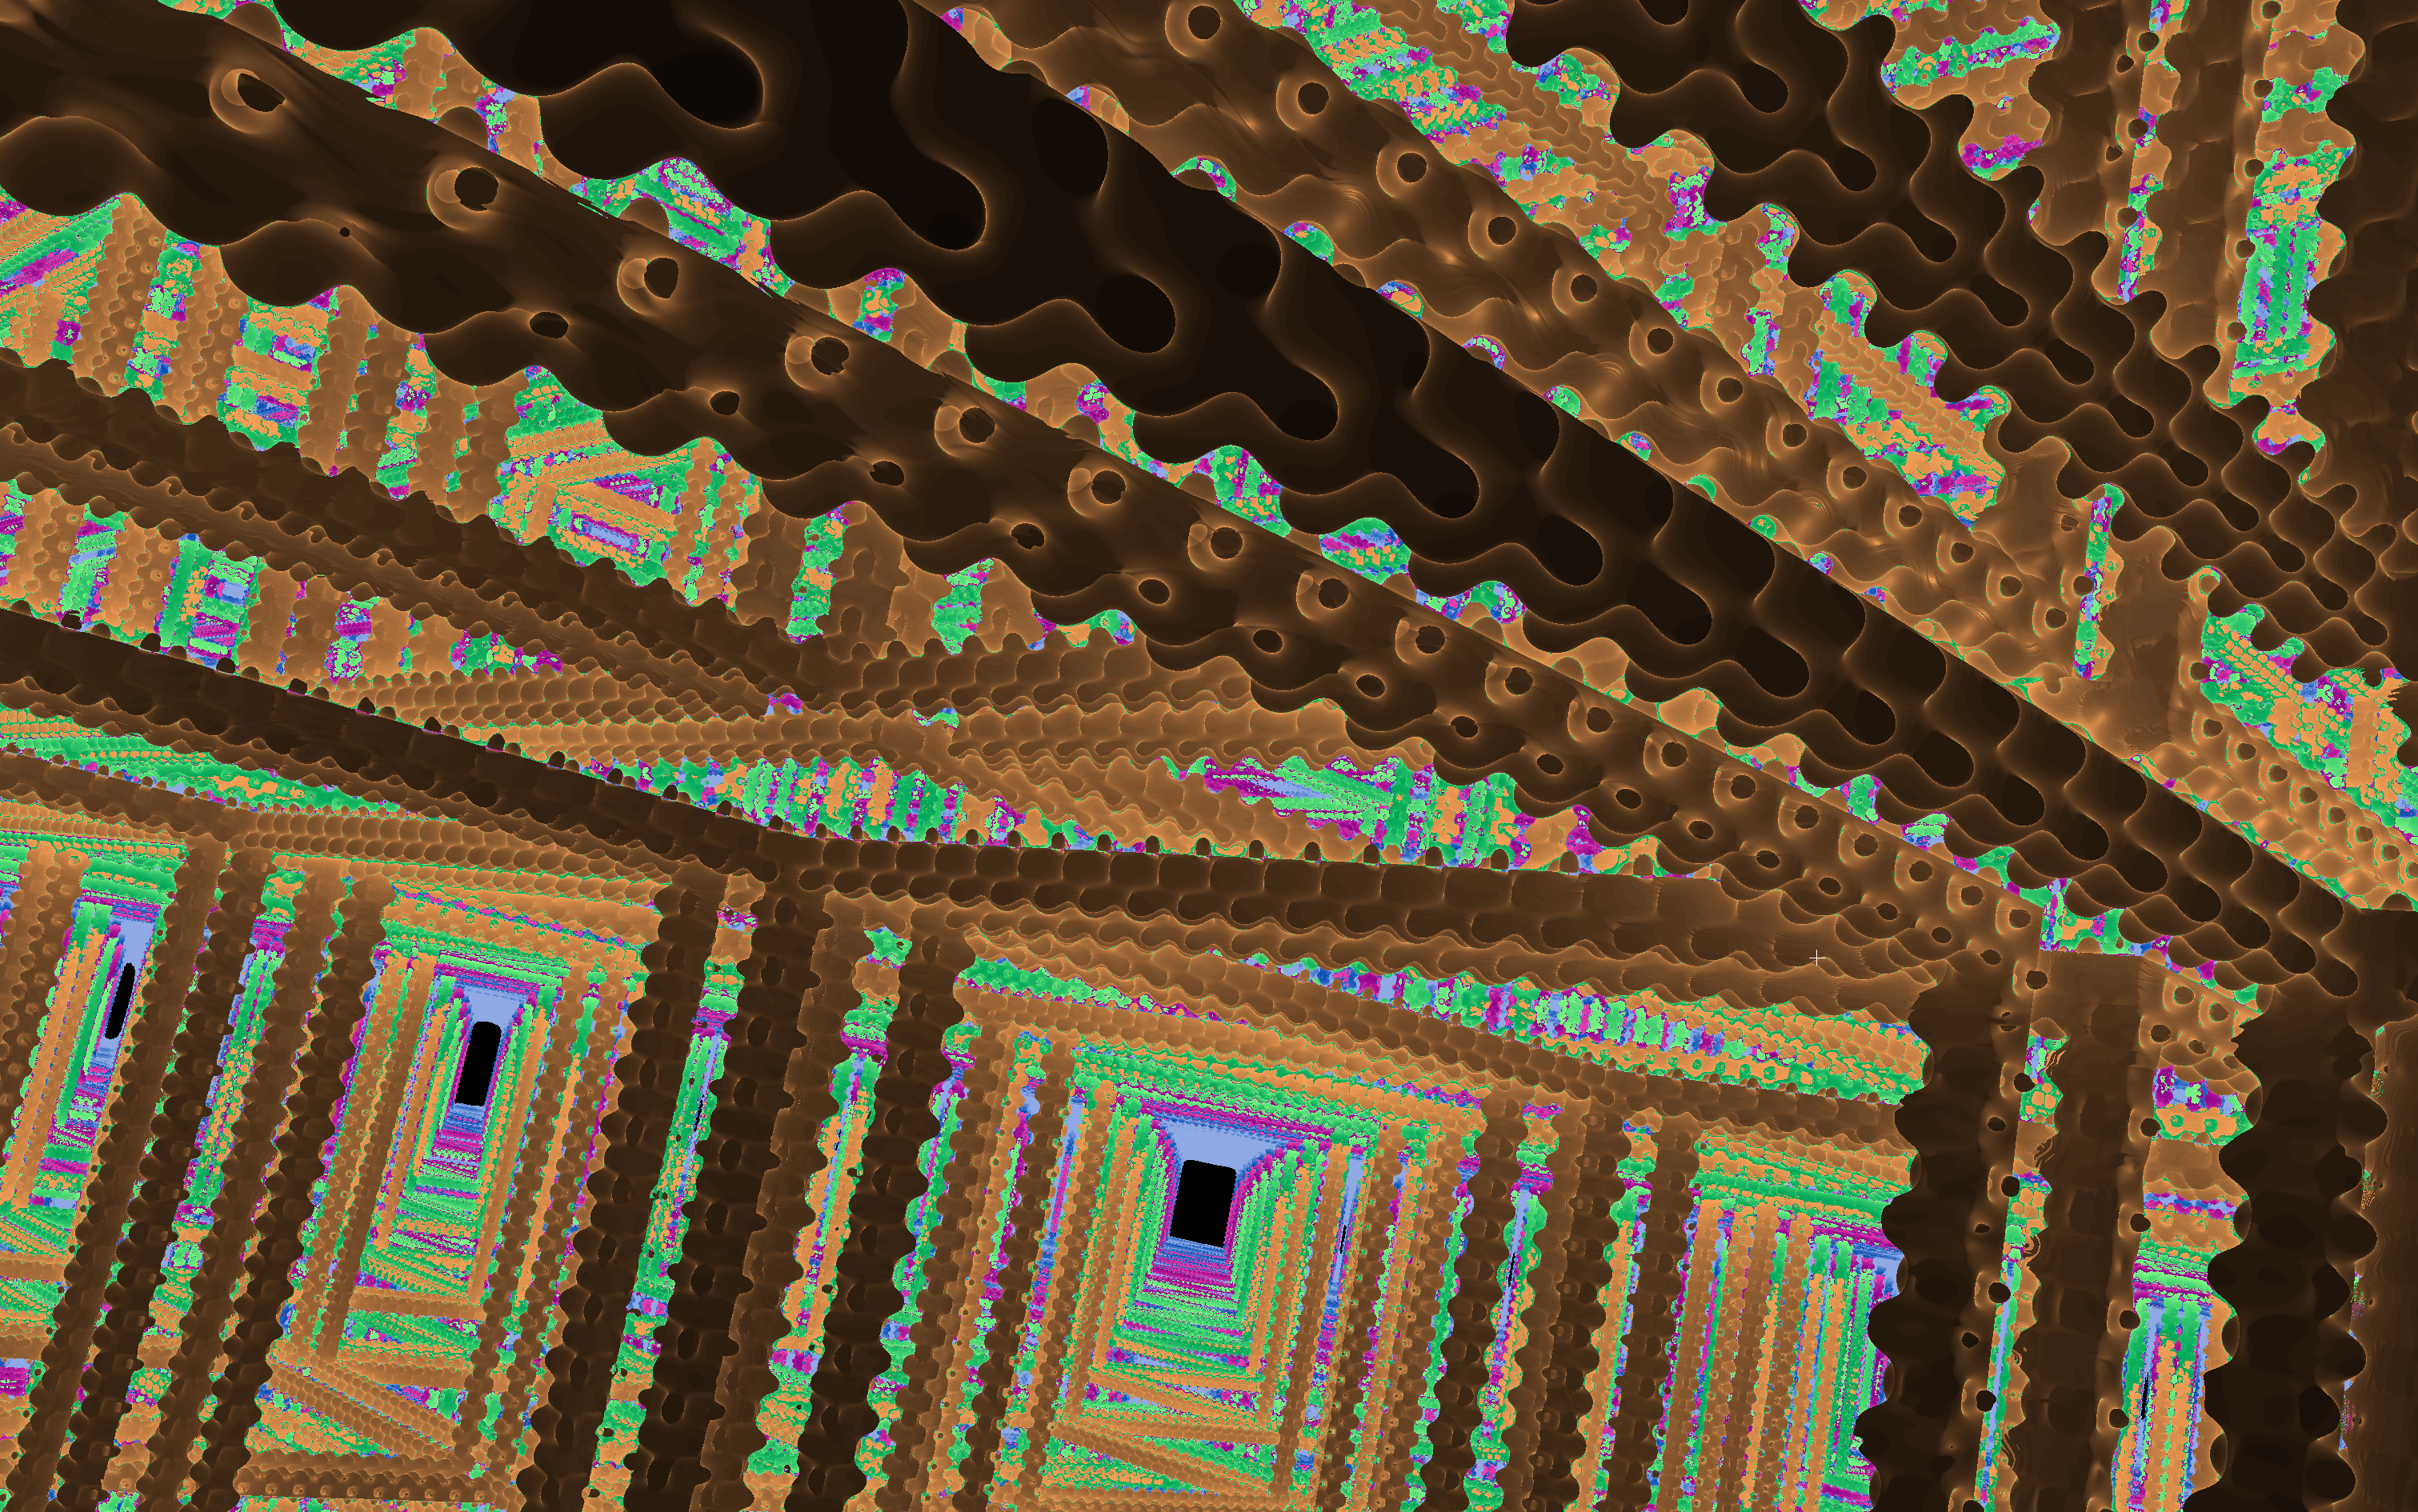
\includegraphics[width=\textwidth,height=0.28\textheight,keepaspectratio]{imgs/AppendixA/render_scaffold_glsl_ceiling.png}
    \caption{GLSL scaffold ceiling close-up. Honeycomb-textured surface on the box-frame boundary under ambient light.}
\end{subfigure}

\vfill

\begin{subfigure}[b]{0.48\textwidth}
    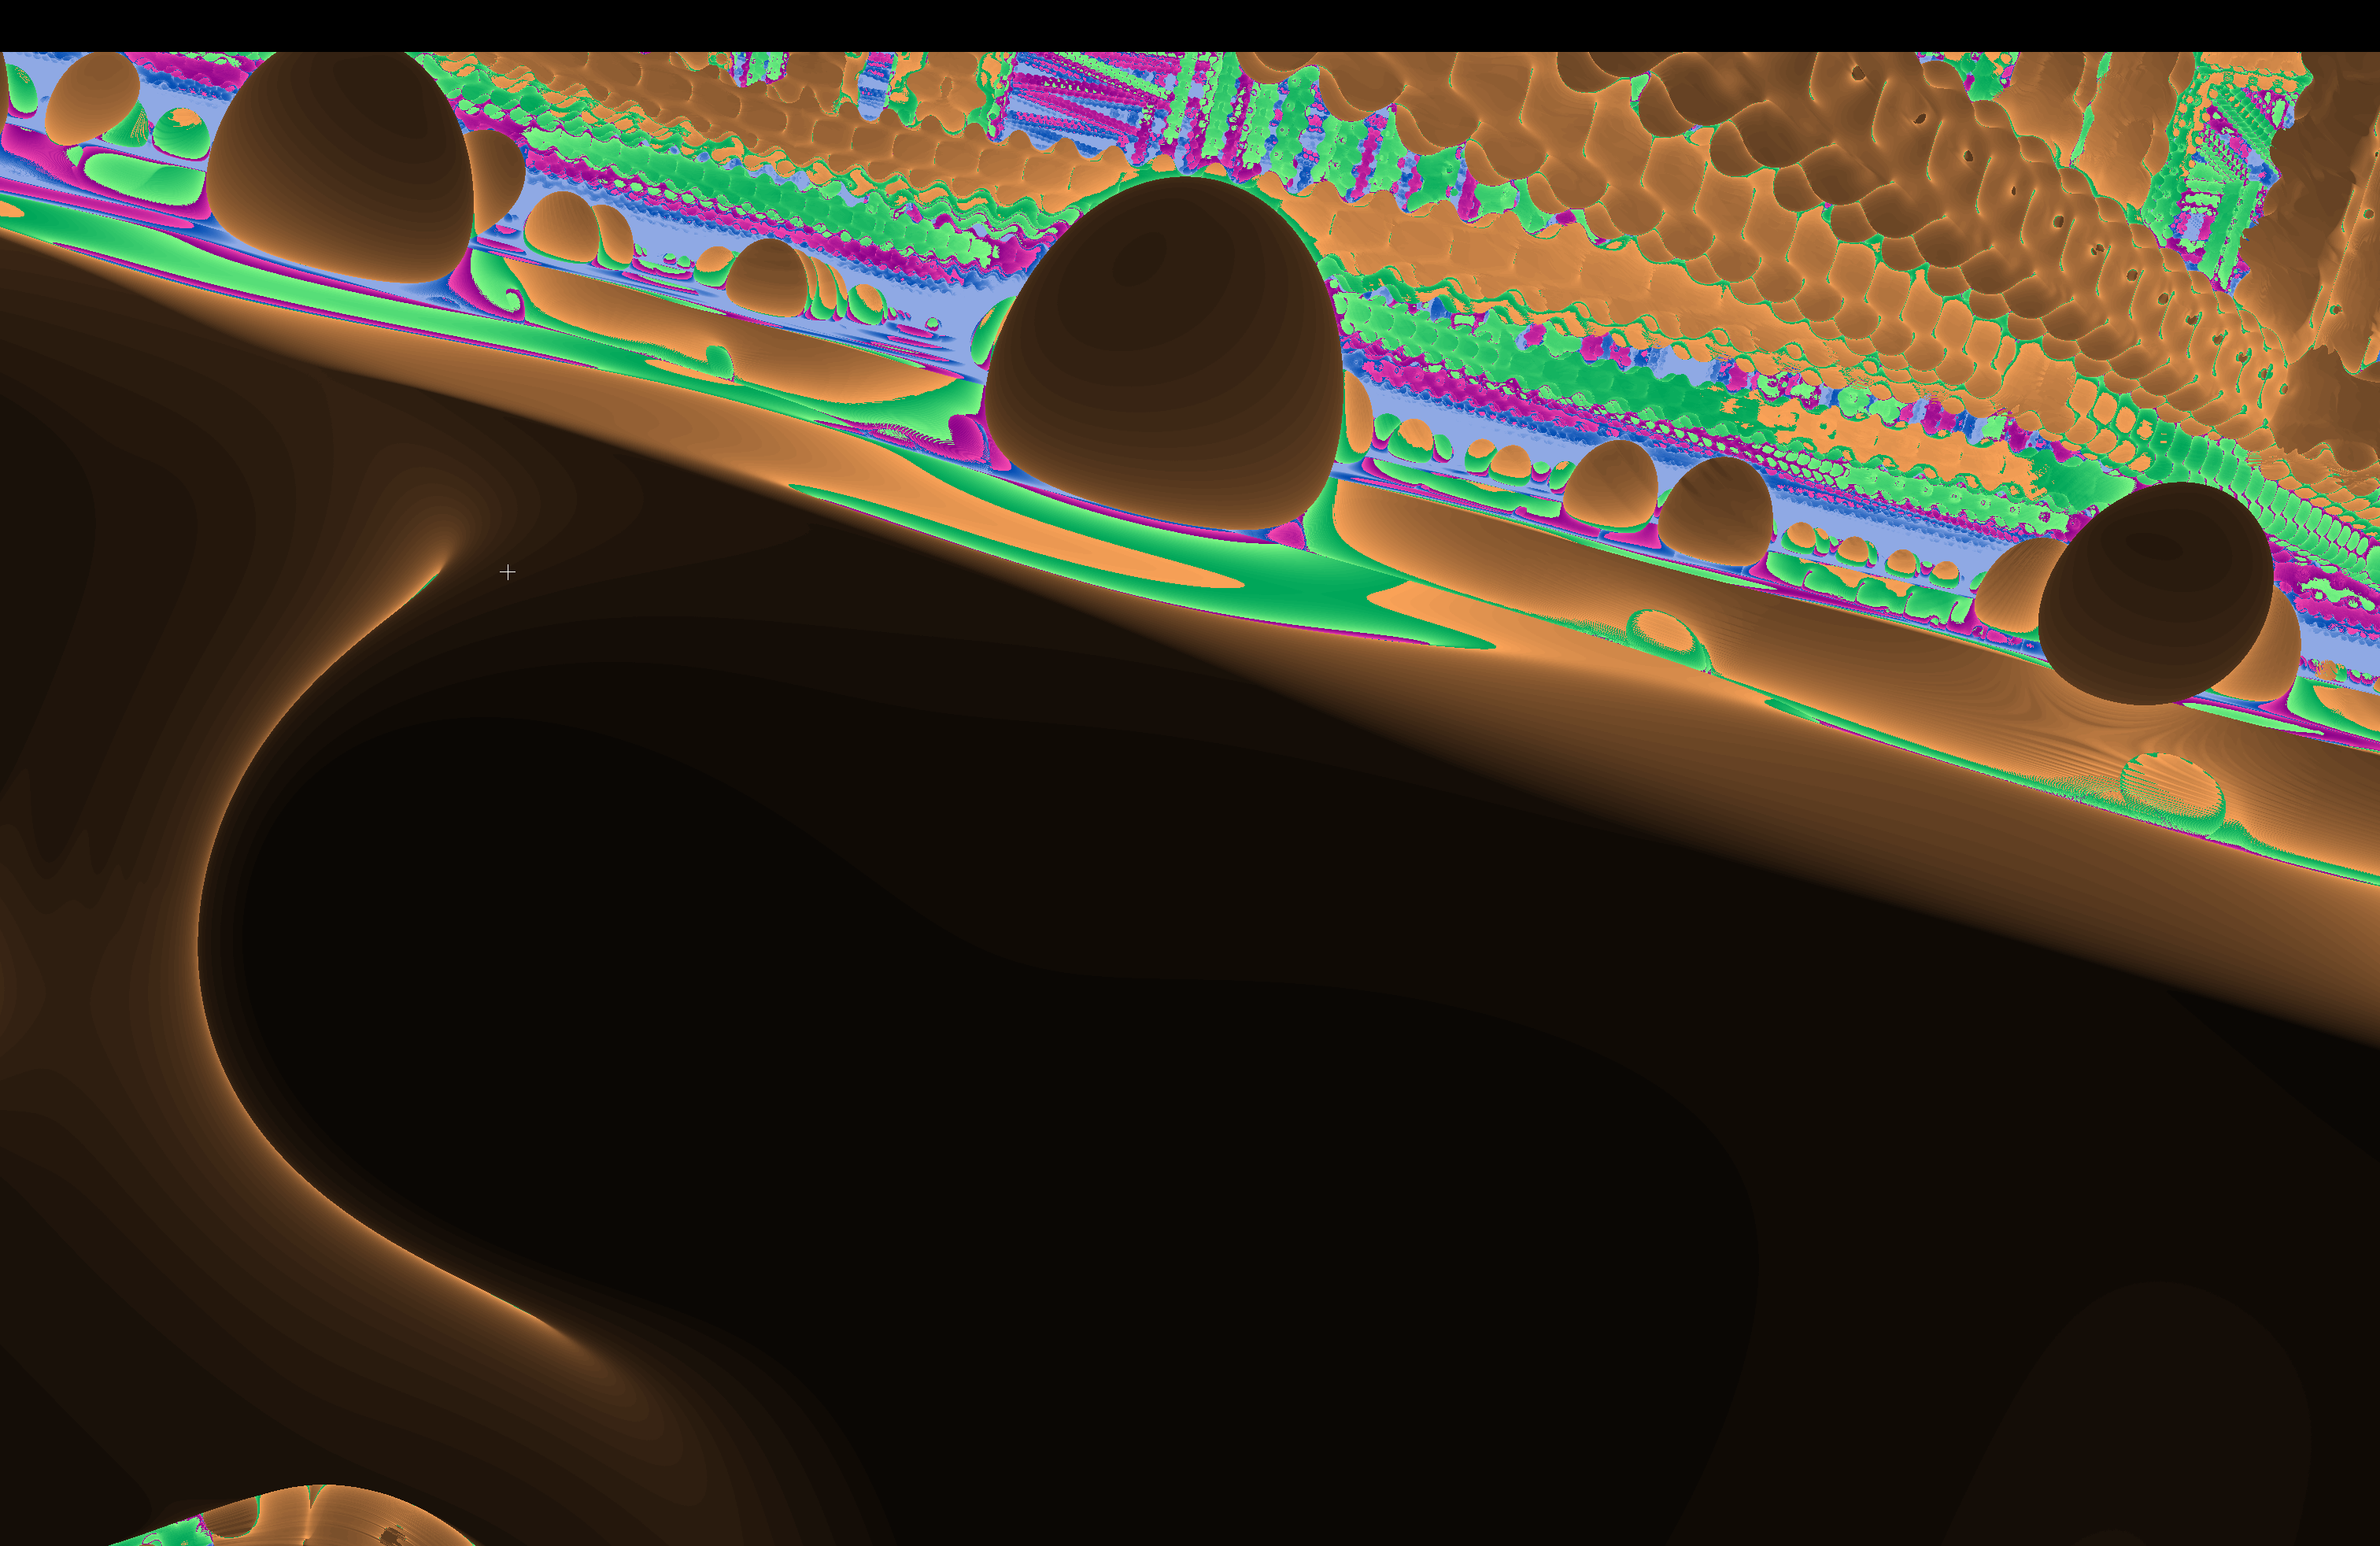
\includegraphics[width=\textwidth,height=0.28\textheight,keepaspectratio]{imgs/AppendixA/render_scaffold_glsl_edge.png}
    \caption{GLSL scaffold exterior edge. Large curved SDF boundary where the sphere-fold meets the scaffold lattice surface.}
\end{subfigure}\hfill
\begin{subfigure}[b]{0.48\textwidth}
    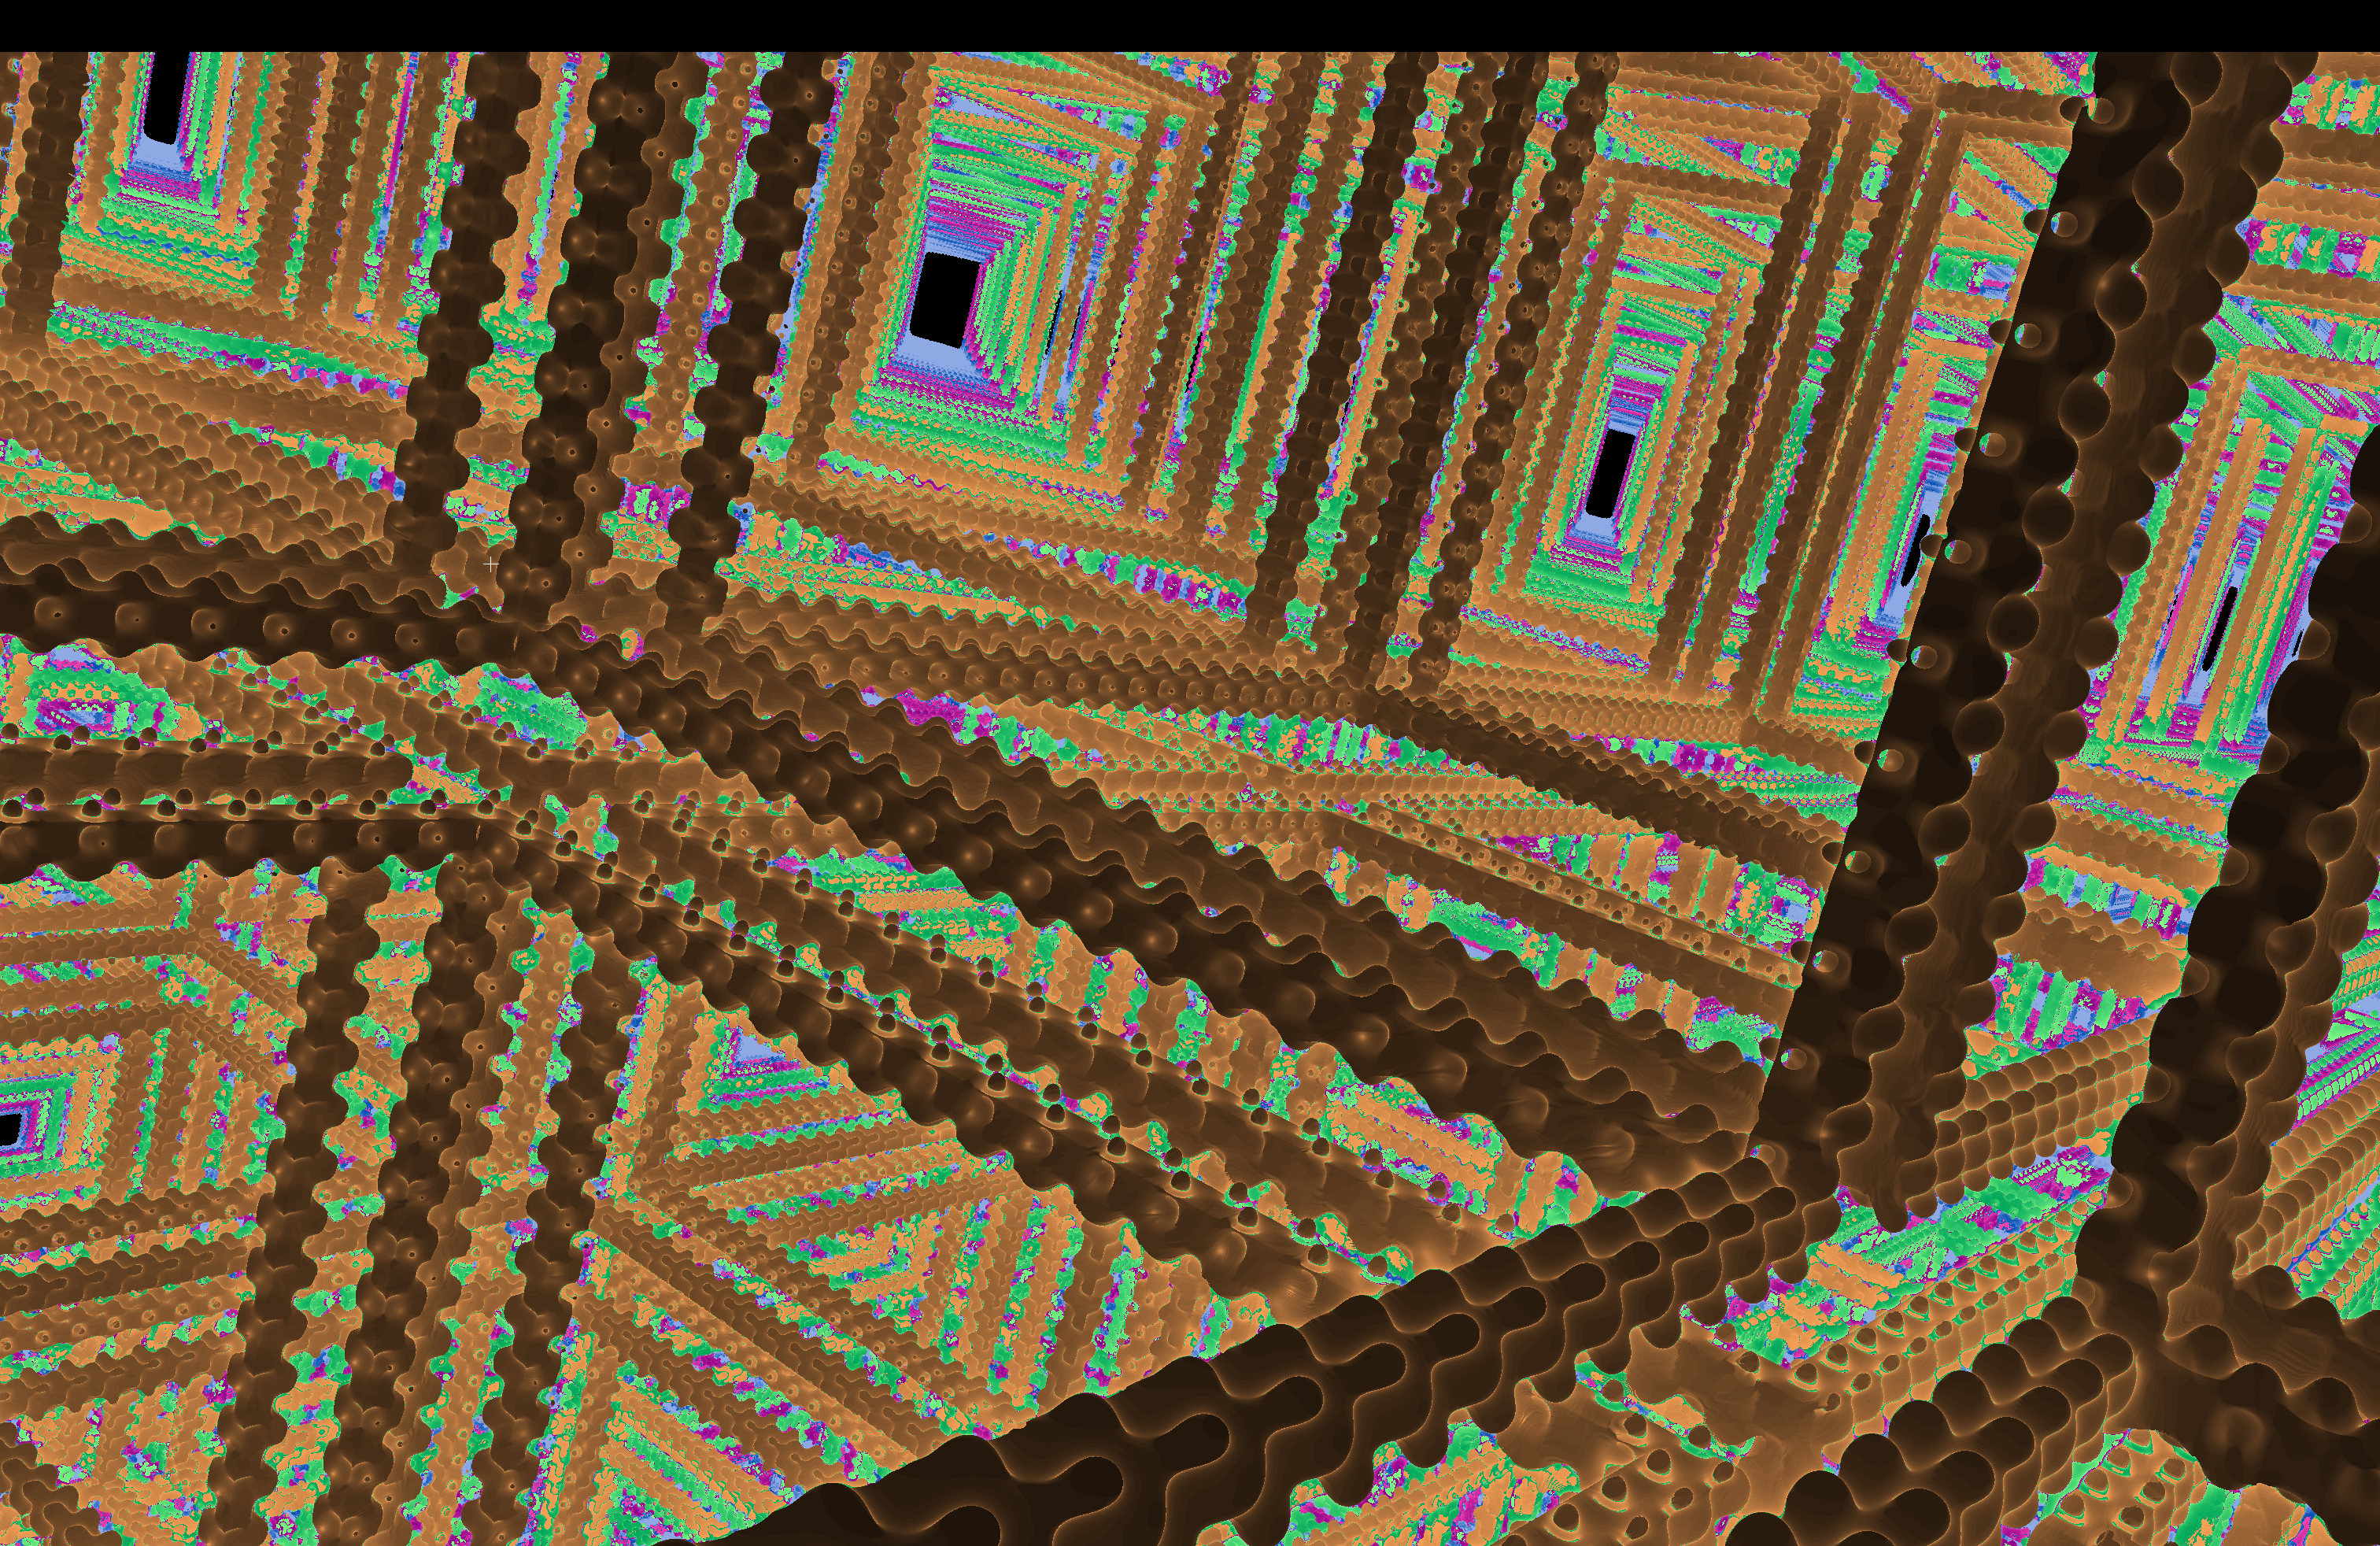
\includegraphics[width=\textwidth,height=0.28\textheight,keepaspectratio]{imgs/AppendixA/render_scaffold_glsl_corner.png}
    \caption{GLSL scaffold corner perspective. Deep lattice recession through frame diagonal; used to validate camera matrix.}
\end{subfigure}

\vfill

\begin{subfigure}[b]{0.48\textwidth}
    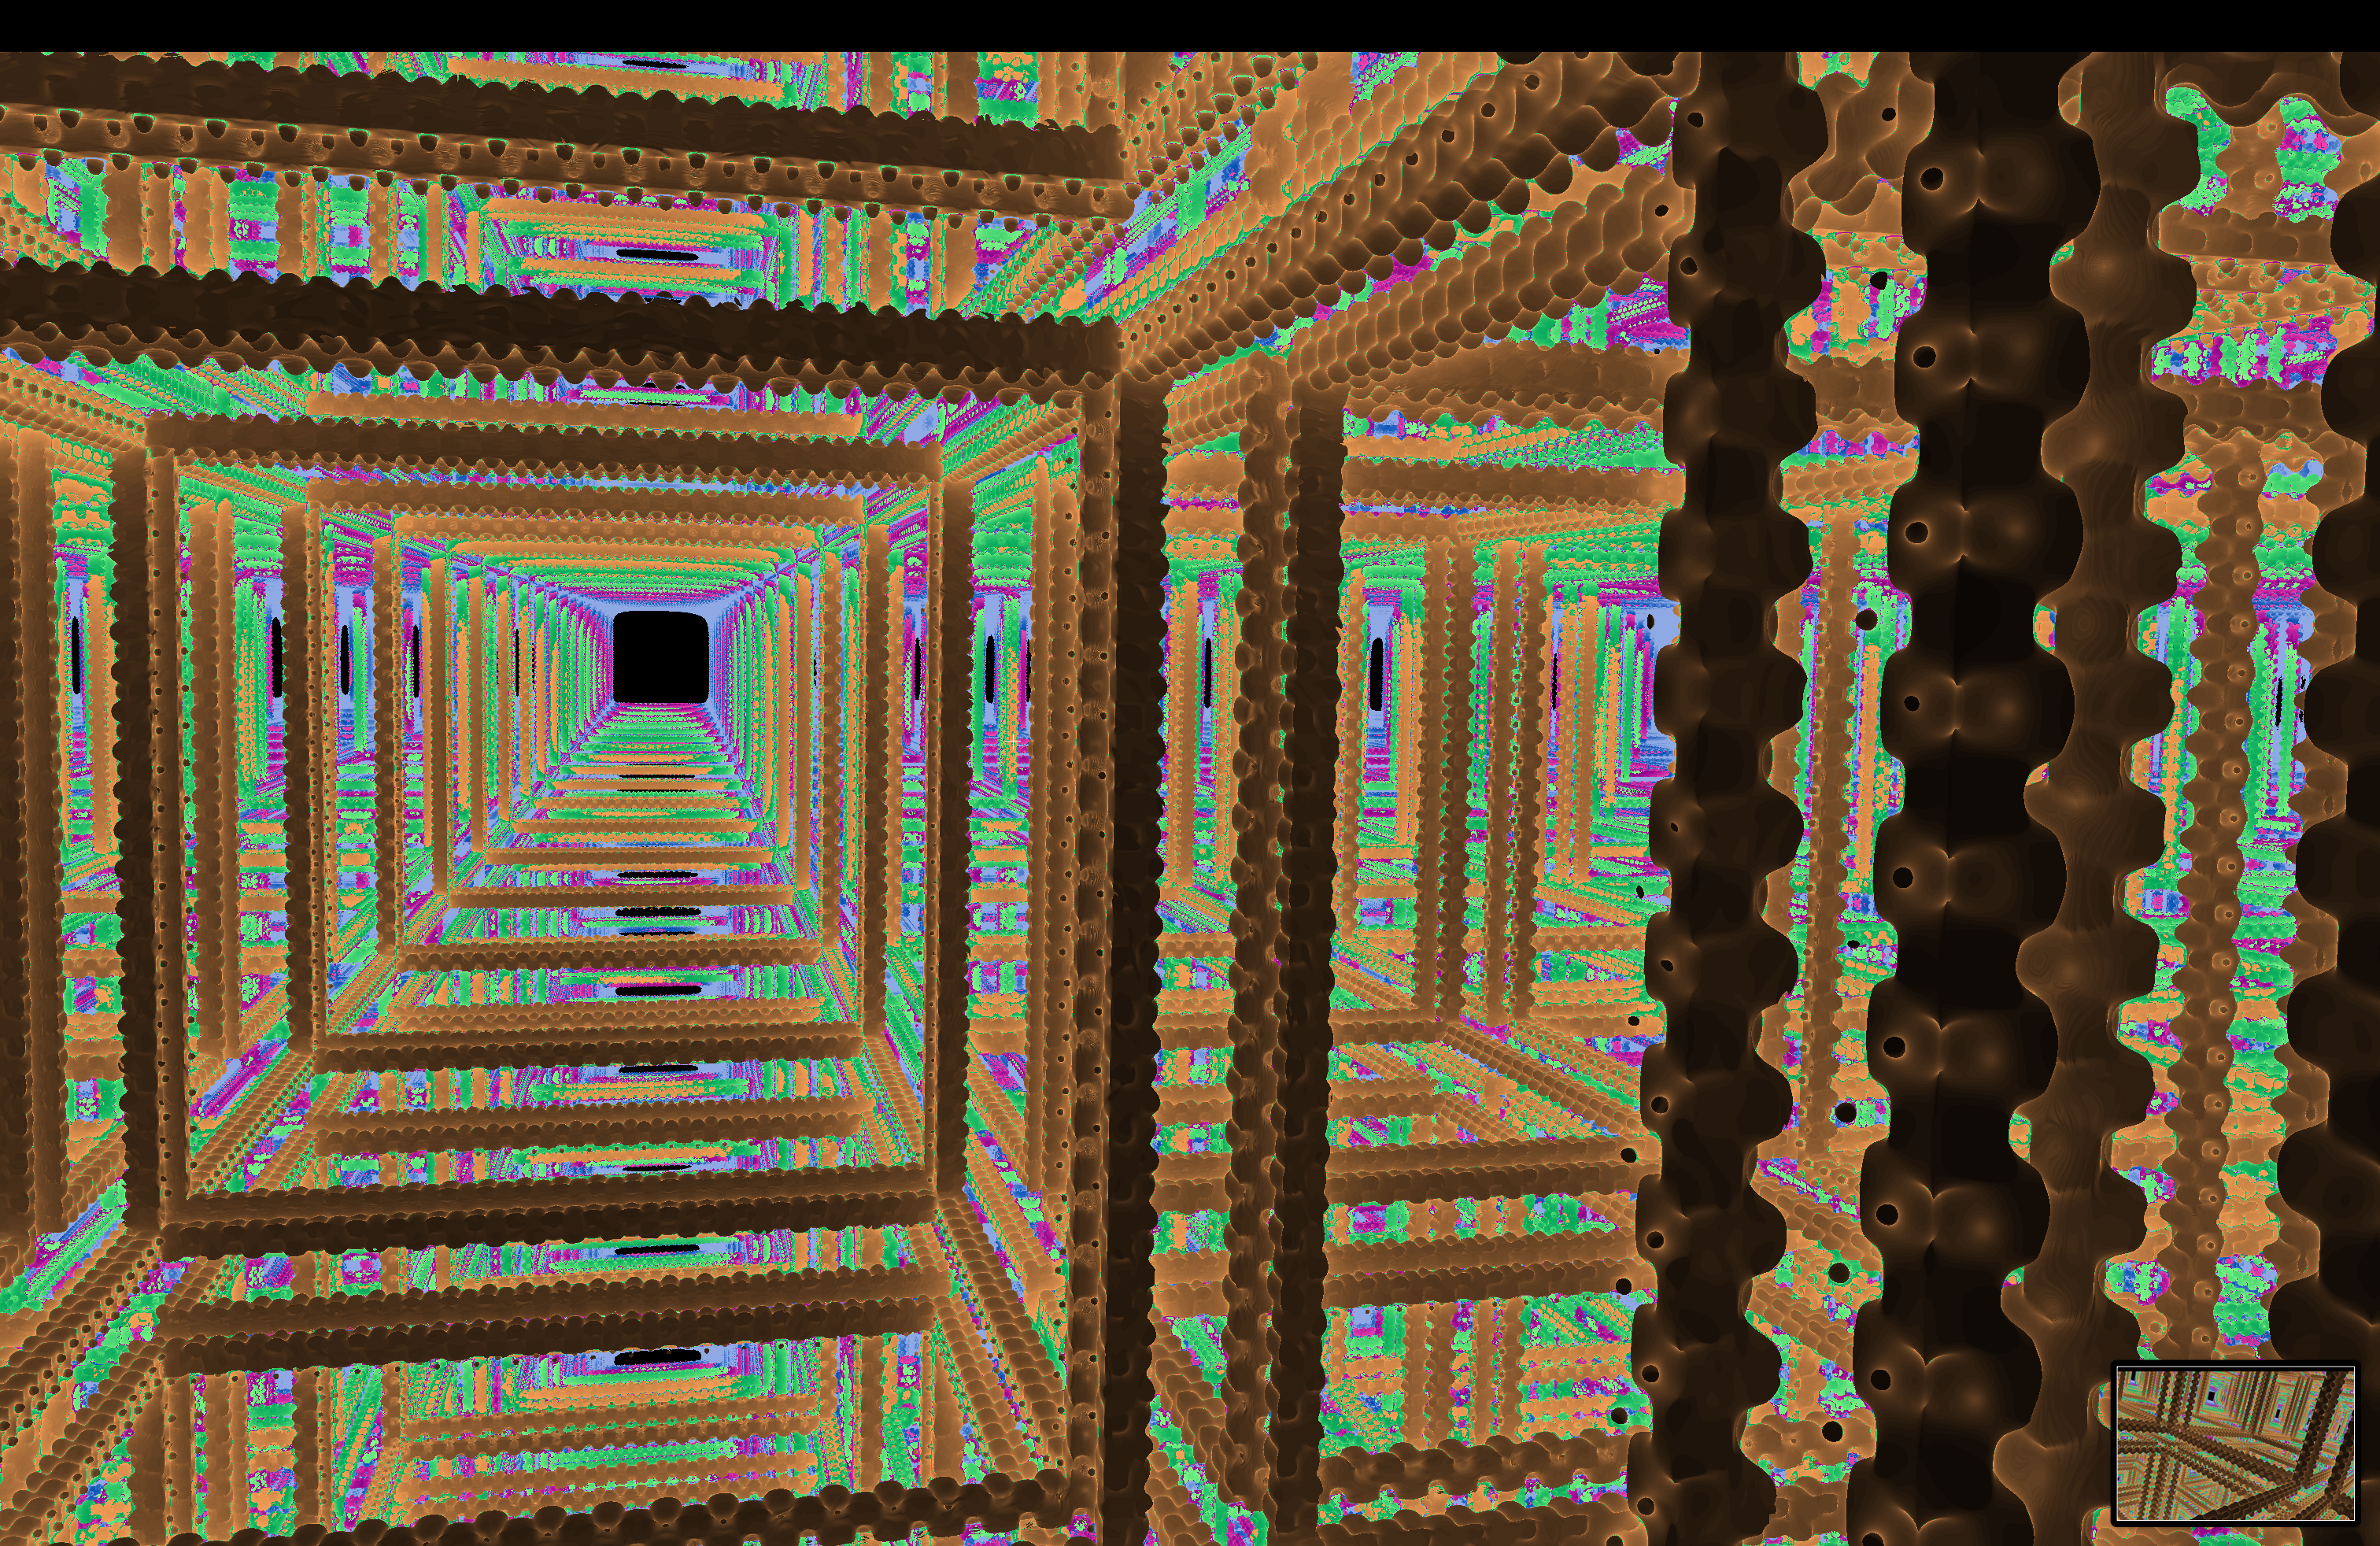
\includegraphics[width=\textwidth,height=0.28\textheight,keepaspectratio]{imgs/AppendixA/render_scaffold_glsl_tunnel.png}
    \caption{GLSL scaffold tunnel with twisted strut column on the right. Used as visual reference for RTL output comparison.}
\end{subfigure}\hfill
\begin{subfigure}[b]{0.48\textwidth}
    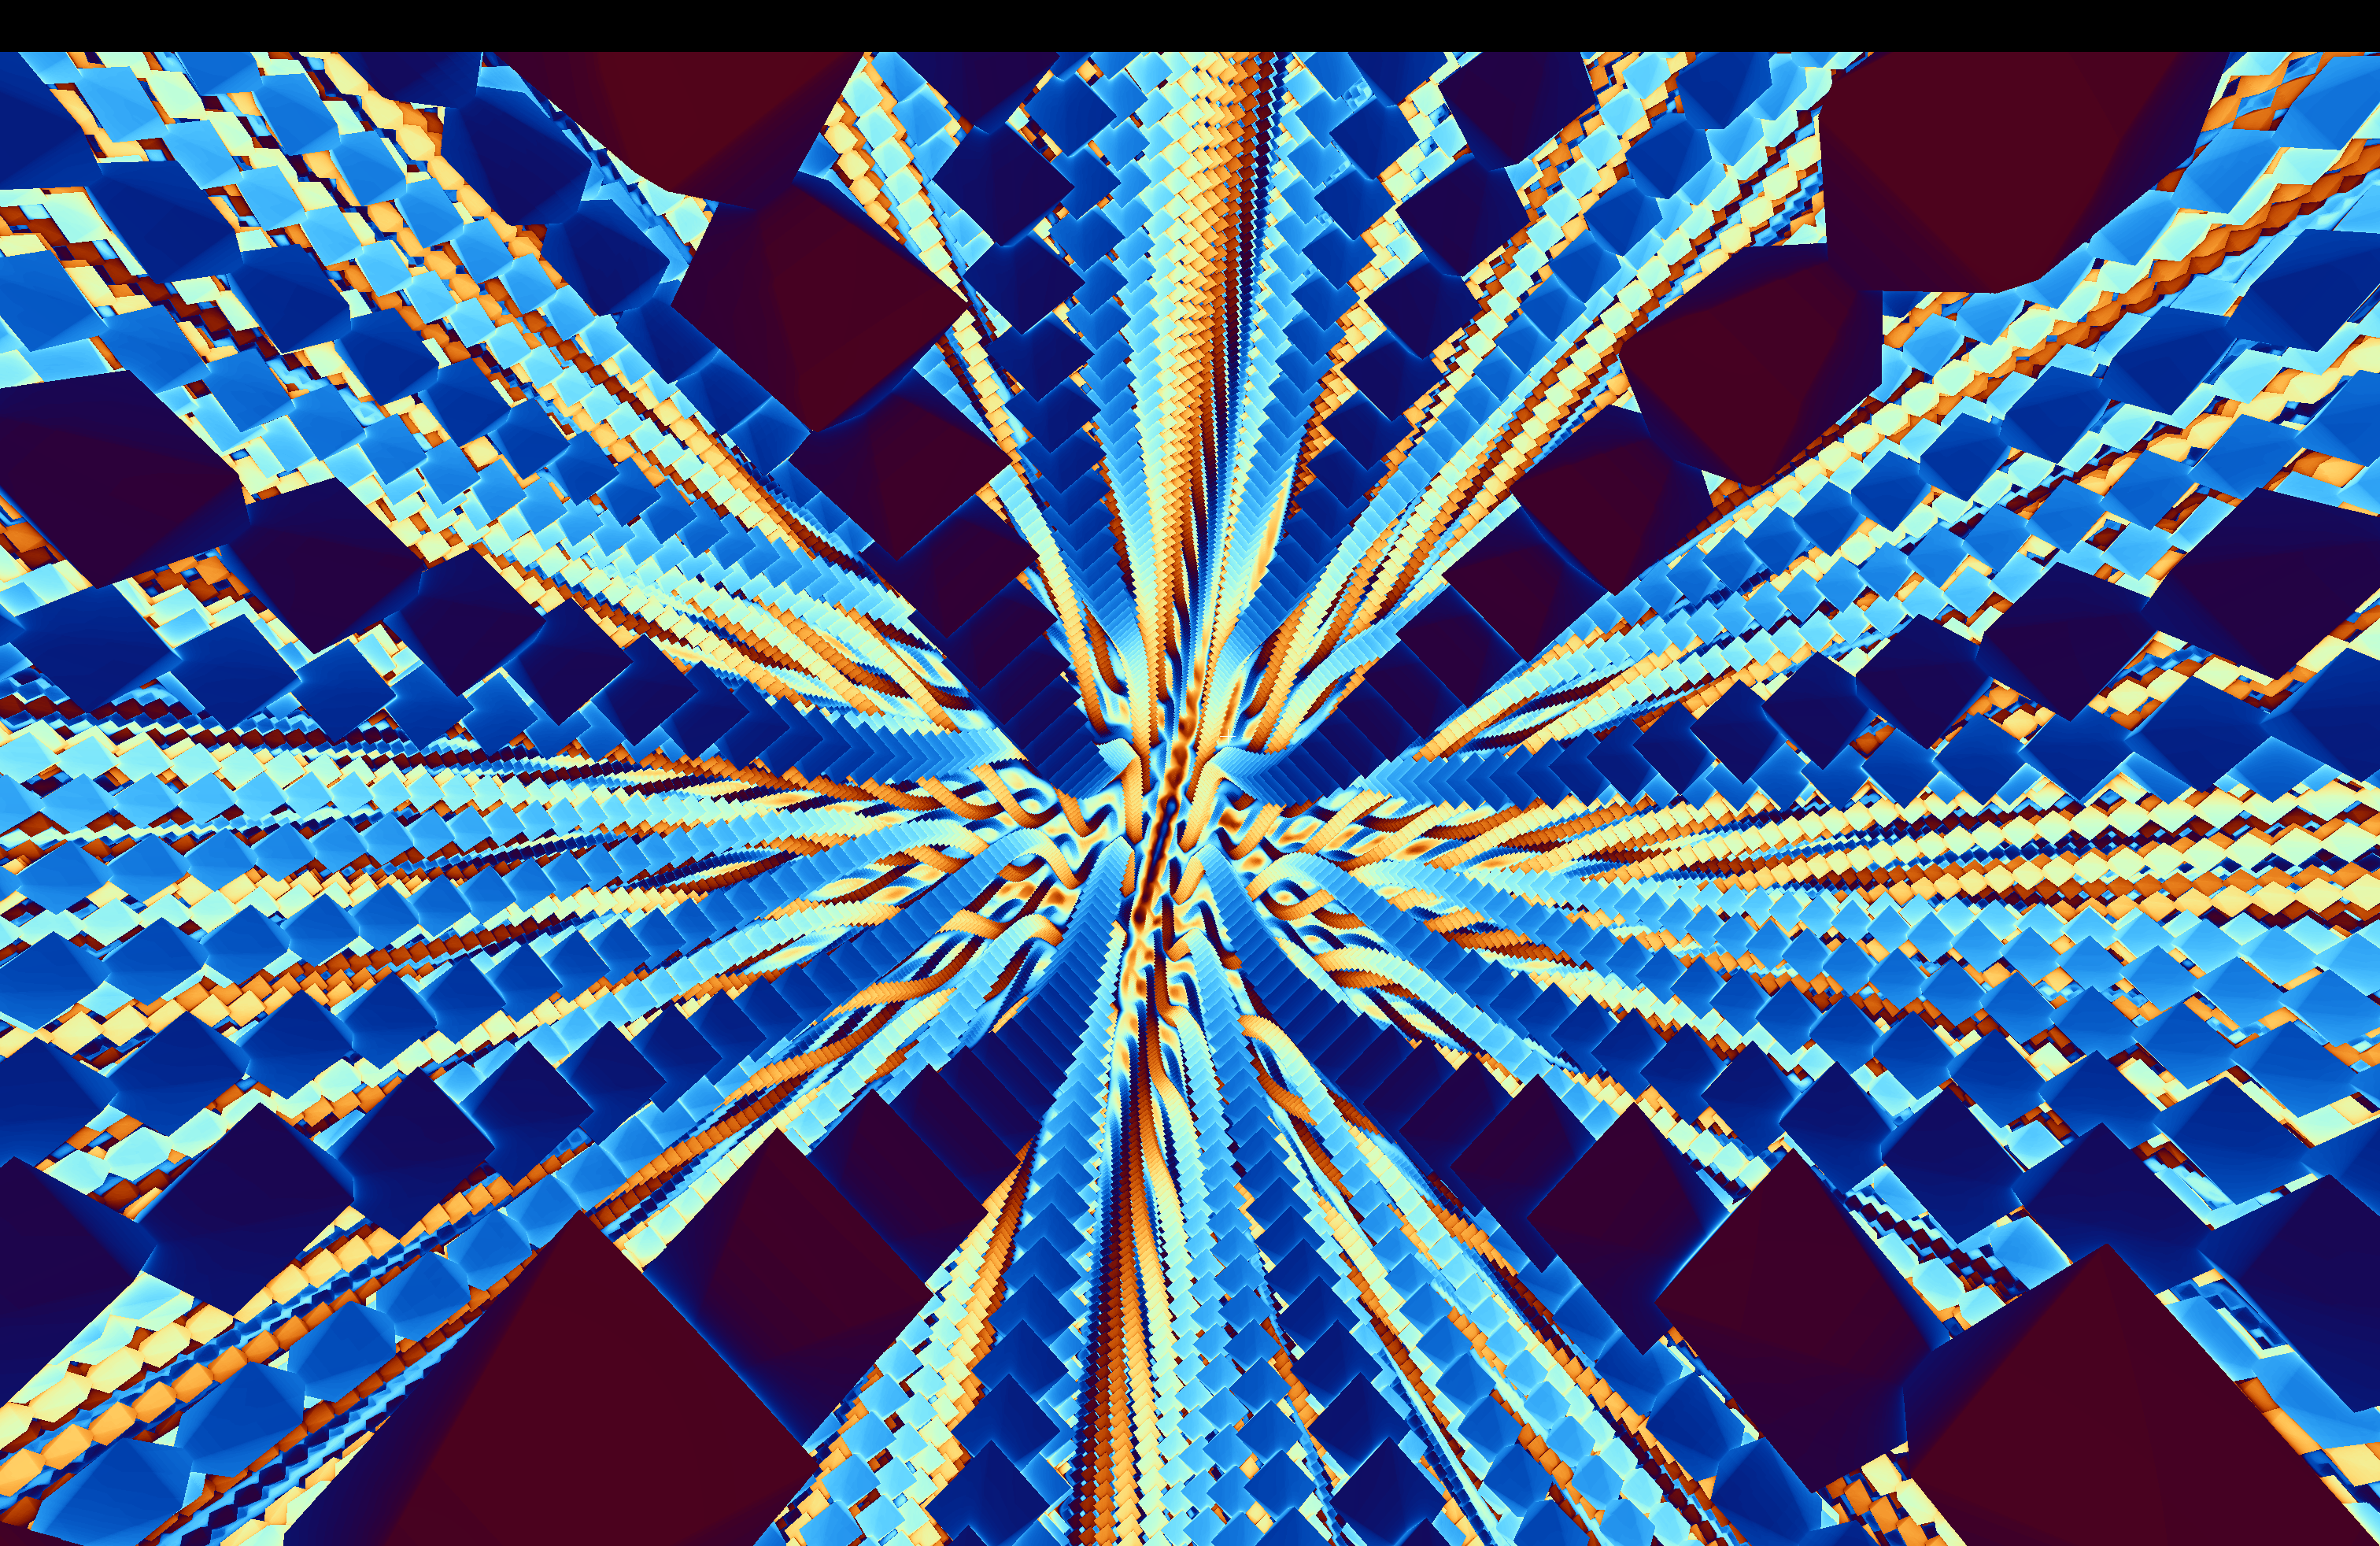
\includegraphics[width=\textwidth,height=0.28\textheight,keepaspectratio]{imgs/AppendixA/render_twisted_torus_glsl_centre.png}
    \caption{Twisted torus SDF in GLSL reference renderer, blue--orange palette, camera aimed at the twist convergence centre.}
\end{subfigure}
\caption{GLSL software reference renders, used for RTL visual verification and camera calibration.}
\end{figure}

\clearpage

% ----------------------------------------------------------------
%  Page 5 — Remaining GLSL renders + VR headset CAD gallery I
% ----------------------------------------------------------------
\begin{figure}[H]
\vspace*{-0.5cm}
\centering
\begin{subfigure}[b]{0.48\textwidth}
    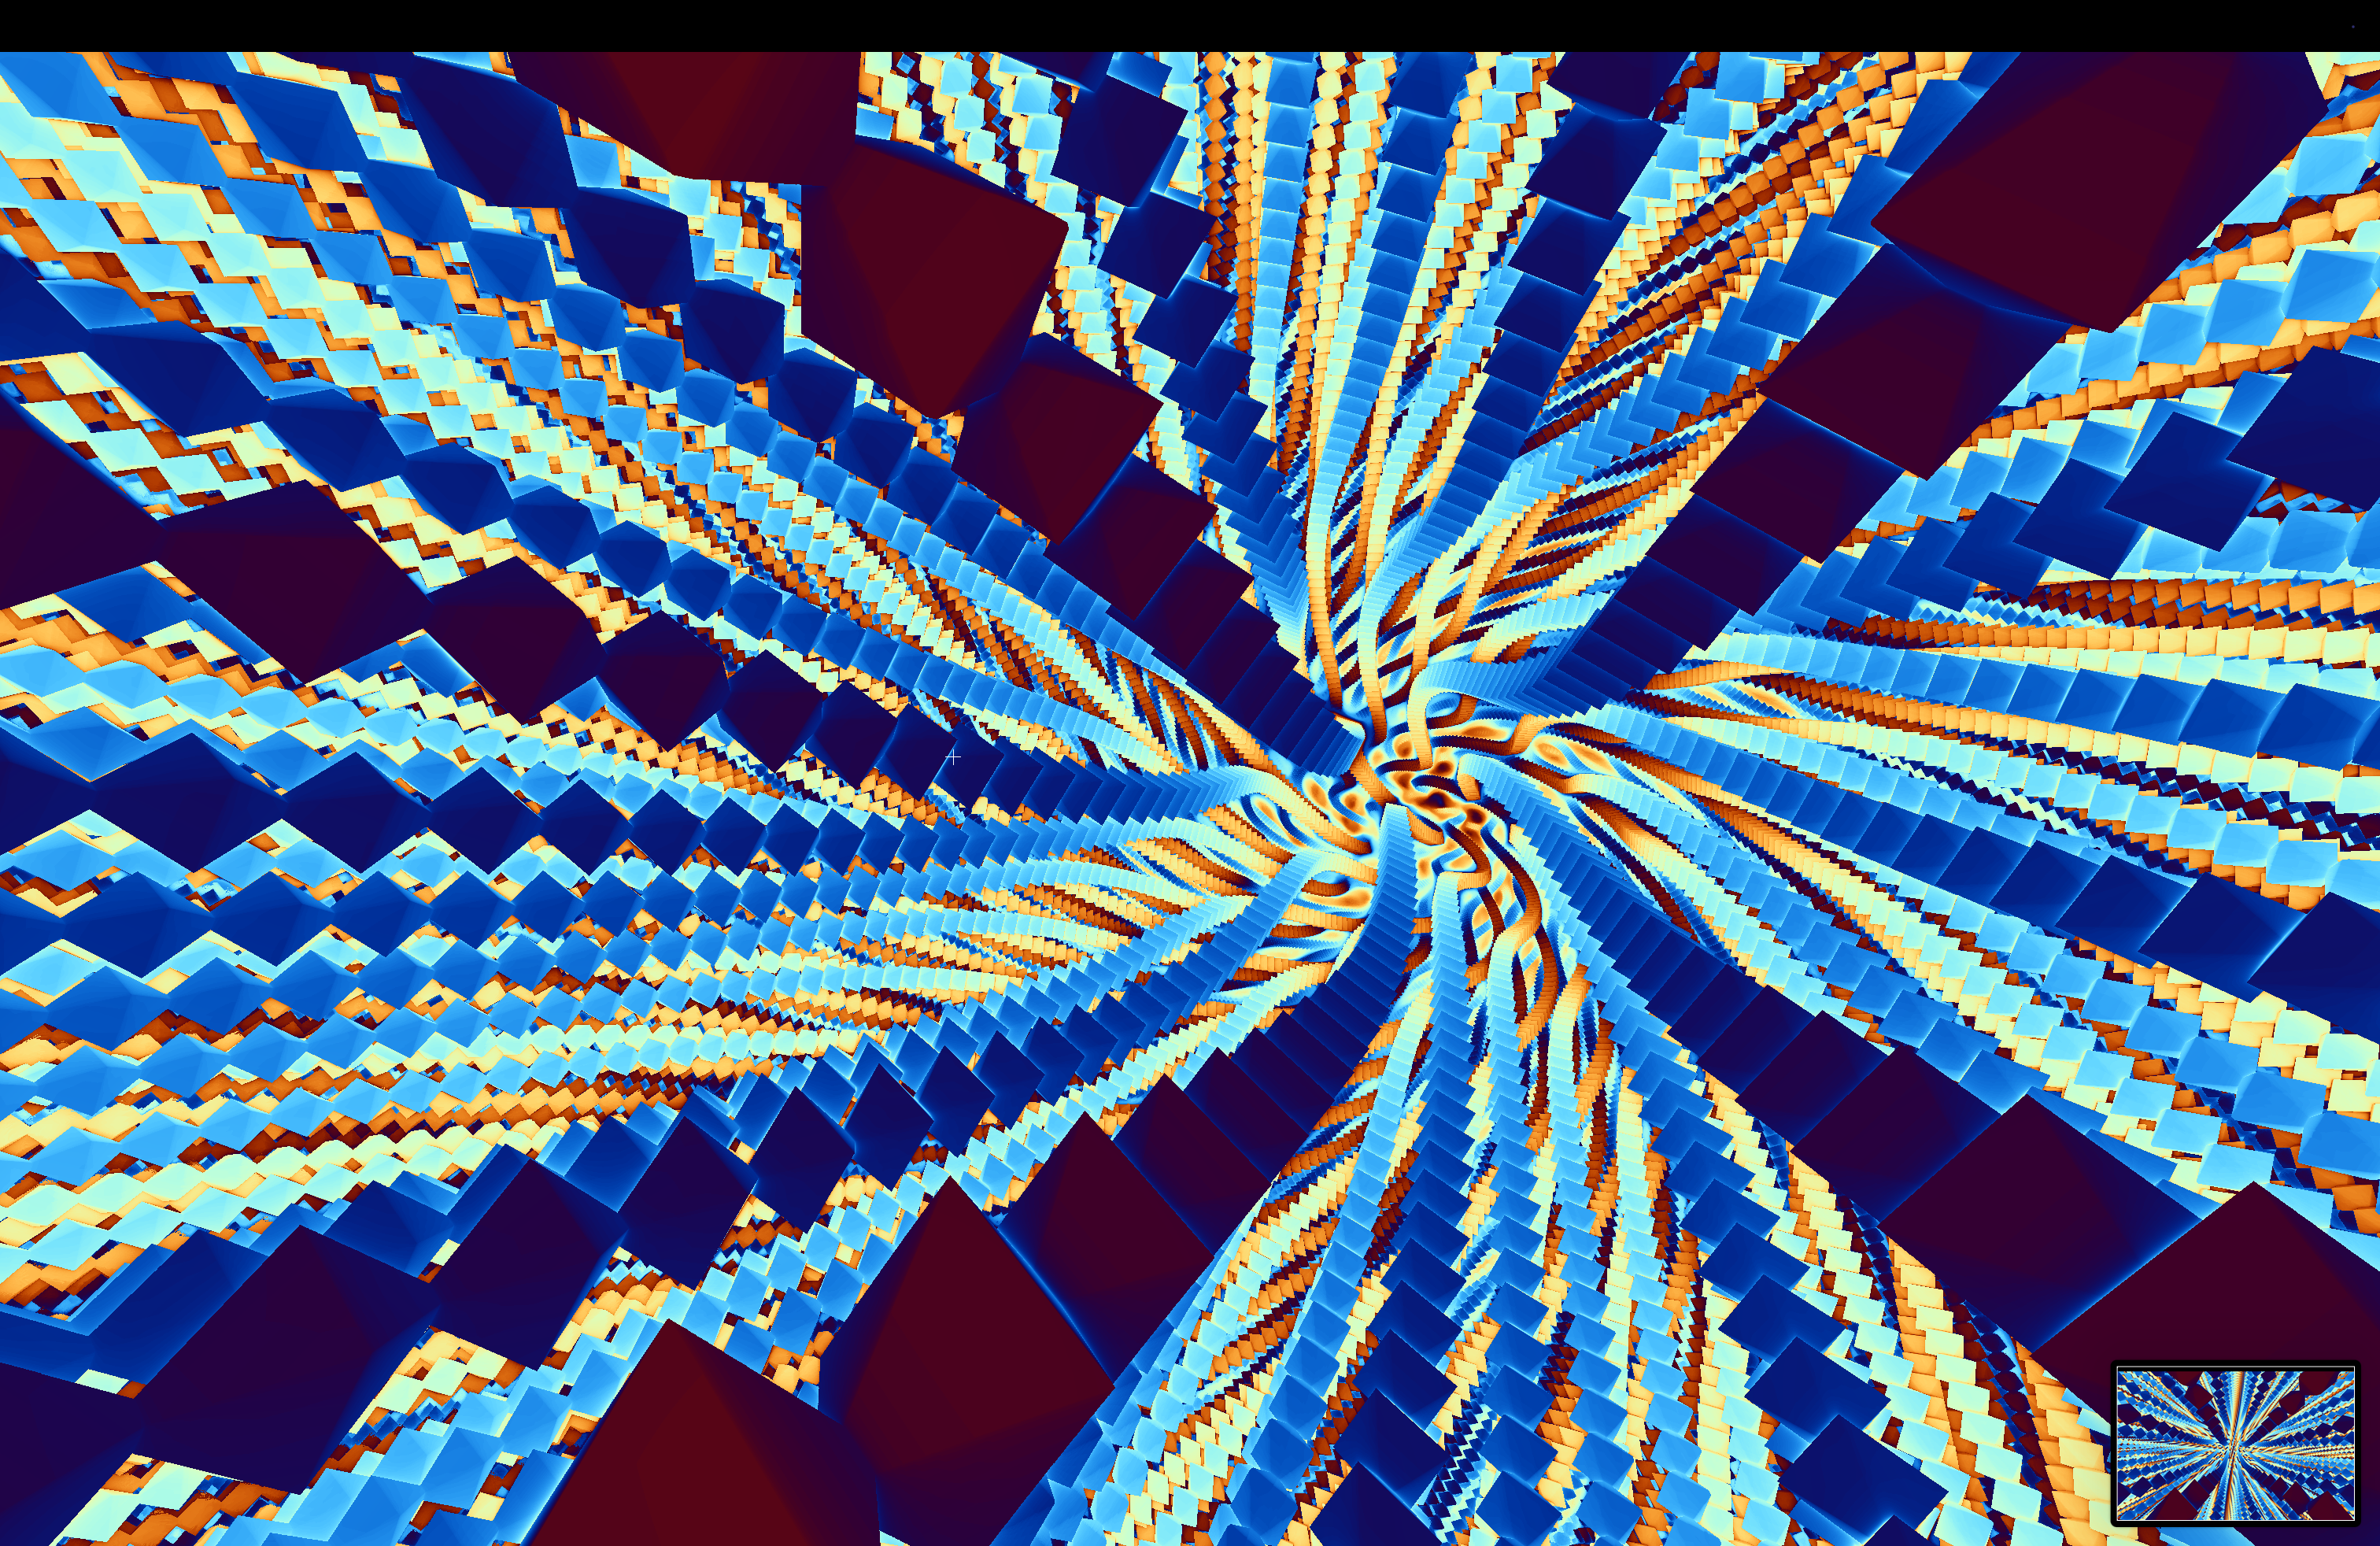
\includegraphics[width=\textwidth,height=0.28\textheight,keepaspectratio]{imgs/AppendixA/render_twisted_torus_glsl_spiral.png}
    \caption{Twisted torus spiral close-up. The twist parameter rotates the torus cross-section continuously around its axis.}
\end{subfigure}\hfill
\begin{subfigure}[b]{0.48\textwidth}
    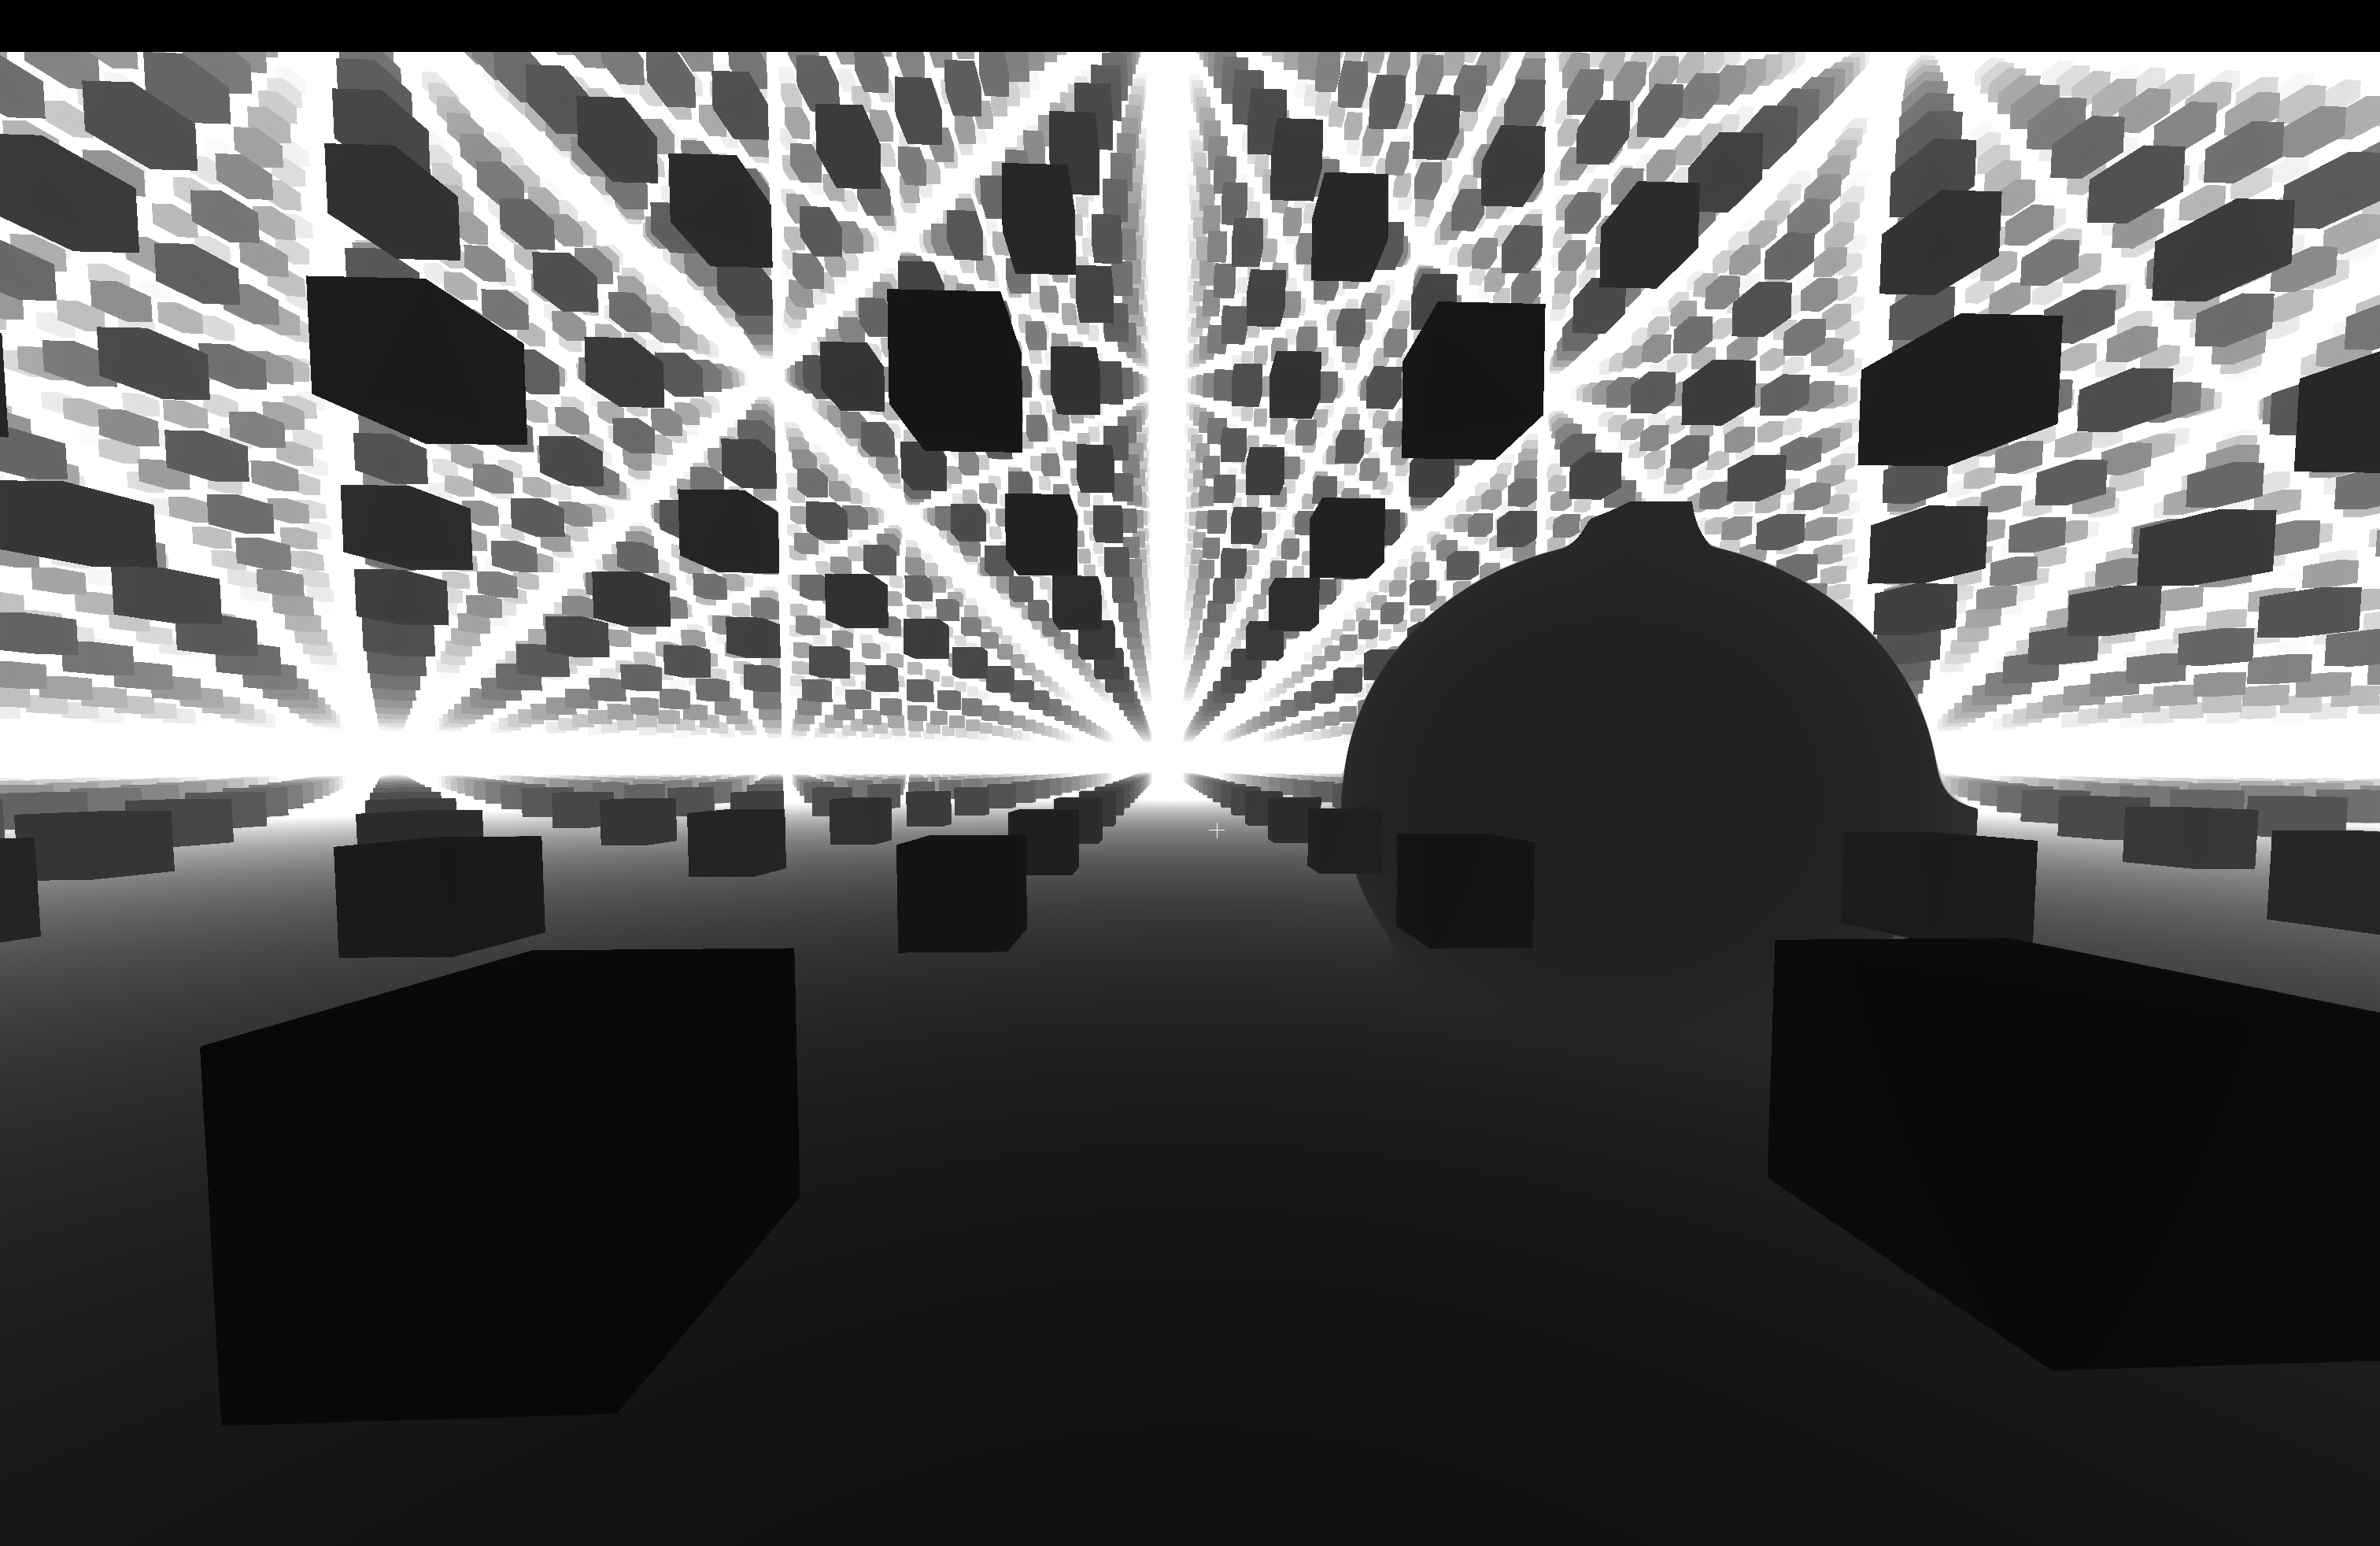
\includegraphics[width=\textwidth,height=0.28\textheight,keepaspectratio]{imgs/AppendixA/render_glsl_boxes_reference.png}
    \caption{GLSL reference scene, black-and-white box primitives on a reflective floor with starburst diffraction pattern.}
\end{subfigure}

\vfill

\begin{subfigure}[b]{0.48\textwidth}
    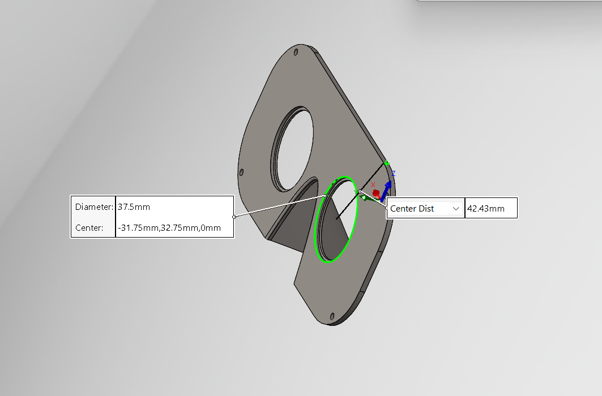
\includegraphics[width=\textwidth,height=0.28\textheight,keepaspectratio]{imgs/Headset_Images/lens_mount.png}
    \caption{Lens cup friction-fit CAD. 37\,mm biconvex lens diameter toleranced to $+0.5$\,mm for tool-free insertion.}
\end{subfigure}\hfill
\begin{subfigure}[b]{0.48\textwidth}
    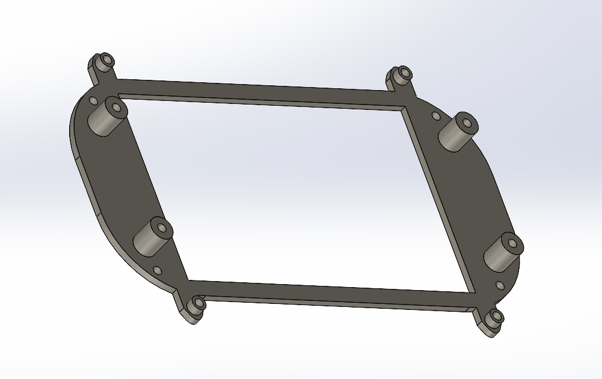
\includegraphics[width=\textwidth,height=0.28\textheight,keepaspectratio]{imgs/Headset_Images/screen_panel.png}
    \caption{Screen panel redesign. Entire panel rebuilt from scratch to achieve exact 45\,mm focal length for the 5-inch LCD.}
\end{subfigure}

\vfill

\begin{subfigure}[b]{0.48\textwidth}
    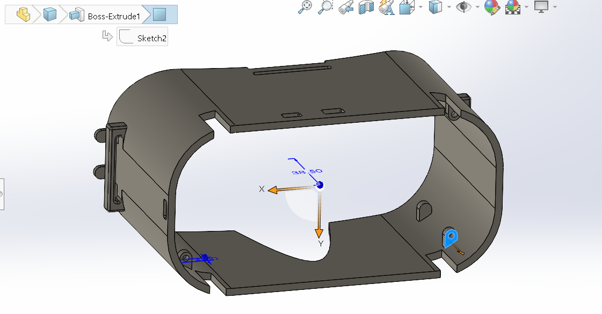
\includegraphics[width=\textwidth,height=0.28\textheight,keepaspectratio]{imgs/Headset_Images/body.png}
    \caption{Headset chassis body after focal-length depth adjustments. Extended body accommodates FPGA housing at the front.}
\end{subfigure}\hfill
\begin{subfigure}[b]{0.48\textwidth}
    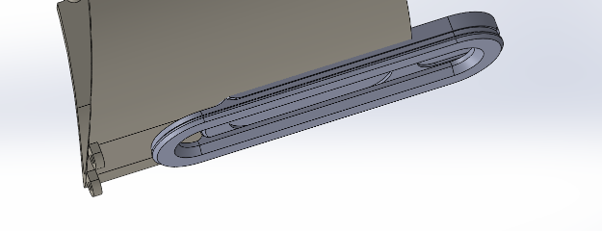
\includegraphics[width=\textwidth,height=0.28\textheight,keepaspectratio]{imgs/Headset_Images/quest2_strap_1.png}
    \caption{Quest~2 headstrap adapter arm, first image. Original velcro slot removed; adapter mated forward to clear screw holes.}
\end{subfigure}
\caption{GLSL reference renders continued and VR headset CAD gallery I.}
\end{figure}

\clearpage

% ----------------------------------------------------------------
%  Page 6 — VR headset CAD gallery II + system diagrams
% ----------------------------------------------------------------
\begin{figure}[H]
\vspace*{-0.5cm}
\centering
\begin{subfigure}[b]{0.48\textwidth}
    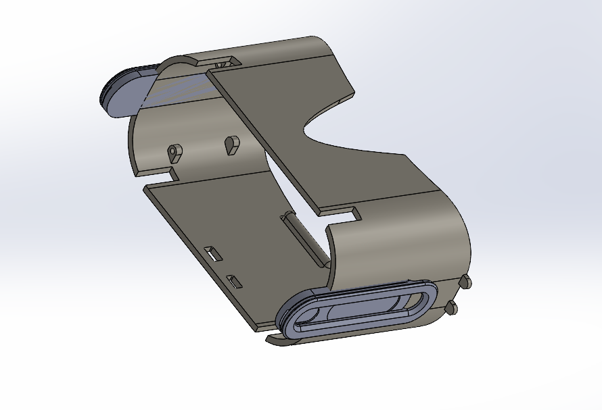
\includegraphics[width=\textwidth,height=0.28\textheight,keepaspectratio]{imgs/Headset_Images/quest2_strap_2.png}
    \caption{Quest~2 headstrap adapter arm, second image. Quest~3 geometry removed; Quest~2 clip mated directly to body.}
\end{subfigure}\hfill
\begin{subfigure}[b]{0.48\textwidth}
    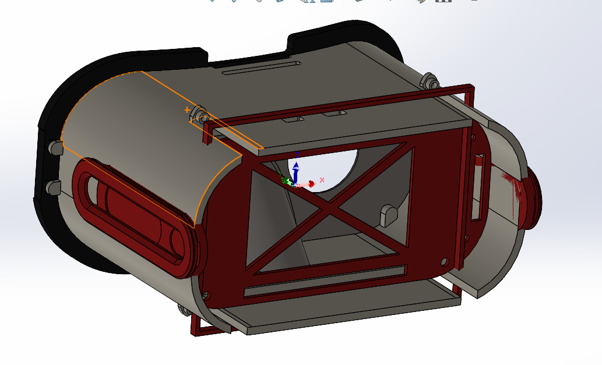
\includegraphics[width=\textwidth,height=0.28\textheight,keepaspectratio]{imgs/Headset_Images/fpga_housing_1.png}
    \caption{FPGA housing cavity. Internal dimensions set at $+0.5$--$1$\,mm tolerance for a tool-free friction fit of the PYNQ case.}
\end{subfigure}

\vfill

\begin{subfigure}[b]{0.48\textwidth}
    
\includegraphics[width=\textwidth,height=0.28\textheight,keepaspectratio]{imgs/Headset_Images/most_front_panel.png}
    \caption{Front panel with IMU mounting bracket and 4\,mm standoffs ensuring the MPU-6050 sits level for accurate tracking.}
\end{subfigure}\hfill
\begin{subfigure}[b]{0.48\textwidth}
    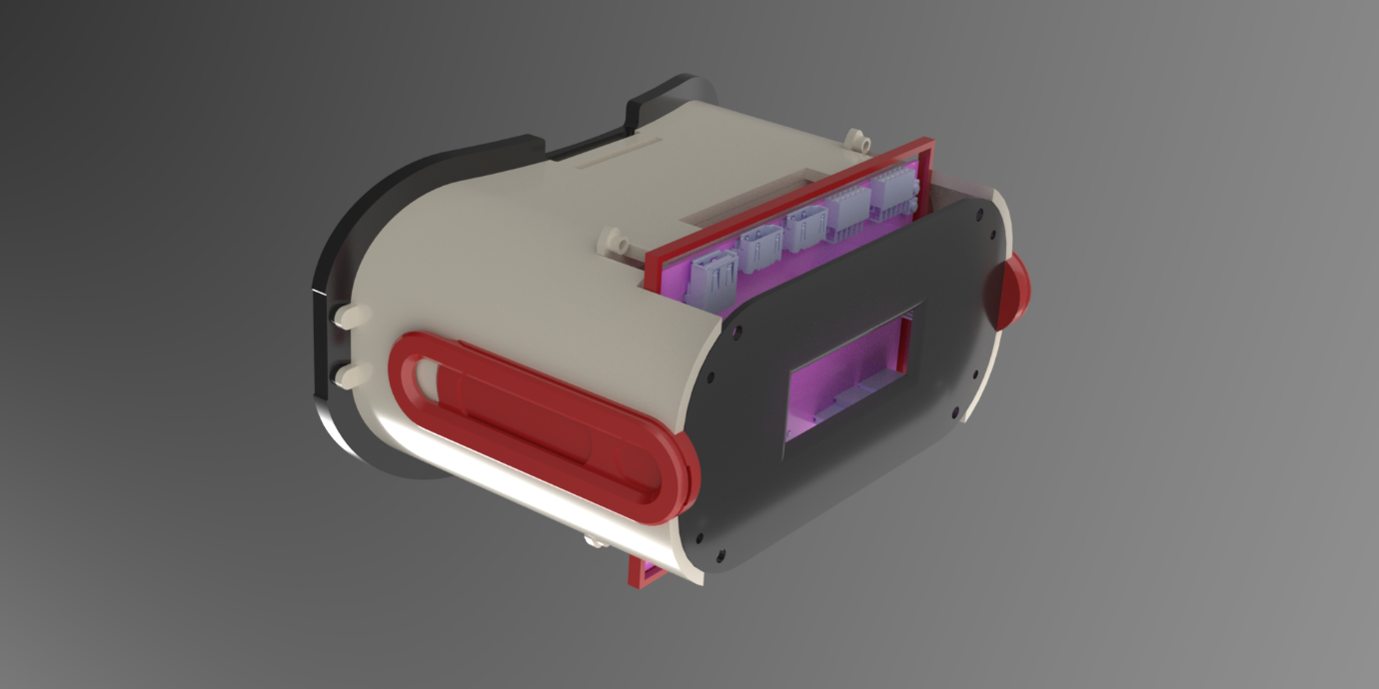
\includegraphics[width=\textwidth,height=0.28\textheight,keepaspectratio]{imgs/Headset_Images/final_rendered.png}
    \caption{Final SolidWorks Visualize render of the complete headset assembly prior to 3D printing.}
\end{subfigure}

\vfill

\begin{subfigure}[b]{0.48\textwidth}
    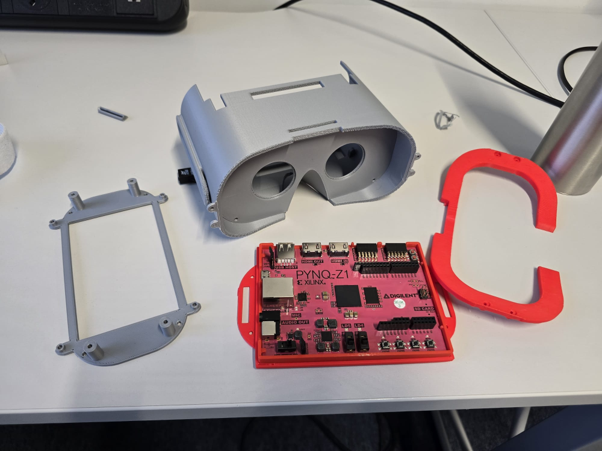
\includegraphics[width=\textwidth,height=0.28\textheight,keepaspectratio]{imgs/Headset_Images/physical_construction.png}
    \caption{Physical construction phase. Parts printed and assembled; minor redesigns for HDMI cable clearance performed here.}
\end{subfigure}\hfill
\begin{subfigure}[b]{0.48\textwidth}
    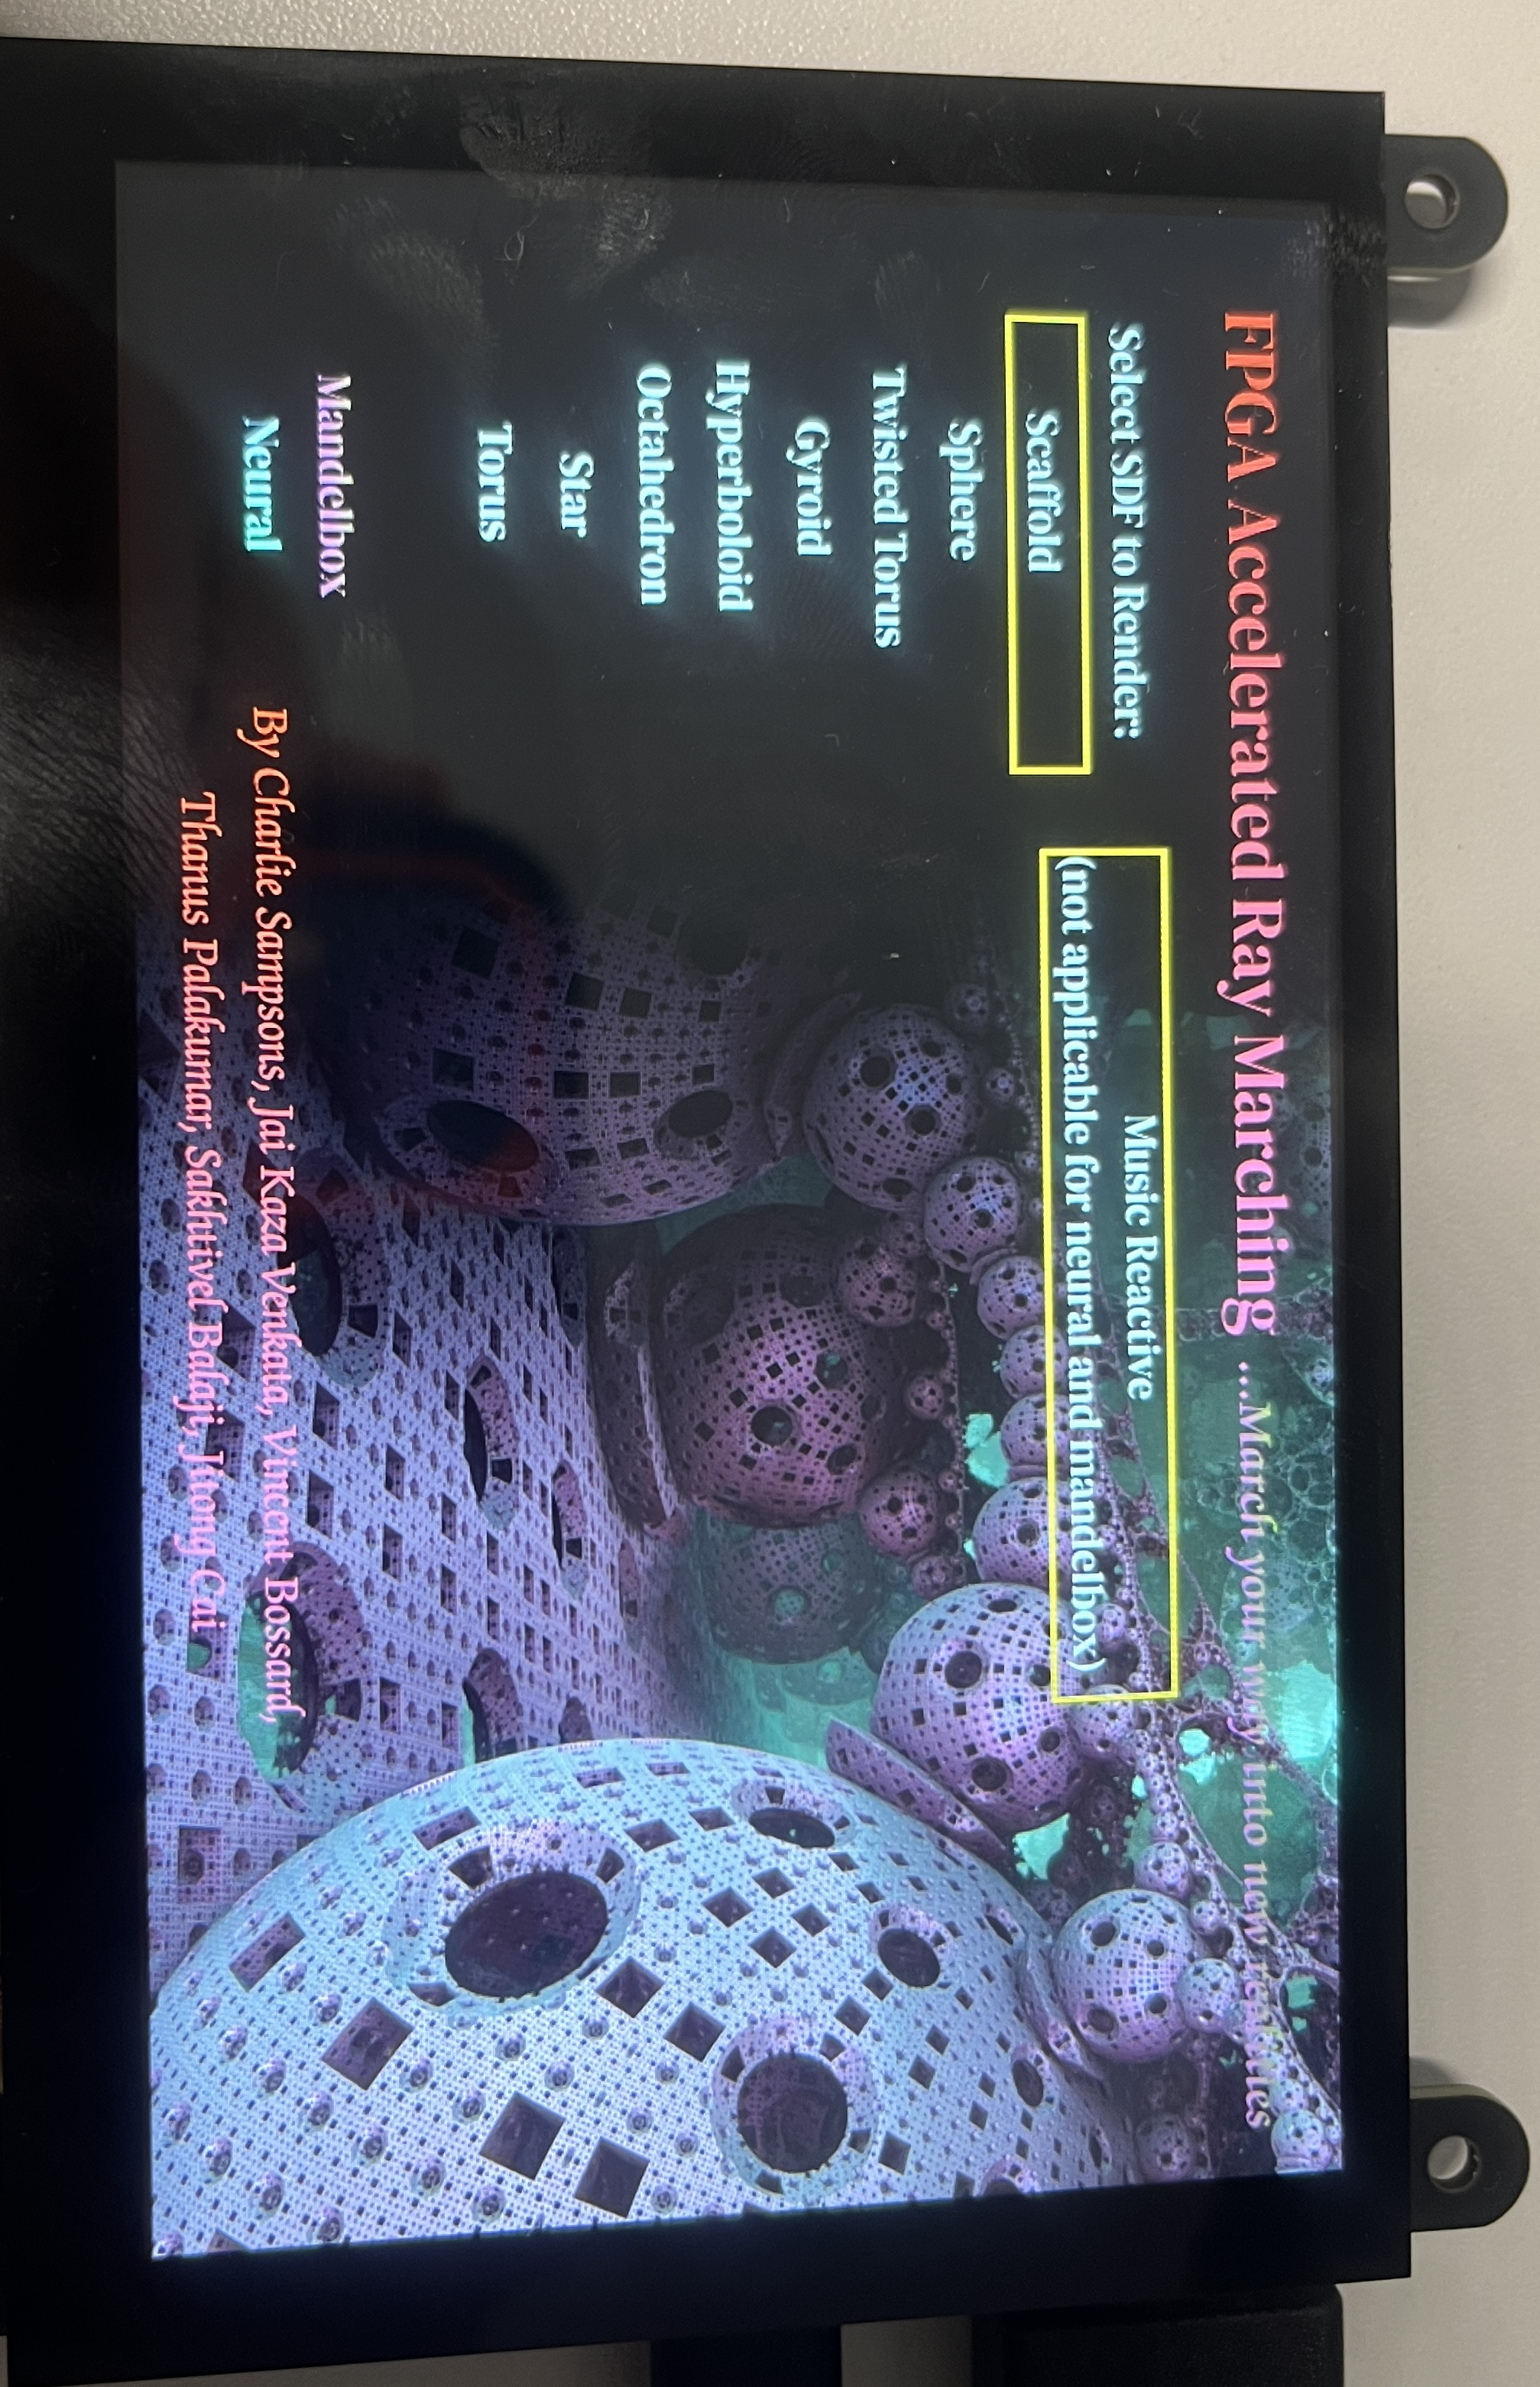
\includegraphics[width=\textwidth,height=0.28\textheight,keepaspectratio]{imgs/ui_no_shift.jpg}
    \caption{Stable scene-selector UI on HDMI output. No frame shift after FCLK0 drop sequence introduced during bitstream swap.}
\end{subfigure}
\caption{VR headset CAD gallery II and system UI --- final design, physical build, and stable display output.}
\end{figure}


% Bibliography Compilation
\cleardoublepage
\nocite{*}
\printbibliography

\end{document}